\documentclass[11pt,a4paper,final,openright]{book}
\usepackage{luatextra}
\usepackage[utf8x]{luainputenc}

\usepackage{amsmath}
\usepackage{amssymb}
\usepackage{amsthm}
\usepackage[toc,page]{appendix}
\usepackage[autostyle=true]{csquotes}
\usepackage{polyglossia} \setmainlanguage{english} % before biblatex
\usepackage[backend=bibtex,natbib=true]{biblatex}
\usepackage{booktabs}
\usepackage[centerlast,small,sc]{caption}
\usepackage{fontspec}
\usepackage{graphicx}
\usepackage[makeindex]{imakeidx}  % dep: before hyperref
\usepackage{hyperref} % dep: after biblatex
\usepackage{import}
\usepackage{microtype}
%\usepackage[oldstyle]{libertine} % (or 'lining')  % alternatives: Garamond, Caladea
\usepackage{subfig}
\usepackage{titling}
\usepackage{pxfonts}
\usepackage{xcolor}
\usepackage{xltxtra}
\usepackage{xunicode}

\parskip2pt

\setromanfont[Ligatures=TeX,Numbers=OldStyle,Variant=01,Fractions=On]{Linux Libertine O}
\setromanfont[Ligatures=TeX,Numbers=OldStyle,Variant=01,Fractions=On]{Linux Libertine O}
\setmonofont{Inconsolata}

\makeindex

\captionsetup[figure]{labelfont=bf}

\definecolor{linkcolor}{cmyk}{0.68,0.00,0.71,0.39}
\definecolor{citecolor}{cmyk}{0.60,0.00,0.75,0.51}
\definecolor{urlcolor}{cmyk}{0.59,0.00,0.76,0.44}

\definecolor{gray}{rgb}{0.7,0.7,0.7}
\newcommand{\dnW}[1][A]{\texttt{#1}}
\newcommand{\dnI}[1]{\texttt{#1}}
\newcommand{\dnCx}{\texttt{\color{red}{x}}}
\newcommand{\dnCu}{\texttt{\color{red}{u}}}
\newcommand{\dnCn}{\texttt{\color{red}{n}}}
\newcommand{\dnCz}{\texttt{\color{black}{0}}}
\newcommand{\dnCo}{\texttt{\color{black}{1}}}
\newcommand{\dnCq}{\texttt{\color{black}{?}}}
\newcommand{\dnCa}{\texttt{\color{black}{A}}}
\newcommand{\dnCb}{\texttt{\color{black}{B}}}
\newcommand{\dnCc}{\texttt{\color{black}{C}}}
\newcommand{\dnCd}{\texttt{\color{black}{D}}}
\newcommand{\dnCh}{\texttt{\color{black}{-}}}

\newcommand\boolf[1]{\texttt{#1}}

\hypersetup{
  pdfpagemode={UseOutlines},
  pdftitle={}, % TODO
  pdfauthor={Lukas Prokop},
  pdfkeywords={master thesis, satisfiability, differential cryptanalysis},
  bookmarksopen=true,
  bookmarksopenlevel=0,
  hypertexnames=false,
  colorlinks=true,
  citecolor=citecolor,
  linkcolor=linkcolor,
  urlcolor=urlcolor,
  pdfstartview={FitV},
  unicode,
  breaklinks=true
}

\addbibresource{thesis.bib}
\setcounter{tocdepth}{3}

\author{Lukas Prokop}
\title{Differential cryptanalysis with SAT solvers}

\theoremstyle{definition}

\newtheorem{theorem}{Theorem}
\newtheorem{defi}{Definition}
\newtheorem{prop}{Proposition}

%\newcommand\theauthor{Lukas Prokop}
\newcommand\authormail{admin@lukas-prokop.at}
\newcommand\institute{Institute of Applied Information Processing and Communications}
\newcommand\university{University of Technology, Graz}
\newcommand\supervisor{Florian Mendel}

\begin{document}

\frontmatter
\begin{titlepage}
  \begin{center}
    {\scshape\LARGE \university\par}\vspace{1.2cm}
    \textsc{\Large Master Thesis}\\[0.5cm]

    \hrulefill \\[0.4cm]
    {\huge \bfseries \makeatletter\@title\makeatother\\}\vspace{0.1cm}
    \hrulefill \\[1.5cm]

    \begin{minipage}[t]{0.4\textwidth}
      \begin{flushleft} \large
        \emph{Author:}\\[3pt]
        \href{mailto:\authormail}{\theauthor, \\ BSc~BSc}
      \end{flushleft}
    \end{minipage}
    \begin{minipage}[t]{0.4\textwidth}
      \begin{flushright} \large
        \emph{Supervisor:} \\[3pt]
        {Dipl.-Ing.~Dr.techn. \\ \supervisor}
      \end{flushright}
    \end{minipage}\\[3cm]

    \large \textit{A thesis submitted in fulfillment of the requirements \\ for the master's degree in Computer Science}\\[0.3cm]
    \textit{at the}\\[0.4cm]
    \begin{minipage}{0.4\textwidth}
      \centering
      \institute
    \end{minipage}
    \vspace{2cm}

    {\large \today}\\[2cm]
    \begin{minipage}{0.4\textwidth}
      \centering
      \def\svgwidth{\textwidth}
      \import*{img/}{iaik.pdf_tex}
    \end{minipage}

    \vfill
  \end{center}
\end{titlepage}

\newcommand{\nextoddpage}{
  \if@openright\cleardoublepage\else\clearpage\fi
  \ifdef{\phantomsection}{\phantomsection}{}
}

\newenvironment{declaration}{
  {\nextoddpage}
  %{\space Affidavit}
  {\thispagestyle{plain}}
  {\null\vfil}
  {\noindent%\huge\bfseries{
    \huge{\textsc{Affidavit}}
  %}
  \par\vspace{10pt}}
}{}

\NewDocumentEnvironment{acknowledgements}{}{%
  {\nextoddpage}
  %\tttypeout{\acknowledgementname}
  \thispagestyle{plain}
  \begin{center}{
      %\huge\textit{
      \Large\textsc{Acknowledgements}
      %}
    \par}\end{center}
}{\vfil\vfil\null}

\NewDocumentEnvironment{abstract}{}{%
  {\nextoddpage}
  \thispagestyle{plain}
  \begin{center}{\huge\textsc{Abstract}\par}\end{center}
}{\vfil\vfil\null}



\begin{abstract}%
  \parskip5pt
  Hash functions are ubiquitous in the modern information age. They provide preimage, second preimage
  and collision resistance ensuring data and origin integrity. They are used as cryptographic primitives
  in protocols and applications.

  In August 2006, Wang et al. showed efficient attacks against several hash function designs including
  MD4, MD5, HAVAL-128 and RIPEMD. With these results differential cryptanalysis has been proven useful
  to break collision resistance in hash functions. Over the years advanced attacks based on those
  differential approaches have been developed.

  In this thesis we encode differential attack settings as SAT problems.
  SAT solvers are utilized to solve the problem revealing actual message collisions for a defined message difference.

  \vspace{3pt}
  \textbf{Keywords:} hash function, differential cryptanalysis, MD4, collision resistance, satisfiability, SAT solver
\end{abstract}

\begin{declaration}
  I declare that I have authored this thesis independently, that I have not used other
  than the declared sources/resources, and that I have explicitly indicated all material
  which has been quoted either literally or by content from the sources used.
  The text document uploaded to TUGRAZonline is identical to the present master‘s
  thesis dissertation.

  %\rule[0.5em]{5em}{0.5pt} \hfill{} \rule[0.5em]{5em}{0.5pt} \\
  %Date \hfill{} Digital signature % TODO
  \vspace{120pt}
  \hfill{}\raggedright{(digital signature)}
\end{declaration}

\begin{acknowledgements}%
  \parskip5pt
  First of all I would like to thank my academic advisor for his continuous support
  during this project. Many hours of debugging were involved in writing this
  master thesis project, but thanks to Florian Mendel, this project came to a release
  with nice results.

  I would also like to thank Maria Eichlseder for her great support. Her unique
  way to ask questions brought me back on track several times.
  Mate Soos supported me during my bachelor thesis with SAT related issues
  and his support continued with this master thesis in private conversations.

  Also thanks to Roderick Bloem and Armin Biere who organized a meeting
  one year before submitting this work defining the main approaches involved
  in this thesis.

  And finally I am grateful for the support by Martina,
  who also supported me during good and bad days with this thesis,
  and my parents which provided a prosperous environment to me
  to be able to be where I am today.

  Thank you!
\end{acknowledgements}

All source code is available at \href{http://lukas-prokop.at/proj/megosat}{lukas-prokop.at/proj/megosat}
and published under terms and conditions of Free/Libre Open Source Software.
This document was printed with \LuaLaTeX and Linux Libertine Font.


\listoffigures
\listoftables
\tableofcontents
\mainmatter

\renewcommand*\chappic{img/intro.pdf}
\renewcommand*\chapquote{}
\renewcommand*\chapquotesrc{}
%
\chapter{Introduction}
\label{ch:intro}
\section{Overview}
\label{sec:intro-overview}
%
Hash functions are used as cryptographic primitives in many applications and protocols.
They take an arbitrary input message and provide a hash value. Input message and hash value
are considered as byte strings in a particular encoding.
The hash value is of fixed length and satisfies several properties which make it useful
in a variety of applications.

In this thesis we will consider the hash algorithms MD4 and SHA-256.
They use basic arithmetic functions like addition and bit-level functions
such as XOR to transform an input to a hash value. We use a bit vector
as input to this implementation and all operations applied to this bit vector
will be represented as clauses of a SAT problem. Additionally we represent
differential characteristics of hash collisions as SAT problem. If and only if
satisfiability is given, the particular differential state is achievable
using two different inputs leading to the same output. As far as SAT solvers
return an actual model satisfying that state, we get an actual hash collision
which can be verified and visualized.
If the internal state of the hash algorithm is too large, the attack can be
computationally simplified by modelling only a subset of steps of the hash algorithm
or changing the modelled differential path.

Based on experience with these kind of problems with previous non-SAT-based tools
we aim to apply best practices to a satisfiability setting.
We will discuss which SAT techniques lead to best performance characteristics
for our MD4 and SHA-256 testcases.

\section{Thesis Outline}
\label{sec:intro-outline}
%
This thesis is organized as follows:

\begin{description}
\item[In Chapter~\ref{ch:intro}] we discuss the basic properties and fundamentals
of the tools in discussion including hash functions and SAT solvers. We develop
a theoretical notion of the basic terms, we will use in the following chapters.

\item[In Chapter~\ref{ch:hash-algos}] we introduce the MD4 and SHA-256 hash functions.
Certain design decisions imply certain properties which can be used in differential
cryptanalysis. We discuss those decisions in this chapter after a formal definition
of the function itself.

\item[In Chapter~\ref{ch:dc}] we discuss approaches of differential cryptanalysis.
We begin with work done by Wang, et al. and followingly introduce differential notation
to simplify representation of differential states. This way we can easily dump
hash collisions.

\item[In Chapter~\ref{ch:sat}] we discuss SAT solving. We give a brief overview
over used SAT solvers and discuss how we can speed up SAT solvers for cryptographic
problems.

\item[In Chapter~\ref{ch:sat-features}] we define SAT features which help us to
classify SAT problems. This is a small subproject we did to look at properties
of resulting DIMACS~CNF files.

\item[In Chapter~\ref{ch:results}] we show data as result of our work.
Runtimes are the main part of this chapter, but also results of the SAT~features
project are presented.

\item[In Chapter~\ref{ch:summary}] we suggest future work based on our results.
\end{description}

\renewcommand*\chappic{img/diff-crypt.pdf}
\renewcommand*\chapquote{Just because it's automatic doesn't mean it works.}
\renewcommand*\chapquotesrc{Daniel J. Bernstein}
%
\chapter{Differential cryptanalysis}
\label{ch:dc}
%
In Chapter~\ref{ch:hash} we defined two hash functions. In this chapter
we consider such functions from a differential perspective. Differential
cryptanalysis will turn out to yield successful collision attacks on hash
functions. We introduce a notation to easily represent differential
characteristics.

\section{Motivation}
\label{sec:dc-motivation}
%
In August 2004, Wang et al. published results at Crypto'04~\cite{wang2004} which revealed
that MD4, MD5, HAVAL-128 and RIPEMD can be broken practically using differential cryptanalysis.
Their work is based on preliminary work by Hans Dobbertin~\cite{Dobbertin1998}.
On an IBM~P690 machine, an MD5 collision can be computed in about one hour using this approach.
Collisions for HAVAL-128, MD4 and RIPEMD were found as well. Patrick Stach's \texttt{md4coll.c}
program~\cite{md4coll} implements Wang's approach and can find MD4 collisions in few seconds
on my Thinkpad~x220 setup specified in Appendix~\ref{app:setup}.

Let $n$ denote the digest size, i.e. the size of the hash value $h(x)$ in bits.
Due to the birthday paradox, a collision attack has a generic complexity of $2^{n/2}$
whereas preimage and second preimage attacks have generic complexities of $2^n$.
In other words it is computationally easier to find any two colliding hash values
than the preimage or second preimage for a given hash value.

Following results by Wang et al., differential cryptanalysis was shown as
powerful tool for cryptanalysis of hash algorithms. This thesis applies those
ideas to satisfiability approaches.

\begin{table}[bt]
  \begin{center}
    \begin{tabular}{cccc}
      \hline \hline
      \multicolumn{4}{c}{Message 1} \\
      \hline
        4d7a9c83 & \textbf{d6cb927a} & \textbf{29d5a578} & 57a7a5ee \\
        de748a3c & dcc366b3 & b683a020 & 3b2a5d9f \\
        c69d71b3 & f9e99198 & d79f805e & a63bb2e8 \\
        \textbf{45dc8e31} & 97e31fe5 & 2794bf08 & b9e8c3e9 \\
      \hline
      \multicolumn{4}{c}{Message 2} \\
      \hline
        4d7a9c83 & \textbf{56cb927a} & \textbf{b9d5a578} & 57a7a5ee \\
        de748a3c & dcc366b3 & b683a020 & 3b2a5d9f \\
        c69d71b3 & f9e99198 & d79f805e & a63bb2e8 \\
        \textbf{45dd8e31} & 97e31fe5 & 2794bf08 & b9e8c3e9 \\
      \hline
      \multicolumn{4}{c}{Hash value of Message 1 and Message 2} \\
      \hline
        5f5c1a0d & 71b36046 & 1b5435da & 9b0d807a \\
      \hline \hline
    \end{tabular}
    \caption[Hexadecimal values of one MD4 collisions given in paper~\cite{wang2004}]{
      One of two MD4 hash collisions provided in~\cite{wang2004}.
      A message represents one block of 512~bits.
      %The hash value consists of 128~bits.
      Values are given in hexadecimal, message words are enumerated from
      left to right, top to bottom. Differences are highlighted in
      bold for illustration purposes. For comparison the first bits
      of Message 1 are \texttt{11000001\dots} and the last bits are
      \texttt{\dots10011101}.
    }
    \label{tab:wang-md4-collision1}
  \end{center}
\end{table}

\newpage
\section{Fundamentals}
\label{sec:dc-fundamentals}
%
\index{Hash collision}
\begin{defi}[Hash collision]
  Given a hash function $h$,
  a hash collision is a pair $(x_1, x_2)$ with $x_1 \neq x_2$ such that
  $h(x_1) = h(x_2)$.
\end{defi}

\index{Pseudo-collision}
Pseudo-collisions are also often considered when attacking hash functions.
A \emph{pseudo-collision} is given if a hash collision can be found for a given
hash function, but the initial vectors (IV) can be chosen for each message.

Hash algorithms consume input values as blocks of bits.
As far as the length of the input must not conform to the block size,
padding is applied. Now consider such a block of input values
and another copy of it. We use those two blocks as inputs for two
hash algorithm instances, but provide slight modifications in few bits.
Differential cryptanalysis is based on the idea to consider those execution states
and trace those differences to learn about the propagation of message differences.
Compare this setup with Figure~\ref{tab:collision-attack}.

\index{Avalanche effect}
At the very beginning only the few defined differences are given. But as the
hash algorithm progresses in computation, differences are propagated to more
and more bits. Most likely the final value will differ in many bits, because
of a desirable hash algorithm property called \emph{avalanche effect}.
A small difference in the input should lead to a significant difference
in the output (i.e. visually recognizable).

Visualizing those differences helps the cryptanalyst to find modifications
yielding a small number of differences in the evaluation state. Empirical
results in differential cryptanalysis indicate that sparse characteristics
are desirable, because it is easier to cancel out few differences in the
output compared to many differences.
The cryptanalyst consecutively modifies the input values to eventually
receive a collision in the output value (i.e. $\Delta C = 0 \iff C = C^*$).

\index{Differential path}
\index{Differential characteristic}
\begin{defi}
  The differential state during a computation is called
  \emph{differential characteristic} (also \emph{differential path}).
\end{defi}

\begin{theorem}
  Assuming the number of differences in a differential characteristic is small,
  this characteristic is expected to result in a hash collision with higher probability.
\end{theorem}

\begin{figure}[bt]
  \begin{center}
    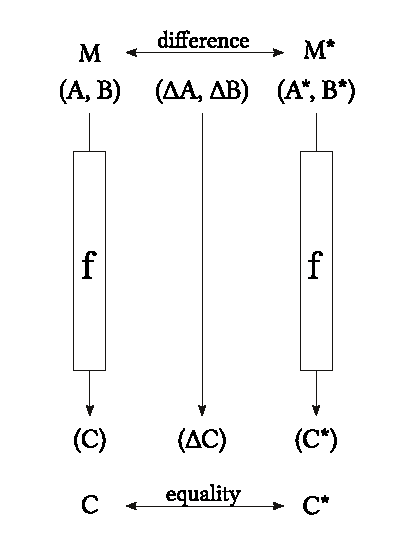
\includegraphics[width=0.55\textwidth]{img/diff_cryptanalysis.pdf}
    \caption[Common attack setting for a collision attack]{
      Common attack setting for a collision attack:
      Hash function $f$ is applied to two inputs $M$ and $M^*$ which differ
      by some predefined bits. $\Delta M$ describes the difference between
      these values. A hash collision is given if and only if output values
      $C$ and $C^*$ show the same value. In differential cryptanalysis we observe
      the differences between two instances applying function $f$
      to inputs $M$ and $M^*$.
    }
    \label{tab:collision-attack}
  \end{center}
\end{figure}

\section{Differential notation}
\label{sec:dc-notation}
%
\index{Bit condition}
\index{Generalized bit condition}
\index{Differential notation}
Differential notation helps us to visualize differential characteristics
by defining so-called \emph{generalized bit conditions}.
It was introduced by Christophe de Canni\`ere and Christian Rechberger
in 2006~\cite[Section 3.2]{char-2006}, inspired by \emph{signed differences} by
Wang~et al. and is shown in Table~\ref{tab:diff-notation}.

\begin{table}[!ht]
  \small
  \begin{center}
    \begin{tabular}{|c|cccc|}
    \hline\hline
      $(x_i, x_i^*)$ & $(0,0)$ & $(1,0)$ & $(0,1)$ & $(1,1)$ \\
    \hline
      \dnI{?}        & \yes    & \yes    & \yes    & \yes    \\
      \dnI{-}        & \yes    & \no     & \no     & \yes    \\
      \dnI{x}        & \no     & \yes    & \yes    & \no     \\
      \dnI{0}        & \yes    & \no     & \no     & \no     \\
      \dnI{u}        & \no     & \yes    & \no     & \no     \\
      \dnI{n}        & \no     & \no     & \yes    & \no     \\
      \dnI{1}        & \no     & \no     & \no     & \yes    \\
      \dnI{\#}       & \no     & \no     & \no     & \no     \\
    \hline \hline
    \end{tabular}
    \begin{tabular}{|c|cccc|}
    \hline\hline
      $(x_i, x_i^*)$ & $(0,0)$ & $(1,0)$ & $(0,1)$ & $(1,1)$ \\
    \hline
      \dnI{3}        & \yes    & \yes    & \no     & \no     \\
      \dnI{5}        & \yes    & \no     & \yes    & \no     \\
      \dnI{7}        & \yes    & \yes    & \yes    & \no     \\
      \dnI{A}        & \no     & \yes    & \no     & \yes    \\
      \dnI{B}        & \yes    & \yes    & \no     & \yes    \\
      \dnI{C}        & \no     & \no     & \yes    & \yes    \\
      \dnI{D}        & \yes    & \no     & \yes    & \yes    \\
      \dnI{E}        & \no     & \yes    & \yes    & \yes    \\
    \hline \hline
    \end{tabular}
    \caption[Differential notation as introduced in~\cite{char-2006}]{
      Differential notation as introduced in~\cite{char-2006}.
      The left-most column specifies a symbol called \enquote{bit condition}
      and right-side columns indicate which bit configurations
      are possible for two given bits $x_i$ and $x_i^*$.
    }
    \label{tab:diff-notation}
  \end{center}
\end{table}

Consider two hash algorithm instances. Let $x_i$ be some bit
from the first instance and let $x_i^*$ be the corresponding bit
from the second instance. Differences are computed using a \boolf{XOR}
and commonly denoted as $\Delta x = x_i \oplus x_i^*$.
Bit conditions allow us to encode possible relations between bits $x_i$ and $x_i^*$.

For example, let us take a look at the original Wang et al. hash collision
in MD4 provided in Table~\ref{tab:wang-md4-collision1}.
We extract all values with differences and represent them using differential notation.
This gives us Table~\ref{tab:differential-wang-values}.

\begin{table}[!ht]
  \begin{center}
    \small
    \begin{tabular}{ccl}
      \hline \hline
      bit & hexadecimal & binary representation / differential notation \\
      \hline \hline
      $x_0$ & \dnI{d6cb927a} & \dnI{11010110110010111001001001111010} \\
      $x_1$ & \dnI{29d5a578} & \dnI{00101001110101011010010101111000} \\
      $x_2$ & \dnI{45dc8e31} & \dnI{01000101110111001000111000110001} \\
      \hline
      $x_0^*$ & \dnI{56cb927a} & \dnI{01010110110010111001001001111010} \\
      $x_1^*$ & \dnI{b9d5a578} & \dnI{10111001110101011010010101111000} \\
      $x_2^*$ & \dnI{45dd8e31} & \dnI{01000101110111011000111000110001} \\
      \hline
      $\Delta x$ & & \dnI{u1010110110010111001001001111010} \\
                 & & \dnI{n01n1001110101011010010101111000} \\
                 & & \dnI{010001011101110n1000111000110001} \\
      \hline \hline
    \end{tabular}
    \caption[Bit differences in the original Wang et al. hash collision]{
      The three words different between Message~1 and Message~2 of the original
      MD4 hash collision by Wang et al. The last three lines show
      how differences can be
      written down using bit conditions. As far as 4 symbols are not from the
      set $\set{0, 1}$ it holds that the messages differ by 4~bits.
    }
    \label{tab:differential-wang-values}
  \end{center}
\end{table}

The following properties hold for bit conditions:
\begin{itemize}[noitemsep,topsep=0pt]
  \item If $x_i = x_i^*$ holds and some value is known, $\set{0,1}$ contains its bit condition.
  \item If $x_i \neq x_i^*$ holds and some value is known, $\set{u,n}$ contains its bit condition.
  \item If $x_i = x_i^*$ holds and the values are unknown, its bit condition is $\dnI{-}$.
  \item If $x_i \neq x_i^*$ holds and the values are unknown, its bit condition is $\dnI{x}$.
\end{itemize}
Applying this notation to hash collisions means that arbitrary bit conditions
(except for \dnI{\#}) can be specified for the input values. In one of the
intermediate iterations, we enforce a difference using one of the bit conditions
$\set{u,n,x}$. This excludes trivial solutions with no differences from the set of
possible solutions. And the final values need to lack differences thus are
represented using a dash \dnI{-}.

\begin{table}[!ht]
  \begin{center}
    \begin{tabular}{cp{5cm}cl}
      $\Delta x$      & conjunctive normal form &
      $\Delta x$      & conjunctive normal form \\
    \hline
      \dnI{\#}        & $(x) \land (\neg x)$ &
      \dnI{1}         & $(x) \land (x^*)$ \\

      \dnI{0}         & $(\neg x) \land (\neg x^*)$ &
      \dnI{-}         & $\neg (x \oplus x^*)$ \\

      \dnI{u}         & $(x) \land (\neg x^*)$ &
      \dnI{A}         & $(x)$ \\

      \dnI{3}         & $(\neg x^*)$ &
      \dnI{B}         & $(x \lor \neg x^*)$ \\

      \dnI{n}         & $(\neg x) \land (x^*)$ &
      \dnI{C}         & $(x^*)$ \\

      \dnI{5}         & $(\neg x)$ &
      \dnI{D}         & $(\neg x \lor x^*)$ \\

      \dnI{x}         & $(x \oplus x^*)$ &
      \dnI{E}         & $(x \lor x^*)$ \\

      \dnI{7}         & $(\neg x \lor \neg x^*)$ &
      \dnI{?}         &  \\
    \end{tabular}
    \caption[Representation of bit conditions as CNF]{%
      All bit conditions represented as CNF using
      two Boolean variables $x$ and $x^*$ to represent
      two bits.
    }
    \label{tab:simple-eval-clauses}
  \end{center}
\end{table}


\section{A simple addition example}
\label{sec:dc-example}
%
Using this notation, we can now reason about the behavior of functions on differential values.
We start with 1-bit addition as basic exercise to the reader. Consider a matrix with
two input rows and one output row. The values of the first two rows are added such that
the bit difference at the third row is created.

\begin{figure}[!ht]
  \begin{center}
    \begin{minipage}{20pt}\begin{tabular}{c} \dnI{-} \\ \dnI{-} \\ \hline \dnI{-} \end{tabular}\end{minipage}
    \hspace{20pt}$\Rightarrow$\hspace{20pt}
    \begin{minipage}{20pt}\begin{tabular}{c} \dnI{0}\dnI{0} \\ \dnI{0}\dnI{0} \\ \hline \dnI{0}\dnI{0} \end{tabular}\end{minipage}
    \begin{minipage}{20pt}\begin{tabular}{c} \dnI{0}\dnI{0} \\ \dnI{0}\dnI{0} \\ \hline \dnI{1}\dnI{1} \end{tabular}\end{minipage}
    \begin{minipage}{20pt}\begin{tabular}{c} \dnI{0}\dnI{0} \\ \dnI{1}\dnI{1} \\ \hline \dnI{0}\dnI{0} \end{tabular}\end{minipage}
    \begin{minipage}{20pt}\begin{tabular}{c} \dnI{0}\dnI{0} \\ \dnI{1}\dnI{1} \\ \hline \dnI{1}\dnI{1} \end{tabular}\end{minipage}
    \begin{minipage}{20pt}\begin{tabular}{c} \dnI{1}\dnI{1} \\ \dnI{0}\dnI{0} \\ \hline \dnI{0}\dnI{0} \end{tabular}\end{minipage}
    \begin{minipage}{20pt}\begin{tabular}{c} \dnI{1}\dnI{1} \\ \dnI{0}\dnI{0} \\ \hline \dnI{1}\dnI{1} \end{tabular}\end{minipage}
    \begin{minipage}{20pt}\begin{tabular}{c} \dnI{1}\dnI{1} \\ \dnI{1}\dnI{1} \\ \hline \dnI{0}\dnI{0} \end{tabular}\end{minipage}
    \begin{minipage}{20pt}\begin{tabular}{c} \dnI{1}\dnI{1} \\ \dnI{1}\dnI{1} \\ \hline \dnI{1}\dnI{1} \end{tabular}\end{minipage}
    \caption[A simple 1-bit addition example]{%
      A simple 1-bit addition example:
      On the left the differential characteristic is given.
      Two dashes, by definition, denote a missing difference in both arguments.
      The result of the addition must never show a difference.
      This yields eight possible bit configurations where two values close to each other denote $(M, M^*)$ of Figure~\ref{tab:collision-attack}.
      Due to the behavior of addition, we know that configurations 2, 3, 5 and 8 (from left to right) are invalid.
    }
    \label{fig:1-bit-example}
  \end{center}
\end{figure}

Figure~\ref{fig:1-bit-example} illustrates this example. Remember that symbols such as
\dnI{-} and \dnI{0} underlie semantics defined in Table~\ref{tab:diff-notation}.
It is also interesting to see how propagation of values can work. In
Figure~\ref{fig:1-bit-deduction} we see how an underspecified value \dnI{?} can be
strengthened once we have checked which values can be taken. Recognize that the
system is constrained by the function in use and the definition of the differential symbols.

\begin{figure}[!ht]
  \begin{center}
    \begin{minipage}{20pt}\begin{tabular}{c} \dnI{-} \\ \dnI{-} \\ \hline \dnI{?} \end{tabular}\end{minipage}
    \hspace{20pt}$\Rightarrow$\hspace{20pt}
    \begin{minipage}{20pt}\begin{tabular}{c} \dnI{0}\dnI{0} \\ \dnI{0}\dnI{0} \\ \hline \dnI{0}\dnI{0} \end{tabular}\end{minipage}
    \begin{minipage}{20pt}\begin{tabular}{c} \dnI{0}\dnI{0} \\ \dnI{1}\dnI{1} \\ \hline \dnI{1}\dnI{1} \end{tabular}\end{minipage}
    \begin{minipage}{20pt}\begin{tabular}{c} \dnI{1}\dnI{1} \\ \dnI{0}\dnI{0} \\ \hline \dnI{1}\dnI{1} \end{tabular}\end{minipage}
    \begin{minipage}{20pt}\begin{tabular}{c} \dnI{1}\dnI{1} \\ \dnI{1}\dnI{1} \\ \hline \dnI{0}\dnI{0} \end{tabular}\end{minipage}
    \caption[Propagation of bit conditions in a differential characteristic]{%
      Like Figure~\ref{fig:1-bit-example}, but any difference value for the result bit is possible.
      As such we consider any possible bit configuration, but eventually recognize that only four bit configurations
      are consistent with the behavior of addition. Because all resulting configurations show no bit difference
      in the output bit, we can strengthen \dnI{?} by replacing it with \dnI{-}. This illustrates how
      knowledge about differential states can be propagated.
    }
    \label{fig:1-bit-deduction}
  \end{center}
\end{figure}

Finally, we can extend our testcases to 4~bits and retrieve testcases such as
Figures~\ref{fig:4-bit-addition} and \ref{fig:sigma}.

\begin{figure}[!ht]
  \begin{center}
    \begin{minipage}{0.23\textwidth}
      \begin{tabular}{rl}
        A: & \dnI{0}\dnI{0}\dnI{1}\dnI{1} \\
        B: & \dnI{0}\dnI{1}\dnI{0}\dnI{1} \\
        S: & \dnI{1}\dnI{0}\dnI{0}\dnI{0}
      \end{tabular}
    \end{minipage}
    \begin{minipage}{0.23\textwidth}
      \begin{tabular}{rl}
        A: & \dnI{-}\dnI{-}\dnI{-}\dnI{x} \\
        B: & \dnI{-}\dnI{-}\dnI{-}\dnI{x} \\
        S: & \dnI{?}\dnI{?}\dnI{?}\dnI{?}
      \end{tabular}
    \end{minipage}
    \begin{minipage}{0.23\textwidth}
      \begin{tabular}{rl}
        A: & \dnI{-}\dnI{-}\dnI{-}\dnI{x} \\
        B: & \dnI{-}\dnI{-}\dnI{-}\dnI{x} \\
        S: & \dnI{?}\dnI{?}\dnI{?}\dnI{-}
      \end{tabular}
    \end{minipage}
    \begin{minipage}{0.23\textwidth}
      \begin{tabular}{rl}
        A: & \dnI{-}\dnI{-}\dnI{-}\dnI{x} \\
        B: & \dnI{-}\dnI{-}\dnI{-}\dnI{x} \\
        S: & \dnI{x}\dnI{?}\dnI{?}\dnI{?}
      \end{tabular}
    \end{minipage}
  \end{center}%

  \begin{center}
    \begin{minipage}{0.23\textwidth}
      \begin{tabular}{rl}
        A: & \dnI{0}\dnI{0}\dnI{1}\dnI{1} \\
        B: & \dnI{0}\dnI{1}\dnI{0}\dnI{1} \\
        S: & \dnI{0}\dnI{0}\dnI{0}\dnI{0}
      \end{tabular}
    \end{minipage}
    \begin{minipage}{0.23\textwidth}
      \begin{tabular}{rl}
        A: & \dnI{-}\dnI{-}\dnI{-}\dnI{x} \\
        B: & \dnI{-}\dnI{-}\dnI{-}\dnI{x} \\
        S: & \dnI{?}\dnI{?}\dnI{?}\dnI{x}
      \end{tabular}
    \end{minipage}
    \begin{minipage}{0.23\textwidth}
      \begin{tabular}{rl}
        A: & \dnI{-}\dnI{-}\dnI{-}\dnI{-} \\
        B: & \dnI{-}\dnI{-}\dnI{-}\dnI{x} \\
        S: & \dnI{x}\dnI{-}\dnI{?}\dnI{?}
      \end{tabular}
    \end{minipage}
  \end{center}%
  \caption[
    Testcases for 4-bit addition
  ]{
    Testcases for 4-bit addition:
    The upper line shows valid differential characteristics for 4-bit addition
    whereas the lower line show invalid ones for 4-bit addition.
    The rows are conventionally named using capital letters.
  }
  \label{fig:4-bit-addition}
\end{figure}

\begin{figure}[!ht]
  \begin{center}
    \begin{minipage}{0.23\textwidth}
      \begin{tabular}{rl}
        A: & \dnI{-}\dnI{-}\dnI{-}\dnI{-} \\
        S: & \dnI{0}\dnI{0}\dnI{0}\dnI{0}
      \end{tabular}
    \end{minipage}
    \begin{minipage}{0.23\textwidth}
      \begin{tabular}{rl}
        A: & \dnI{7}\dnI{C}\dnI{-}\dnI{3} \\
        S: & \dnI{-}\dnI{3}\dnI{u}\dnI{?}
      \end{tabular}
    \end{minipage}
    \begin{minipage}{0.23\textwidth}
      \begin{tabular}{rl}
        A: & \dnI{0}\dnI{u}\dnI{C}\dnI{D} \\
        S: & \dnI{A}\dnI{D}\dnI{C}\dnI{7} \\
      \end{tabular}
    \end{minipage}
  \end{center}

  \begin{center}
    \begin{minipage}{0.23\textwidth}
      \begin{tabular}{rl}
        A: & \dnI{-}\dnI{-}\dnI{-}\dnI{x} \\
        S: & \dnI{0}\dnI{0}\dnI{0}\dnI{0}
      \end{tabular}
    \end{minipage}
    \begin{minipage}{0.23\textwidth}
      \begin{tabular}{rl}
        A: & \dnI{x}\dnI{x}\dnI{x}\dnI{x} \\
        S: & \dnI{0}\dnI{0}\dnI{0}\dnI{0} \\
      \end{tabular}
    \end{minipage}
  \end{center}
  \caption[Differential characteristics for the SHA-2 Sigma function]{
    Differential characteristics for the SHA-2 Sigma function.
    The upper line shows valid states. The lower line shows invalid ones.
  }
  \label{fig:sigma}
\end{figure}

\section{Differential characteristics in action}
\label{sec:dc-actual-chars}
%
In the previous section, we illustrated how propagation with differential values
works and how differential characteristics are written down. It is always
important to keep in mind which function the characteristic illustrates,
because this is not documented with the characteristic.

Now consider MD4 as defined in Section~\ref{sec:dc-md4}. MD4 takes some input
message (in our case limited to size of one block), the state variables
are initialized and iteratively new $A_i$ are computed.

Similarly, SHA-256 takes a message block $M$ and initializes eight
variables with an initial vector (IV). The remaining $W_i$ are computed
and iteratively, values $A_i$ and $E_i$ are computed.

Those values are structured in differential characteristics illustrated
in Figure~\ref{img:char-layouts}. Those layouts are used to specify our
hash collisions we want to evaluate. Table~\ref{tab:wang-collision-propagated}
also gives an application of the layout.

\begin{figure}[!ht]
  \begin{center}
    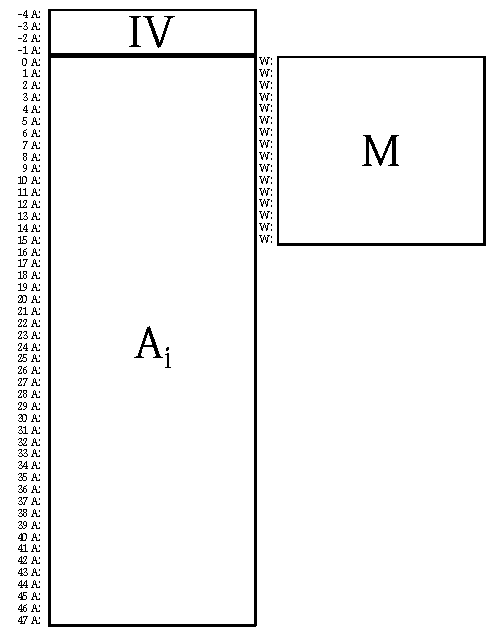
\includegraphics[width=0.4\linewidth]{img/md4_layout.pdf}
    ~~
    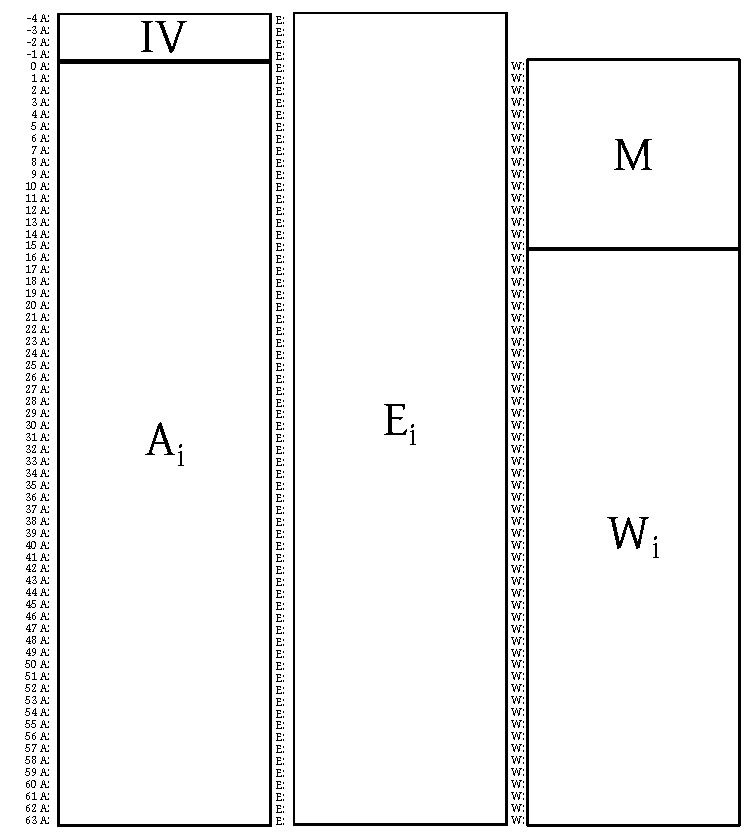
\includegraphics[width=0.5\linewidth]{img/sha256_layout.pdf}
    \caption{Layout of MD4 (left) and SHA-256 (right) differential characteristics}
    \label{img:char-layouts}
  \end{center}
\end{figure}


\texttt{
\begin{table}[p]
\begin{center}
\scalebox{.37}{
\begin{tabular}{|r|c|c|c|c|}
\hline
  $i$  &      &  $\nabla{S_{i,0}}$  &  $\nabla{S_{i,1}}$  &  $\nabla{S_{i,2}}$ \\
\hline
 \dnI{-4} & \dnW: & {{\dnCz}{\dnCo}{\dnCo}{\dnCz}{\dnCz}{\dnCo}{\dnCo}{\dnCo}{\dnCz}{\dnCo}{\dnCz}{\dnCz}{\dnCz}{\dnCo}{\dnCz}{\dnCo}{\dnCz}{\dnCz}{\dnCo}{\dnCz}{\dnCz}{\dnCz}{\dnCo}{\dnCo}{\dnCz}{\dnCz}{\dnCz}{\dnCz}{\dnCz}{\dnCz}{\dnCz}{\dnCo}} & & \\
 \dnI{-3} & \dnW: & {{\dnCz}{\dnCz}{\dnCz}{\dnCo}{\dnCz}{\dnCz}{\dnCz}{\dnCz}{\dnCz}{\dnCz}{\dnCo}{\dnCo}{\dnCz}{\dnCz}{\dnCo}{\dnCz}{\dnCz}{\dnCo}{\dnCz}{\dnCo}{\dnCz}{\dnCo}{\dnCz}{\dnCz}{\dnCz}{\dnCo}{\dnCo}{\dnCo}{\dnCz}{\dnCo}{\dnCo}{\dnCz}} & & \\
 \dnI{-2} & \dnW: & {{\dnCo}{\dnCz}{\dnCz}{\dnCo}{\dnCo}{\dnCz}{\dnCz}{\dnCz}{\dnCo}{\dnCz}{\dnCo}{\dnCo}{\dnCo}{\dnCz}{\dnCo}{\dnCz}{\dnCo}{\dnCo}{\dnCz}{\dnCo}{\dnCo}{\dnCo}{\dnCz}{\dnCz}{\dnCo}{\dnCo}{\dnCo}{\dnCo}{\dnCo}{\dnCo}{\dnCo}{\dnCz}} & & \\
 \dnI{-1} & \dnW: & {{\dnCo}{\dnCo}{\dnCo}{\dnCz}{\dnCo}{\dnCo}{\dnCo}{\dnCo}{\dnCo}{\dnCo}{\dnCz}{\dnCz}{\dnCo}{\dnCo}{\dnCz}{\dnCo}{\dnCo}{\dnCz}{\dnCo}{\dnCz}{\dnCo}{\dnCz}{\dnCo}{\dnCo}{\dnCo}{\dnCz}{\dnCz}{\dnCz}{\dnCo}{\dnCz}{\dnCz}{\dnCo}} & & \\
 \dnI{0} & \dnW: & {{\dnCz}{\dnCo}{\dnCo}{\dnCz}{\dnCo}{\dnCz}{\dnCo}{\dnCo}{\dnCo}{\dnCo}{\dnCz}{\dnCo}{\dnCz}{\dnCo}{\dnCz}{\dnCz}{\dnCo}{\dnCo}{\dnCo}{\dnCz}{\dnCz}{\dnCo}{\dnCz}{\dnCz}{\dnCz}{\dnCz}{\dnCz}{\dnCo}{\dnCz}{\dnCz}{\dnCo}{\dnCz}} & \dnW[W]{}: & {{\dnCz}{\dnCo}{\dnCz}{\dnCz}{\dnCo}{\dnCo}{\dnCz}{\dnCo}{\dnCz}{\dnCo}{\dnCo}{\dnCo}{\dnCo}{\dnCz}{\dnCo}{\dnCz}{\dnCo}{\dnCz}{\dnCz}{\dnCo}{\dnCo}{\dnCo}{\dnCz}{\dnCz}{\dnCo}{\dnCz}{\dnCz}{\dnCz}{\dnCz}{\dnCz}{\dnCo}{\dnCo}} \\
 \dnI{1} & \dnW: & {{\dnCz}{\dnCo}{\dnCo}{\dnCo}{\dnCz}{\dnCo}{\dnCo}{\dnCz}{\dnCz}{\dnCo}{\dnCz}{\dnCz}{\dnCo}{\dnCo}{\dnCo}{\dnCo}{\dnCo}{\dnCo}{\dnCo}{\dnCz}{\dnCo}{\dnCo}{\dnCo}{\dnCz}{\dnCz}{\dnCu}{\dnCo}{\dnCo}{\dnCz}{\dnCz}{\dnCz}{\dnCo}} & \dnW[W]{}: & {{\dnCu}{\dnCo}{\dnCz}{\dnCo}{\dnCz}{\dnCo}{\dnCo}{\dnCz}{\dnCo}{\dnCo}{\dnCz}{\dnCz}{\dnCo}{\dnCz}{\dnCo}{\dnCo}{\dnCo}{\dnCz}{\dnCz}{\dnCo}{\dnCz}{\dnCz}{\dnCo}{\dnCz}{\dnCz}{\dnCo}{\dnCo}{\dnCo}{\dnCo}{\dnCz}{\dnCo}{\dnCz}} \\
 \dnI{2} & \dnW: & {{\dnCo}{\dnCz}{\dnCo}{\dnCz}{\dnCo}{\dnCz}{\dnCo}{\dnCo}{\dnCz}{\dnCo}{\dnCz}{\dnCz}{\dnCz}{\dnCz}{\dnCz}{\dnCz}{\dnCz}{\dnCo}{\dnCo}{\dnCo}{\dnCz}{\dnCu}{\dnCz}{\dnCo}{\dnCn}{\dnCo}{\dnCo}{\dnCo}{\dnCz}{\dnCz}{\dnCo}{\dnCz}} & \dnW[W]{}: & {{\dnCn}{\dnCz}{\dnCo}{\dnCn}{\dnCo}{\dnCz}{\dnCz}{\dnCo}{\dnCo}{\dnCo}{\dnCz}{\dnCo}{\dnCz}{\dnCo}{\dnCz}{\dnCo}{\dnCo}{\dnCz}{\dnCo}{\dnCz}{\dnCz}{\dnCo}{\dnCz}{\dnCo}{\dnCz}{\dnCo}{\dnCo}{\dnCo}{\dnCo}{\dnCz}{\dnCz}{\dnCz}} \\
 \dnI{3} & \dnW: & {{\dnCo}{\dnCz}{\dnCo}{\dnCz}{\dnCo}{\dnCo}{\dnCu}{\dnCo}{\dnCz}{\dnCz}{\dnCo}{\dnCo}{\dnCo}{\dnCo}{\dnCz}{\dnCo}{\dnCz}{\dnCo}{\dnCz}{\dnCo}{\dnCz}{\dnCz}{\dnCo}{\dnCz}{\dnCz}{\dnCo}{\dnCz}{\dnCo}{\dnCz}{\dnCz}{\dnCz}{\dnCo}} & \dnW[W]{}: & {{\dnCz}{\dnCo}{\dnCz}{\dnCo}{\dnCz}{\dnCo}{\dnCo}{\dnCo}{\dnCo}{\dnCz}{\dnCo}{\dnCz}{\dnCz}{\dnCo}{\dnCo}{\dnCo}{\dnCo}{\dnCz}{\dnCo}{\dnCz}{\dnCz}{\dnCo}{\dnCz}{\dnCo}{\dnCo}{\dnCo}{\dnCo}{\dnCz}{\dnCo}{\dnCo}{\dnCo}{\dnCz}} \\
 \dnI{4} & \dnW: & {{\dnCz}{\dnCz}{\dnCo}{\dnCz}{\dnCo}{\dnCo}{\dnCz}{\dnCz}{\dnCz}{\dnCo}{\dnCo}{\dnCz}{\dnCz}{\dnCz}{\dnCo}{\dnCo}{\dnCz}{\dnCo}{\dnCz}{\dnCo}{\dnCz}{\dnCo}{\dnCz}{\dnCo}{\dnCo}{\dnCo}{\dnCo}{\dnCo}{\dnCz}{\dnCz}{\dnCo}{\dnCz}} & \dnW[W]{}: & {{\dnCo}{\dnCo}{\dnCz}{\dnCo}{\dnCo}{\dnCo}{\dnCo}{\dnCz}{\dnCz}{\dnCo}{\dnCo}{\dnCo}{\dnCz}{\dnCo}{\dnCz}{\dnCz}{\dnCo}{\dnCz}{\dnCz}{\dnCz}{\dnCo}{\dnCz}{\dnCo}{\dnCz}{\dnCz}{\dnCz}{\dnCo}{\dnCo}{\dnCo}{\dnCo}{\dnCz}{\dnCz}} \\
 \dnI{5} & \dnW: & {{\dnCz}{\dnCz}{\dnCz}{\dnCo}{\dnCo}{\dnCz}{\dnCo}{\dnCz}{\dnCz}{\dnCo}{\dnCo}{\dnCz}{\dnCz}{\dnCz}{\dnCo}{\dnCz}{\dnCo}{\dnCz}{\dnCu}{\dnCo}{\dnCo}{\dnCz}{\dnCo}{\dnCz}{\dnCz}{\dnCz}{\dnCz}{\dnCz}{\dnCz}{\dnCz}{\dnCz}{\dnCo}} & \dnW[W]{}: & {{\dnCo}{\dnCo}{\dnCz}{\dnCo}{\dnCo}{\dnCo}{\dnCz}{\dnCz}{\dnCo}{\dnCo}{\dnCz}{\dnCz}{\dnCz}{\dnCz}{\dnCo}{\dnCo}{\dnCz}{\dnCo}{\dnCo}{\dnCz}{\dnCz}{\dnCo}{\dnCo}{\dnCz}{\dnCo}{\dnCz}{\dnCo}{\dnCo}{\dnCz}{\dnCz}{\dnCo}{\dnCo}} \\
 \dnI{6} & \dnW: & {{\dnCz}{\dnCz}{\dnCz}{\dnCo}{\dnCo}{\dnCz}{\dnCo}{\dnCo}{\dnCz}{\dnCz}{\dnCu}{\dnCn}{\dnCu}{\dnCu}{\dnCo}{\dnCo}{\dnCz}{\dnCz}{\dnCz}{\dnCo}{\dnCz}{\dnCz}{\dnCz}{\dnCz}{\dnCz}{\dnCo}{\dnCo}{\dnCo}{\dnCo}{\dnCz}{\dnCo}{\dnCz}} & \dnW[W]{}: & {{\dnCq}{\dnCq}{\dnCq}{\dnCq}{\dnCq}{\dnCq}{\dnCq}{\dnCq}{\dnCq}{\dnCq}{\dnCq}{\dnCq}{\dnCq}{\dnCq}{\dnCq}{\dnCq}{\dnCq}{\dnCq}{\dnCq}{\dnCq}{\dnCq}{\dnCq}{\dnCq}{\dnCq}{\dnCq}{\dnCq}{\dnCq}{\dnCq}{\dnCq}{\dnCq}{\dnCq}{\dnCq}} \\
 \dnI{7} & \dnW: & {{\dnCz}{\dnCz}{\dnCo}{\dnCz}{\dnCo}{\dnCz}{\dnCo}{\dnCo}{\dnCo}{\dnCz}{\dnCz}{\dnCz}{\dnCz}{\dnCz}{\dnCz}{\dnCo}{\dnCz}{\dnCu}{\dnCn}{\dnCn}{\dnCz}{\dnCo}{\dnCo}{\dnCz}{\dnCz}{\dnCo}{\dnCz}{\dnCo}{\dnCz}{\dnCz}{\dnCz}{\dnCz}} & \dnW[W]{}: & {{\dnCz}{\dnCz}{\dnCo}{\dnCo}{\dnCo}{\dnCz}{\dnCo}{\dnCo}{\dnCz}{\dnCz}{\dnCo}{\dnCz}{\dnCo}{\dnCz}{\dnCo}{\dnCz}{\dnCz}{\dnCo}{\dnCz}{\dnCo}{\dnCo}{\dnCo}{\dnCz}{\dnCo}{\dnCo}{\dnCz}{\dnCz}{\dnCo}{\dnCo}{\dnCo}{\dnCo}{\dnCo}} \\
 \dnI{8} & \dnW: & {{\dnCq}{\dnCq}{\dnCq}{\dnCq}{\dnCq}{\dnCq}{\dnCq}{\dnCq}{\dnCq}{\dnCq}{\dnCq}{\dnCq}{\dnCq}{\dnCq}{\dnCq}{\dnCq}{\dnCq}{\dnCq}{\dnCq}{\dnCq}{\dnCq}{\dnCq}{\dnCq}{\dnCq}{\dnCq}{\dnCq}{\dnCq}{\dnCq}{\dnCq}{\dnCq}{\dnCq}{\dnCq}} & \dnW[W]{}: & {{\dnCo}{\dnCo}{\dnCz}{\dnCz}{\dnCz}{\dnCo}{\dnCo}{\dnCz}{\dnCo}{\dnCz}{\dnCz}{\dnCo}{\dnCo}{\dnCo}{\dnCz}{\dnCo}{\dnCz}{\dnCo}{\dnCo}{\dnCo}{\dnCz}{\dnCz}{\dnCz}{\dnCo}{\dnCo}{\dnCz}{\dnCo}{\dnCo}{\dnCz}{\dnCz}{\dnCo}{\dnCo}} \\
 \dnI{9} & \dnW: & {{\dnCq}{\dnCq}{\dnCq}{\dnCq}{\dnCq}{\dnCq}{\dnCq}{\dnCq}{\dnCq}{\dnCq}{\dnCq}{\dnCq}{\dnCq}{\dnCq}{\dnCq}{\dnCq}{\dnCq}{\dnCq}{\dnCq}{\dnCq}{\dnCq}{\dnCq}{\dnCq}{\dnCq}{\dnCq}{\dnCq}{\dnCq}{\dnCq}{\dnCq}{\dnCq}{\dnCq}{\dnCq}} & \dnW[W]{}: & {{\dnCo}{\dnCo}{\dnCo}{\dnCo}{\dnCo}{\dnCz}{\dnCz}{\dnCo}{\dnCo}{\dnCo}{\dnCo}{\dnCz}{\dnCo}{\dnCz}{\dnCz}{\dnCo}{\dnCo}{\dnCz}{\dnCz}{\dnCo}{\dnCz}{\dnCz}{\dnCz}{\dnCo}{\dnCo}{\dnCz}{\dnCz}{\dnCo}{\dnCo}{\dnCz}{\dnCz}{\dnCz}} \\
 \dnI{10} & \dnW: & {{\dnCo}{\dnCz}{\dnCn}{\dnCz}{\dnCz}{\dnCo}{\dnCz}{\dnCz}{\dnCo}{\dnCz}{\dnCz}{\dnCz}{\dnCz}{\dnCo}{\dnCz}{\dnCo}{\dnCq}{\dnCq}{\dnCq}{\dnCq}{\dnCq}{\dnCq}{\dnCq}{\dnCq}{\dnCq}{\dnCq}{\dnCq}{\dnCq}{\dnCq}{\dnCo}{\dnCo}{\dnCz}} & \dnW[W]{}: & {{\dnCo}{\dnCo}{\dnCz}{\dnCo}{\dnCz}{\dnCo}{\dnCo}{\dnCo}{\dnCo}{\dnCz}{\dnCz}{\dnCo}{\dnCo}{\dnCo}{\dnCo}{\dnCo}{\dnCo}{\dnCz}{\dnCz}{\dnCz}{\dnCz}{\dnCz}{\dnCz}{\dnCz}{\dnCz}{\dnCo}{\dnCz}{\dnCo}{\dnCo}{\dnCo}{\dnCo}{\dnCz}} \\
 \dnI{11} & \dnW: & {{\dnCu}{\dnCo}{\dnCz}{\dnCz}{\dnCz}{\dnCo}{\dnCo}{\dnCz}{\dnCo}{\dnCz}{\dnCo}{\dnCo}{\dnCz}{\dnCo}{\dnCo}{\dnCz}{\dnCq}{\dnCq}{\dnCq}{\dnCq}{\dnCq}{\dnCq}{\dnCq}{\dnCq}{\dnCq}{\dnCq}{\dnCq}{\dnCq}{\dnCq}{\dnCo}{\dnCo}{\dnCo}} & \dnW[W]{}: & {{\dnCo}{\dnCz}{\dnCo}{\dnCz}{\dnCz}{\dnCo}{\dnCo}{\dnCz}{\dnCz}{\dnCz}{\dnCo}{\dnCo}{\dnCo}{\dnCz}{\dnCo}{\dnCo}{\dnCo}{\dnCz}{\dnCo}{\dnCo}{\dnCz}{\dnCz}{\dnCo}{\dnCz}{\dnCo}{\dnCo}{\dnCo}{\dnCz}{\dnCo}{\dnCz}{\dnCz}{\dnCz}} \\
 \dnI{12} & \dnW: & {{\dnCz}{\dnCz}{\dnCo}{\dnCz}{\dnCo}{\dnCo}{\dnCu}{\dnCz}{\dnCz}{\dnCu}{\dnCo}{\dnCz}{\dnCo}{\dnCz}{\dnCo}{\dnCo}{\dnCq}{\dnCq}{\dnCq}{\dnCq}{\dnCq}{\dnCq}{\dnCq}{\dnCq}{\dnCq}{\dnCq}{\dnCq}{\dnCq}{\dnCq}{\dnCz}{\dnCo}{\dnCo}} & \dnW[W]{}: & {{\dnCz}{\dnCo}{\dnCz}{\dnCz}{\dnCz}{\dnCo}{\dnCz}{\dnCo}{\dnCo}{\dnCo}{\dnCz}{\dnCo}{\dnCo}{\dnCo}{\dnCz}{\dnCn}{\dnCo}{\dnCz}{\dnCz}{\dnCz}{\dnCo}{\dnCo}{\dnCo}{\dnCz}{\dnCz}{\dnCz}{\dnCo}{\dnCo}{\dnCz}{\dnCz}{\dnCz}{\dnCo}} \\
 \dnI{13} & \dnW: & {{\dnCo}{\dnCz}{\dnCu}{\dnCn}{\dnCo}{\dnCn}{\dnCz}{\dnCo}{\dnCz}{\dnCz}{\dnCo}{\dnCo}{\dnCz}{\dnCz}{\dnCz}{\dnCo}{\dnCq}{\dnCq}{\dnCq}{\dnCq}{\dnCq}{\dnCq}{\dnCq}{\dnCq}{\dnCq}{\dnCq}{\dnCq}{\dnCq}{\dnCq}{\dnCo}{\dnCz}{\dnCo}} & \dnW[W]{}: & {{\dnCo}{\dnCz}{\dnCz}{\dnCo}{\dnCz}{\dnCo}{\dnCo}{\dnCo}{\dnCo}{\dnCo}{\dnCo}{\dnCz}{\dnCz}{\dnCz}{\dnCo}{\dnCo}{\dnCz}{\dnCz}{\dnCz}{\dnCo}{\dnCo}{\dnCo}{\dnCo}{\dnCo}{\dnCo}{\dnCo}{\dnCo}{\dnCz}{\dnCz}{\dnCo}{\dnCz}{\dnCo}} \\
 \dnI{14} & \dnW: & {{\dnCz}{\dnCz}{\dnCz}{\dnCz}{\dnCo}{\dnCz}{\dnCo}{\dnCz}{\dnCz}{\dnCo}{\dnCz}{\dnCo}{\dnCz}{\dnCz}{\dnCz}{\dnCo}{\dnCh}{\dnCh}{\dnCh}{\dnCh}{\dnCh}{\dnCh}{\dnCh}{\dnCh}{\dnCh}{\dnCh}{\dnCh}{\dnCh}{\dnCh}{\dnCo}{\dnCo}{\dnCz}} & \dnW[W]{}: & {{\dnCz}{\dnCz}{\dnCo}{\dnCz}{\dnCz}{\dnCo}{\dnCo}{\dnCo}{\dnCo}{\dnCz}{\dnCz}{\dnCo}{\dnCz}{\dnCo}{\dnCz}{\dnCz}{\dnCo}{\dnCz}{\dnCo}{\dnCo}{\dnCo}{\dnCo}{\dnCo}{\dnCo}{\dnCz}{\dnCz}{\dnCz}{\dnCz}{\dnCo}{\dnCz}{\dnCz}{\dnCz}} \\
 \dnI{15} & \dnW: & {{\dnCz}{\dnCz}{\dnCz}{\dnCo}{\dnCo}{\dnCo}{\dnCo}{\dnCz}{\dnCo}{\dnCz}{\dnCo}{\dnCz}{\dnCo}{\dnCu}{\dnCz}{\dnCo}{\dnCh}{\dnCh}{\dnCh}{\dnCh}{\dnCh}{\dnCh}{\dnCh}{\dnCh}{\dnCh}{\dnCh}{\dnCh}{\dnCh}{\dnCh}{\dnCo}{\dnCz}{\dnCz}} & \dnW[W]{}: & {{\dnCo}{\dnCz}{\dnCo}{\dnCo}{\dnCo}{\dnCz}{\dnCz}{\dnCo}{\dnCo}{\dnCo}{\dnCo}{\dnCz}{\dnCo}{\dnCz}{\dnCz}{\dnCz}{\dnCo}{\dnCo}{\dnCz}{\dnCz}{\dnCz}{\dnCz}{\dnCo}{\dnCo}{\dnCo}{\dnCo}{\dnCo}{\dnCz}{\dnCo}{\dnCz}{\dnCz}{\dnCo}} \\
 \dnI{16} & \dnW: & {{\dnCn}{\dnCz}{\dnCz}{\dnCn}{\dnCz}{\dnCu}{\dnCn}{\dnCz}{\dnCo}{\dnCo}{\dnCz}{\dnCo}{\dnCz}{\dnCz}{\dnCo}{\dnCz}{\dnCh}{\dnCh}{\dnCh}{\dnCh}{\dnCh}{\dnCh}{\dnCh}{\dnCh}{\dnCh}{\dnCh}{\dnCh}{\dnCh}{\dnCh}{\dnCo}{\dnCo}{\dnCo}} & & \\
 \dnI{17} & \dnW: & {{\dnCz}{\dnCz}{\dnCz}{\dnCo}{\dnCo}{\dnCo}{\dnCo}{\dnCo}{\dnCz}{\dnCz}{\dnCo}{\dnCo}{\dnCo}{\dnCz}{\dnCo}{\dnCz}{\dnCh}{\dnCh}{\dnCh}{\dnCh}{\dnCh}{\dnCh}{\dnCh}{\dnCh}{\dnCh}{\dnCh}{\dnCh}{\dnCh}{\dnCh}{\dnCo}{\dnCo}{\dnCz}} & & \\
 \dnI{18} & \dnW: & {{\dnCz}{\dnCo}{\dnCz}{\dnCo}{\dnCz}{\dnCo}{\dnCo}{\dnCo}{\dnCz}{\dnCz}{\dnCz}{\dnCz}{\dnCo}{\dnCo}{\dnCz}{\dnCo}{\dnCh}{\dnCh}{\dnCh}{\dnCh}{\dnCh}{\dnCh}{\dnCh}{\dnCh}{\dnCh}{\dnCh}{\dnCh}{\dnCh}{\dnCh}{\dnCo}{\dnCz}{\dnCz}} & & \\
 \dnI{19} & \dnW: & {{\dnCu}{\dnCo}{\dnCn}{\dnCo}{\dnCz}{\dnCz}{\dnCz}{\dnCz}{\dnCz}{\dnCz}{\dnCz}{\dnCo}{\dnCz}{\dnCo}{\dnCo}{\dnCo}{\dnCh}{\dnCh}{\dnCh}{\dnCh}{\dnCh}{\dnCh}{\dnCh}{\dnCh}{\dnCh}{\dnCh}{\dnCh}{\dnCh}{\dnCh}{\dnCo}{\dnCz}{\dnCz}} & & \\
 \dnI{20} & \dnW: & {{\dnCn}{\dnCo}{\dnCu}{\dnCn}{\dnCo}{\dnCz}{\dnCz}{\dnCo}{\dnCo}{\dnCo}{\dnCo}{\dnCo}{\dnCo}{\dnCo}{\dnCz}{\dnCo}{\dnCo}{\dnCo}{\dnCz}{\dnCo}{\dnCz}{\dnCz}{\dnCz}{\dnCz}{\dnCz}{\dnCz}{\dnCo}{\dnCo}{\dnCz}{\dnCo}{\dnCz}{\dnCz}} & & \\
 \dnI{21} & \dnW: & {{\dnCo}{\dnCo}{\dnCo}{\dnCo}{\dnCz}{\dnCz}{\dnCo}{\dnCo}{\dnCo}{\dnCz}{\dnCo}{\dnCo}{\dnCz}{\dnCz}{\dnCz}{\dnCz}{\dnCz}{\dnCo}{\dnCz}{\dnCo}{\dnCo}{\dnCo}{\dnCo}{\dnCo}{\dnCo}{\dnCo}{\dnCz}{\dnCo}{\dnCz}{\dnCo}{\dnCz}{\dnCz}} & & \\
 \dnI{22} & \dnW: & {{\dnCz}{\dnCo}{\dnCz}{\dnCo}{\dnCo}{\dnCo}{\dnCz}{\dnCo}{\dnCo}{\dnCo}{\dnCz}{\dnCz}{\dnCo}{\dnCo}{\dnCz}{\dnCo}{\dnCz}{\dnCz}{\dnCo}{\dnCo}{\dnCz}{\dnCz}{\dnCo}{\dnCo}{\dnCz}{\dnCz}{\dnCo}{\dnCo}{\dnCo}{\dnCz}{\dnCo}{\dnCz}} & & \\
 \dnI{23} & \dnW: & {{\dnCz}{\dnCo}{\dnCz}{\dnCo}{\dnCz}{\dnCz}{\dnCz}{\dnCz}{\dnCo}{\dnCo}{\dnCo}{\dnCz}{\dnCo}{\dnCo}{\dnCo}{\dnCz}{\dnCo}{\dnCo}{\dnCz}{\dnCz}{\dnCz}{\dnCo}{\dnCo}{\dnCo}{\dnCo}{\dnCz}{\dnCz}{\dnCz}{\dnCo}{\dnCo}{\dnCo}{\dnCo}} & & \\
 \dnI{24} & \dnW: & {{\dnCz}{\dnCz}{\dnCz}{\dnCz}{\dnCz}{\dnCz}{\dnCo}{\dnCz}{\dnCz}{\dnCz}{\dnCz}{\dnCo}{\dnCz}{\dnCz}{\dnCo}{\dnCz}{\dnCz}{\dnCz}{\dnCo}{\dnCo}{\dnCz}{\dnCo}{\dnCo}{\dnCo}{\dnCz}{\dnCz}{\dnCz}{\dnCo}{\dnCo}{\dnCz}{\dnCo}{\dnCz}} & & \\
 \dnI{25} & \dnW: & {{\dnCo}{\dnCz}{\dnCo}{\dnCo}{\dnCz}{\dnCz}{\dnCz}{\dnCz}{\dnCo}{\dnCz}{\dnCz}{\dnCo}{\dnCz}{\dnCo}{\dnCo}{\dnCz}{\dnCz}{\dnCz}{\dnCz}{\dnCo}{\dnCz}{\dnCo}{\dnCz}{\dnCz}{\dnCo}{\dnCo}{\dnCo}{\dnCz}{\dnCo}{\dnCz}{\dnCo}{\dnCz}} & & \\
 \dnI{26} & \dnW: & {{\dnCz}{\dnCz}{\dnCz}{\dnCz}{\dnCo}{\dnCz}{\dnCo}{\dnCz}{\dnCo}{\dnCz}{\dnCz}{\dnCz}{\dnCo}{\dnCz}{\dnCz}{\dnCo}{\dnCz}{\dnCo}{\dnCo}{\dnCo}{\dnCz}{\dnCo}{\dnCo}{\dnCo}{\dnCz}{\dnCo}{\dnCz}{\dnCz}{\dnCz}{\dnCz}{\dnCz}{\dnCo}} & & \\
 \dnI{27} & \dnW: & {{\dnCz}{\dnCz}{\dnCz}{\dnCz}{\dnCz}{\dnCo}{\dnCo}{\dnCz}{\dnCo}{\dnCo}{\dnCo}{\dnCz}{\dnCo}{\dnCo}{\dnCo}{\dnCo}{\dnCz}{\dnCo}{\dnCz}{\dnCo}{\dnCo}{\dnCz}{\dnCo}{\dnCz}{\dnCo}{\dnCz}{\dnCo}{\dnCo}{\dnCz}{\dnCz}{\dnCo}{\dnCo}} & & \\
 \dnI{28} & \dnW: & {{\dnCo}{\dnCz}{\dnCo}{\dnCo}{\dnCz}{\dnCo}{\dnCo}{\dnCz}{\dnCz}{\dnCo}{\dnCz}{\dnCo}{\dnCo}{\dnCo}{\dnCz}{\dnCo}{\dnCz}{\dnCo}{\dnCo}{\dnCz}{\dnCo}{\dnCo}{\dnCz}{\dnCz}{\dnCz}{\dnCz}{\dnCo}{\dnCz}{\dnCz}{\dnCo}{\dnCz}{\dnCo}} & & \\
 \dnI{29} & \dnW: & {{\dnCo}{\dnCz}{\dnCo}{\dnCz}{\dnCz}{\dnCz}{\dnCo}{\dnCz}{\dnCz}{\dnCz}{\dnCz}{\dnCz}{\dnCo}{\dnCo}{\dnCz}{\dnCo}{\dnCz}{\dnCo}{\dnCz}{\dnCz}{\dnCo}{\dnCz}{\dnCz}{\dnCz}{\dnCz}{\dnCo}{\dnCo}{\dnCz}{\dnCo}{\dnCz}{\dnCz}{\dnCo}} & & \\
 \dnI{30} & \dnW: & {{\dnCz}{\dnCz}{\dnCo}{\dnCz}{\dnCo}{\dnCz}{\dnCz}{\dnCo}{\dnCo}{\dnCo}{\dnCz}{\dnCo}{\dnCz}{\dnCo}{\dnCo}{\dnCo}{\dnCo}{\dnCo}{\dnCz}{\dnCz}{\dnCz}{\dnCo}{\dnCo}{\dnCo}{\dnCz}{\dnCo}{\dnCo}{\dnCz}{\dnCz}{\dnCz}{\dnCo}{\dnCo}} & & \\
 \dnI{31} & \dnW: & {{\dnCo}{\dnCo}{\dnCo}{\dnCo}{\dnCo}{\dnCo}{\dnCz}{\dnCz}{\dnCo}{\dnCz}{\dnCz}{\dnCo}{\dnCz}{\dnCz}{\dnCo}{\dnCz}{\dnCo}{\dnCo}{\dnCz}{\dnCo}{\dnCz}{\dnCo}{\dnCo}{\dnCo}{\dnCo}{\dnCz}{\dnCo}{\dnCo}{\dnCz}{\dnCo}{\dnCo}{\dnCz}} & & \\
 \dnI{32} & \dnW: & {{\dnCz}{\dnCo}{\dnCz}{\dnCz}{\dnCo}{\dnCo}{\dnCo}{\dnCo}{\dnCo}{\dnCo}{\dnCz}{\dnCo}{\dnCz}{\dnCz}{\dnCo}{\dnCz}{\dnCz}{\dnCo}{\dnCo}{\dnCz}{\dnCo}{\dnCz}{\dnCz}{\dnCz}{\dnCz}{\dnCz}{\dnCo}{\dnCz}{\dnCo}{\dnCo}{\dnCo}{\dnCo}} & & \\
 \dnI{33} & \dnW: & {{\dnCz}{\dnCz}{\dnCo}{\dnCo}{\dnCo}{\dnCz}{\dnCz}{\dnCz}{\dnCz}{\dnCz}{\dnCo}{\dnCo}{\dnCo}{\dnCo}{\dnCz}{\dnCo}{\dnCz}{\dnCo}{\dnCo}{\dnCz}{\dnCo}{\dnCo}{\dnCo}{\dnCz}{\dnCo}{\dnCo}{\dnCo}{\dnCz}{\dnCz}{\dnCo}{\dnCz}{\dnCz}} & & \\
 \dnI{34} & \dnW: & {{\dnCz}{\dnCz}{\dnCo}{\dnCz}{\dnCz}{\dnCz}{\dnCz}{\dnCz}{\dnCz}{\dnCo}{\dnCo}{\dnCo}{\dnCz}{\dnCo}{\dnCz}{\dnCo}{\dnCo}{\dnCo}{\dnCo}{\dnCz}{\dnCo}{\dnCz}{\dnCz}{\dnCz}{\dnCz}{\dnCz}{\dnCz}{\dnCo}{\dnCz}{\dnCo}{\dnCz}{\dnCo}} & & \\
 \dnI{35} & \dnW: & {{\dnCn}{\dnCz}{\dnCo}{\dnCz}{\dnCz}{\dnCz}{\dnCz}{\dnCz}{\dnCz}{\dnCz}{\dnCo}{\dnCo}{\dnCz}{\dnCz}{\dnCo}{\dnCo}{\dnCz}{\dnCz}{\dnCz}{\dnCz}{\dnCz}{\dnCo}{\dnCz}{\dnCz}{\dnCz}{\dnCo}{\dnCo}{\dnCo}{\dnCz}{\dnCz}{\dnCo}{\dnCz}} & & \\
 \dnI{36} & \dnW: & {{\dnCn}{\dnCz}{\dnCz}{\dnCz}{\dnCz}{\dnCo}{\dnCo}{\dnCo}{\dnCo}{\dnCo}{\dnCo}{\dnCz}{\dnCo}{\dnCz}{\dnCo}{\dnCo}{\dnCo}{\dnCo}{\dnCz}{\dnCo}{\dnCo}{\dnCo}{\dnCo}{\dnCz}{\dnCz}{\dnCo}{\dnCz}{\dnCo}{\dnCo}{\dnCz}{\dnCz}{\dnCo}} & & \\
 \dnI{37} & \dnW: & {{\dnCo}{\dnCo}{\dnCz}{\dnCz}{\dnCo}{\dnCz}{\dnCz}{\dnCz}{\dnCz}{\dnCz}{\dnCz}{\dnCo}{\dnCo}{\dnCz}{\dnCo}{\dnCz}{\dnCz}{\dnCo}{\dnCz}{\dnCz}{\dnCz}{\dnCz}{\dnCo}{\dnCo}{\dnCz}{\dnCz}{\dnCz}{\dnCz}{\dnCo}{\dnCo}{\dnCz}{\dnCz}} & & \\
 \dnI{38} & \dnW: & {{\dnCo}{\dnCz}{\dnCo}{\dnCo}{\dnCz}{\dnCz}{\dnCz}{\dnCz}{\dnCz}{\dnCo}{\dnCo}{\dnCz}{\dnCz}{\dnCo}{\dnCo}{\dnCo}{\dnCo}{\dnCo}{\dnCo}{\dnCz}{\dnCo}{\dnCz}{\dnCz}{\dnCo}{\dnCo}{\dnCz}{\dnCo}{\dnCz}{\dnCo}{\dnCo}{\dnCz}{\dnCz}} & & \\
 \dnI{39} & \dnW: & {{\dnCz}{\dnCz}{\dnCz}{\dnCo}{\dnCz}{\dnCz}{\dnCo}{\dnCz}{\dnCz}{\dnCz}{\dnCz}{\dnCz}{\dnCo}{\dnCz}{\dnCo}{\dnCz}{\dnCz}{\dnCz}{\dnCz}{\dnCo}{\dnCo}{\dnCz}{\dnCo}{\dnCo}{\dnCz}{\dnCz}{\dnCz}{\dnCo}{\dnCo}{\dnCo}{\dnCz}{\dnCz}} & & \\
 \dnI{40} & \dnW: & {{\dnCo}{\dnCo}{\dnCz}{\dnCz}{\dnCz}{\dnCz}{\dnCz}{\dnCz}{\dnCz}{\dnCo}{\dnCz}{\dnCz}{\dnCo}{\dnCz}{\dnCz}{\dnCz}{\dnCz}{\dnCo}{\dnCo}{\dnCo}{\dnCz}{\dnCz}{\dnCz}{\dnCo}{\dnCo}{\dnCz}{\dnCz}{\dnCz}{\dnCz}{\dnCo}{\dnCz}{\dnCo}} & & \\
 \dnI{41} & \dnW: & {{\dnCz}{\dnCz}{\dnCz}{\dnCz}{\dnCz}{\dnCo}{\dnCo}{\dnCz}{\dnCo}{\dnCz}{\dnCz}{\dnCz}{\dnCz}{\dnCo}{\dnCo}{\dnCz}{\dnCo}{\dnCo}{\dnCo}{\dnCo}{\dnCz}{\dnCo}{\dnCz}{\dnCo}{\dnCz}{\dnCz}{\dnCo}{\dnCz}{\dnCz}{\dnCo}{\dnCo}{\dnCz}} & & \\
 \dnI{42} & \dnW: & {{\dnCz}{\dnCo}{\dnCz}{\dnCz}{\dnCo}{\dnCo}{\dnCo}{\dnCz}{\dnCo}{\dnCo}{\dnCz}{\dnCo}{\dnCo}{\dnCo}{\dnCz}{\dnCo}{\dnCo}{\dnCo}{\dnCo}{\dnCo}{\dnCo}{\dnCo}{\dnCo}{\dnCz}{\dnCo}{\dnCz}{\dnCz}{\dnCz}{\dnCz}{\dnCo}{\dnCo}{\dnCz}} & & \\
 \dnI{43} & \dnW: & {{\dnCz}{\dnCo}{\dnCz}{\dnCo}{\dnCz}{\dnCz}{\dnCz}{\dnCz}{\dnCz}{\dnCo}{\dnCo}{\dnCz}{\dnCz}{\dnCz}{\dnCo}{\dnCo}{\dnCo}{\dnCo}{\dnCz}{\dnCo}{\dnCz}{\dnCz}{\dnCz}{\dnCz}{\dnCz}{\dnCo}{\dnCo}{\dnCz}{\dnCo}{\dnCo}{\dnCz}{\dnCo}} & & \\
 \dnI{44} & \dnW: & {{\dnCo}{\dnCo}{\dnCo}{\dnCo}{\dnCo}{\dnCz}{\dnCz}{\dnCz}{\dnCz}{\dnCz}{\dnCz}{\dnCo}{\dnCz}{\dnCo}{\dnCo}{\dnCz}{\dnCo}{\dnCo}{\dnCo}{\dnCo}{\dnCz}{\dnCo}{\dnCo}{\dnCo}{\dnCz}{\dnCz}{\dnCz}{\dnCz}{\dnCo}{\dnCo}{\dnCz}{\dnCz}} & & \\
 \dnI{45} & \dnW: & {{\dnCo}{\dnCz}{\dnCz}{\dnCz}{\dnCo}{\dnCz}{\dnCo}{\dnCz}{\dnCo}{\dnCo}{\dnCz}{\dnCo}{\dnCo}{\dnCz}{\dnCo}{\dnCo}{\dnCz}{\dnCz}{\dnCo}{\dnCz}{\dnCo}{\dnCo}{\dnCz}{\dnCz}{\dnCz}{\dnCz}{\dnCz}{\dnCz}{\dnCz}{\dnCo}{\dnCz}{\dnCz}} & & \\
 \dnI{46} & \dnW: & {{\dnCo}{\dnCz}{\dnCz}{\dnCz}{\dnCz}{\dnCz}{\dnCo}{\dnCz}{\dnCo}{\dnCz}{\dnCz}{\dnCo}{\dnCo}{\dnCz}{\dnCz}{\dnCo}{\dnCz}{\dnCo}{\dnCz}{\dnCo}{\dnCo}{\dnCz}{\dnCz}{\dnCz}{\dnCo}{\dnCo}{\dnCz}{\dnCo}{\dnCo}{\dnCo}{\dnCz}{\dnCz}} & & \\
 \dnI{47} & \dnW: & {{\dnCo}{\dnCz}{\dnCz}{\dnCz}{\dnCz}{\dnCz}{\dnCz}{\dnCo}{\dnCo}{\dnCo}{\dnCo}{\dnCz}{\dnCz}{\dnCo}{\dnCz}{\dnCo}{\dnCo}{\dnCz}{\dnCo}{\dnCo}{\dnCz}{\dnCo}{\dnCz}{\dnCz}{\dnCo}{\dnCz}{\dnCo}{\dnCo}{\dnCo}{\dnCo}{\dnCz}{\dnCo}} & & \\
\hline
\end{tabular}
\hspace{10pt}$\Rightarrow$\hspace{10pt}
\begin{tabular}{|r|c|c|c|c|}
\hline
  $i$  &      &  $\nabla{S_{i,0}}$  &  $\nabla{S_{i,1}}$  &  $\nabla{S_{i,2}}$ \\
\hline
 \dnI{-4} & \dnW: & {{\dnCz}{\dnCo}{\dnCo}{\dnCz}{\dnCz}{\dnCo}{\dnCo}{\dnCo}{\dnCz}{\dnCo}{\dnCz}{\dnCz}{\dnCz}{\dnCo}{\dnCz}{\dnCo}{\dnCz}{\dnCz}{\dnCo}{\dnCz}{\dnCz}{\dnCz}{\dnCo}{\dnCo}{\dnCz}{\dnCz}{\dnCz}{\dnCz}{\dnCz}{\dnCz}{\dnCz}{\dnCo}} & & \\
 \dnI{-3} & \dnW: & {{\dnCz}{\dnCz}{\dnCz}{\dnCo}{\dnCz}{\dnCz}{\dnCz}{\dnCz}{\dnCz}{\dnCz}{\dnCo}{\dnCo}{\dnCz}{\dnCz}{\dnCo}{\dnCz}{\dnCz}{\dnCo}{\dnCz}{\dnCo}{\dnCz}{\dnCo}{\dnCz}{\dnCz}{\dnCz}{\dnCo}{\dnCo}{\dnCo}{\dnCz}{\dnCo}{\dnCo}{\dnCz}} & & \\
 \dnI{-2} & \dnW: & {{\dnCo}{\dnCz}{\dnCz}{\dnCo}{\dnCo}{\dnCz}{\dnCz}{\dnCz}{\dnCo}{\dnCz}{\dnCo}{\dnCo}{\dnCo}{\dnCz}{\dnCo}{\dnCz}{\dnCo}{\dnCo}{\dnCz}{\dnCo}{\dnCo}{\dnCo}{\dnCz}{\dnCz}{\dnCo}{\dnCo}{\dnCo}{\dnCo}{\dnCo}{\dnCo}{\dnCo}{\dnCz}} & & \\
 \dnI{-1} & \dnW: & {{\dnCo}{\dnCo}{\dnCo}{\dnCz}{\dnCo}{\dnCo}{\dnCo}{\dnCo}{\dnCo}{\dnCo}{\dnCz}{\dnCz}{\dnCo}{\dnCo}{\dnCz}{\dnCo}{\dnCo}{\dnCz}{\dnCo}{\dnCz}{\dnCo}{\dnCz}{\dnCo}{\dnCo}{\dnCo}{\dnCz}{\dnCz}{\dnCz}{\dnCo}{\dnCz}{\dnCz}{\dnCo}} & & \\
 \dnI{0} & \dnW: & {{\dnCz}{\dnCo}{\dnCo}{\dnCz}{\dnCo}{\dnCz}{\dnCo}{\dnCo}{\dnCo}{\dnCo}{\dnCz}{\dnCo}{\dnCz}{\dnCo}{\dnCz}{\dnCz}{\dnCo}{\dnCo}{\dnCo}{\dnCz}{\dnCz}{\dnCo}{\dnCz}{\dnCz}{\dnCz}{\dnCz}{\dnCz}{\dnCo}{\dnCz}{\dnCz}{\dnCo}{\dnCz}} & \dnW[W]{}: & {{\dnCz}{\dnCo}{\dnCz}{\dnCz}{\dnCo}{\dnCo}{\dnCz}{\dnCo}{\dnCz}{\dnCo}{\dnCo}{\dnCo}{\dnCo}{\dnCz}{\dnCo}{\dnCz}{\dnCo}{\dnCz}{\dnCz}{\dnCo}{\dnCo}{\dnCo}{\dnCz}{\dnCz}{\dnCo}{\dnCz}{\dnCz}{\dnCz}{\dnCz}{\dnCz}{\dnCo}{\dnCo}} \\
 \dnI{1} & \dnW: & {{\dnCz}{\dnCo}{\dnCo}{\dnCo}{\dnCz}{\dnCo}{\dnCo}{\dnCz}{\dnCz}{\dnCo}{\dnCz}{\dnCz}{\dnCo}{\dnCo}{\dnCo}{\dnCo}{\dnCo}{\dnCo}{\dnCo}{\dnCz}{\dnCo}{\dnCo}{\dnCo}{\dnCz}{\dnCz}{\dnCu}{\dnCo}{\dnCo}{\dnCz}{\dnCz}{\dnCz}{\dnCo}} & \dnW[W]{}: & {{\dnCu}{\dnCo}{\dnCz}{\dnCo}{\dnCz}{\dnCo}{\dnCo}{\dnCz}{\dnCo}{\dnCo}{\dnCz}{\dnCz}{\dnCo}{\dnCz}{\dnCo}{\dnCo}{\dnCo}{\dnCz}{\dnCz}{\dnCo}{\dnCz}{\dnCz}{\dnCo}{\dnCz}{\dnCz}{\dnCo}{\dnCo}{\dnCo}{\dnCo}{\dnCz}{\dnCo}{\dnCz}} \\
 \dnI{2} & \dnW: & {{\dnCo}{\dnCz}{\dnCo}{\dnCz}{\dnCo}{\dnCz}{\dnCo}{\dnCo}{\dnCz}{\dnCo}{\dnCz}{\dnCz}{\dnCz}{\dnCz}{\dnCz}{\dnCz}{\dnCz}{\dnCo}{\dnCo}{\dnCo}{\dnCz}{\dnCu}{\dnCz}{\dnCo}{\dnCn}{\dnCo}{\dnCo}{\dnCo}{\dnCz}{\dnCz}{\dnCo}{\dnCz}} & \dnW[W]{}: & {{\dnCn}{\dnCz}{\dnCo}{\dnCn}{\dnCo}{\dnCz}{\dnCz}{\dnCo}{\dnCo}{\dnCo}{\dnCz}{\dnCo}{\dnCz}{\dnCo}{\dnCz}{\dnCo}{\dnCo}{\dnCz}{\dnCo}{\dnCz}{\dnCz}{\dnCo}{\dnCz}{\dnCo}{\dnCz}{\dnCo}{\dnCo}{\dnCo}{\dnCo}{\dnCz}{\dnCz}{\dnCz}} \\
 \dnI{3} & \dnW: & {{\dnCo}{\dnCz}{\dnCo}{\dnCz}{\dnCo}{\dnCo}{\dnCu}{\dnCo}{\dnCz}{\dnCz}{\dnCo}{\dnCo}{\dnCo}{\dnCo}{\dnCz}{\dnCo}{\dnCz}{\dnCo}{\dnCz}{\dnCo}{\dnCz}{\dnCz}{\dnCo}{\dnCz}{\dnCz}{\dnCo}{\dnCz}{\dnCo}{\dnCz}{\dnCz}{\dnCz}{\dnCo}} & \dnW[W]{}: & {{\dnCz}{\dnCo}{\dnCz}{\dnCo}{\dnCz}{\dnCo}{\dnCo}{\dnCo}{\dnCo}{\dnCz}{\dnCo}{\dnCz}{\dnCz}{\dnCo}{\dnCo}{\dnCo}{\dnCo}{\dnCz}{\dnCo}{\dnCz}{\dnCz}{\dnCo}{\dnCz}{\dnCo}{\dnCo}{\dnCo}{\dnCo}{\dnCz}{\dnCo}{\dnCo}{\dnCo}{\dnCz}} \\
 \dnI{4} & \dnW: & {{\dnCz}{\dnCz}{\dnCo}{\dnCz}{\dnCo}{\dnCo}{\dnCz}{\dnCz}{\dnCz}{\dnCo}{\dnCo}{\dnCz}{\dnCz}{\dnCz}{\dnCo}{\dnCo}{\dnCz}{\dnCo}{\dnCz}{\dnCo}{\dnCz}{\dnCo}{\dnCz}{\dnCo}{\dnCo}{\dnCo}{\dnCo}{\dnCo}{\dnCz}{\dnCz}{\dnCo}{\dnCz}} & \dnW[W]{}: & {{\dnCo}{\dnCo}{\dnCz}{\dnCo}{\dnCo}{\dnCo}{\dnCo}{\dnCz}{\dnCz}{\dnCo}{\dnCo}{\dnCo}{\dnCz}{\dnCo}{\dnCz}{\dnCz}{\dnCo}{\dnCz}{\dnCz}{\dnCz}{\dnCo}{\dnCz}{\dnCo}{\dnCz}{\dnCz}{\dnCz}{\dnCo}{\dnCo}{\dnCo}{\dnCo}{\dnCz}{\dnCz}} \\
 \dnI{5} & \dnW: & {{\dnCz}{\dnCz}{\dnCz}{\dnCo}{\dnCo}{\dnCz}{\dnCo}{\dnCz}{\dnCz}{\dnCo}{\dnCo}{\dnCz}{\dnCz}{\dnCz}{\dnCo}{\dnCz}{\dnCo}{\dnCz}{\dnCu}{\dnCo}{\dnCo}{\dnCz}{\dnCo}{\dnCz}{\dnCz}{\dnCz}{\dnCz}{\dnCz}{\dnCz}{\dnCz}{\dnCz}{\dnCo}} & \dnW[W]{}: & {{\dnCo}{\dnCo}{\dnCz}{\dnCo}{\dnCo}{\dnCo}{\dnCz}{\dnCz}{\dnCo}{\dnCo}{\dnCz}{\dnCz}{\dnCz}{\dnCz}{\dnCo}{\dnCo}{\dnCz}{\dnCo}{\dnCo}{\dnCz}{\dnCz}{\dnCo}{\dnCo}{\dnCz}{\dnCo}{\dnCz}{\dnCo}{\dnCo}{\dnCz}{\dnCz}{\dnCo}{\dnCo}} \\
 \dnI{6} & \dnW: & {{\dnCz}{\dnCz}{\dnCz}{\dnCo}{\dnCo}{\dnCz}{\dnCo}{\dnCo}{\dnCz}{\dnCz}{\dnCu}{\dnCn}{\dnCu}{\dnCu}{\dnCo}{\dnCo}{\dnCz}{\dnCz}{\dnCz}{\dnCo}{\dnCz}{\dnCz}{\dnCz}{\dnCz}{\dnCz}{\dnCo}{\dnCo}{\dnCo}{\dnCo}{\dnCz}{\dnCo}{\dnCz}} & \dnW[W]{}: & {{\dnCo}{\dnCz}{\dnCo}{\dnCo}{\dnCz}{\dnCo}{\dnCo}{\dnCz}{\dnCo}{\dnCz}{\dnCz}{\dnCz}{\dnCz}{\dnCz}{\dnCo}{\dnCo}{\dnCo}{\dnCz}{\dnCo}{\dnCz}{\dnCz}{\dnCz}{\dnCz}{\dnCz}{\dnCz}{\dnCz}{\dnCo}{\dnCz}{\dnCz}{\dnCz}{\dnCz}{\dnCz}} \\
 \dnI{7} & \dnW: & {{\dnCz}{\dnCz}{\dnCo}{\dnCz}{\dnCo}{\dnCz}{\dnCo}{\dnCo}{\dnCo}{\dnCz}{\dnCz}{\dnCz}{\dnCz}{\dnCz}{\dnCz}{\dnCo}{\dnCz}{\dnCu}{\dnCn}{\dnCn}{\dnCz}{\dnCo}{\dnCo}{\dnCz}{\dnCz}{\dnCo}{\dnCz}{\dnCo}{\dnCz}{\dnCz}{\dnCz}{\dnCz}} & \dnW[W]{}: & {{\dnCz}{\dnCz}{\dnCo}{\dnCo}{\dnCo}{\dnCz}{\dnCo}{\dnCo}{\dnCz}{\dnCz}{\dnCo}{\dnCz}{\dnCo}{\dnCz}{\dnCo}{\dnCz}{\dnCz}{\dnCo}{\dnCz}{\dnCo}{\dnCo}{\dnCo}{\dnCz}{\dnCo}{\dnCo}{\dnCz}{\dnCz}{\dnCo}{\dnCo}{\dnCo}{\dnCo}{\dnCo}} \\
 \dnI{8} & \dnW: & {{\dnCz}{\dnCo}{\dnCo}{\dnCo}{\dnCz}{\dnCz}{\dnCo}{\dnCo}{\dnCz}{\dnCz}{\dnCo}{\dnCz}{\dnCz}{\dnCz}{\dnCo}{\dnCu}{\dnCo}{\dnCo}{\dnCo}{\dnCo}{\dnCo}{\dnCo}{\dnCo}{\dnCo}{\dnCo}{\dnCz}{\dnCo}{\dnCo}{\dnCz}{\dnCz}{\dnCz}{\dnCz}} & \dnW[W]{}: & {{\dnCo}{\dnCo}{\dnCz}{\dnCz}{\dnCz}{\dnCo}{\dnCo}{\dnCz}{\dnCo}{\dnCz}{\dnCz}{\dnCo}{\dnCo}{\dnCo}{\dnCz}{\dnCo}{\dnCz}{\dnCo}{\dnCo}{\dnCo}{\dnCz}{\dnCz}{\dnCz}{\dnCo}{\dnCo}{\dnCz}{\dnCo}{\dnCo}{\dnCz}{\dnCz}{\dnCo}{\dnCo}} \\
 \dnI{9} & \dnW: & {{\dnCo}{\dnCz}{\dnCo}{\dnCz}{\dnCo}{\dnCo}{\dnCn}{\dnCz}{\dnCo}{\dnCu}{\dnCn}{\dnCn}{\dnCu}{\dnCz}{\dnCz}{\dnCz}{\dnCo}{\dnCo}{\dnCo}{\dnCo}{\dnCo}{\dnCz}{\dnCz}{\dnCo}{\dnCo}{\dnCz}{\dnCz}{\dnCo}{\dnCo}{\dnCo}{\dnCo}{\dnCo}} & \dnW[W]{}: & {{\dnCo}{\dnCo}{\dnCo}{\dnCo}{\dnCo}{\dnCz}{\dnCz}{\dnCo}{\dnCo}{\dnCo}{\dnCo}{\dnCz}{\dnCo}{\dnCz}{\dnCz}{\dnCo}{\dnCo}{\dnCz}{\dnCz}{\dnCo}{\dnCz}{\dnCz}{\dnCz}{\dnCo}{\dnCo}{\dnCz}{\dnCz}{\dnCo}{\dnCo}{\dnCz}{\dnCz}{\dnCz}} \\
 \dnI{10} & \dnW: & {{\dnCo}{\dnCz}{\dnCn}{\dnCz}{\dnCz}{\dnCo}{\dnCz}{\dnCz}{\dnCo}{\dnCz}{\dnCz}{\dnCz}{\dnCz}{\dnCo}{\dnCz}{\dnCo}{\dnCz}{\dnCo}{\dnCz}{\dnCz}{\dnCz}{\dnCz}{\dnCz}{\dnCz}{\dnCo}{\dnCz}{\dnCo}{\dnCz}{\dnCo}{\dnCo}{\dnCo}{\dnCz}} & \dnW[W]{}: & {{\dnCo}{\dnCo}{\dnCz}{\dnCo}{\dnCz}{\dnCo}{\dnCo}{\dnCo}{\dnCo}{\dnCz}{\dnCz}{\dnCo}{\dnCo}{\dnCo}{\dnCo}{\dnCo}{\dnCo}{\dnCz}{\dnCz}{\dnCz}{\dnCz}{\dnCz}{\dnCz}{\dnCz}{\dnCz}{\dnCo}{\dnCz}{\dnCo}{\dnCo}{\dnCo}{\dnCo}{\dnCz}} \\
 \dnI{11} & \dnW: & {{\dnCu}{\dnCo}{\dnCz}{\dnCz}{\dnCz}{\dnCo}{\dnCo}{\dnCz}{\dnCo}{\dnCz}{\dnCo}{\dnCo}{\dnCz}{\dnCo}{\dnCo}{\dnCz}{\dnCz}{\dnCo}{\dnCz}{\dnCz}{\dnCo}{\dnCz}{\dnCo}{\dnCz}{\dnCo}{\dnCo}{\dnCo}{\dnCo}{\dnCo}{\dnCo}{\dnCo}{\dnCo}} & \dnW[W]{}: & {{\dnCo}{\dnCz}{\dnCo}{\dnCz}{\dnCz}{\dnCo}{\dnCo}{\dnCz}{\dnCz}{\dnCz}{\dnCo}{\dnCo}{\dnCo}{\dnCz}{\dnCo}{\dnCo}{\dnCo}{\dnCz}{\dnCo}{\dnCo}{\dnCz}{\dnCz}{\dnCo}{\dnCz}{\dnCo}{\dnCo}{\dnCo}{\dnCz}{\dnCo}{\dnCz}{\dnCz}{\dnCz}} \\
 \dnI{12} & \dnW: & {{\dnCz}{\dnCz}{\dnCo}{\dnCz}{\dnCo}{\dnCo}{\dnCu}{\dnCz}{\dnCz}{\dnCu}{\dnCo}{\dnCz}{\dnCo}{\dnCz}{\dnCo}{\dnCo}{\dnCo}{\dnCo}{\dnCo}{\dnCo}{\dnCo}{\dnCo}{\dnCz}{\dnCz}{\dnCz}{\dnCo}{\dnCo}{\dnCo}{\dnCo}{\dnCz}{\dnCo}{\dnCo}} & \dnW[W]{}: & {{\dnCz}{\dnCo}{\dnCz}{\dnCz}{\dnCz}{\dnCo}{\dnCz}{\dnCo}{\dnCo}{\dnCo}{\dnCz}{\dnCo}{\dnCo}{\dnCo}{\dnCz}{\dnCn}{\dnCo}{\dnCz}{\dnCz}{\dnCz}{\dnCo}{\dnCo}{\dnCo}{\dnCz}{\dnCz}{\dnCz}{\dnCo}{\dnCo}{\dnCz}{\dnCz}{\dnCz}{\dnCo}} \\
 \dnI{13} & \dnW: & {{\dnCo}{\dnCz}{\dnCu}{\dnCn}{\dnCo}{\dnCn}{\dnCz}{\dnCo}{\dnCz}{\dnCz}{\dnCo}{\dnCo}{\dnCz}{\dnCz}{\dnCz}{\dnCo}{\dnCz}{\dnCo}{\dnCz}{\dnCz}{\dnCz}{\dnCz}{\dnCz}{\dnCo}{\dnCo}{\dnCo}{\dnCo}{\dnCz}{\dnCz}{\dnCo}{\dnCz}{\dnCo}} & \dnW[W]{}: & {{\dnCo}{\dnCz}{\dnCz}{\dnCo}{\dnCz}{\dnCo}{\dnCo}{\dnCo}{\dnCo}{\dnCo}{\dnCo}{\dnCz}{\dnCz}{\dnCz}{\dnCo}{\dnCo}{\dnCz}{\dnCz}{\dnCz}{\dnCo}{\dnCo}{\dnCo}{\dnCo}{\dnCo}{\dnCo}{\dnCo}{\dnCo}{\dnCz}{\dnCz}{\dnCo}{\dnCz}{\dnCo}} \\
 \dnI{14} & \dnW: & {{\dnCz}{\dnCz}{\dnCz}{\dnCz}{\dnCo}{\dnCz}{\dnCo}{\dnCz}{\dnCz}{\dnCo}{\dnCz}{\dnCo}{\dnCz}{\dnCz}{\dnCz}{\dnCo}{\dnCo}{\dnCz}{\dnCz}{\dnCz}{\dnCo}{\dnCz}{\dnCz}{\dnCz}{\dnCo}{\dnCo}{\dnCz}{\dnCo}{\dnCz}{\dnCo}{\dnCo}{\dnCz}} & \dnW[W]{}: & {{\dnCz}{\dnCz}{\dnCo}{\dnCz}{\dnCz}{\dnCo}{\dnCo}{\dnCo}{\dnCo}{\dnCz}{\dnCz}{\dnCo}{\dnCz}{\dnCo}{\dnCz}{\dnCz}{\dnCo}{\dnCz}{\dnCo}{\dnCo}{\dnCo}{\dnCo}{\dnCo}{\dnCo}{\dnCz}{\dnCz}{\dnCz}{\dnCz}{\dnCo}{\dnCz}{\dnCz}{\dnCz}} \\
 \dnI{15} & \dnW: & {{\dnCz}{\dnCz}{\dnCz}{\dnCo}{\dnCo}{\dnCo}{\dnCo}{\dnCz}{\dnCo}{\dnCz}{\dnCo}{\dnCz}{\dnCo}{\dnCu}{\dnCz}{\dnCo}{\dnCz}{\dnCo}{\dnCo}{\dnCz}{\dnCz}{\dnCo}{\dnCo}{\dnCz}{\dnCo}{\dnCo}{\dnCz}{\dnCo}{\dnCz}{\dnCo}{\dnCz}{\dnCz}} & \dnW[W]{}: & {{\dnCo}{\dnCz}{\dnCo}{\dnCo}{\dnCo}{\dnCz}{\dnCz}{\dnCo}{\dnCo}{\dnCo}{\dnCo}{\dnCz}{\dnCo}{\dnCz}{\dnCz}{\dnCz}{\dnCo}{\dnCo}{\dnCz}{\dnCz}{\dnCz}{\dnCz}{\dnCo}{\dnCo}{\dnCo}{\dnCo}{\dnCo}{\dnCz}{\dnCo}{\dnCz}{\dnCz}{\dnCo}} \\
 \dnI{16} & \dnW: & {{\dnCn}{\dnCz}{\dnCz}{\dnCn}{\dnCz}{\dnCu}{\dnCn}{\dnCz}{\dnCo}{\dnCo}{\dnCz}{\dnCo}{\dnCz}{\dnCz}{\dnCo}{\dnCz}{\dnCo}{\dnCz}{\dnCz}{\dnCo}{\dnCo}{\dnCz}{\dnCo}{\dnCo}{\dnCz}{\dnCo}{\dnCz}{\dnCo}{\dnCo}{\dnCo}{\dnCo}{\dnCo}} & & \\
 \dnI{17} & \dnW: & {{\dnCz}{\dnCz}{\dnCz}{\dnCo}{\dnCo}{\dnCo}{\dnCo}{\dnCo}{\dnCz}{\dnCz}{\dnCo}{\dnCo}{\dnCo}{\dnCz}{\dnCo}{\dnCz}{\dnCz}{\dnCz}{\dnCz}{\dnCo}{\dnCz}{\dnCz}{\dnCo}{\dnCz}{\dnCz}{\dnCz}{\dnCz}{\dnCo}{\dnCo}{\dnCo}{\dnCo}{\dnCz}} & & \\
 \dnI{18} & \dnW: & {{\dnCz}{\dnCo}{\dnCz}{\dnCo}{\dnCz}{\dnCo}{\dnCo}{\dnCo}{\dnCz}{\dnCz}{\dnCz}{\dnCz}{\dnCo}{\dnCo}{\dnCz}{\dnCo}{\dnCz}{\dnCz}{\dnCz}{\dnCz}{\dnCz}{\dnCz}{\dnCz}{\dnCz}{\dnCo}{\dnCz}{\dnCz}{\dnCo}{\dnCz}{\dnCo}{\dnCz}{\dnCz}} & & \\
 \dnI{19} & \dnW: & {{\dnCu}{\dnCo}{\dnCn}{\dnCo}{\dnCz}{\dnCz}{\dnCz}{\dnCz}{\dnCz}{\dnCz}{\dnCz}{\dnCo}{\dnCz}{\dnCo}{\dnCo}{\dnCo}{\dnCo}{\dnCz}{\dnCz}{\dnCo}{\dnCo}{\dnCz}{\dnCo}{\dnCz}{\dnCo}{\dnCo}{\dnCz}{\dnCz}{\dnCz}{\dnCo}{\dnCz}{\dnCz}} & & \\
 \dnI{20} & \dnW: & {{\dnCn}{\dnCo}{\dnCu}{\dnCn}{\dnCo}{\dnCz}{\dnCz}{\dnCo}{\dnCo}{\dnCo}{\dnCo}{\dnCo}{\dnCo}{\dnCo}{\dnCz}{\dnCo}{\dnCo}{\dnCo}{\dnCz}{\dnCo}{\dnCz}{\dnCz}{\dnCz}{\dnCz}{\dnCz}{\dnCz}{\dnCo}{\dnCo}{\dnCz}{\dnCo}{\dnCz}{\dnCz}} & & \\
 \dnI{21} & \dnW: & {{\dnCo}{\dnCo}{\dnCo}{\dnCo}{\dnCz}{\dnCz}{\dnCo}{\dnCo}{\dnCo}{\dnCz}{\dnCo}{\dnCo}{\dnCz}{\dnCz}{\dnCz}{\dnCz}{\dnCz}{\dnCo}{\dnCz}{\dnCo}{\dnCo}{\dnCo}{\dnCo}{\dnCo}{\dnCo}{\dnCo}{\dnCz}{\dnCo}{\dnCz}{\dnCo}{\dnCz}{\dnCz}} & & \\
 \dnI{22} & \dnW: & {{\dnCz}{\dnCo}{\dnCz}{\dnCo}{\dnCo}{\dnCo}{\dnCz}{\dnCo}{\dnCo}{\dnCo}{\dnCz}{\dnCz}{\dnCo}{\dnCo}{\dnCz}{\dnCo}{\dnCz}{\dnCz}{\dnCo}{\dnCo}{\dnCz}{\dnCz}{\dnCo}{\dnCo}{\dnCz}{\dnCz}{\dnCo}{\dnCo}{\dnCo}{\dnCz}{\dnCo}{\dnCz}} & & \\
 \dnI{23} & \dnW: & {{\dnCz}{\dnCo}{\dnCz}{\dnCo}{\dnCz}{\dnCz}{\dnCz}{\dnCz}{\dnCo}{\dnCo}{\dnCo}{\dnCz}{\dnCo}{\dnCo}{\dnCo}{\dnCz}{\dnCo}{\dnCo}{\dnCz}{\dnCz}{\dnCz}{\dnCo}{\dnCo}{\dnCo}{\dnCo}{\dnCz}{\dnCz}{\dnCz}{\dnCo}{\dnCo}{\dnCo}{\dnCo}} & & \\
 \dnI{24} & \dnW: & {{\dnCz}{\dnCz}{\dnCz}{\dnCz}{\dnCz}{\dnCz}{\dnCo}{\dnCz}{\dnCz}{\dnCz}{\dnCz}{\dnCo}{\dnCz}{\dnCz}{\dnCo}{\dnCz}{\dnCz}{\dnCz}{\dnCo}{\dnCo}{\dnCz}{\dnCo}{\dnCo}{\dnCo}{\dnCz}{\dnCz}{\dnCz}{\dnCo}{\dnCo}{\dnCz}{\dnCo}{\dnCz}} & & \\
 \dnI{25} & \dnW: & {{\dnCo}{\dnCz}{\dnCo}{\dnCo}{\dnCz}{\dnCz}{\dnCz}{\dnCz}{\dnCo}{\dnCz}{\dnCz}{\dnCo}{\dnCz}{\dnCo}{\dnCo}{\dnCz}{\dnCz}{\dnCz}{\dnCz}{\dnCo}{\dnCz}{\dnCo}{\dnCz}{\dnCz}{\dnCo}{\dnCo}{\dnCo}{\dnCz}{\dnCo}{\dnCz}{\dnCo}{\dnCz}} & & \\
 \dnI{26} & \dnW: & {{\dnCz}{\dnCz}{\dnCz}{\dnCz}{\dnCo}{\dnCz}{\dnCo}{\dnCz}{\dnCo}{\dnCz}{\dnCz}{\dnCz}{\dnCo}{\dnCz}{\dnCz}{\dnCo}{\dnCz}{\dnCo}{\dnCo}{\dnCo}{\dnCz}{\dnCo}{\dnCo}{\dnCo}{\dnCz}{\dnCo}{\dnCz}{\dnCz}{\dnCz}{\dnCz}{\dnCz}{\dnCo}} & & \\
 \dnI{27} & \dnW: & {{\dnCz}{\dnCz}{\dnCz}{\dnCz}{\dnCz}{\dnCo}{\dnCo}{\dnCz}{\dnCo}{\dnCo}{\dnCo}{\dnCz}{\dnCo}{\dnCo}{\dnCo}{\dnCo}{\dnCz}{\dnCo}{\dnCz}{\dnCo}{\dnCo}{\dnCz}{\dnCo}{\dnCz}{\dnCo}{\dnCz}{\dnCo}{\dnCo}{\dnCz}{\dnCz}{\dnCo}{\dnCo}} & & \\
 \dnI{28} & \dnW: & {{\dnCo}{\dnCz}{\dnCo}{\dnCo}{\dnCz}{\dnCo}{\dnCo}{\dnCz}{\dnCz}{\dnCo}{\dnCz}{\dnCo}{\dnCo}{\dnCo}{\dnCz}{\dnCo}{\dnCz}{\dnCo}{\dnCo}{\dnCz}{\dnCo}{\dnCo}{\dnCz}{\dnCz}{\dnCz}{\dnCz}{\dnCo}{\dnCz}{\dnCz}{\dnCo}{\dnCz}{\dnCo}} & & \\
 \dnI{29} & \dnW: & {{\dnCo}{\dnCz}{\dnCo}{\dnCz}{\dnCz}{\dnCz}{\dnCo}{\dnCz}{\dnCz}{\dnCz}{\dnCz}{\dnCz}{\dnCo}{\dnCo}{\dnCz}{\dnCo}{\dnCz}{\dnCo}{\dnCz}{\dnCz}{\dnCo}{\dnCz}{\dnCz}{\dnCz}{\dnCz}{\dnCo}{\dnCo}{\dnCz}{\dnCo}{\dnCz}{\dnCz}{\dnCo}} & & \\
 \dnI{30} & \dnW: & {{\dnCz}{\dnCz}{\dnCo}{\dnCz}{\dnCo}{\dnCz}{\dnCz}{\dnCo}{\dnCo}{\dnCo}{\dnCz}{\dnCo}{\dnCz}{\dnCo}{\dnCo}{\dnCo}{\dnCo}{\dnCo}{\dnCz}{\dnCz}{\dnCz}{\dnCo}{\dnCo}{\dnCo}{\dnCz}{\dnCo}{\dnCo}{\dnCz}{\dnCz}{\dnCz}{\dnCo}{\dnCo}} & & \\
 \dnI{31} & \dnW: & {{\dnCo}{\dnCo}{\dnCo}{\dnCo}{\dnCo}{\dnCo}{\dnCz}{\dnCz}{\dnCo}{\dnCz}{\dnCz}{\dnCo}{\dnCz}{\dnCz}{\dnCo}{\dnCz}{\dnCo}{\dnCo}{\dnCz}{\dnCo}{\dnCz}{\dnCo}{\dnCo}{\dnCo}{\dnCo}{\dnCz}{\dnCo}{\dnCo}{\dnCz}{\dnCo}{\dnCo}{\dnCz}} & & \\
 \dnI{32} & \dnW: & {{\dnCz}{\dnCo}{\dnCz}{\dnCz}{\dnCo}{\dnCo}{\dnCo}{\dnCo}{\dnCo}{\dnCo}{\dnCz}{\dnCo}{\dnCz}{\dnCz}{\dnCo}{\dnCz}{\dnCz}{\dnCo}{\dnCo}{\dnCz}{\dnCo}{\dnCz}{\dnCz}{\dnCz}{\dnCz}{\dnCz}{\dnCo}{\dnCz}{\dnCo}{\dnCo}{\dnCo}{\dnCo}} & & \\
 \dnI{33} & \dnW: & {{\dnCz}{\dnCz}{\dnCo}{\dnCo}{\dnCo}{\dnCz}{\dnCz}{\dnCz}{\dnCz}{\dnCz}{\dnCo}{\dnCo}{\dnCo}{\dnCo}{\dnCz}{\dnCo}{\dnCz}{\dnCo}{\dnCo}{\dnCz}{\dnCo}{\dnCo}{\dnCo}{\dnCz}{\dnCo}{\dnCo}{\dnCo}{\dnCz}{\dnCz}{\dnCo}{\dnCz}{\dnCz}} & & \\
 \dnI{34} & \dnW: & {{\dnCz}{\dnCz}{\dnCo}{\dnCz}{\dnCz}{\dnCz}{\dnCz}{\dnCz}{\dnCz}{\dnCo}{\dnCo}{\dnCo}{\dnCz}{\dnCo}{\dnCz}{\dnCo}{\dnCo}{\dnCo}{\dnCo}{\dnCz}{\dnCo}{\dnCz}{\dnCz}{\dnCz}{\dnCz}{\dnCz}{\dnCz}{\dnCo}{\dnCz}{\dnCo}{\dnCz}{\dnCo}} & & \\
 \dnI{35} & \dnW: & {{\dnCn}{\dnCz}{\dnCo}{\dnCz}{\dnCz}{\dnCz}{\dnCz}{\dnCz}{\dnCz}{\dnCz}{\dnCo}{\dnCo}{\dnCz}{\dnCz}{\dnCo}{\dnCo}{\dnCz}{\dnCz}{\dnCz}{\dnCz}{\dnCz}{\dnCo}{\dnCz}{\dnCz}{\dnCz}{\dnCo}{\dnCo}{\dnCo}{\dnCz}{\dnCz}{\dnCo}{\dnCz}} & & \\
 \dnI{36} & \dnW: & {{\dnCn}{\dnCz}{\dnCz}{\dnCz}{\dnCz}{\dnCo}{\dnCo}{\dnCo}{\dnCo}{\dnCo}{\dnCo}{\dnCz}{\dnCo}{\dnCz}{\dnCo}{\dnCo}{\dnCo}{\dnCo}{\dnCz}{\dnCo}{\dnCo}{\dnCo}{\dnCo}{\dnCz}{\dnCz}{\dnCo}{\dnCz}{\dnCo}{\dnCo}{\dnCz}{\dnCz}{\dnCo}} & & \\
 \dnI{37} & \dnW: & {{\dnCo}{\dnCo}{\dnCz}{\dnCz}{\dnCo}{\dnCz}{\dnCz}{\dnCz}{\dnCz}{\dnCz}{\dnCz}{\dnCo}{\dnCo}{\dnCz}{\dnCo}{\dnCz}{\dnCz}{\dnCo}{\dnCz}{\dnCz}{\dnCz}{\dnCz}{\dnCo}{\dnCo}{\dnCz}{\dnCz}{\dnCz}{\dnCz}{\dnCo}{\dnCo}{\dnCz}{\dnCz}} & & \\
 \dnI{38} & \dnW: & {{\dnCo}{\dnCz}{\dnCo}{\dnCo}{\dnCz}{\dnCz}{\dnCz}{\dnCz}{\dnCz}{\dnCo}{\dnCo}{\dnCz}{\dnCz}{\dnCo}{\dnCo}{\dnCo}{\dnCo}{\dnCo}{\dnCo}{\dnCz}{\dnCo}{\dnCz}{\dnCz}{\dnCo}{\dnCo}{\dnCz}{\dnCo}{\dnCz}{\dnCo}{\dnCo}{\dnCz}{\dnCz}} & & \\
 \dnI{39} & \dnW: & {{\dnCz}{\dnCz}{\dnCz}{\dnCo}{\dnCz}{\dnCz}{\dnCo}{\dnCz}{\dnCz}{\dnCz}{\dnCz}{\dnCz}{\dnCo}{\dnCz}{\dnCo}{\dnCz}{\dnCz}{\dnCz}{\dnCz}{\dnCo}{\dnCo}{\dnCz}{\dnCo}{\dnCo}{\dnCz}{\dnCz}{\dnCz}{\dnCo}{\dnCo}{\dnCo}{\dnCz}{\dnCz}} & & \\
 \dnI{40} & \dnW: & {{\dnCo}{\dnCo}{\dnCz}{\dnCz}{\dnCz}{\dnCz}{\dnCz}{\dnCz}{\dnCz}{\dnCo}{\dnCz}{\dnCz}{\dnCo}{\dnCz}{\dnCz}{\dnCz}{\dnCz}{\dnCo}{\dnCo}{\dnCo}{\dnCz}{\dnCz}{\dnCz}{\dnCo}{\dnCo}{\dnCz}{\dnCz}{\dnCz}{\dnCz}{\dnCo}{\dnCz}{\dnCo}} & & \\
 \dnI{41} & \dnW: & {{\dnCz}{\dnCz}{\dnCz}{\dnCz}{\dnCz}{\dnCo}{\dnCo}{\dnCz}{\dnCo}{\dnCz}{\dnCz}{\dnCz}{\dnCz}{\dnCo}{\dnCo}{\dnCz}{\dnCo}{\dnCo}{\dnCo}{\dnCo}{\dnCz}{\dnCo}{\dnCz}{\dnCo}{\dnCz}{\dnCz}{\dnCo}{\dnCz}{\dnCz}{\dnCo}{\dnCo}{\dnCz}} & & \\
 \dnI{42} & \dnW: & {{\dnCz}{\dnCo}{\dnCz}{\dnCz}{\dnCo}{\dnCo}{\dnCo}{\dnCz}{\dnCo}{\dnCo}{\dnCz}{\dnCo}{\dnCo}{\dnCo}{\dnCz}{\dnCo}{\dnCo}{\dnCo}{\dnCo}{\dnCo}{\dnCo}{\dnCo}{\dnCo}{\dnCz}{\dnCo}{\dnCz}{\dnCz}{\dnCz}{\dnCz}{\dnCo}{\dnCo}{\dnCz}} & & \\
 \dnI{43} & \dnW: & {{\dnCz}{\dnCo}{\dnCz}{\dnCo}{\dnCz}{\dnCz}{\dnCz}{\dnCz}{\dnCz}{\dnCo}{\dnCo}{\dnCz}{\dnCz}{\dnCz}{\dnCo}{\dnCo}{\dnCo}{\dnCo}{\dnCz}{\dnCo}{\dnCz}{\dnCz}{\dnCz}{\dnCz}{\dnCz}{\dnCo}{\dnCo}{\dnCz}{\dnCo}{\dnCo}{\dnCz}{\dnCo}} & & \\
 \dnI{44} & \dnW: & {{\dnCo}{\dnCo}{\dnCo}{\dnCo}{\dnCo}{\dnCz}{\dnCz}{\dnCz}{\dnCz}{\dnCz}{\dnCz}{\dnCo}{\dnCz}{\dnCo}{\dnCo}{\dnCz}{\dnCo}{\dnCo}{\dnCo}{\dnCo}{\dnCz}{\dnCo}{\dnCo}{\dnCo}{\dnCz}{\dnCz}{\dnCz}{\dnCz}{\dnCo}{\dnCo}{\dnCz}{\dnCz}} & & \\
 \dnI{45} & \dnW: & {{\dnCo}{\dnCz}{\dnCz}{\dnCz}{\dnCo}{\dnCz}{\dnCo}{\dnCz}{\dnCo}{\dnCo}{\dnCz}{\dnCo}{\dnCo}{\dnCz}{\dnCo}{\dnCo}{\dnCz}{\dnCz}{\dnCo}{\dnCz}{\dnCo}{\dnCo}{\dnCz}{\dnCz}{\dnCz}{\dnCz}{\dnCz}{\dnCz}{\dnCz}{\dnCo}{\dnCz}{\dnCz}} & & \\
 \dnI{46} & \dnW: & {{\dnCo}{\dnCz}{\dnCz}{\dnCz}{\dnCz}{\dnCz}{\dnCo}{\dnCz}{\dnCo}{\dnCz}{\dnCz}{\dnCo}{\dnCo}{\dnCz}{\dnCz}{\dnCo}{\dnCz}{\dnCo}{\dnCz}{\dnCo}{\dnCo}{\dnCz}{\dnCz}{\dnCz}{\dnCo}{\dnCo}{\dnCz}{\dnCo}{\dnCo}{\dnCo}{\dnCz}{\dnCz}} & & \\
 \dnI{47} & \dnW: & {{\dnCo}{\dnCz}{\dnCz}{\dnCz}{\dnCz}{\dnCz}{\dnCz}{\dnCo}{\dnCo}{\dnCo}{\dnCo}{\dnCz}{\dnCz}{\dnCo}{\dnCz}{\dnCo}{\dnCo}{\dnCz}{\dnCo}{\dnCo}{\dnCz}{\dnCo}{\dnCz}{\dnCz}{\dnCo}{\dnCz}{\dnCo}{\dnCo}{\dnCo}{\dnCo}{\dnCz}{\dnCo}} & & \\
\hline
\end{tabular}
}
\caption[%
  One of the original MD4 collisions by Wang et al,
  with a few bits underspecified and followingly propagated%
]{%
  One of the original MD4 collisions by Wang et al,
  with a few bits underspecified (left) and propagated values (right).
  The question marks indicate that any bit configuration for the two bits
  are possible. Dashes indicate that the bits have the same configuration
  in both instances, but the value itself is unknown.
  However, it turns out the description with missing values in iteration~6
  (message) and iterations 8--19 is complete enough such that missing values
  can be deduced by other values and the description of the algorithm.
  A collision is given in the last 4 rounds, because no differences
  are left as they cancel out after round~36.
}
\label{tab:wang-collision-propagated}
\end{center}
\end{table}
}

\renewcommand*\chappic{img/satisfiability.pdf}
\renewcommand*\chapquote{What idiot called them logic errors rather than bool shit?}
\renewcommand*\chapquotesrc{Unknown}
\chapter{Satisfiability}
\label{ch:sat}
%
Boolean algebra allows us to describe functions over two-valued variables.
Satisfiability is the question for an assignment such that a function
evaluates to true. Satisfiability problems are solved by SAT~solvers.
We discuss the basic theory behind satisfiability. Because any computation
can be represented as satisfiability problem, we are able to verify
whether an algorithm can reach a certain state. In Chapter~\ref{ch:enc},
we will represent a differential cryptanalysis problem such that it is
solvable iff the corresponding SAT~problem is satisfiable.

\section{Basic notation and definitions}
\label{sec:sat-intro}
%
\index{Boolean function}
\begin{defi}[Boolean function]
  A \emph{Boolean function} is a mapping $h: X \to Y$ with $X = \left\{0,1\right\}^n$
  for $n \in \mathbb N_{\geq 1}$ and $Y = \left\{0,1\right\}$.
\end{defi}

\index{Assignment}
\begin{defi}[Assignment]
  A \emph{$k$-assignment} is an element of $\left\{0,1\right\}^k$.

  \noindent
  Let $f$ be some $k$-ary Boolean function.
  An \emph{assignment for function $f$} is any $k$-assignment.
\end{defi}

\index{Truth table}
\begin{defi}[Truth table]
  Let $f$ be some $k$-ary Boolean function.
  The \emph{truth table of Boolean function $f$} assigns
  truth value $0$ or $1$ to any assignment of $f$.
\end{defi}

Boolean functions are characterized by their corresponding truth table.

\begin{table}[pt]
  \centering
  \subfloat[\boolf{AND}]{%
    \begin{tabular}{cc|c}
      $x_1$ & $x_2$ & $f(x_1, x_2)$ \\
     \hline
      $1$ & $1$ & $1$ \\
      $1$ & $0$ & $0$ \\
      $0$ & $1$ & $0$ \\
      $0$ & $0$ & $0$
    \end{tabular}
  }
  ~
  \subfloat[\boolf{OR}]{%
    \begin{tabular}{cc|c}
      $x_1$ & $x_2$ & $f(x_1, x_2)$ \\
     \hline
      $1$ & $1$ & $1$ \\
      $1$ & $0$ & $1$ \\
      $0$ & $1$ & $1$ \\
      $0$ & $0$ & $0$
    \end{tabular}
  }
  ~
  \raisebox{13.6pt}{%
    \subfloat[\boolf{NOT}]{%
      \begin{tabular}{c|c}
        $x$ & $f(x)$ \\
       \hline
        $1$ & $0$ \\
        $0$ & $1$
      \end{tabular}
    }%
  }%
  \caption{Truth tables for \boolf{AND}, \boolf{OR} and \boolf{NOT}}
  \label{tab:andornot-truthtables}
\end{table}

Table~\ref{tab:andornot-truthtables} shows example truth tables for
the Boolean \boolf{AND}, \boolf{OR} and \boolf{NOT} functions.
A different definition of the three functions is given the following way:

\index{AND (Boolean function)}
\index{OR (Boolean function)}
\index{NOT (Boolean function)}
\begin{defi}
  Let \boolf{AND}, \boolf{OR} and \boolf{NOT} be three Boolean functions.
  \begin{itemize}[noitemsep,topsep=0pt]
    \item
      \boolf{AND} maps $X = \left\{0,1\right\}^2$
      to $1$ if all values of $X$ are $1$.
    \item
      \boolf{OR} maps $X = \left\{0,1\right\}^2$
      to $1$ if any value of $X$ is $1$.
    \item
      \boolf{NOT} maps $X = \left\{0,1\right\}^1$
      to $1$ if the single value of $X$ is $0$.
  \end{itemize}
  All functions return $0$ in the other case.
  Those functions are denoted $a_0 \land a_1$, $a_0 \lor a_1$
  and $\neg a_0$ respectively, for input parameters $a_0$ and $a_1$.
\end{defi}

It is interesting to observe, that any Boolean function can be represented
using only these three operators. This can be proven by complete induction
over the number of arguments $k$ of the function.

Let $k = 1$. Then we consider any possible $2$-assignment for one input
variable $x_1$ and one value of $f(x_1)$. Then four truth tables are possible
listed in Table~\ref{tab:unary-f}. The description shows the corresponding
definition of $f$ using \boolf{AND}, \boolf{OR} and \boolf{NOT} only.

Now let $g$ be some $k$-ary function. Let $(a_0, a_1, \ldots, a_k)$ be the
$k$ input arguments to $g$ and $x_1 \coloneqq g(a_0, a_1, \ldots, a_k)$.
Then we can again look at Table~\ref{tab:unary-f} to discover that 4 cases
are possible: 2 cases where the return value of our new $(k+1)$-ary function
depends on value $x_1$ and 2 cases where the return value is constant.

This completes our proof.

\begin{table}[ht]
  \centering
  \subfloat[$f: x \mapsto 1$]{%
    \begin{tabular}{cc}
      $x_1$ & $f(x_1)$ \\
     \hline
      $1$ & $1$ \\
      $0$ & $1$
    \end{tabular}
  }
  ~
  \subfloat[$f: x \mapsto x$]{%
    \begin{tabular}{cc}
      $x_1$ & $f(x_1)$ \\
     \hline
      $1$ & $1$ \\
      $0$ & $0$
    \end{tabular}
  }
  ~
  \subfloat[$f: x \mapsto \neg x$]{%
    \begin{tabular}{cc}
      $x_1$ & $f(x_1)$ \\
     \hline
      $1$ & $0$ \\
      $0$ & $1$
    \end{tabular}
  }
  ~
  \subfloat[$f: x \mapsto 0$]{%
    \begin{tabular}{cc}
      $x_1$ & $f(x_1)$ \\
     \hline
      $1$ & $0$ \\
      $0$ & $0$
    \end{tabular}
  }%
  \caption{Unary $f$ and its four possible cases}
  \label{tab:unary-f}
\end{table}

Boolean functions have an important property which is described
in the following definition:

\index{Satisfiability}
\index{Assignment}
\index{Model}
\begin{defi}
  A Boolean function $f$ is \emph{satisfiable} iff there exists at least one
  input $x \in X$ such that $f(x) = 1$.
  Every input $x \in X$ satisfying this property is called \emph{model}.
\end{defi}

The corresponding tool to determine satisfiability is defined as follows:

\index{SAT solver}
\begin{defi}
  A \emph{SAT solver} is a tool to determine satisfiability (SAT or UNSAT)
  of a Boolean function. If satisfiability is given, it returns some model.
\end{defi}

\subsection{Computational considerations}
\label{sec:sat-complexity}
%
The generic complexity of SAT determination is given by $2^n$ for $n$ Boolean variables.

Let $n$ be the number of variables of a Boolean function.
No known algorithm exists to determine satisfiability in polynomial runtime.
This means no algorithm solves the SAT problem with runtime behavior
which depends polynomially on the growth of $n$.
%
\index{Unit propagation}
However, SAT solvers can take advantage of the problem's description.
For example, consider function $f$:
\begin{align} f(x_0, x_1, x_2) &= x_0 \land (\neg x_1 \lor x_2) \label{eq:3f} \end{align}
Instead of trying all possible 8~cases for 3~Boolean variables,
we can immediately see that $x_0$ is required to be $1$.
So we don't need to test $x_0 = 0$ and can skip 4~cases.
This particular strategy is called \emph{unit propagation}.

\subsection{SAT competitions}
\label{sec:sat-competitions}
%
SAT research is heavily concerned with finding fast heuristics
determining (un)satisfiability. Biyearly,
SAT competitions~\cite{satcomp} take place to challenge
SAT solvers in a set of benchmarks. The committee evaluates the most successful
SAT solvers defined by solving the most problems within a given time frame.

In 2014, lingeling by Armin Biere has won first prize in
the Application benchmarks track and second prize in the Hard Combinatorial benchmarks
track for SAT and UNSAT instances, respectively. Its parallelized sibling plingeling
and Cube \& Conquer sibling treengeling have won prizes in parallel settings.
And in the most recent 2016 competition lingeling has won bronze in the Main track
for SAT+UNSAT instances.

In Chapter~\ref{ch:results}, we will discuss runtime results shown by (but not limited to)
those SAT solvers.

\section{The DIMACS de-facto standard}
\label{sec:sat-dimacs}
%
\index{Conjunction}
\index{Disjunction}
\index{Literal}
\index{Positive literal}
\index{Negative literal}
\index{Conjunctive Normal Form}
\begin{defi}
  A SAT problem is given in \emph{Conjunctive Normal Form} (CNF) if
  the problem is defined as conjunction of disjunctions of literals.

  A \emph{conjunction} is a sequence of Boolean functions combined using
  a logical \boolf{AND}. A \emph{disjunction} is a sequence of Boolean functions
  combined using a logical \boolf{OR}. A \emph{literal} is a Boolean variable
  (\emph{positive}) or its negation (\emph{negative}).
\end{defi}

A simple example for a SAT problem in CNF is the exclusive \boolf{OR} (\boolf{XOR}).
It takes two Boolean values $a$ and $b$ as arguments and returns true
if and only if the two arguments differ:
{
\setlength{\abovedisplayskip}{5pt}
\setlength{\belowdisplayskip}{5pt}
\setlength{\abovedisplayshortskip}{0pt}
\setlength{\belowdisplayshortskip}{0pt}
\begin{align} (a \lor b) \land (\neg a \lor \neg b) \label{eq:xor}\end{align}
}
It consists of one conjunction (denoted $\land$) of two disjunctions
(denoted $\lor$) of literals (denoted $a$ and $b$ where prefix $\neg$ represents
negation). This structure constitutes a CNF.

\index{Disjunctive Normal Form}
Analogously, we define a \emph{Disjunctive Normal Form} (DNF) as disjunction
of conjunctions of literals. The negation of a CNF is in DNF, because literals
are negated and conjunctions become disjunctions, vice versa.

\begin{theorem}
  \label{thm:all-cnf}
  Every Boolean function can be represented as CNF.
\end{theorem}

Theorem~\ref{thm:all-cnf} is easy to prove.
% Consider null-ary functions as
% induction base. A (null-ary) Boolean function is a set of associations.
% An association maps an assignment for input arguments to one output value.
% True can be represented as $a \lor \neg a$ and false can be
% represented as $a \land \neg a$ for some free Boolean variable $a$ and using
% only negation, conjunctions and disjunctions. Recognize that those representations
% are given in DNF as well as CNF. Hence all null-ary Boolean functions can be
% represented as CNF and DNF.
%
% Let $f$ be a Boolean function represented in DNF with $k$ input arguments.
% Extend every conjunction with a Boolean variable $v_{k+1}$.
Consider the truth table of an arbitrary Boolean function $f$ with $k$ input arguments
and $j$ rows of output value false. We represent $f$ as CNF.

Consider Boolean variables $b_{i,l}$ with $0 \leq i \leq j$ and $0 \leq l \leq k$.
For every row $i$ of the truth table with assignment $(r_i)$, add one disjunction to the CNF.
This disjunction contains $b_{i,l}$ if $r_{i,l}$ is false.
The disjunction contains $b_{i,l}$ if $r_{i,l}$ is true.

As far as $f$ is an arbitrary $k$-ary Boolean function, we have proven that
any Boolean function can be represented as CNF.

SAT problems are usually represented in the DIMACS de-facto standard.
Consider a SAT problem in CNF with \emph{nbclauses} clauses and
enumerate all variables from 1 to \emph{nbvars}. A DIMACS file is an ASCII text
file. Lines starting with \enquote{\texttt{c}} are skipped (comment lines).
The first remaining line has to begin with \enquote{\texttt{p cnf}} followed by
\emph{nbclauses} and \emph{nbvars} separated by spaces (header line).
All following non-comment lines are space-separated indices of Boolean variables
optionally prefixed by a hyphen. Then one line represents one clause and
must be terminated with a zero character after a space. All lines are conjuncted
to form a CNF.

Variations of the DIMACS de-facto standard also allow multiline clauses (the
zero character constitutes the end of a clause) or arbitrary whitespace instead of
spaces. Another variant terminates DIMACS files once it encounters a single
percent sign on a line. The syntactical details are individually published
on a per competition basis.

\renewcommand{\lstlistingname}{Listing}  % REMARK otherwise it's Japanese, WTF
\begin{lstlisting}[caption={CNF of the \boolf{XOR} in Display~\eqref{eq:xor}}]
p cnf 2 2
a b
-a -b
\end{lstlisting}

\section{Terminology}
\label{sec:sat-terminology}
%
Given a conjunctive structure of disjunctions, we can define terms
related to this structure. Those terms will be used in the SAT features
we present in Section~\ref{sec:features-suggested}.

\index{Clause}
\index{$k$-clause}
\index{Unit clause}
\index{Horn clause}
\index{Definite clause}
\begin{defi}
  A \emph{clause} is a disjunction of literals.
  A $k$-\emph{clause} is a clause consisting of exactly $k$ literals.
  A \emph{unit clause} is a $1$-clause.

  A \emph{Horn clause} is a clause with at most one positive literal.
  A \emph{definite clause} is a clause with exactly one positive literal.
  A \emph{goal clause} is a clause with no positive literal.
\end{defi}

\index{Negated literal}
\index{Existential literal}
\index{Used variable}
\begin{defi}
  Given a literal, its \emph{negated literal} is the literal with its sign negated.
  A literal is \emph{positive}, if its sign is positive. A literal is \emph{negative} if its sign is negative.

  An \emph{existential literal} is a literal which occurs exactly once and
  its negation does not occur. A \emph{used variable} is a variable which
  occurs at least once in the CNF.

  The \emph{literal frequency} is the number of occurences of a literal in the CNF divided by the number of clauses declared.
  Equivalently \emph{variable frequency} defines the number of variable occurences divided by the number of clauses declared.
\end{defi}

\index{Clause length}
\index{Tautological clause}
\begin{defi}
  The \emph{clause length of a clause} is the number of literals contained.
  A clause is called \emph{tautological} if a literal and its negated literal occurs in it.
\end{defi}

A few basic properties hold in terms of satisfiability. For example, existential literals
are interesting, because they can be set to true and make one clause immediately satisfied
without influencing other clauses.

\section{Basic SAT solving techniques}
\label{sec:sat-solving}
%
\index{Equisatisfiability}
\begin{defi}
  Given two CNFs $A$ and $B$, they are called \emph{equisatisfiable}
  iff $A$ is satisfiable iff $B$.
\end{defi}

\subsection{Boolean constraint propagation (BCP)}
\label{sec:sat-bcp}
%
\index{Boolean constraint propagation}
One of the most basic techniques to SAT solving is \emph{Boolean Constraint Propagation},
also called \emph{unit propagation}.
It is so fundamental that SATzilla, introduced in Section~\ref{sec:features-related},
applies it immediately before looking at SAT features.

Let $l$ be the literal of a unit clause in a CNF. Remove any clause containing
$l$ and replace any occurences of $-l$ from the CNF. It is easy to see, that
the resulting CNF is equisatisfiable, because due to the unit clause $l$ must
be true. So any clause containing $l$ is satisfied and $-l$ yields false,
where ($A \lor $ false) is equivalent to $(A)$ for any Boolean function $A$.

\subsection{Watched Literals}
\label{sec:sat-wl}
%
\index{Watched Literals}
Watched Literals are another fundamental concept in SAT solving. It is very
expensive to check satisfiability of all clauses for every assigned value
of a literal. Watched Literals is a neat technique to reduce the number of checks.

In each clause two unassigned literals are declared to be \enquote{watched}.
Structurally it is implemented the other way around:
A clauses watch list is maintained per literal.
Now as long as at least two literals are unassigned, the clause cannot become
false (recognize that a clause is false iff all literals are false).
Therefore the clause does not need to be visited as long as at least one
unassigned literal exist. This implies the following decision procedure:
\begin{itemize}
  \item If all but one literal is false, propagate the remaining literal to be true.
  \item If all literals are false, report UNSAT.
  \item If any literal becomes true, watched literals do not change.
  \item Else replace the literal on the watch list with a remaining unassigned literal.
\end{itemize}

%Consider the solver assigns a value for literal $l$. Instead of looking at
%all clauses and testing whether the clause is falsified by $l$, only clauses
%containing $l$ are checked if $l$ is one of the watched literals of the clause.
This empirical approach was established with the Chaff and zChaff SAT
solvers~\cite{moskewicz2001chaff} and has proven useful in various variants.

\subsection{Remark}
\label{sec:sat-remark}
%
The previous two techniques illustrate basic approaches, but actual SAT
solving research requires decades of development to tune individual SAT solvers.
Memory models and concurrency strategies lead to fundamentally different runtime
behaviors of SAT solvers.

As such, an initial idea to initiate an individual SAT solver specifically designed for
solving problems in differential cryptanalysis was dropped, because development time
is expected too long for a master thesis to be fruitful. As such we focused on popular
and established SAT solvers of the SAT community.

\section{SAT solvers in use}
\label{sec:sat-solvers}
%
\index{lingeling}
In this thesis, we considered several SAT solvers.
They have been selected either by their popularity
or their good results at previous SAT competitions:
\begin{itemize}
  \item MiniSat 2.2.0
  \item CryptoMiniSat versions 4.5.3 and~5
  \item treengeling, lingeling and plingeling, in versions:
    \begin{itemize}
      \item lingeling ats1
      \item lingeling ats1o1
      \item lingeling ats1o2
      \item lingeling ats1o4
      \item lingeling baz
    \end{itemize}
  \item glucose version 4.0 and glucose syrup version 4.0
\end{itemize}

This means the hash collision attacks we implemented have run with
these SAT solvers. The results are discussed in Chapter~\ref{ch:results}
and a more comprehensive list is provided in Appendix~\ref{app:runtimes}.

MiniSat is known as \enquote{Swiss army knife of SAT solving} meaning that
it includes many well-established techniques that can be built upon.
SAT competitions 2009, 2011, 2013 and 2014 included a special MiniSat
\enquote{hack track} where participants are asked to modify MiniSat to prove the
best performance with as little change to the MiniSat codebase as possible.
Even though is not one of the fastest SAT solvers today, it provides
a nice codebase to experiment with.

CryptoMiniSat is a derivative of MiniSat, which was originally modified
for cryptographic problems. It features XOR clauses meaning that
binary clauses of structure $a \oplus b$ could be added and will be resolved
using Gaussian elimination.
%Temporarily development has been given up but most recently it was added again.
Please recognize that our encoding
introduced in Section~\ref{sec:enc-algotocnf} uses equivalence to model
assignment and as such only clauses of structure $r = a \oplus b$ emerge
rendering this feature impractical to use.

Glucose was the gold winner 2011 in the SAT+UNSAT application track.
Modifications of glucose also ranked high throughout the years of SAT competition.
Glucose is a sequential SAT solver whereas glucose syrup is its parallelized
version.

Lingeling is SAT solver developed by Armin Biere. Lingeling has been the
winner of several tracks in the SAT competitions 2011 to 2016. For example,
it has won gold in the SAT+UNSAT application track in 2014.
Lingeling has two siblings: plingeling and treengeling. plingeling is a
parallelized version of lingeling. As such it executes in multiple threads
and shares units and equivalences between those instances. treengeling
is a Cube \& Conquer solver meaning it partitions the problem into many
subproblems and solves them individually.

Lingeling releases ats1o1, ats1o2 and ats1o4 are non-public, experimental
releases of lingeling.
They have been developed in private communication with Armin Biere.
Our main goal was to achieve a separation between two sets of variables.
First, all variables of the first need to be assigned in the best possible
way. Afterwards, the second set of variables is considered.
Specifically variables modelling the differences between the two hash
algorithm instances should constitute the first set as discussed in
Chapter~\ref{ch:enc}.

Lingeling~ats1o1 implements the strategy to guess difference variables first (with Boolean value false) and
usual heuristics apply for all other variables.
Our intermediate results with incomplete CNF files showed a high number of restarts.
Therefore ats1o2 disables backjumping and therefore skips decisions for important variables.
Finally ats1o4 is not expected to distinguish from ats1o2. It only provides further debugging information.

The SAT solvers have generally been run without any special options
and several times, except for
\begin{itemize}
  \item MiniSat was run with \texttt{\textendash{}\textendash{}pre=once} as it is generally recommended to run with the builtin preprocessor.
  \item Lingeling has been generally run with
    \texttt{\textendash{}\textendash{}phase=0} per default and
    \texttt{\textendash{}\textendash{}phase=-1} to prefer false as initial assignment to literals.
    However, lingeling ats1o1 implements this with a more forceful strategy.
\end{itemize}

%Testcases with lingeling have all been run 5 times with various seeds (for reference, the default seed is 0).
%Only the mean runtime value is displayed in the results in Chapter~\ref{ch:results}.

Preprocessing is a difficult topic on its own. Sometimes preprocessing can provide a speedup,
before actually solving the problem, but mostly SAT solvers implement preprocessing strategies
themselves and run them repeatedly when solving the problem. Chapter~\ref{ch:results}
presents runtime results for that issue.

\renewcommand*\chappic{img/megosat.pdf}
\renewcommand*\chapquote{}
\renewcommand*\chapquotesrc{}
\chapter{Results}
\label{ch:results}
%
In Chapter~\ref{ch:sat} we discussed Boolean algebra; in particular we looked at
satisfiability which is practically covered by SAT solvers. SAT solvers take
Boolean functions in Conjunctive Normal Form and determine satisfiability.
In Chapter~\ref{ch:dc} we looked at how we can analyze algorithms by looking
at the progression of differences between algorithm instances. In particular
we looked at hash algorithms introduced in Chapter~\ref{ch:hash}.

With this background we designed a attack setting in Chapter~\ref{ch:enc}
which enables us to verify and also find a hash collision given a differential
characteristic given as starting point. Our goal is to find hash collisions
in as little time as possible. Therefore we introduced several approaches
in Section~\ref{sec:enc-algotocnf}.

In this section we will evaluate those approaches. Furthermore we briefly
discuss claims we made about average SAT problems. In Section~\ref{ch:features}
we looked at SAT features which to some extent characterize a SAT problem.

\section{Evaluating SAT features}
\label{sec:results-features}
%
In the introduction of Chapter~\ref{ch:features} we posed 8 questions.
In the following, we want to answer them with the data provided by the
cnf-analysis project.

\begin{description}
\item[Given an arbitrary literal. What is the percentage it is positive?]
  We look at every clause and determine the ratio of positive to the total number of literals.
  We determine the mean per CNF file and the mean among all CNF files
  and retrieve a value of $0.48$ meaning that 48~\% of the literals are positive.
\item[What is the clauses / variables ratio?]
  In average a CNF file has 12,219 variables and 89,541 clauses.
  Its clauses-variables ratio is 7.328.
\item[How many literals occur only once either positive or negative?]
  In average there are 36 existential literals per CNF file,
  but its standard deviation of 967 is very high.
\item[What is the average and longest clause length among CNF benchmarks?]
  The average clause length is 3.04 with a standard deviation of 0.99
  and the longest clause length found was 61,473. Long clauses are typically
  outliers excluding specific assignments.
\item[How many Horn clauses exist in a CNF?]
  In average 29,994 goal clauses and 31,315 definite clauses exist
  with an average number of 83649 clauses in a CNF file.
\item[Are there any tautological clauses?]
  In a file, 1679 tautological literals have been found. However,
  its mean is 0.07 with a standard deviation of $9.63$ meaning that tautological
  clauses are very rare.
\item[Are there any CNF files with more than one connected variable component?]
  Indeed, an average CNF file contains 67.07 connected variable components.
  However, its median is 1 anyway implying that at least half of the CNF files
  have only 1 connected variable component.
\item[How many variables of a CNF are covered by unit clauses?]
  In average 124 variables are covered by unit clauses. This is an insignificant
  number compared to 12,219 variables in an average CNF.
\end{description}

The clauses/variables ratio was thoroughly studied by the SAT
community~\cite{nudelman2004understanding}.
A strong correlation between the instance's hardness and the ratio of number
of clauses to number variables exists~\cite{selman1996generating}
though it is important to point out that this result holds for randomly
generated SAT instances, which our benchmarks are not classified as.

Existential literals are interesting to discover, because they allow
to remove a clause immediately. Consider a clause with literals
$(l_1, l_2, \ldots, l_n)$. If a guarantee exists such that the variable
of any literal $l_i$ does not occur in any other clause, we can claim
$l_i$ true rendering the clause satisfied.

Tautological clauses obviously also render clauses satisfied.

Connected variable components are interesting, because they split the
SAT problem into several small subproblems which can be independently.
Consider two sets of variables $A$ and $B$. Now consider some clauses
using only variables of $A$ and some clauses using only variables of $B$.
The overall CNF is satisfiable iff both clause sets are satisfiable.
The overall CNF is falsifiable iff any clause set is falsifiable.
Hence if we know the connected variable components, we could easily
create two parallel SAT solver instances and solve the problems
independently.

These properties represent very fundamental properties of the SAT problem.
But for us the question arises whether we can distinguish our cryptoproblems
from average problems?

\begin{itemize}
\item We looked at 36 files classified as cryptographic problems.
  They are considered cryptographic, because their file or folder name
  indicated they are related to hash functions or general cryptographic
  applications like AES. The specific selection can be identified by
  the crypto tag annotated to these CNF files as part of the cnf-analysis
  project.
\item 62,533 clauses and 8,279 variables in average yield a variables-clauses
  ratio of 7.55.
\item The 36 cryptographic SAT instances give a standard deviation of 0
  for clause length meaning that all clauses had the same length.
\item Whereas the number of connected variable components has a mean
  of 52.73 ($\sigma = 1225$, median $= 1$) for general problems,
  Our cryptographic problems considered had a mean of 1 ($\sigma = 0$, median $= 1$).
\item The number of definite clauses is half its value for general problems
  (16,687 versus 32,787) and the number of goal clauses is 16~\% of its
  value for general problems (5,767 versus 35,094).
\end{itemize}

No other value has been found to be significantly different from
average problems (or its difference follows immediately by the
non-uniform clause length). The number of connected variable
components seems interesting because it might indicate diffusion
in cryptographic problems. Diffusion means that variables strongly
interact with many different variables due to the repetitive
structure of cryptographic primitives. And finally the other
differences can be explained by a certain SAT design which
reoccurs in this benchmarks, because 36 is an exceptionally small
number compared to 62,251 unique CNF problems.

Comparing our average problem with cryptographic problems did
not draw any useful conclusions. Particularly a more thorough discussion
of the SAT designs might be more valuable than our high-level features.
We now specificall look at a SAT design we are familiar with:
Do average SAT problems distinguish from \emph{our} CNF benchmarks?

\begin{itemize}
  \item For all MD4 testcases we have the same number of variables,
    because the internal state of the hash algorithm instances are
    always the same size.
    However, adding the differential description described in
    Section~\ref{sec:enc-diff-desc} increases the number of clauses
    by about 47~\% ($\sigma = 0.0005$) for MD4 instances and
    by about 43~\% ($\sigma = 0.0008$) for SHA-256 instances.
    The additional variable introduced in Section~\ref{sec:enc-diff-desc-eo}
    increases the number of variables by about 80~\%
    and the number of clauses by factor 2.

    \begin{table}[!h]
      \begin{center}
        \begin{tabular}{rc|rc}
          MD4~C & 253,984 / 48,704 & MD4~C diff-desc & 373,920 / 48,704 \\
          MD4~B & 254,210 / 48,704 & MD4~B diff-desc & 374,146 / 48,704 \\
          MD4~A & 254,656 / 48,704 & MD4~A diff-desc & 374,592 / 48,704 \\
          SHA-256 18 & 590,953 / 107,839 & SHA-256 18 diff-desc & 846,487 / 107,839 \\
          SHA-256 21 & 636,838 / 116,800 & SHA-256 21 diff-desc & 911,629 / 116,800 \\
          SHA-256 23 & 667,438 / 122,774 & SHA-256 23 diff-desc & 955,067 / 122,774 \\
          SHA-256 24 & 682,722 / 125,761 & SHA-256 24 diff-desc & 976,770 / 125,761
        \end{tabular}
        \caption{Our testcases and their number of clauses / variables}
      \end{center}
    \end{table}

    Compared to 83,542 clauses and 12,219 variables for our average SAT problem,
    we consider our benchmark to be noticeably large. It is important to
    point out that the problem size does not necessarily correlate with
    the hardness of the SAT problem.
\end{itemize}

TODO extend statistics (e.g. simplification)

In general we were not able to identify features which would justify to
write our own SAT solver dedicated to solving differential cryptanalysis problems.

\section{Finding hash collisions}
\label{sec:results-attacks}

In this section we look at our benchmark results of Testcases provided in
Appendix~\ref{app:tc}.

\subsection{Attacking MD4}
\label{sec:results-md4}
%
In our attack setting we started off with Testcase~\ref{sec:tcA}. It serves
rather as a verification example to test our encoding is modelled correctly
(an invalid encoding is expected to result in unsatisfiability). This particular
testcase can be solved easily with all major SAT solvers as can be seen in
Table~\ref{tab:tcA-results}.

\begin{table}[!h]
  \begin{center}
    \begin{tabular}{cc}
      data & missing
    \end{tabular}
    \caption{Runtimes of testcase~\ref{sec:tcA}}
  \end{center}
\end{table}

In the following, we make various propositions and support with the runtime results:

\begin{prop}
  Simplification as preprocessing step does not significantly improve the runtime of SAT solvers.
\end{prop}

\begin{prop}
  Using \texttt{\textendash{}\textendash{}phase=-1} does not significantly
  improve the runtime of lingeling
\end{prop}


TODO: is simplification worth it?

Appendix~\ref{app:runtimes} provide a more exhaustive list of runtimes retrieved.

In Section~\ref{sec:enc-algotocnf} we introduced a basic encoding involving two hash algorithm
instances and difference variables. Constraints resulting from the hash algorithm description
and given differential characteristic are added.

We considered MD4 testcases~A, B and C (compare with Appendices~\ref{fig:tcA}, \ref{fig:tcB} and \ref{fig:tcC})
and generated the corresponding CNF files. The SAT solvers mentioned in Section~\ref{sec:sat-solvers}
were used to evaluate whether the problem is solvable in reasonably time. For every testcase we
defined a time limit of at most 1 day (i.e. 86,400 seconds). A timeout is denoted by \timeout.
Some testcases listed have been evaluated for a larger time limit.

\begin{table}[!h]
  \begin{center}
    \begin{tabular}{lcc}
      SAT solver                & testcase      & runtime (in seconds) \\
    \hline
      minisat~2.2.0             & MD4, A        & 65 \\
      cryptominisat~4.5.3       & MD4, A        & 24 \\
      cryptominisat~5.0.0       & MD4, A        & 29 \\
      glucose~4.0               & MD4, A        & 10 \\
      glucose-syrup~4.0         & MD4, A        & 31 \\
      lingeling-ats1            & MD4, A        & TODO \\
      lingeling-ats1o1          & MD4, A        & 18 \\
      lingeling-ats1o2          & MD4, A        & TODO \\
      lingeling-ats1o4          & MD4, A        & 125,745 \\
      plingeling-ats1o1         & MD4, A        & 88 \\
      treeneling-ats1o1         & MD4, A        & 64
    \end{tabular}
    \caption{Runtimes for MD4 testcase A with various SAT solvers}
    \label{tab:md4-A-runtimes}
  \end{center}
  \begin{center}
    \begin{tabular}{lcc}
      SAT solver                & testcase      & runtime (in seconds) \\
    \hline
      minisat~2.2.0             & MD4, B        & 7,817 \\
      cryptominisat~4.5.3       & MD4, B        & \timeout \\
      cryptominisat~5.0.0       & MD4, B        & 571 \\
      glucose~4.0               & MD4, B        & \timeout \\
      glucose-syrup~4.0         & MD4, B        & \timeout \\
      lingeling-ats1            & MD4, B        & TODO \\
      lingeling-ats1o1          & MD4, B        & 257 \\
      lingeling-ats1o2          & MD4, B        & TODO \\
      lingeling-ats1o4          & MD4, B        & TODO \\
      plingeling-ats1o1         & MD4, B        & 1,860 \\
      treeneling-ats1o1         & MD4, B        & 12,574
    \end{tabular}
    \caption{Runtimes for MD4 testcase B with various SAT solvers}
    \label{tab:md4-B-runtimes}
  \end{center}
  \begin{center}
    \begin{tabular}{lcc}
      SAT solver                & testcase      & runtime (in seconds) \\
    \hline
      minisat~2.2.0             & MD4, C        & 19,683 \\
      cryptominisat~4.5.3       & MD4, C        & \timeout \\
      cryptominisat~5.0.0       & MD4, C        & 1064 \\
      glucose~4.0               & MD4, C        & \timeout \\
      glucose-syrup~4.0         & MD4, C        & \timeout \\
      lingeling-ats1            & MD4, C        & TODO \\
      lingeling-ats1o1          & MD4, C        & TODO \\
      lingeling-ats1o2          & MD4, C        & TODO \\
      lingeling-ats1o4          & MD4, C        & TODO \\
      plingeling-ats1o1         & MD4, C        & TODO \\
      treeneling-ats1o1         & MD4, C        & TODO
    \end{tabular}
    \caption{Runtimes for MD4 testcase C with various SAT solvers}
    \label{tab:md4-C-runtimes}
  \end{center}
\end{table}

In Table~\ref{tab:md4-A-runtimes} it can be seen that the problem can be tackle
by all SAT solvers. lingeling-ats1o4 being a outlier can be ignored, because this
release is majorily concerned with providing debug information. As such it only
shows that printing information to stdout can make a major performance difference.

In Table~\ref{tab:md4-B-runtimes} we see that CryptoMiniSat~4.5.3, glucose~4.0
and glucose-syrup~4.0 couldn't solve the problem within the time limit of 1~day.
However, other SAT solver were still able to find a hash collision. Please recognize
that Table~\ref{tab:md4-A-runtimes} provides runtime results for the testcase
given in Table~\ref{fig:tcA}; equivalently Table~\ref{tab:md4-B-runtimes} for
Table~\ref{fig:tcB} and Table~\ref{tab:md4-C-runtimes} for Table~\ref{fig:tcC}.
Its caption gives an intuition how testcase B is more difficult than A and
C is more difficult than B.

We end up with the result, that the hash collision given in Table~\ref{fig:tcC}
can be solved by a limited set of modern SAT solvers. Of course the cryptanalyst
needs to figure out good starting points for the hash collision and encode them
in the differential characteristic, but this task is still considered practical,
because this task can be easily automated.

TODO: is phase -1 worth it?

TODO: simplification runtime is not part of runtime

\subsection{Improvements with differential description}
\label{sec:result-diff-desc}
%
Our next goal was to scale up to a more difficult problem. We considered SHA-256
which has a much larger internal state (at least by factor 2). So finding a hash
collision is more difficult and we considered further strategies.

Consider testcases 18~\ref{tab:18-t9}, 21~\ref{tab:21-t9}, 23~\ref{tab:23-t9}
and 24~\ref{tab:24-t9}. The number indicates how many steps are covered by this
testcase. We also tested a 27-round variant, but it is not listed here.
Most SAT solvers could not solve this problem in feasible time. Therefore we
excluded it from our list.

\begin{table}[!h]
  \begin{center}
    \begin{tabular}{lcc}
      SAT solver                & testcase      & runtime (in seconds) \\
    \hline
      minisat~2.2.0             & SHA-256, 18   & TODO \\
      cryptominisat~4.5.3       & SHA-256, 18   & TODO \\
      cryptominisat~5.0.0       & SHA-256, 18   & TODO \\
      glucose~4.0               & SHA-256, 18   & TODO \\
      glucose-syrup~4.0         & SHA-256, 18   & TODO \\
      lingeling-ats1            & SHA-256, 18   & TODO \\
      lingeling-ats1o1          & SHA-256, 18   & 25 \\
      lingeling-ats1o2          & SHA-256, 18   & TODO \\
      lingeling-ats1o4          & SHA-256, 18   & TODO \\
      plingeling-ats1o1         & SHA-256, 18   & TODO \\
      treeneling-ats1o1         & SHA-256, 18   & TODO
    \end{tabular}
    \caption{Runtimes for SHA-256 testcase 18 with various SAT solvers}
    \label{tab:SHA-256-18-runtimes}
  \end{center}
  \begin{center}
    \begin{tabular}{lcc}
      SAT solver                & testcase      & runtime (in seconds) \\
    \hline
      minisat~2.2.0             & SHA-256, 21   & TODO \\
      cryptominisat~4.5.3       & SHA-256, 21   & TODO \\
      cryptominisat~5.0.0       & SHA-256, 21   & TODO \\
      glucose~4.0               & SHA-256, 21   & TODO \\
      glucose-syrup~4.0         & SHA-256, 21   & TODO \\
      lingeling-ats1            & SHA-256, 21   & TODO \\
      lingeling-ats1o1          & SHA-256, 21   & 27,511 \\
      lingeling-ats1o2          & SHA-256, 21   & TODO \\
      lingeling-ats1o4          & SHA-256, 21   & TODO \\
      plingeling-ats1o1         & SHA-256, 21   & TODO \\
      treeneling-ats1o1         & SHA-256, 21   & TODO
    \end{tabular}
    \caption{Runtimes for SHA-256 testcase 21 with various SAT solvers}
    \label{tab:SHA-256-21-runtimes}
  \end{center}
  \begin{center}
    \begin{tabular}{lcc}
      SAT solver                & testcase      & runtime (in seconds) \\
    \hline
      minisat~2.2.0             & SHA-256, 23   & TODO \\
      cryptominisat~4.5.3       & SHA-256, 23   & TODO \\
      cryptominisat~5.0.0       & SHA-256, 23   & TODO \\
      glucose~4.0               & SHA-256, 23   & TODO \\
      glucose-syrup~4.0         & SHA-256, 23   & TODO \\
      lingeling-ats1            & SHA-256, 23   & TODO \\
      lingeling-ats1o1          & SHA-256, 23   & 59,227 \\
      lingeling-ats1o2          & SHA-256, 23   & TODO \\
      lingeling-ats1o4          & SHA-256, 23   & TODO \\
      plingeling-ats1o1         & SHA-256, 23   & TODO \\
      treeneling-ats1o1         & SHA-256, 23   & TODO
    \end{tabular}
    \caption{Runtimes for SHA-256 testcase 23 with various SAT solvers}
    \label{tab:SHA-256-23-runtimes}
  \end{center}
  \begin{center}
    \begin{tabular}{lcc}
      SAT solver                & testcase      & runtime (in seconds) \\
    \hline
      minisat~2.2.0             & SHA-256, 24   & TODO \\
      cryptominisat~4.5.3       & SHA-256, 24   & TODO \\
      cryptominisat~5.0.0       & SHA-256, 24   & TODO \\
      glucose~4.0               & SHA-256, 24   & TODO \\
      glucose-syrup~4.0         & SHA-256, 24   & TODO \\
      lingeling-ats1            & SHA-256, 24   & TODO \\
      lingeling-ats1o1          & SHA-256, 24   & 65,956 \\
      lingeling-ats1o2          & SHA-256, 24   & TODO \\
      lingeling-ats1o4          & SHA-256, 24   & TODO \\
      plingeling-ats1o1         & SHA-256, 24   & TODO \\
      treeneling-ats1o1         & SHA-256, 24   & TODO
    \end{tabular}
    \caption{Runtimes for SHA-256 testcase 24 with various SAT solvers}
    \label{tab:SHA-256-24-runtimes}
  \end{center}
\end{table}

In Tables~\ref{tab:SHA-256-18-runtimes} to \ref{tab:SHA-256-24-runtimes}
we see several results which illustrate TODO


Followingly we added the clauses which directly encode how differences
propagate in the hash algorithm; namely \enquote{differential description}
of Section~\ref{sec:enc-diff-desc}. If we compare the data, we can see
TODO

We continued by trying the influence the guessing strategy.

\subsection{Modifying the guessing strategy}
\label{sec:results-guessing}
%
As pointed out in Section~\ref{sec:enc-diff-desc-ocnf}, a best practice law of
differential cryptanalysis states that difference variables should be
assigned first. Afterwards propagation of actual values for the two
instances can take place.

To enforce such a strategy, we tried several approaches:
\begin{enumerate}
  \item
    Armin Biere provided us with a custom release of lingeling
    which enforces that a special set of variables is evaluated
    first. It is important that the CNF is still solved
    with usual SAT solver heuristics, because enforcing
    assignment of one variable after another leads to an increase
    in backtracking steps and restarts. Hence, we consider this
    release as a nice tradeoff. Difference variables are assigned
    \enquote{as early as possible, as late as necessary}.
  \item
    Given this custom SAT solver we considered a SAT design which
    requires the SAT solver to prefer a certain. This particular
    design with a special Boolean variable is explained in
    Section~\ref{sec:enc-diff-desc-eo}.
\end{enumerate}

\section{Related work}
\label{sec:results-related}
%
In my bachelor thesis~\cite{bach} we tried to integrate a SAT solver into
our department's existing tool which encodes propagation explicitly. This approach
was not very successful as restarts between hash algorithm rounds implied that
intermediate results by the SAT solver get lost.

Research was already done by Ilya Mironov and Lintao Zhang~\cite{mironov2006applications}
to apply SAT solvers to differential cryptanalysis specifically to find hash collision
in MD4. However whereas their basic approach seems to correspond to our approach described
in Section~\ref{sec:enc-original}, our implementation uses additional SAT design tweaks
to improve our results. Also because 10 years have gone since publication, SAT technology
has progressed and modern SAT solvers on modern hardware provide better results.



TODO justify: differential description improves runtime


\section{Conclusion}
\label{sec:conclusion}

We successfully found hash collisions for round-reduced MD4 and SHA-256.

\section{Contributions}
\label{sec:contributions}
%
To strengthen Reproducible Research, the source code and data resulting from this thesis is available online.
It allows the reader to run the experiments again and verify our claims.
We did our best to describe our hardware setup as accurately as possible.
At the following website, any results part of this project are collected:

\begin{quote}
  \url{http://lukas-prokop.at/proj/megosat/}
\end{quote}

Several subprojects are part of this master thesis:
\begin{description}
\item[algotocnf]\hfill{} \\
  A python library implementing the encoding described in Chapter~\ref{ch:enc}. \\[4pt]
  \textbf{Python3 library and program:} \url{https://github.com/prokls/algotocnf}
\item[cnf-hash]\hfill{} \\
  A standardized way to produce a unique hash for CNF files \\[4pt]
  \textbf{Go implementation:} \url{https://github.com/prokls/cnf-hash-go} \\
  \textbf{Python3 implementation:} \url{https://github.com/prokls/cnf-hash-py} \\
  \textbf{Testsuite:} \url{https://github.com/prokls/cnf-hash-tests2}
\item[cnf-analysis]\hfill{} \\
  Evaluate SAT features for a given CNF file. \\[4pt]
  \textbf{Go implementation:} \url{https://github.com/prokls/cnf-analysis-go} \\
  \textbf{Python3 implementation:} \url{https://github.com/prokls/cnf-analysis-py} \\
  \textbf{Testsuite:} \url{https://github.com/prokls/cnf-analysis-tests}
\end{description}

\begin{appendices}
\chapter{Illustrations}
\label{app:illustration}
%
\texttt{
\begin{table}[p]
\begin{center}
\scalebox{.55}{
\begin{tabular}{|r|c|c|c|c|}
\hline
  $i$  &      &  $\nabla{S_{i,0}}$  &  $\nabla{S_{i,1}}$  &  $\nabla{S_{i,2}}$ \\
\hline
 \dnI{-4} & \dnW: & {{\dnCz}{\dnCo}{\dnCo}{\dnCz}{\dnCz}{\dnCo}{\dnCo}{\dnCo}{\dnCz}{\dnCo}{\dnCz}{\dnCz}{\dnCz}{\dnCo}{\dnCz}{\dnCo}{\dnCz}{\dnCz}{\dnCo}{\dnCz}{\dnCz}{\dnCz}{\dnCo}{\dnCo}{\dnCz}{\dnCz}{\dnCz}{\dnCz}{\dnCz}{\dnCz}{\dnCz}{\dnCo}} & & \\
 \dnI{-3} & \dnW: & {{\dnCz}{\dnCz}{\dnCz}{\dnCo}{\dnCz}{\dnCz}{\dnCz}{\dnCz}{\dnCz}{\dnCz}{\dnCo}{\dnCo}{\dnCz}{\dnCz}{\dnCo}{\dnCz}{\dnCz}{\dnCo}{\dnCz}{\dnCo}{\dnCz}{\dnCo}{\dnCz}{\dnCz}{\dnCz}{\dnCo}{\dnCo}{\dnCo}{\dnCz}{\dnCo}{\dnCo}{\dnCz}} & & \\
 \dnI{-2} & \dnW: & {{\dnCo}{\dnCz}{\dnCz}{\dnCo}{\dnCo}{\dnCz}{\dnCz}{\dnCz}{\dnCo}{\dnCz}{\dnCo}{\dnCo}{\dnCo}{\dnCz}{\dnCo}{\dnCz}{\dnCo}{\dnCo}{\dnCz}{\dnCo}{\dnCo}{\dnCo}{\dnCz}{\dnCz}{\dnCo}{\dnCo}{\dnCo}{\dnCo}{\dnCo}{\dnCo}{\dnCo}{\dnCz}} & & \\
 \dnI{-1} & \dnW: & {{\dnCo}{\dnCo}{\dnCo}{\dnCz}{\dnCo}{\dnCo}{\dnCo}{\dnCo}{\dnCo}{\dnCo}{\dnCz}{\dnCz}{\dnCo}{\dnCo}{\dnCz}{\dnCo}{\dnCo}{\dnCz}{\dnCo}{\dnCz}{\dnCo}{\dnCz}{\dnCo}{\dnCo}{\dnCo}{\dnCz}{\dnCz}{\dnCz}{\dnCo}{\dnCz}{\dnCz}{\dnCo}} & & \\
 \dnI{0} & \dnW: & {{\dnCz}{\dnCo}{\dnCo}{\dnCz}{\dnCo}{\dnCz}{\dnCo}{\dnCo}{\dnCo}{\dnCo}{\dnCz}{\dnCo}{\dnCz}{\dnCo}{\dnCz}{\dnCz}{\dnCo}{\dnCo}{\dnCo}{\dnCz}{\dnCz}{\dnCo}{\dnCz}{\dnCz}{\dnCz}{\dnCz}{\dnCz}{\dnCo}{\dnCz}{\dnCz}{\dnCo}{\dnCz}} & \dnW[W]{}: & {{\dnCz}{\dnCo}{\dnCz}{\dnCz}{\dnCo}{\dnCo}{\dnCz}{\dnCo}{\dnCz}{\dnCo}{\dnCo}{\dnCo}{\dnCo}{\dnCz}{\dnCo}{\dnCz}{\dnCo}{\dnCz}{\dnCz}{\dnCo}{\dnCo}{\dnCo}{\dnCz}{\dnCz}{\dnCo}{\dnCz}{\dnCz}{\dnCz}{\dnCz}{\dnCz}{\dnCo}{\dnCo}} \\
 \dnI{1} & \dnW: & {{\dnCz}{\dnCo}{\dnCo}{\dnCo}{\dnCz}{\dnCo}{\dnCo}{\dnCz}{\dnCz}{\dnCo}{\dnCz}{\dnCz}{\dnCo}{\dnCo}{\dnCo}{\dnCo}{\dnCo}{\dnCo}{\dnCo}{\dnCz}{\dnCo}{\dnCo}{\dnCo}{\dnCz}{\dnCz}{\dnCu}{\dnCo}{\dnCo}{\dnCz}{\dnCz}{\dnCz}{\dnCo}} & \dnW[W]{}: & {{\dnCu}{\dnCo}{\dnCz}{\dnCo}{\dnCz}{\dnCo}{\dnCo}{\dnCz}{\dnCo}{\dnCo}{\dnCz}{\dnCz}{\dnCo}{\dnCz}{\dnCo}{\dnCo}{\dnCo}{\dnCz}{\dnCz}{\dnCo}{\dnCz}{\dnCz}{\dnCo}{\dnCz}{\dnCz}{\dnCo}{\dnCo}{\dnCo}{\dnCo}{\dnCz}{\dnCo}{\dnCz}} \\
 \dnI{2} & \dnW: & {{\dnCo}{\dnCz}{\dnCo}{\dnCz}{\dnCo}{\dnCz}{\dnCo}{\dnCo}{\dnCz}{\dnCo}{\dnCz}{\dnCz}{\dnCz}{\dnCz}{\dnCz}{\dnCz}{\dnCz}{\dnCo}{\dnCo}{\dnCo}{\dnCz}{\dnCu}{\dnCz}{\dnCo}{\dnCn}{\dnCo}{\dnCo}{\dnCo}{\dnCz}{\dnCz}{\dnCo}{\dnCz}} & \dnW[W]{}: & {{\dnCn}{\dnCz}{\dnCo}{\dnCn}{\dnCo}{\dnCz}{\dnCz}{\dnCo}{\dnCo}{\dnCo}{\dnCz}{\dnCo}{\dnCz}{\dnCo}{\dnCz}{\dnCo}{\dnCo}{\dnCz}{\dnCo}{\dnCz}{\dnCz}{\dnCo}{\dnCz}{\dnCo}{\dnCz}{\dnCo}{\dnCo}{\dnCo}{\dnCo}{\dnCz}{\dnCz}{\dnCz}} \\
 \dnI{3} & \dnW: & {{\dnCo}{\dnCz}{\dnCo}{\dnCz}{\dnCo}{\dnCo}{\dnCu}{\dnCo}{\dnCz}{\dnCz}{\dnCo}{\dnCo}{\dnCo}{\dnCo}{\dnCz}{\dnCo}{\dnCz}{\dnCo}{\dnCz}{\dnCo}{\dnCz}{\dnCz}{\dnCo}{\dnCz}{\dnCz}{\dnCo}{\dnCz}{\dnCo}{\dnCz}{\dnCz}{\dnCz}{\dnCo}} & \dnW[W]{}: & {{\dnCz}{\dnCo}{\dnCz}{\dnCo}{\dnCz}{\dnCo}{\dnCo}{\dnCo}{\dnCo}{\dnCz}{\dnCo}{\dnCz}{\dnCz}{\dnCo}{\dnCo}{\dnCo}{\dnCo}{\dnCz}{\dnCo}{\dnCz}{\dnCz}{\dnCo}{\dnCz}{\dnCo}{\dnCo}{\dnCo}{\dnCo}{\dnCz}{\dnCo}{\dnCo}{\dnCo}{\dnCz}} \\
 \dnI{4} & \dnW: & {{\dnCz}{\dnCz}{\dnCo}{\dnCz}{\dnCo}{\dnCo}{\dnCz}{\dnCz}{\dnCz}{\dnCo}{\dnCo}{\dnCz}{\dnCz}{\dnCz}{\dnCo}{\dnCo}{\dnCz}{\dnCo}{\dnCz}{\dnCo}{\dnCz}{\dnCo}{\dnCz}{\dnCo}{\dnCo}{\dnCo}{\dnCo}{\dnCo}{\dnCz}{\dnCz}{\dnCo}{\dnCz}} & \dnW[W]{}: & {{\dnCo}{\dnCo}{\dnCz}{\dnCo}{\dnCo}{\dnCo}{\dnCo}{\dnCz}{\dnCz}{\dnCo}{\dnCo}{\dnCo}{\dnCz}{\dnCo}{\dnCz}{\dnCz}{\dnCo}{\dnCz}{\dnCz}{\dnCz}{\dnCo}{\dnCz}{\dnCo}{\dnCz}{\dnCz}{\dnCz}{\dnCo}{\dnCo}{\dnCo}{\dnCo}{\dnCz}{\dnCz}} \\
 \dnI{5} & \dnW: & {{\dnCz}{\dnCz}{\dnCz}{\dnCo}{\dnCo}{\dnCz}{\dnCo}{\dnCz}{\dnCz}{\dnCo}{\dnCo}{\dnCz}{\dnCz}{\dnCz}{\dnCo}{\dnCz}{\dnCo}{\dnCz}{\dnCu}{\dnCo}{\dnCo}{\dnCz}{\dnCo}{\dnCz}{\dnCz}{\dnCz}{\dnCz}{\dnCz}{\dnCz}{\dnCz}{\dnCz}{\dnCo}} & \dnW[W]{}: & {{\dnCo}{\dnCo}{\dnCz}{\dnCo}{\dnCo}{\dnCo}{\dnCz}{\dnCz}{\dnCo}{\dnCo}{\dnCz}{\dnCz}{\dnCz}{\dnCz}{\dnCo}{\dnCo}{\dnCz}{\dnCo}{\dnCo}{\dnCz}{\dnCz}{\dnCo}{\dnCo}{\dnCz}{\dnCo}{\dnCz}{\dnCo}{\dnCo}{\dnCz}{\dnCz}{\dnCo}{\dnCo}} \\
 \dnI{6} & \dnW: & {{\dnCz}{\dnCz}{\dnCz}{\dnCo}{\dnCo}{\dnCz}{\dnCo}{\dnCo}{\dnCz}{\dnCz}{\dnCu}{\dnCn}{\dnCu}{\dnCu}{\dnCo}{\dnCo}{\dnCz}{\dnCz}{\dnCz}{\dnCo}{\dnCz}{\dnCz}{\dnCz}{\dnCz}{\dnCz}{\dnCo}{\dnCo}{\dnCo}{\dnCo}{\dnCz}{\dnCo}{\dnCz}} & \dnW[W]{}: & {{\dnCo}{\dnCz}{\dnCo}{\dnCo}{\dnCz}{\dnCo}{\dnCo}{\dnCz}{\dnCo}{\dnCz}{\dnCz}{\dnCz}{\dnCz}{\dnCz}{\dnCo}{\dnCo}{\dnCo}{\dnCz}{\dnCo}{\dnCz}{\dnCz}{\dnCz}{\dnCz}{\dnCz}{\dnCz}{\dnCz}{\dnCo}{\dnCz}{\dnCz}{\dnCz}{\dnCz}{\dnCz}} \\
 \dnI{7} & \dnW: & {{\dnCz}{\dnCz}{\dnCo}{\dnCz}{\dnCo}{\dnCz}{\dnCo}{\dnCo}{\dnCo}{\dnCz}{\dnCz}{\dnCz}{\dnCz}{\dnCz}{\dnCz}{\dnCo}{\dnCz}{\dnCu}{\dnCn}{\dnCn}{\dnCz}{\dnCo}{\dnCo}{\dnCz}{\dnCz}{\dnCo}{\dnCz}{\dnCo}{\dnCz}{\dnCz}{\dnCz}{\dnCz}} & \dnW[W]{}: & {{\dnCz}{\dnCz}{\dnCo}{\dnCo}{\dnCo}{\dnCz}{\dnCo}{\dnCo}{\dnCz}{\dnCz}{\dnCo}{\dnCz}{\dnCo}{\dnCz}{\dnCo}{\dnCz}{\dnCz}{\dnCo}{\dnCz}{\dnCo}{\dnCo}{\dnCo}{\dnCz}{\dnCo}{\dnCo}{\dnCz}{\dnCz}{\dnCo}{\dnCo}{\dnCo}{\dnCo}{\dnCo}} \\
 \dnI{8} & \dnW: & {{\dnCz}{\dnCo}{\dnCo}{\dnCo}{\dnCz}{\dnCz}{\dnCo}{\dnCo}{\dnCz}{\dnCz}{\dnCo}{\dnCz}{\dnCz}{\dnCz}{\dnCo}{\dnCu}{\dnCo}{\dnCo}{\dnCo}{\dnCo}{\dnCo}{\dnCo}{\dnCo}{\dnCo}{\dnCo}{\dnCz}{\dnCo}{\dnCo}{\dnCz}{\dnCz}{\dnCz}{\dnCz}} & \dnW[W]{}: & {{\dnCo}{\dnCo}{\dnCz}{\dnCz}{\dnCz}{\dnCo}{\dnCo}{\dnCz}{\dnCo}{\dnCz}{\dnCz}{\dnCo}{\dnCo}{\dnCo}{\dnCz}{\dnCo}{\dnCz}{\dnCo}{\dnCo}{\dnCo}{\dnCz}{\dnCz}{\dnCz}{\dnCo}{\dnCo}{\dnCz}{\dnCo}{\dnCo}{\dnCz}{\dnCz}{\dnCo}{\dnCo}} \\
 \dnI{9} & \dnW: & {{\dnCo}{\dnCz}{\dnCo}{\dnCz}{\dnCo}{\dnCo}{\dnCn}{\dnCz}{\dnCo}{\dnCu}{\dnCn}{\dnCn}{\dnCu}{\dnCz}{\dnCz}{\dnCz}{\dnCo}{\dnCo}{\dnCo}{\dnCo}{\dnCo}{\dnCz}{\dnCz}{\dnCo}{\dnCo}{\dnCz}{\dnCz}{\dnCo}{\dnCo}{\dnCo}{\dnCo}{\dnCo}} & \dnW[W]{}: & {{\dnCo}{\dnCo}{\dnCo}{\dnCo}{\dnCo}{\dnCz}{\dnCz}{\dnCo}{\dnCo}{\dnCo}{\dnCo}{\dnCz}{\dnCo}{\dnCz}{\dnCz}{\dnCo}{\dnCo}{\dnCz}{\dnCz}{\dnCo}{\dnCz}{\dnCz}{\dnCz}{\dnCo}{\dnCo}{\dnCz}{\dnCz}{\dnCo}{\dnCo}{\dnCz}{\dnCz}{\dnCz}} \\
 \dnI{10} & \dnW: & {{\dnCo}{\dnCz}{\dnCn}{\dnCz}{\dnCz}{\dnCo}{\dnCz}{\dnCz}{\dnCo}{\dnCz}{\dnCz}{\dnCz}{\dnCz}{\dnCo}{\dnCz}{\dnCo}{\dnCz}{\dnCo}{\dnCz}{\dnCz}{\dnCz}{\dnCz}{\dnCz}{\dnCz}{\dnCo}{\dnCz}{\dnCo}{\dnCz}{\dnCo}{\dnCo}{\dnCo}{\dnCz}} & \dnW[W]{}: & {{\dnCo}{\dnCo}{\dnCz}{\dnCo}{\dnCz}{\dnCo}{\dnCo}{\dnCo}{\dnCo}{\dnCz}{\dnCz}{\dnCo}{\dnCo}{\dnCo}{\dnCo}{\dnCo}{\dnCo}{\dnCz}{\dnCz}{\dnCz}{\dnCz}{\dnCz}{\dnCz}{\dnCz}{\dnCz}{\dnCo}{\dnCz}{\dnCo}{\dnCo}{\dnCo}{\dnCo}{\dnCz}} \\
 \dnI{11} & \dnW: & {{\dnCu}{\dnCo}{\dnCz}{\dnCz}{\dnCz}{\dnCo}{\dnCo}{\dnCz}{\dnCo}{\dnCz}{\dnCo}{\dnCo}{\dnCz}{\dnCo}{\dnCo}{\dnCz}{\dnCz}{\dnCo}{\dnCz}{\dnCz}{\dnCo}{\dnCz}{\dnCo}{\dnCz}{\dnCo}{\dnCo}{\dnCo}{\dnCo}{\dnCo}{\dnCo}{\dnCo}{\dnCo}} & \dnW[W]{}: & {{\dnCo}{\dnCz}{\dnCo}{\dnCz}{\dnCz}{\dnCo}{\dnCo}{\dnCz}{\dnCz}{\dnCz}{\dnCo}{\dnCo}{\dnCo}{\dnCz}{\dnCo}{\dnCo}{\dnCo}{\dnCz}{\dnCo}{\dnCo}{\dnCz}{\dnCz}{\dnCo}{\dnCz}{\dnCo}{\dnCo}{\dnCo}{\dnCz}{\dnCo}{\dnCz}{\dnCz}{\dnCz}} \\
 \dnI{12} & \dnW: & {{\dnCz}{\dnCz}{\dnCo}{\dnCz}{\dnCo}{\dnCo}{\dnCu}{\dnCz}{\dnCz}{\dnCu}{\dnCo}{\dnCz}{\dnCo}{\dnCz}{\dnCo}{\dnCo}{\dnCo}{\dnCo}{\dnCo}{\dnCo}{\dnCo}{\dnCo}{\dnCz}{\dnCz}{\dnCz}{\dnCo}{\dnCo}{\dnCo}{\dnCo}{\dnCz}{\dnCo}{\dnCo}} & \dnW[W]{}: & {{\dnCz}{\dnCo}{\dnCz}{\dnCz}{\dnCz}{\dnCo}{\dnCz}{\dnCo}{\dnCo}{\dnCo}{\dnCz}{\dnCo}{\dnCo}{\dnCo}{\dnCz}{\dnCn}{\dnCo}{\dnCz}{\dnCz}{\dnCz}{\dnCo}{\dnCo}{\dnCo}{\dnCz}{\dnCz}{\dnCz}{\dnCo}{\dnCo}{\dnCz}{\dnCz}{\dnCz}{\dnCo}} \\
 \dnI{13} & \dnW: & {{\dnCo}{\dnCz}{\dnCu}{\dnCn}{\dnCo}{\dnCn}{\dnCz}{\dnCo}{\dnCz}{\dnCz}{\dnCo}{\dnCo}{\dnCz}{\dnCz}{\dnCz}{\dnCo}{\dnCz}{\dnCo}{\dnCz}{\dnCz}{\dnCz}{\dnCz}{\dnCz}{\dnCo}{\dnCo}{\dnCo}{\dnCo}{\dnCz}{\dnCz}{\dnCo}{\dnCz}{\dnCo}} & \dnW[W]{}: & {{\dnCo}{\dnCz}{\dnCz}{\dnCo}{\dnCz}{\dnCo}{\dnCo}{\dnCo}{\dnCo}{\dnCo}{\dnCo}{\dnCz}{\dnCz}{\dnCz}{\dnCo}{\dnCo}{\dnCz}{\dnCz}{\dnCz}{\dnCo}{\dnCo}{\dnCo}{\dnCo}{\dnCo}{\dnCo}{\dnCo}{\dnCo}{\dnCz}{\dnCz}{\dnCo}{\dnCz}{\dnCo}} \\
 \dnI{14} & \dnW: & {{\dnCz}{\dnCz}{\dnCz}{\dnCz}{\dnCo}{\dnCz}{\dnCo}{\dnCz}{\dnCz}{\dnCo}{\dnCz}{\dnCo}{\dnCz}{\dnCz}{\dnCz}{\dnCo}{\dnCo}{\dnCz}{\dnCz}{\dnCz}{\dnCo}{\dnCz}{\dnCz}{\dnCz}{\dnCo}{\dnCo}{\dnCz}{\dnCo}{\dnCz}{\dnCo}{\dnCo}{\dnCz}} & \dnW[W]{}: & {{\dnCz}{\dnCz}{\dnCo}{\dnCz}{\dnCz}{\dnCo}{\dnCo}{\dnCo}{\dnCo}{\dnCz}{\dnCz}{\dnCo}{\dnCz}{\dnCo}{\dnCz}{\dnCz}{\dnCo}{\dnCz}{\dnCo}{\dnCo}{\dnCo}{\dnCo}{\dnCo}{\dnCo}{\dnCz}{\dnCz}{\dnCz}{\dnCz}{\dnCo}{\dnCz}{\dnCz}{\dnCz}} \\
 \dnI{15} & \dnW: & {{\dnCz}{\dnCz}{\dnCz}{\dnCo}{\dnCo}{\dnCo}{\dnCo}{\dnCz}{\dnCo}{\dnCz}{\dnCo}{\dnCz}{\dnCo}{\dnCu}{\dnCz}{\dnCo}{\dnCz}{\dnCo}{\dnCo}{\dnCz}{\dnCz}{\dnCo}{\dnCo}{\dnCz}{\dnCo}{\dnCo}{\dnCz}{\dnCo}{\dnCz}{\dnCo}{\dnCz}{\dnCz}} & \dnW[W]{}: & {{\dnCo}{\dnCz}{\dnCo}{\dnCo}{\dnCo}{\dnCz}{\dnCz}{\dnCo}{\dnCo}{\dnCo}{\dnCo}{\dnCz}{\dnCo}{\dnCz}{\dnCz}{\dnCz}{\dnCo}{\dnCo}{\dnCz}{\dnCz}{\dnCz}{\dnCz}{\dnCo}{\dnCo}{\dnCo}{\dnCo}{\dnCo}{\dnCz}{\dnCo}{\dnCz}{\dnCz}{\dnCo}} \\
 \dnI{16} & \dnW: & {{\dnCn}{\dnCz}{\dnCz}{\dnCn}{\dnCz}{\dnCu}{\dnCn}{\dnCz}{\dnCo}{\dnCo}{\dnCz}{\dnCo}{\dnCz}{\dnCz}{\dnCo}{\dnCz}{\dnCo}{\dnCz}{\dnCz}{\dnCo}{\dnCo}{\dnCz}{\dnCo}{\dnCo}{\dnCz}{\dnCo}{\dnCz}{\dnCo}{\dnCo}{\dnCo}{\dnCo}{\dnCo}} & & \\
 \dnI{17} & \dnW: & {{\dnCz}{\dnCz}{\dnCz}{\dnCo}{\dnCo}{\dnCo}{\dnCo}{\dnCo}{\dnCz}{\dnCz}{\dnCo}{\dnCo}{\dnCo}{\dnCz}{\dnCo}{\dnCz}{\dnCz}{\dnCz}{\dnCz}{\dnCo}{\dnCz}{\dnCz}{\dnCo}{\dnCz}{\dnCz}{\dnCz}{\dnCz}{\dnCo}{\dnCo}{\dnCo}{\dnCo}{\dnCz}} & & \\
 \dnI{18} & \dnW: & {{\dnCz}{\dnCo}{\dnCz}{\dnCo}{\dnCz}{\dnCo}{\dnCo}{\dnCo}{\dnCz}{\dnCz}{\dnCz}{\dnCz}{\dnCo}{\dnCo}{\dnCz}{\dnCo}{\dnCz}{\dnCz}{\dnCz}{\dnCz}{\dnCz}{\dnCz}{\dnCz}{\dnCz}{\dnCo}{\dnCz}{\dnCz}{\dnCo}{\dnCz}{\dnCo}{\dnCz}{\dnCz}} & & \\
 \dnI{19} & \dnW: & {{\dnCu}{\dnCo}{\dnCn}{\dnCo}{\dnCz}{\dnCz}{\dnCz}{\dnCz}{\dnCz}{\dnCz}{\dnCz}{\dnCo}{\dnCz}{\dnCo}{\dnCo}{\dnCo}{\dnCo}{\dnCz}{\dnCz}{\dnCo}{\dnCo}{\dnCz}{\dnCo}{\dnCz}{\dnCo}{\dnCo}{\dnCz}{\dnCz}{\dnCz}{\dnCo}{\dnCz}{\dnCz}} & & \\
 \dnI{20} & \dnW: & {{\dnCn}{\dnCo}{\dnCu}{\dnCn}{\dnCo}{\dnCz}{\dnCz}{\dnCo}{\dnCo}{\dnCo}{\dnCo}{\dnCo}{\dnCo}{\dnCo}{\dnCz}{\dnCo}{\dnCo}{\dnCo}{\dnCz}{\dnCo}{\dnCz}{\dnCz}{\dnCz}{\dnCz}{\dnCz}{\dnCz}{\dnCo}{\dnCo}{\dnCz}{\dnCo}{\dnCz}{\dnCz}} & & \\
 \dnI{21} & \dnW: & {{\dnCo}{\dnCo}{\dnCo}{\dnCo}{\dnCz}{\dnCz}{\dnCo}{\dnCo}{\dnCo}{\dnCz}{\dnCo}{\dnCo}{\dnCz}{\dnCz}{\dnCz}{\dnCz}{\dnCz}{\dnCo}{\dnCz}{\dnCo}{\dnCo}{\dnCo}{\dnCo}{\dnCo}{\dnCo}{\dnCo}{\dnCz}{\dnCo}{\dnCz}{\dnCo}{\dnCz}{\dnCz}} & & \\
 \dnI{22} & \dnW: & {{\dnCz}{\dnCo}{\dnCz}{\dnCo}{\dnCo}{\dnCo}{\dnCz}{\dnCo}{\dnCo}{\dnCo}{\dnCz}{\dnCz}{\dnCo}{\dnCo}{\dnCz}{\dnCo}{\dnCz}{\dnCz}{\dnCo}{\dnCo}{\dnCz}{\dnCz}{\dnCo}{\dnCo}{\dnCz}{\dnCz}{\dnCo}{\dnCo}{\dnCo}{\dnCz}{\dnCo}{\dnCz}} & & \\
 \dnI{23} & \dnW: & {{\dnCz}{\dnCo}{\dnCz}{\dnCo}{\dnCz}{\dnCz}{\dnCz}{\dnCz}{\dnCo}{\dnCo}{\dnCo}{\dnCz}{\dnCo}{\dnCo}{\dnCo}{\dnCz}{\dnCo}{\dnCo}{\dnCz}{\dnCz}{\dnCz}{\dnCo}{\dnCo}{\dnCo}{\dnCo}{\dnCz}{\dnCz}{\dnCz}{\dnCo}{\dnCo}{\dnCo}{\dnCo}} & & \\
 \dnI{24} & \dnW: & {{\dnCz}{\dnCz}{\dnCz}{\dnCz}{\dnCz}{\dnCz}{\dnCo}{\dnCz}{\dnCz}{\dnCz}{\dnCz}{\dnCo}{\dnCz}{\dnCz}{\dnCo}{\dnCz}{\dnCz}{\dnCz}{\dnCo}{\dnCo}{\dnCz}{\dnCo}{\dnCo}{\dnCo}{\dnCz}{\dnCz}{\dnCz}{\dnCo}{\dnCo}{\dnCz}{\dnCo}{\dnCz}} & & \\
 \dnI{25} & \dnW: & {{\dnCo}{\dnCz}{\dnCo}{\dnCo}{\dnCz}{\dnCz}{\dnCz}{\dnCz}{\dnCo}{\dnCz}{\dnCz}{\dnCo}{\dnCz}{\dnCo}{\dnCo}{\dnCz}{\dnCz}{\dnCz}{\dnCz}{\dnCo}{\dnCz}{\dnCo}{\dnCz}{\dnCz}{\dnCo}{\dnCo}{\dnCo}{\dnCz}{\dnCo}{\dnCz}{\dnCo}{\dnCz}} & & \\
 \dnI{26} & \dnW: & {{\dnCz}{\dnCz}{\dnCz}{\dnCz}{\dnCo}{\dnCz}{\dnCo}{\dnCz}{\dnCo}{\dnCz}{\dnCz}{\dnCz}{\dnCo}{\dnCz}{\dnCz}{\dnCo}{\dnCz}{\dnCo}{\dnCo}{\dnCo}{\dnCz}{\dnCo}{\dnCo}{\dnCo}{\dnCz}{\dnCo}{\dnCz}{\dnCz}{\dnCz}{\dnCz}{\dnCz}{\dnCo}} & & \\
 \dnI{27} & \dnW: & {{\dnCz}{\dnCz}{\dnCz}{\dnCz}{\dnCz}{\dnCo}{\dnCo}{\dnCz}{\dnCo}{\dnCo}{\dnCo}{\dnCz}{\dnCo}{\dnCo}{\dnCo}{\dnCo}{\dnCz}{\dnCo}{\dnCz}{\dnCo}{\dnCo}{\dnCz}{\dnCo}{\dnCz}{\dnCo}{\dnCz}{\dnCo}{\dnCo}{\dnCz}{\dnCz}{\dnCo}{\dnCo}} & & \\
 \dnI{28} & \dnW: & {{\dnCo}{\dnCz}{\dnCo}{\dnCo}{\dnCz}{\dnCo}{\dnCo}{\dnCz}{\dnCz}{\dnCo}{\dnCz}{\dnCo}{\dnCo}{\dnCo}{\dnCz}{\dnCo}{\dnCz}{\dnCo}{\dnCo}{\dnCz}{\dnCo}{\dnCo}{\dnCz}{\dnCz}{\dnCz}{\dnCz}{\dnCo}{\dnCz}{\dnCz}{\dnCo}{\dnCz}{\dnCo}} & & \\
 \dnI{29} & \dnW: & {{\dnCo}{\dnCz}{\dnCo}{\dnCz}{\dnCz}{\dnCz}{\dnCo}{\dnCz}{\dnCz}{\dnCz}{\dnCz}{\dnCz}{\dnCo}{\dnCo}{\dnCz}{\dnCo}{\dnCz}{\dnCo}{\dnCz}{\dnCz}{\dnCo}{\dnCz}{\dnCz}{\dnCz}{\dnCz}{\dnCo}{\dnCo}{\dnCz}{\dnCo}{\dnCz}{\dnCz}{\dnCo}} & & \\
 \dnI{30} & \dnW: & {{\dnCz}{\dnCz}{\dnCo}{\dnCz}{\dnCo}{\dnCz}{\dnCz}{\dnCo}{\dnCo}{\dnCo}{\dnCz}{\dnCo}{\dnCz}{\dnCo}{\dnCo}{\dnCo}{\dnCo}{\dnCo}{\dnCz}{\dnCz}{\dnCz}{\dnCo}{\dnCo}{\dnCo}{\dnCz}{\dnCo}{\dnCo}{\dnCz}{\dnCz}{\dnCz}{\dnCo}{\dnCo}} & & \\
 \dnI{31} & \dnW: & {{\dnCo}{\dnCo}{\dnCo}{\dnCo}{\dnCo}{\dnCo}{\dnCz}{\dnCz}{\dnCo}{\dnCz}{\dnCz}{\dnCo}{\dnCz}{\dnCz}{\dnCo}{\dnCz}{\dnCo}{\dnCo}{\dnCz}{\dnCo}{\dnCz}{\dnCo}{\dnCo}{\dnCo}{\dnCo}{\dnCz}{\dnCo}{\dnCo}{\dnCz}{\dnCo}{\dnCo}{\dnCz}} & & \\
 \dnI{32} & \dnW: & {{\dnCz}{\dnCo}{\dnCz}{\dnCz}{\dnCo}{\dnCo}{\dnCo}{\dnCo}{\dnCo}{\dnCo}{\dnCz}{\dnCo}{\dnCz}{\dnCz}{\dnCo}{\dnCz}{\dnCz}{\dnCo}{\dnCo}{\dnCz}{\dnCo}{\dnCz}{\dnCz}{\dnCz}{\dnCz}{\dnCz}{\dnCo}{\dnCz}{\dnCo}{\dnCo}{\dnCo}{\dnCo}} & & \\
 \dnI{33} & \dnW: & {{\dnCz}{\dnCz}{\dnCo}{\dnCo}{\dnCo}{\dnCz}{\dnCz}{\dnCz}{\dnCz}{\dnCz}{\dnCo}{\dnCo}{\dnCo}{\dnCo}{\dnCz}{\dnCo}{\dnCz}{\dnCo}{\dnCo}{\dnCz}{\dnCo}{\dnCo}{\dnCo}{\dnCz}{\dnCo}{\dnCo}{\dnCo}{\dnCz}{\dnCz}{\dnCo}{\dnCz}{\dnCz}} & & \\
 \dnI{34} & \dnW: & {{\dnCz}{\dnCz}{\dnCo}{\dnCz}{\dnCz}{\dnCz}{\dnCz}{\dnCz}{\dnCz}{\dnCo}{\dnCo}{\dnCo}{\dnCz}{\dnCo}{\dnCz}{\dnCo}{\dnCo}{\dnCo}{\dnCo}{\dnCz}{\dnCo}{\dnCz}{\dnCz}{\dnCz}{\dnCz}{\dnCz}{\dnCz}{\dnCo}{\dnCz}{\dnCo}{\dnCz}{\dnCo}} & & \\
 \dnI{35} & \dnW: & {{\dnCn}{\dnCz}{\dnCo}{\dnCz}{\dnCz}{\dnCz}{\dnCz}{\dnCz}{\dnCz}{\dnCz}{\dnCo}{\dnCo}{\dnCz}{\dnCz}{\dnCo}{\dnCo}{\dnCz}{\dnCz}{\dnCz}{\dnCz}{\dnCz}{\dnCo}{\dnCz}{\dnCz}{\dnCz}{\dnCo}{\dnCo}{\dnCo}{\dnCz}{\dnCz}{\dnCo}{\dnCz}} & & \\
 \dnI{36} & \dnW: & {{\dnCn}{\dnCz}{\dnCz}{\dnCz}{\dnCz}{\dnCo}{\dnCo}{\dnCo}{\dnCo}{\dnCo}{\dnCo}{\dnCz}{\dnCo}{\dnCz}{\dnCo}{\dnCo}{\dnCo}{\dnCo}{\dnCz}{\dnCo}{\dnCo}{\dnCo}{\dnCo}{\dnCz}{\dnCz}{\dnCo}{\dnCz}{\dnCo}{\dnCo}{\dnCz}{\dnCz}{\dnCo}} & & \\
 \dnI{37} & \dnW: & {{\dnCo}{\dnCo}{\dnCz}{\dnCz}{\dnCo}{\dnCz}{\dnCz}{\dnCz}{\dnCz}{\dnCz}{\dnCz}{\dnCo}{\dnCo}{\dnCz}{\dnCo}{\dnCz}{\dnCz}{\dnCo}{\dnCz}{\dnCz}{\dnCz}{\dnCz}{\dnCo}{\dnCo}{\dnCz}{\dnCz}{\dnCz}{\dnCz}{\dnCo}{\dnCo}{\dnCz}{\dnCz}} & & \\
 \dnI{38} & \dnW: & {{\dnCo}{\dnCz}{\dnCo}{\dnCo}{\dnCz}{\dnCz}{\dnCz}{\dnCz}{\dnCz}{\dnCo}{\dnCo}{\dnCz}{\dnCz}{\dnCo}{\dnCo}{\dnCo}{\dnCo}{\dnCo}{\dnCo}{\dnCz}{\dnCo}{\dnCz}{\dnCz}{\dnCo}{\dnCo}{\dnCz}{\dnCo}{\dnCz}{\dnCo}{\dnCo}{\dnCz}{\dnCz}} & & \\
 \dnI{39} & \dnW: & {{\dnCz}{\dnCz}{\dnCz}{\dnCo}{\dnCz}{\dnCz}{\dnCo}{\dnCz}{\dnCz}{\dnCz}{\dnCz}{\dnCz}{\dnCo}{\dnCz}{\dnCo}{\dnCz}{\dnCz}{\dnCz}{\dnCz}{\dnCo}{\dnCo}{\dnCz}{\dnCo}{\dnCo}{\dnCz}{\dnCz}{\dnCz}{\dnCo}{\dnCo}{\dnCo}{\dnCz}{\dnCz}} & & \\
 \dnI{40} & \dnW: & {{\dnCo}{\dnCo}{\dnCz}{\dnCz}{\dnCz}{\dnCz}{\dnCz}{\dnCz}{\dnCz}{\dnCo}{\dnCz}{\dnCz}{\dnCo}{\dnCz}{\dnCz}{\dnCz}{\dnCz}{\dnCo}{\dnCo}{\dnCo}{\dnCz}{\dnCz}{\dnCz}{\dnCo}{\dnCo}{\dnCz}{\dnCz}{\dnCz}{\dnCz}{\dnCo}{\dnCz}{\dnCo}} & & \\
 \dnI{41} & \dnW: & {{\dnCz}{\dnCz}{\dnCz}{\dnCz}{\dnCz}{\dnCo}{\dnCo}{\dnCz}{\dnCo}{\dnCz}{\dnCz}{\dnCz}{\dnCz}{\dnCo}{\dnCo}{\dnCz}{\dnCo}{\dnCo}{\dnCo}{\dnCo}{\dnCz}{\dnCo}{\dnCz}{\dnCo}{\dnCz}{\dnCz}{\dnCo}{\dnCz}{\dnCz}{\dnCo}{\dnCo}{\dnCz}} & & \\
 \dnI{42} & \dnW: & {{\dnCz}{\dnCo}{\dnCz}{\dnCz}{\dnCo}{\dnCo}{\dnCo}{\dnCz}{\dnCo}{\dnCo}{\dnCz}{\dnCo}{\dnCo}{\dnCo}{\dnCz}{\dnCo}{\dnCo}{\dnCo}{\dnCo}{\dnCo}{\dnCo}{\dnCo}{\dnCo}{\dnCz}{\dnCo}{\dnCz}{\dnCz}{\dnCz}{\dnCz}{\dnCo}{\dnCo}{\dnCz}} & & \\
 \dnI{43} & \dnW: & {{\dnCz}{\dnCo}{\dnCz}{\dnCo}{\dnCz}{\dnCz}{\dnCz}{\dnCz}{\dnCz}{\dnCo}{\dnCo}{\dnCz}{\dnCz}{\dnCz}{\dnCo}{\dnCo}{\dnCo}{\dnCo}{\dnCz}{\dnCo}{\dnCz}{\dnCz}{\dnCz}{\dnCz}{\dnCz}{\dnCo}{\dnCo}{\dnCz}{\dnCo}{\dnCo}{\dnCz}{\dnCo}} & & \\
 \dnI{44} & \dnW: & {{\dnCo}{\dnCo}{\dnCo}{\dnCo}{\dnCo}{\dnCz}{\dnCz}{\dnCz}{\dnCz}{\dnCz}{\dnCz}{\dnCo}{\dnCz}{\dnCo}{\dnCo}{\dnCz}{\dnCo}{\dnCo}{\dnCo}{\dnCo}{\dnCz}{\dnCo}{\dnCo}{\dnCo}{\dnCz}{\dnCz}{\dnCz}{\dnCz}{\dnCo}{\dnCo}{\dnCz}{\dnCz}} & & \\
 \dnI{45} & \dnW: & {{\dnCo}{\dnCz}{\dnCz}{\dnCz}{\dnCo}{\dnCz}{\dnCo}{\dnCz}{\dnCo}{\dnCo}{\dnCz}{\dnCo}{\dnCo}{\dnCz}{\dnCo}{\dnCo}{\dnCz}{\dnCz}{\dnCo}{\dnCz}{\dnCo}{\dnCo}{\dnCz}{\dnCz}{\dnCz}{\dnCz}{\dnCz}{\dnCz}{\dnCz}{\dnCo}{\dnCz}{\dnCz}} & & \\
 \dnI{46} & \dnW: & {{\dnCo}{\dnCz}{\dnCz}{\dnCz}{\dnCz}{\dnCz}{\dnCo}{\dnCz}{\dnCo}{\dnCz}{\dnCz}{\dnCo}{\dnCo}{\dnCz}{\dnCz}{\dnCo}{\dnCz}{\dnCo}{\dnCz}{\dnCo}{\dnCo}{\dnCz}{\dnCz}{\dnCz}{\dnCo}{\dnCo}{\dnCz}{\dnCo}{\dnCo}{\dnCo}{\dnCz}{\dnCz}} & & \\
 \dnI{47} & \dnW: & {{\dnCo}{\dnCz}{\dnCz}{\dnCz}{\dnCz}{\dnCz}{\dnCz}{\dnCo}{\dnCo}{\dnCo}{\dnCo}{\dnCz}{\dnCz}{\dnCo}{\dnCz}{\dnCo}{\dnCo}{\dnCz}{\dnCo}{\dnCo}{\dnCz}{\dnCo}{\dnCz}{\dnCz}{\dnCo}{\dnCz}{\dnCo}{\dnCo}{\dnCo}{\dnCo}{\dnCz}{\dnCo}} & & \\
\hline
\end{tabular}
}
\caption{One of the original MD4 collision given by Wang, et al.}
\label{tab:wang-collision}
\end{center}
\end{table}
}


\chapter{Hardware setup}
\label{app:setup}
%
In the following we introduce two hardware setups which were used to run
our testcases. The first setup is referred to as \enquote{Thinkpad x220}
throughout the document whereas the second setup is referred to as
\enquote{Cluster}.

%\subsection{Thinkpad x220 Tablet}
%
\begin{table}[!ht]
  \begin{center}
    \begin{tabular}{rc}
      \hline
      \emph{Type model}     & Thinkpad Lenovo x220 tablet, 4299-2P6 \\
      \emph{Processor}      & Intel i5-2520M, 2.50~GHz, dual-core, Hyperthreaded \\
      \emph{RAM}            & 16~GB (extension to common retail setup)  \\
      \emph{Memory}         & 160~GB SSD \\
      \emph{L3 cache size}  & 3072~KB \\
      \hline
    \end{tabular}
    \caption{Thinkpad x220 Tablet specification~\cite{thinkpadx220}}
    \label{setup:thinkpadx220}
  \end{center}
\end{table}

\begin{table}[!ht]
  \begin{center}
    \begin{tabular}{rc}
      \hline
      \emph{Processor}     & Intel Xeon X5690, 3.47~GHz, 6 cores, Hyperthreaded \\
      \emph{RAM}           & 192~GB \\
      \emph{L3 cache size} & 12288~KB \\
      \hline
    \end{tabular}
    \caption{Cluster node nehalem192g0 specification~\cite{intelX5690}}
    \label{setup:cluster}
  \end{center}
\end{table}


\chapter{Testcases}
\label{app:tc}
%
Figures~\ref{tab:tcA}, \ref{tab:tcB}, \ref{tab:tcC} and \ref{tab:tc4} show testcases used to test performance measures.

%\subsection[Testcase 1]{Testcase 1: A very decent one}
%\label{tc:xml3}
%
\texttt{
\begin{table}[p]
\begin{center}
\scalebox{.55}{
\begin{tabular}{|r|c|c|c|c|}
\hline
  $i$  &      &  $\nabla{S_{i,0}}$  &  $\nabla{S_{i,1}}$  &  $\nabla{S_{i,2}}$ \\
\hline
\dnI{-4} & \dnW: & {{\dnCz}{\dnCo}{\dnCo}{\dnCz}{\dnCz}{\dnCo}{\dnCo}{\dnCo}{\dnCz}{\dnCo}{\dnCz}{\dnCz}{\dnCz}{\dnCo}{\dnCz}{\dnCo}{\dnCz}{\dnCz}{\dnCo}{\dnCz}{\dnCz}{\dnCz}{\dnCo}{\dnCo}{\dnCz}{\dnCz}{\dnCz}{\dnCz}{\dnCz}{\dnCz}{\dnCz}{\dnCo}} & & \\
\dnI{-3} & \dnW: & {{\dnCz}{\dnCz}{\dnCz}{\dnCo}{\dnCz}{\dnCz}{\dnCz}{\dnCz}{\dnCz}{\dnCz}{\dnCo}{\dnCo}{\dnCz}{\dnCz}{\dnCo}{\dnCz}{\dnCz}{\dnCo}{\dnCz}{\dnCo}{\dnCz}{\dnCo}{\dnCz}{\dnCz}{\dnCz}{\dnCo}{\dnCo}{\dnCo}{\dnCz}{\dnCo}{\dnCo}{\dnCz}} & & \\
\dnI{-2} & \dnW: & {{\dnCo}{\dnCz}{\dnCz}{\dnCo}{\dnCo}{\dnCz}{\dnCz}{\dnCz}{\dnCo}{\dnCz}{\dnCo}{\dnCo}{\dnCo}{\dnCz}{\dnCo}{\dnCz}{\dnCo}{\dnCo}{\dnCz}{\dnCo}{\dnCo}{\dnCo}{\dnCz}{\dnCz}{\dnCo}{\dnCo}{\dnCo}{\dnCo}{\dnCo}{\dnCo}{\dnCo}{\dnCz}} & & \\
\dnI{-1} & \dnW: & {{\dnCo}{\dnCo}{\dnCo}{\dnCz}{\dnCo}{\dnCo}{\dnCo}{\dnCo}{\dnCo}{\dnCo}{\dnCz}{\dnCz}{\dnCo}{\dnCo}{\dnCz}{\dnCo}{\dnCo}{\dnCz}{\dnCo}{\dnCz}{\dnCo}{\dnCz}{\dnCo}{\dnCo}{\dnCo}{\dnCz}{\dnCz}{\dnCz}{\dnCo}{\dnCz}{\dnCz}{\dnCo}} & & \\
\dnI{0} & \dnW: & {{\dnCx}{\dnCh}{\dnCh}{\dnCh}{\dnCh}{\dnCh}{\dnCh}{\dnCh}{\dnCh}{\dnCh}{\dnCh}{\dnCh}{\dnCh}{\dnCh}{\dnCh}{\dnCh}{\dnCh}{\dnCh}{\dnCh}{\dnCh}{\dnCh}{\dnCh}{\dnCh}{\dnCh}{\dnCh}{\dnCh}{\dnCh}{\dnCh}{\dnCh}{\dnCh}{\dnCh}{\dnCh}} & \dnW[W]{}: & {{\dnCh}{\dnCh}{\dnCh}{\dnCx}{\dnCh}{\dnCh}{\dnCh}{\dnCh}{\dnCh}{\dnCh}{\dnCh}{\dnCh}{\dnCh}{\dnCh}{\dnCh}{\dnCh}{\dnCh}{\dnCh}{\dnCh}{\dnCh}{\dnCh}{\dnCh}{\dnCh}{\dnCh}{\dnCh}{\dnCh}{\dnCh}{\dnCh}{\dnCh}{\dnCh}{\dnCh}{\dnCh}} \\
\dnI{1} & \dnW: & {{\dnCh}{\dnCh}{\dnCh}{\dnCh}{\dnCh}{\dnCh}{\dnCh}{\dnCh}{\dnCh}{\dnCh}{\dnCh}{\dnCh}{\dnCh}{\dnCh}{\dnCh}{\dnCh}{\dnCh}{\dnCh}{\dnCh}{\dnCh}{\dnCh}{\dnCh}{\dnCh}{\dnCh}{\dnCh}{\dnCh}{\dnCh}{\dnCh}{\dnCh}{\dnCh}{\dnCh}{\dnCh}} & \dnW[W]{}: & {{\dnCh}{\dnCh}{\dnCh}{\dnCh}{\dnCh}{\dnCh}{\dnCh}{\dnCh}{\dnCh}{\dnCh}{\dnCh}{\dnCh}{\dnCh}{\dnCh}{\dnCh}{\dnCh}{\dnCh}{\dnCh}{\dnCh}{\dnCh}{\dnCh}{\dnCh}{\dnCh}{\dnCh}{\dnCh}{\dnCh}{\dnCh}{\dnCh}{\dnCh}{\dnCh}{\dnCh}{\dnCh}} \\
\dnI{2} & \dnW: & {{\dnCh}{\dnCh}{\dnCh}{\dnCh}{\dnCh}{\dnCh}{\dnCh}{\dnCh}{\dnCh}{\dnCh}{\dnCh}{\dnCh}{\dnCh}{\dnCh}{\dnCh}{\dnCh}{\dnCh}{\dnCh}{\dnCh}{\dnCh}{\dnCh}{\dnCx}{\dnCh}{\dnCh}{\dnCh}{\dnCh}{\dnCh}{\dnCh}{\dnCh}{\dnCh}{\dnCh}{\dnCh}} & \dnW[W]{}: & {{\dnCx}{\dnCh}{\dnCh}{\dnCh}{\dnCh}{\dnCh}{\dnCh}{\dnCh}{\dnCh}{\dnCh}{\dnCh}{\dnCh}{\dnCh}{\dnCh}{\dnCh}{\dnCh}{\dnCh}{\dnCh}{\dnCh}{\dnCh}{\dnCh}{\dnCh}{\dnCh}{\dnCh}{\dnCh}{\dnCh}{\dnCh}{\dnCh}{\dnCh}{\dnCh}{\dnCh}{\dnCh}} \\
\dnI{3} & \dnW: & {{\dnCx}{\dnCx}{\dnCx}{\dnCh}{\dnCh}{\dnCh}{\dnCh}{\dnCh}{\dnCh}{\dnCh}{\dnCh}{\dnCh}{\dnCh}{\dnCh}{\dnCh}{\dnCh}{\dnCh}{\dnCh}{\dnCh}{\dnCh}{\dnCh}{\dnCh}{\dnCh}{\dnCh}{\dnCh}{\dnCh}{\dnCh}{\dnCh}{\dnCh}{\dnCh}{\dnCh}{\dnCh}} & \dnW[W]{}: & {{\dnCh}{\dnCh}{\dnCh}{\dnCh}{\dnCh}{\dnCh}{\dnCh}{\dnCh}{\dnCh}{\dnCh}{\dnCh}{\dnCh}{\dnCh}{\dnCh}{\dnCh}{\dnCh}{\dnCh}{\dnCh}{\dnCh}{\dnCh}{\dnCh}{\dnCh}{\dnCh}{\dnCh}{\dnCh}{\dnCh}{\dnCh}{\dnCh}{\dnCh}{\dnCh}{\dnCh}{\dnCh}} \\
\dnI{4} & \dnW: & {{\dnCh}{\dnCh}{\dnCh}{\dnCh}{\dnCh}{\dnCh}{\dnCh}{\dnCh}{\dnCh}{\dnCh}{\dnCh}{\dnCh}{\dnCh}{\dnCh}{\dnCh}{\dnCh}{\dnCh}{\dnCh}{\dnCh}{\dnCh}{\dnCh}{\dnCh}{\dnCh}{\dnCh}{\dnCh}{\dnCh}{\dnCh}{\dnCh}{\dnCh}{\dnCh}{\dnCx}{\dnCx}} & \dnW[W]{}: & {{\dnCx}{\dnCh}{\dnCh}{\dnCh}{\dnCh}{\dnCh}{\dnCh}{\dnCh}{\dnCh}{\dnCh}{\dnCh}{\dnCh}{\dnCh}{\dnCh}{\dnCh}{\dnCh}{\dnCh}{\dnCh}{\dnCh}{\dnCh}{\dnCh}{\dnCh}{\dnCh}{\dnCh}{\dnCh}{\dnCh}{\dnCh}{\dnCh}{\dnCh}{\dnCh}{\dnCh}{\dnCh}} \\
\dnI{5} & \dnW: & {{\dnCh}{\dnCh}{\dnCh}{\dnCh}{\dnCh}{\dnCh}{\dnCh}{\dnCx}{\dnCx}{\dnCx}{\dnCx}{\dnCx}{\dnCx}{\dnCx}{\dnCx}{\dnCx}{\dnCx}{\dnCx}{\dnCx}{\dnCx}{\dnCx}{\dnCx}{\dnCx}{\dnCh}{\dnCx}{\dnCh}{\dnCh}{\dnCh}{\dnCh}{\dnCh}{\dnCh}{\dnCh}} & \dnW[W]{}: & {{\dnCh}{\dnCh}{\dnCh}{\dnCh}{\dnCh}{\dnCh}{\dnCh}{\dnCh}{\dnCh}{\dnCh}{\dnCh}{\dnCh}{\dnCh}{\dnCh}{\dnCh}{\dnCh}{\dnCh}{\dnCh}{\dnCh}{\dnCh}{\dnCh}{\dnCh}{\dnCh}{\dnCh}{\dnCh}{\dnCh}{\dnCh}{\dnCh}{\dnCh}{\dnCh}{\dnCh}{\dnCh}} \\
\dnI{6} & \dnW: & {{\dnCx}{\dnCh}{\dnCh}{\dnCh}{\dnCh}{\dnCh}{\dnCh}{\dnCh}{\dnCh}{\dnCx}{\dnCh}{\dnCh}{\dnCh}{\dnCh}{\dnCh}{\dnCh}{\dnCh}{\dnCh}{\dnCh}{\dnCh}{\dnCh}{\dnCx}{\dnCh}{\dnCx}{\dnCh}{\dnCx}{\dnCx}{\dnCx}{\dnCx}{\dnCh}{\dnCh}{\dnCx}} & \dnW[W]{}: & {{\dnCh}{\dnCh}{\dnCh}{\dnCh}{\dnCh}{\dnCh}{\dnCh}{\dnCh}{\dnCh}{\dnCh}{\dnCh}{\dnCh}{\dnCh}{\dnCh}{\dnCh}{\dnCh}{\dnCh}{\dnCh}{\dnCh}{\dnCh}{\dnCh}{\dnCh}{\dnCh}{\dnCh}{\dnCh}{\dnCh}{\dnCh}{\dnCh}{\dnCh}{\dnCh}{\dnCh}{\dnCh}} \\
\dnI{7} & \dnW: & {{\dnCh}{\dnCh}{\dnCh}{\dnCh}{\dnCh}{\dnCh}{\dnCh}{\dnCh}{\dnCh}{\dnCx}{\dnCh}{\dnCh}{\dnCh}{\dnCh}{\dnCh}{\dnCx}{\dnCh}{\dnCh}{\dnCh}{\dnCh}{\dnCh}{\dnCh}{\dnCh}{\dnCh}{\dnCh}{\dnCh}{\dnCh}{\dnCh}{\dnCh}{\dnCh}{\dnCh}{\dnCh}} & \dnW[W]{}: & {{\dnCh}{\dnCh}{\dnCh}{\dnCh}{\dnCh}{\dnCh}{\dnCh}{\dnCh}{\dnCh}{\dnCh}{\dnCh}{\dnCh}{\dnCh}{\dnCh}{\dnCh}{\dnCh}{\dnCh}{\dnCh}{\dnCh}{\dnCh}{\dnCh}{\dnCh}{\dnCh}{\dnCh}{\dnCh}{\dnCh}{\dnCh}{\dnCh}{\dnCh}{\dnCh}{\dnCh}{\dnCh}} \\
\dnI{8} & \dnW: & {{\dnCh}{\dnCh}{\dnCh}{\dnCh}{\dnCh}{\dnCh}{\dnCh}{\dnCh}{\dnCh}{\dnCx}{\dnCh}{\dnCh}{\dnCh}{\dnCh}{\dnCh}{\dnCh}{\dnCh}{\dnCx}{\dnCh}{\dnCx}{\dnCh}{\dnCx}{\dnCh}{\dnCh}{\dnCh}{\dnCh}{\dnCh}{\dnCh}{\dnCh}{\dnCh}{\dnCh}{\dnCh}} & \dnW[W]{}: & {{\dnCx}{\dnCh}{\dnCh}{\dnCh}{\dnCh}{\dnCh}{\dnCh}{\dnCh}{\dnCh}{\dnCh}{\dnCh}{\dnCh}{\dnCh}{\dnCh}{\dnCh}{\dnCh}{\dnCh}{\dnCh}{\dnCh}{\dnCh}{\dnCh}{\dnCh}{\dnCh}{\dnCh}{\dnCh}{\dnCh}{\dnCh}{\dnCh}{\dnCh}{\dnCh}{\dnCh}{\dnCh}} \\
\dnI{9} & \dnW: & {{\dnCh}{\dnCh}{\dnCh}{\dnCh}{\dnCh}{\dnCh}{\dnCh}{\dnCh}{\dnCh}{\dnCh}{\dnCh}{\dnCh}{\dnCh}{\dnCh}{\dnCh}{\dnCh}{\dnCh}{\dnCx}{\dnCh}{\dnCh}{\dnCh}{\dnCx}{\dnCh}{\dnCh}{\dnCh}{\dnCh}{\dnCh}{\dnCh}{\dnCh}{\dnCh}{\dnCh}{\dnCh}} & \dnW[W]{}: & {{\dnCh}{\dnCh}{\dnCh}{\dnCh}{\dnCh}{\dnCh}{\dnCh}{\dnCh}{\dnCh}{\dnCh}{\dnCh}{\dnCh}{\dnCh}{\dnCh}{\dnCh}{\dnCh}{\dnCh}{\dnCh}{\dnCh}{\dnCh}{\dnCh}{\dnCh}{\dnCh}{\dnCh}{\dnCh}{\dnCh}{\dnCh}{\dnCh}{\dnCh}{\dnCh}{\dnCh}{\dnCh}} \\
\dnI{10} & \dnW: & {{\dnCh}{\dnCh}{\dnCh}{\dnCh}{\dnCh}{\dnCh}{\dnCx}{\dnCh}{\dnCh}{\dnCh}{\dnCh}{\dnCh}{\dnCx}{\dnCh}{\dnCh}{\dnCx}{\dnCx}{\dnCx}{\dnCh}{\dnCx}{\dnCx}{\dnCx}{\dnCh}{\dnCh}{\dnCh}{\dnCh}{\dnCh}{\dnCh}{\dnCh}{\dnCh}{\dnCh}{\dnCh}} & \dnW[W]{}: & {{\dnCh}{\dnCh}{\dnCh}{\dnCh}{\dnCh}{\dnCh}{\dnCh}{\dnCh}{\dnCh}{\dnCh}{\dnCh}{\dnCh}{\dnCh}{\dnCh}{\dnCh}{\dnCh}{\dnCh}{\dnCh}{\dnCh}{\dnCh}{\dnCh}{\dnCh}{\dnCh}{\dnCh}{\dnCh}{\dnCh}{\dnCh}{\dnCh}{\dnCh}{\dnCh}{\dnCh}{\dnCh}} \\
\dnI{11} & \dnW: & {{\dnCx}{\dnCh}{\dnCh}{\dnCh}{\dnCh}{\dnCh}{\dnCh}{\dnCh}{\dnCh}{\dnCh}{\dnCh}{\dnCh}{\dnCh}{\dnCh}{\dnCh}{\dnCh}{\dnCh}{\dnCx}{\dnCx}{\dnCx}{\dnCh}{\dnCx}{\dnCh}{\dnCh}{\dnCh}{\dnCh}{\dnCh}{\dnCh}{\dnCh}{\dnCh}{\dnCh}{\dnCh}} & \dnW[W]{}: & {{\dnCh}{\dnCh}{\dnCh}{\dnCh}{\dnCh}{\dnCh}{\dnCh}{\dnCh}{\dnCh}{\dnCh}{\dnCh}{\dnCh}{\dnCh}{\dnCh}{\dnCh}{\dnCh}{\dnCh}{\dnCh}{\dnCh}{\dnCh}{\dnCh}{\dnCh}{\dnCh}{\dnCh}{\dnCh}{\dnCh}{\dnCh}{\dnCh}{\dnCh}{\dnCh}{\dnCh}{\dnCh}} \\
\dnI{12} & \dnW: & {{\dnCh}{\dnCh}{\dnCh}{\dnCx}{\dnCh}{\dnCh}{\dnCx}{\dnCh}{\dnCh}{\dnCh}{\dnCh}{\dnCh}{\dnCh}{\dnCh}{\dnCh}{\dnCh}{\dnCh}{\dnCh}{\dnCh}{\dnCh}{\dnCh}{\dnCh}{\dnCh}{\dnCh}{\dnCh}{\dnCh}{\dnCh}{\dnCh}{\dnCh}{\dnCh}{\dnCh}{\dnCh}} & \dnW[W]{}: & {{\dnCx}{\dnCh}{\dnCh}{\dnCh}{\dnCh}{\dnCh}{\dnCh}{\dnCh}{\dnCh}{\dnCh}{\dnCh}{\dnCh}{\dnCh}{\dnCh}{\dnCh}{\dnCh}{\dnCh}{\dnCh}{\dnCh}{\dnCh}{\dnCh}{\dnCh}{\dnCh}{\dnCh}{\dnCh}{\dnCh}{\dnCh}{\dnCh}{\dnCh}{\dnCh}{\dnCh}{\dnCh}} \\
\dnI{13} & \dnW: & {{\dnCh}{\dnCh}{\dnCh}{\dnCh}{\dnCh}{\dnCh}{\dnCh}{\dnCh}{\dnCh}{\dnCh}{\dnCh}{\dnCh}{\dnCh}{\dnCh}{\dnCh}{\dnCh}{\dnCh}{\dnCh}{\dnCh}{\dnCh}{\dnCh}{\dnCh}{\dnCh}{\dnCh}{\dnCh}{\dnCh}{\dnCh}{\dnCh}{\dnCh}{\dnCh}{\dnCh}{\dnCh}} & \dnW[W]{}: & {{\dnCh}{\dnCh}{\dnCh}{\dnCh}{\dnCh}{\dnCh}{\dnCh}{\dnCh}{\dnCh}{\dnCh}{\dnCh}{\dnCh}{\dnCh}{\dnCh}{\dnCh}{\dnCh}{\dnCh}{\dnCh}{\dnCh}{\dnCh}{\dnCh}{\dnCh}{\dnCh}{\dnCh}{\dnCh}{\dnCh}{\dnCh}{\dnCh}{\dnCh}{\dnCh}{\dnCh}{\dnCh}} \\
\dnI{14} & \dnW: & {{\dnCh}{\dnCx}{\dnCh}{\dnCh}{\dnCh}{\dnCh}{\dnCh}{\dnCh}{\dnCh}{\dnCh}{\dnCh}{\dnCh}{\dnCh}{\dnCh}{\dnCh}{\dnCh}{\dnCh}{\dnCh}{\dnCh}{\dnCh}{\dnCh}{\dnCh}{\dnCh}{\dnCh}{\dnCh}{\dnCh}{\dnCh}{\dnCh}{\dnCh}{\dnCh}{\dnCh}{\dnCh}} & \dnW[W]{}: & {{\dnCh}{\dnCh}{\dnCh}{\dnCh}{\dnCh}{\dnCh}{\dnCh}{\dnCh}{\dnCh}{\dnCh}{\dnCh}{\dnCh}{\dnCh}{\dnCh}{\dnCh}{\dnCh}{\dnCh}{\dnCh}{\dnCh}{\dnCh}{\dnCh}{\dnCh}{\dnCh}{\dnCh}{\dnCh}{\dnCh}{\dnCh}{\dnCh}{\dnCh}{\dnCh}{\dnCh}{\dnCh}} \\
\dnI{15} & \dnW: & {{\dnCx}{\dnCh}{\dnCx}{\dnCh}{\dnCh}{\dnCh}{\dnCh}{\dnCh}{\dnCh}{\dnCh}{\dnCh}{\dnCh}{\dnCh}{\dnCx}{\dnCh}{\dnCh}{\dnCh}{\dnCh}{\dnCh}{\dnCh}{\dnCh}{\dnCh}{\dnCh}{\dnCh}{\dnCh}{\dnCh}{\dnCh}{\dnCh}{\dnCh}{\dnCh}{\dnCh}{\dnCh}} & \dnW[W]{}: & {{\dnCh}{\dnCh}{\dnCh}{\dnCh}{\dnCh}{\dnCh}{\dnCh}{\dnCh}{\dnCh}{\dnCh}{\dnCh}{\dnCh}{\dnCh}{\dnCh}{\dnCh}{\dnCh}{\dnCh}{\dnCh}{\dnCh}{\dnCh}{\dnCh}{\dnCh}{\dnCh}{\dnCh}{\dnCh}{\dnCh}{\dnCh}{\dnCh}{\dnCh}{\dnCh}{\dnCh}{\dnCh}} \\
\dnI{16} & \dnW: & {{\dnCh}{\dnCx}{\dnCx}{\dnCx}{\dnCh}{\dnCh}{\dnCh}{\dnCh}{\dnCh}{\dnCh}{\dnCh}{\dnCh}{\dnCh}{\dnCh}{\dnCh}{\dnCh}{\dnCh}{\dnCh}{\dnCh}{\dnCh}{\dnCh}{\dnCh}{\dnCh}{\dnCh}{\dnCh}{\dnCh}{\dnCh}{\dnCh}{\dnCh}{\dnCh}{\dnCh}{\dnCh}} & & \\
\dnI{17} & \dnW: & {{\dnCh}{\dnCh}{\dnCh}{\dnCh}{\dnCh}{\dnCh}{\dnCh}{\dnCh}{\dnCh}{\dnCh}{\dnCh}{\dnCh}{\dnCh}{\dnCh}{\dnCh}{\dnCh}{\dnCh}{\dnCh}{\dnCh}{\dnCh}{\dnCh}{\dnCh}{\dnCh}{\dnCh}{\dnCh}{\dnCh}{\dnCh}{\dnCh}{\dnCh}{\dnCh}{\dnCh}{\dnCh}} & & \\
\dnI{18} & \dnW: & {{\dnCh}{\dnCh}{\dnCh}{\dnCh}{\dnCh}{\dnCh}{\dnCh}{\dnCh}{\dnCh}{\dnCh}{\dnCh}{\dnCh}{\dnCh}{\dnCh}{\dnCh}{\dnCh}{\dnCh}{\dnCh}{\dnCh}{\dnCh}{\dnCh}{\dnCh}{\dnCh}{\dnCh}{\dnCh}{\dnCh}{\dnCh}{\dnCh}{\dnCh}{\dnCh}{\dnCh}{\dnCh}} & & \\
\dnI{19} & \dnW: & {{\dnCx}{\dnCh}{\dnCh}{\dnCh}{\dnCh}{\dnCh}{\dnCh}{\dnCh}{\dnCh}{\dnCh}{\dnCh}{\dnCh}{\dnCh}{\dnCh}{\dnCh}{\dnCh}{\dnCh}{\dnCh}{\dnCh}{\dnCh}{\dnCh}{\dnCh}{\dnCh}{\dnCh}{\dnCh}{\dnCh}{\dnCh}{\dnCh}{\dnCh}{\dnCh}{\dnCh}{\dnCh}} & & \\
\dnI{20} & \dnW: & {{\dnCx}{\dnCh}{\dnCh}{\dnCh}{\dnCh}{\dnCh}{\dnCh}{\dnCh}{\dnCh}{\dnCh}{\dnCh}{\dnCh}{\dnCh}{\dnCh}{\dnCh}{\dnCh}{\dnCh}{\dnCh}{\dnCh}{\dnCh}{\dnCh}{\dnCh}{\dnCh}{\dnCh}{\dnCh}{\dnCh}{\dnCh}{\dnCh}{\dnCh}{\dnCh}{\dnCh}{\dnCh}} & & \\
\dnI{21} & \dnW: & {{\dnCh}{\dnCh}{\dnCh}{\dnCh}{\dnCh}{\dnCh}{\dnCh}{\dnCh}{\dnCh}{\dnCh}{\dnCh}{\dnCh}{\dnCh}{\dnCh}{\dnCh}{\dnCh}{\dnCh}{\dnCh}{\dnCh}{\dnCh}{\dnCh}{\dnCh}{\dnCh}{\dnCh}{\dnCh}{\dnCh}{\dnCh}{\dnCh}{\dnCh}{\dnCh}{\dnCh}{\dnCh}} & & \\
\dnI{22} & \dnW: & {{\dnCh}{\dnCh}{\dnCh}{\dnCh}{\dnCh}{\dnCh}{\dnCh}{\dnCh}{\dnCh}{\dnCh}{\dnCh}{\dnCh}{\dnCh}{\dnCh}{\dnCh}{\dnCh}{\dnCh}{\dnCh}{\dnCh}{\dnCh}{\dnCh}{\dnCh}{\dnCh}{\dnCh}{\dnCh}{\dnCh}{\dnCh}{\dnCh}{\dnCh}{\dnCh}{\dnCh}{\dnCh}} & & \\
\dnI{23} & \dnW: & {{\dnCh}{\dnCh}{\dnCh}{\dnCh}{\dnCh}{\dnCh}{\dnCh}{\dnCh}{\dnCh}{\dnCh}{\dnCh}{\dnCh}{\dnCh}{\dnCh}{\dnCh}{\dnCh}{\dnCh}{\dnCh}{\dnCh}{\dnCh}{\dnCh}{\dnCh}{\dnCh}{\dnCh}{\dnCh}{\dnCh}{\dnCh}{\dnCh}{\dnCh}{\dnCh}{\dnCh}{\dnCh}} & & \\
\dnI{24} & \dnW: & {{\dnCh}{\dnCh}{\dnCh}{\dnCh}{\dnCh}{\dnCh}{\dnCh}{\dnCh}{\dnCh}{\dnCh}{\dnCh}{\dnCh}{\dnCh}{\dnCh}{\dnCh}{\dnCh}{\dnCh}{\dnCh}{\dnCh}{\dnCh}{\dnCh}{\dnCh}{\dnCh}{\dnCh}{\dnCh}{\dnCh}{\dnCh}{\dnCh}{\dnCh}{\dnCh}{\dnCh}{\dnCh}} & & \\
\dnI{25} & \dnW: & {{\dnCh}{\dnCh}{\dnCh}{\dnCh}{\dnCh}{\dnCh}{\dnCh}{\dnCh}{\dnCh}{\dnCh}{\dnCh}{\dnCh}{\dnCh}{\dnCh}{\dnCh}{\dnCh}{\dnCh}{\dnCh}{\dnCh}{\dnCh}{\dnCh}{\dnCh}{\dnCh}{\dnCh}{\dnCh}{\dnCh}{\dnCh}{\dnCh}{\dnCh}{\dnCh}{\dnCh}{\dnCh}} & & \\
\dnI{26} & \dnW: & {{\dnCh}{\dnCh}{\dnCh}{\dnCh}{\dnCh}{\dnCh}{\dnCh}{\dnCh}{\dnCh}{\dnCh}{\dnCh}{\dnCh}{\dnCh}{\dnCh}{\dnCh}{\dnCh}{\dnCh}{\dnCh}{\dnCh}{\dnCh}{\dnCh}{\dnCh}{\dnCh}{\dnCh}{\dnCh}{\dnCh}{\dnCh}{\dnCh}{\dnCh}{\dnCh}{\dnCh}{\dnCh}} & & \\
\dnI{27} & \dnW: & {{\dnCh}{\dnCh}{\dnCh}{\dnCh}{\dnCh}{\dnCh}{\dnCh}{\dnCh}{\dnCh}{\dnCh}{\dnCh}{\dnCh}{\dnCh}{\dnCh}{\dnCh}{\dnCh}{\dnCh}{\dnCh}{\dnCh}{\dnCh}{\dnCh}{\dnCh}{\dnCh}{\dnCh}{\dnCh}{\dnCh}{\dnCh}{\dnCh}{\dnCh}{\dnCh}{\dnCh}{\dnCh}} & & \\
\dnI{28} & \dnW: & {{\dnCh}{\dnCh}{\dnCh}{\dnCh}{\dnCh}{\dnCh}{\dnCh}{\dnCh}{\dnCh}{\dnCh}{\dnCh}{\dnCh}{\dnCh}{\dnCh}{\dnCh}{\dnCh}{\dnCh}{\dnCh}{\dnCh}{\dnCh}{\dnCh}{\dnCh}{\dnCh}{\dnCh}{\dnCh}{\dnCh}{\dnCh}{\dnCh}{\dnCh}{\dnCh}{\dnCh}{\dnCh}} & & \\
\dnI{29} & \dnW: & {{\dnCh}{\dnCh}{\dnCh}{\dnCh}{\dnCh}{\dnCh}{\dnCh}{\dnCh}{\dnCh}{\dnCh}{\dnCh}{\dnCh}{\dnCh}{\dnCh}{\dnCh}{\dnCh}{\dnCh}{\dnCh}{\dnCh}{\dnCh}{\dnCh}{\dnCh}{\dnCh}{\dnCh}{\dnCh}{\dnCh}{\dnCh}{\dnCh}{\dnCh}{\dnCh}{\dnCh}{\dnCh}} & & \\
\dnI{30} & \dnW: & {{\dnCh}{\dnCh}{\dnCh}{\dnCh}{\dnCh}{\dnCh}{\dnCh}{\dnCh}{\dnCh}{\dnCh}{\dnCh}{\dnCh}{\dnCh}{\dnCh}{\dnCh}{\dnCh}{\dnCh}{\dnCh}{\dnCh}{\dnCh}{\dnCh}{\dnCh}{\dnCh}{\dnCh}{\dnCh}{\dnCh}{\dnCh}{\dnCh}{\dnCh}{\dnCh}{\dnCh}{\dnCh}} & & \\
\dnI{31} & \dnW: & {{\dnCh}{\dnCh}{\dnCh}{\dnCh}{\dnCh}{\dnCh}{\dnCh}{\dnCh}{\dnCh}{\dnCh}{\dnCh}{\dnCh}{\dnCh}{\dnCh}{\dnCh}{\dnCh}{\dnCh}{\dnCh}{\dnCh}{\dnCh}{\dnCh}{\dnCh}{\dnCh}{\dnCh}{\dnCh}{\dnCh}{\dnCh}{\dnCh}{\dnCh}{\dnCh}{\dnCh}{\dnCh}} & & \\
\dnI{32} & \dnW: & {{\dnCx}{\dnCh}{\dnCh}{\dnCh}{\dnCh}{\dnCh}{\dnCh}{\dnCh}{\dnCh}{\dnCh}{\dnCh}{\dnCh}{\dnCh}{\dnCh}{\dnCh}{\dnCh}{\dnCh}{\dnCh}{\dnCh}{\dnCh}{\dnCh}{\dnCh}{\dnCh}{\dnCh}{\dnCh}{\dnCh}{\dnCh}{\dnCh}{\dnCh}{\dnCh}{\dnCh}{\dnCh}} & & \\
\dnI{33} & \dnW: & {{\dnCh}{\dnCh}{\dnCh}{\dnCh}{\dnCh}{\dnCh}{\dnCh}{\dnCh}{\dnCh}{\dnCh}{\dnCh}{\dnCh}{\dnCh}{\dnCh}{\dnCh}{\dnCh}{\dnCh}{\dnCh}{\dnCh}{\dnCh}{\dnCh}{\dnCh}{\dnCh}{\dnCh}{\dnCh}{\dnCh}{\dnCh}{\dnCh}{\dnCh}{\dnCh}{\dnCh}{\dnCh}} & & \\
\dnI{34} & \dnW: & {{\dnCh}{\dnCh}{\dnCh}{\dnCh}{\dnCh}{\dnCh}{\dnCh}{\dnCh}{\dnCh}{\dnCh}{\dnCh}{\dnCh}{\dnCh}{\dnCh}{\dnCh}{\dnCh}{\dnCh}{\dnCh}{\dnCh}{\dnCh}{\dnCh}{\dnCh}{\dnCh}{\dnCh}{\dnCh}{\dnCh}{\dnCh}{\dnCh}{\dnCh}{\dnCh}{\dnCh}{\dnCh}} & & \\
\dnI{35} & \dnW: & {{\dnCh}{\dnCh}{\dnCh}{\dnCh}{\dnCh}{\dnCh}{\dnCh}{\dnCh}{\dnCh}{\dnCh}{\dnCh}{\dnCh}{\dnCh}{\dnCh}{\dnCh}{\dnCh}{\dnCh}{\dnCh}{\dnCh}{\dnCh}{\dnCh}{\dnCh}{\dnCh}{\dnCh}{\dnCh}{\dnCh}{\dnCh}{\dnCh}{\dnCh}{\dnCh}{\dnCh}{\dnCh}} & & \\
\dnI{36} & \dnW: & {{\dnCh}{\dnCh}{\dnCh}{\dnCh}{\dnCh}{\dnCh}{\dnCh}{\dnCh}{\dnCh}{\dnCh}{\dnCh}{\dnCh}{\dnCh}{\dnCh}{\dnCh}{\dnCh}{\dnCh}{\dnCh}{\dnCh}{\dnCh}{\dnCh}{\dnCh}{\dnCh}{\dnCh}{\dnCh}{\dnCh}{\dnCh}{\dnCh}{\dnCh}{\dnCh}{\dnCh}{\dnCh}} & & \\
\dnI{37} & \dnW: & {{\dnCh}{\dnCh}{\dnCh}{\dnCh}{\dnCh}{\dnCh}{\dnCh}{\dnCh}{\dnCh}{\dnCh}{\dnCh}{\dnCh}{\dnCh}{\dnCh}{\dnCh}{\dnCh}{\dnCh}{\dnCh}{\dnCh}{\dnCh}{\dnCh}{\dnCh}{\dnCh}{\dnCh}{\dnCh}{\dnCh}{\dnCh}{\dnCh}{\dnCh}{\dnCh}{\dnCh}{\dnCh}} & & \\
\dnI{38} & \dnW: & {{\dnCh}{\dnCh}{\dnCh}{\dnCh}{\dnCh}{\dnCh}{\dnCh}{\dnCh}{\dnCh}{\dnCh}{\dnCh}{\dnCh}{\dnCh}{\dnCh}{\dnCh}{\dnCh}{\dnCh}{\dnCh}{\dnCh}{\dnCh}{\dnCh}{\dnCh}{\dnCh}{\dnCh}{\dnCh}{\dnCh}{\dnCh}{\dnCh}{\dnCh}{\dnCh}{\dnCh}{\dnCh}} & & \\
\dnI{39} & \dnW: & {{\dnCh}{\dnCh}{\dnCh}{\dnCh}{\dnCh}{\dnCh}{\dnCh}{\dnCh}{\dnCh}{\dnCh}{\dnCh}{\dnCh}{\dnCh}{\dnCh}{\dnCh}{\dnCh}{\dnCh}{\dnCh}{\dnCh}{\dnCh}{\dnCh}{\dnCh}{\dnCh}{\dnCh}{\dnCh}{\dnCh}{\dnCh}{\dnCh}{\dnCh}{\dnCh}{\dnCh}{\dnCh}} & & \\
\dnI{40} & \dnW: & {{\dnCh}{\dnCh}{\dnCh}{\dnCh}{\dnCh}{\dnCh}{\dnCh}{\dnCh}{\dnCh}{\dnCh}{\dnCh}{\dnCh}{\dnCh}{\dnCh}{\dnCh}{\dnCh}{\dnCh}{\dnCh}{\dnCh}{\dnCh}{\dnCh}{\dnCh}{\dnCh}{\dnCh}{\dnCh}{\dnCh}{\dnCh}{\dnCh}{\dnCh}{\dnCh}{\dnCh}{\dnCh}} & & \\
\dnI{41} & \dnW: & {{\dnCh}{\dnCh}{\dnCh}{\dnCh}{\dnCh}{\dnCh}{\dnCh}{\dnCh}{\dnCh}{\dnCh}{\dnCh}{\dnCh}{\dnCh}{\dnCh}{\dnCh}{\dnCh}{\dnCh}{\dnCh}{\dnCh}{\dnCh}{\dnCh}{\dnCh}{\dnCh}{\dnCh}{\dnCh}{\dnCh}{\dnCh}{\dnCh}{\dnCh}{\dnCh}{\dnCh}{\dnCh}} & & \\
\dnI{42} & \dnW: & {{\dnCh}{\dnCh}{\dnCh}{\dnCh}{\dnCh}{\dnCh}{\dnCh}{\dnCh}{\dnCh}{\dnCh}{\dnCh}{\dnCh}{\dnCh}{\dnCh}{\dnCh}{\dnCh}{\dnCh}{\dnCh}{\dnCh}{\dnCh}{\dnCh}{\dnCh}{\dnCh}{\dnCh}{\dnCh}{\dnCh}{\dnCh}{\dnCh}{\dnCh}{\dnCh}{\dnCh}{\dnCh}} & & \\
\dnI{43} & \dnW: & {{\dnCh}{\dnCh}{\dnCh}{\dnCh}{\dnCh}{\dnCh}{\dnCh}{\dnCh}{\dnCh}{\dnCh}{\dnCh}{\dnCh}{\dnCh}{\dnCh}{\dnCh}{\dnCh}{\dnCh}{\dnCh}{\dnCh}{\dnCh}{\dnCh}{\dnCh}{\dnCh}{\dnCh}{\dnCh}{\dnCh}{\dnCh}{\dnCh}{\dnCh}{\dnCh}{\dnCh}{\dnCh}} & & \\
\dnI{44} & \dnW: & {{\dnCh}{\dnCh}{\dnCh}{\dnCh}{\dnCh}{\dnCh}{\dnCh}{\dnCh}{\dnCh}{\dnCh}{\dnCh}{\dnCh}{\dnCh}{\dnCh}{\dnCh}{\dnCh}{\dnCh}{\dnCh}{\dnCh}{\dnCh}{\dnCh}{\dnCh}{\dnCh}{\dnCh}{\dnCh}{\dnCh}{\dnCh}{\dnCh}{\dnCh}{\dnCh}{\dnCh}{\dnCh}} & & \\
\dnI{45} & \dnW: & {{\dnCh}{\dnCh}{\dnCh}{\dnCh}{\dnCh}{\dnCh}{\dnCh}{\dnCh}{\dnCh}{\dnCh}{\dnCh}{\dnCh}{\dnCh}{\dnCh}{\dnCh}{\dnCh}{\dnCh}{\dnCh}{\dnCh}{\dnCh}{\dnCh}{\dnCh}{\dnCh}{\dnCh}{\dnCh}{\dnCh}{\dnCh}{\dnCh}{\dnCh}{\dnCh}{\dnCh}{\dnCh}} & & \\
\dnI{46} & \dnW: & {{\dnCh}{\dnCh}{\dnCh}{\dnCh}{\dnCh}{\dnCh}{\dnCh}{\dnCh}{\dnCh}{\dnCh}{\dnCh}{\dnCh}{\dnCh}{\dnCh}{\dnCh}{\dnCh}{\dnCh}{\dnCh}{\dnCh}{\dnCh}{\dnCh}{\dnCh}{\dnCh}{\dnCh}{\dnCh}{\dnCh}{\dnCh}{\dnCh}{\dnCh}{\dnCh}{\dnCh}{\dnCh}} & & \\
\dnI{47} & \dnW: & {{\dnCh}{\dnCh}{\dnCh}{\dnCh}{\dnCh}{\dnCh}{\dnCh}{\dnCh}{\dnCh}{\dnCh}{\dnCh}{\dnCh}{\dnCh}{\dnCh}{\dnCh}{\dnCh}{\dnCh}{\dnCh}{\dnCh}{\dnCh}{\dnCh}{\dnCh}{\dnCh}{\dnCh}{\dnCh}{\dnCh}{\dnCh}{\dnCh}{\dnCh}{\dnCh}{\dnCh}{\dnCh}} & & \\
\hline
\end{tabular}
}
% internal testcase name: 48steps_m0m2m4m8m12_1.xml
\caption{MD4 testcase C}
\label{tab:tcC}
\end{center}
\end{table}
}

TODO: SAT features

%\subsection[Testcase 2]{Testcase 2: A bit more difficult}
%\label{tc:xml2}
%
\texttt{
\begin{table}[!ht]
\begin{center}
\scalebox{.55}{
\begin{tabular}{|r|c|c|c|c|}
\hline
  $i$  &      &  $\nabla{S_{i,0}}$  &  $\nabla{S_{i,1}}$  &  $\nabla{S_{i,2}}$ \\
\hline
\dnI{-4} & \dnW: & {{\dnCz}{\dnCo}{\dnCo}{\dnCz}{\dnCz}{\dnCo}{\dnCo}{\dnCo}{\dnCz}{\dnCo}{\dnCz}{\dnCz}{\dnCz}{\dnCo}{\dnCz}{\dnCo}{\dnCz}{\dnCz}{\dnCo}{\dnCz}{\dnCz}{\dnCz}{\dnCo}{\dnCo}{\dnCz}{\dnCz}{\dnCz}{\dnCz}{\dnCz}{\dnCz}{\dnCz}{\dnCo}} & & \\
\dnI{-3} & \dnW: & {{\dnCz}{\dnCz}{\dnCz}{\dnCo}{\dnCz}{\dnCz}{\dnCz}{\dnCz}{\dnCz}{\dnCz}{\dnCo}{\dnCo}{\dnCz}{\dnCz}{\dnCo}{\dnCz}{\dnCz}{\dnCo}{\dnCz}{\dnCo}{\dnCz}{\dnCo}{\dnCz}{\dnCz}{\dnCz}{\dnCo}{\dnCo}{\dnCo}{\dnCz}{\dnCo}{\dnCo}{\dnCz}} & & \\
\dnI{-2} & \dnW: & {{\dnCo}{\dnCz}{\dnCz}{\dnCo}{\dnCo}{\dnCz}{\dnCz}{\dnCz}{\dnCo}{\dnCz}{\dnCo}{\dnCo}{\dnCo}{\dnCz}{\dnCo}{\dnCz}{\dnCo}{\dnCo}{\dnCz}{\dnCo}{\dnCo}{\dnCo}{\dnCz}{\dnCz}{\dnCo}{\dnCo}{\dnCo}{\dnCo}{\dnCo}{\dnCo}{\dnCo}{\dnCz}} & & \\
\dnI{-1} & \dnW: & {{\dnCo}{\dnCo}{\dnCo}{\dnCz}{\dnCo}{\dnCo}{\dnCo}{\dnCo}{\dnCo}{\dnCo}{\dnCz}{\dnCz}{\dnCo}{\dnCo}{\dnCz}{\dnCo}{\dnCo}{\dnCz}{\dnCo}{\dnCz}{\dnCo}{\dnCz}{\dnCo}{\dnCo}{\dnCo}{\dnCz}{\dnCz}{\dnCz}{\dnCo}{\dnCz}{\dnCz}{\dnCo}} & & \\
\dnI{0} & \dnW: & {{\dnCq}{\dnCq}{\dnCq}{\dnCq}{\dnCq}{\dnCq}{\dnCq}{\dnCq}{\dnCq}{\dnCq}{\dnCq}{\dnCq}{\dnCq}{\dnCq}{\dnCq}{\dnCq}{\dnCq}{\dnCq}{\dnCq}{\dnCq}{\dnCq}{\dnCq}{\dnCq}{\dnCq}{\dnCq}{\dnCq}{\dnCq}{\dnCq}{\dnCq}{\dnCq}{\dnCq}{\dnCq}} & \dnW[W]{}: & {{\dnCh}{\dnCh}{\dnCh}{\dnCx}{\dnCh}{\dnCh}{\dnCh}{\dnCh}{\dnCh}{\dnCh}{\dnCh}{\dnCh}{\dnCh}{\dnCh}{\dnCh}{\dnCh}{\dnCh}{\dnCh}{\dnCh}{\dnCh}{\dnCh}{\dnCh}{\dnCh}{\dnCh}{\dnCh}{\dnCh}{\dnCh}{\dnCh}{\dnCh}{\dnCh}{\dnCh}{\dnCh}} \\
\dnI{1} & \dnW: & {{\dnCq}{\dnCq}{\dnCq}{\dnCq}{\dnCq}{\dnCq}{\dnCq}{\dnCq}{\dnCq}{\dnCq}{\dnCq}{\dnCq}{\dnCq}{\dnCq}{\dnCq}{\dnCq}{\dnCq}{\dnCq}{\dnCq}{\dnCq}{\dnCq}{\dnCq}{\dnCq}{\dnCq}{\dnCq}{\dnCq}{\dnCq}{\dnCq}{\dnCq}{\dnCq}{\dnCq}{\dnCq}} & \dnW[W]{}: & {{\dnCh}{\dnCh}{\dnCh}{\dnCh}{\dnCh}{\dnCh}{\dnCh}{\dnCh}{\dnCh}{\dnCh}{\dnCh}{\dnCh}{\dnCh}{\dnCh}{\dnCh}{\dnCh}{\dnCh}{\dnCh}{\dnCh}{\dnCh}{\dnCh}{\dnCh}{\dnCh}{\dnCh}{\dnCh}{\dnCh}{\dnCh}{\dnCh}{\dnCh}{\dnCh}{\dnCh}{\dnCh}} \\
\dnI{2} & \dnW: & {{\dnCq}{\dnCq}{\dnCq}{\dnCq}{\dnCq}{\dnCq}{\dnCq}{\dnCq}{\dnCq}{\dnCq}{\dnCq}{\dnCq}{\dnCq}{\dnCq}{\dnCq}{\dnCq}{\dnCq}{\dnCq}{\dnCq}{\dnCq}{\dnCq}{\dnCq}{\dnCq}{\dnCq}{\dnCq}{\dnCq}{\dnCq}{\dnCq}{\dnCq}{\dnCq}{\dnCq}{\dnCq}} & \dnW[W]{}: & {{\dnCx}{\dnCh}{\dnCh}{\dnCh}{\dnCh}{\dnCh}{\dnCh}{\dnCh}{\dnCh}{\dnCh}{\dnCh}{\dnCh}{\dnCh}{\dnCh}{\dnCh}{\dnCh}{\dnCh}{\dnCh}{\dnCh}{\dnCh}{\dnCh}{\dnCh}{\dnCh}{\dnCh}{\dnCh}{\dnCh}{\dnCh}{\dnCh}{\dnCh}{\dnCh}{\dnCh}{\dnCh}} \\
\dnI{3} & \dnW: & {{\dnCq}{\dnCq}{\dnCq}{\dnCq}{\dnCq}{\dnCq}{\dnCq}{\dnCq}{\dnCq}{\dnCq}{\dnCq}{\dnCq}{\dnCq}{\dnCq}{\dnCq}{\dnCq}{\dnCq}{\dnCq}{\dnCq}{\dnCq}{\dnCq}{\dnCq}{\dnCq}{\dnCq}{\dnCq}{\dnCq}{\dnCq}{\dnCq}{\dnCq}{\dnCq}{\dnCq}{\dnCq}} & \dnW[W]{}: & {{\dnCh}{\dnCh}{\dnCh}{\dnCh}{\dnCh}{\dnCh}{\dnCh}{\dnCh}{\dnCh}{\dnCh}{\dnCh}{\dnCh}{\dnCh}{\dnCh}{\dnCh}{\dnCh}{\dnCh}{\dnCh}{\dnCh}{\dnCh}{\dnCh}{\dnCh}{\dnCh}{\dnCh}{\dnCh}{\dnCh}{\dnCh}{\dnCh}{\dnCh}{\dnCh}{\dnCh}{\dnCh}} \\
\dnI{4} & \dnW: & {{\dnCq}{\dnCq}{\dnCq}{\dnCq}{\dnCq}{\dnCq}{\dnCq}{\dnCq}{\dnCq}{\dnCq}{\dnCq}{\dnCq}{\dnCq}{\dnCq}{\dnCq}{\dnCq}{\dnCq}{\dnCq}{\dnCq}{\dnCq}{\dnCq}{\dnCq}{\dnCq}{\dnCq}{\dnCq}{\dnCq}{\dnCq}{\dnCq}{\dnCq}{\dnCq}{\dnCq}{\dnCq}} & \dnW[W]{}: & {{\dnCx}{\dnCh}{\dnCh}{\dnCh}{\dnCh}{\dnCh}{\dnCh}{\dnCh}{\dnCh}{\dnCh}{\dnCh}{\dnCh}{\dnCh}{\dnCh}{\dnCh}{\dnCh}{\dnCh}{\dnCh}{\dnCh}{\dnCh}{\dnCh}{\dnCh}{\dnCh}{\dnCh}{\dnCh}{\dnCh}{\dnCh}{\dnCh}{\dnCh}{\dnCh}{\dnCh}{\dnCh}} \\
\dnI{5} & \dnW: & {{\dnCq}{\dnCq}{\dnCq}{\dnCq}{\dnCq}{\dnCq}{\dnCq}{\dnCq}{\dnCq}{\dnCq}{\dnCq}{\dnCq}{\dnCq}{\dnCq}{\dnCq}{\dnCq}{\dnCq}{\dnCq}{\dnCq}{\dnCq}{\dnCq}{\dnCq}{\dnCq}{\dnCq}{\dnCq}{\dnCq}{\dnCq}{\dnCq}{\dnCq}{\dnCq}{\dnCq}{\dnCq}} & \dnW[W]{}: & {{\dnCh}{\dnCh}{\dnCh}{\dnCh}{\dnCh}{\dnCh}{\dnCh}{\dnCh}{\dnCh}{\dnCh}{\dnCh}{\dnCh}{\dnCh}{\dnCh}{\dnCh}{\dnCh}{\dnCh}{\dnCh}{\dnCh}{\dnCh}{\dnCh}{\dnCh}{\dnCh}{\dnCh}{\dnCh}{\dnCh}{\dnCh}{\dnCh}{\dnCh}{\dnCh}{\dnCh}{\dnCh}} \\
\dnI{6} & \dnW: & {{\dnCq}{\dnCq}{\dnCq}{\dnCq}{\dnCq}{\dnCq}{\dnCq}{\dnCq}{\dnCq}{\dnCq}{\dnCq}{\dnCq}{\dnCq}{\dnCq}{\dnCq}{\dnCq}{\dnCq}{\dnCq}{\dnCq}{\dnCq}{\dnCq}{\dnCq}{\dnCq}{\dnCq}{\dnCq}{\dnCq}{\dnCq}{\dnCq}{\dnCq}{\dnCq}{\dnCq}{\dnCq}} & \dnW[W]{}: & {{\dnCh}{\dnCh}{\dnCh}{\dnCh}{\dnCh}{\dnCh}{\dnCh}{\dnCh}{\dnCh}{\dnCh}{\dnCh}{\dnCh}{\dnCh}{\dnCh}{\dnCh}{\dnCh}{\dnCh}{\dnCh}{\dnCh}{\dnCh}{\dnCh}{\dnCh}{\dnCh}{\dnCh}{\dnCh}{\dnCh}{\dnCh}{\dnCh}{\dnCh}{\dnCh}{\dnCh}{\dnCh}} \\
\dnI{7} & \dnW: & {{\dnCq}{\dnCq}{\dnCq}{\dnCq}{\dnCq}{\dnCq}{\dnCq}{\dnCq}{\dnCq}{\dnCq}{\dnCq}{\dnCq}{\dnCq}{\dnCq}{\dnCq}{\dnCq}{\dnCq}{\dnCq}{\dnCq}{\dnCq}{\dnCq}{\dnCq}{\dnCq}{\dnCq}{\dnCq}{\dnCq}{\dnCq}{\dnCq}{\dnCq}{\dnCq}{\dnCq}{\dnCq}} & \dnW[W]{}: & {{\dnCh}{\dnCh}{\dnCh}{\dnCh}{\dnCh}{\dnCh}{\dnCh}{\dnCh}{\dnCh}{\dnCh}{\dnCh}{\dnCh}{\dnCh}{\dnCh}{\dnCh}{\dnCh}{\dnCh}{\dnCh}{\dnCh}{\dnCh}{\dnCh}{\dnCh}{\dnCh}{\dnCh}{\dnCh}{\dnCh}{\dnCh}{\dnCh}{\dnCh}{\dnCh}{\dnCh}{\dnCh}} \\
\dnI{8} & \dnW: & {{\dnCq}{\dnCq}{\dnCq}{\dnCq}{\dnCq}{\dnCq}{\dnCq}{\dnCq}{\dnCq}{\dnCq}{\dnCq}{\dnCq}{\dnCq}{\dnCq}{\dnCq}{\dnCq}{\dnCq}{\dnCq}{\dnCq}{\dnCq}{\dnCq}{\dnCq}{\dnCq}{\dnCq}{\dnCq}{\dnCq}{\dnCq}{\dnCq}{\dnCq}{\dnCq}{\dnCq}{\dnCq}} & \dnW[W]{}: & {{\dnCx}{\dnCh}{\dnCh}{\dnCh}{\dnCh}{\dnCh}{\dnCh}{\dnCh}{\dnCh}{\dnCh}{\dnCh}{\dnCh}{\dnCh}{\dnCh}{\dnCh}{\dnCh}{\dnCh}{\dnCh}{\dnCh}{\dnCh}{\dnCh}{\dnCh}{\dnCh}{\dnCh}{\dnCh}{\dnCh}{\dnCh}{\dnCh}{\dnCh}{\dnCh}{\dnCh}{\dnCh}} \\
\dnI{9} & \dnW: & {{\dnCq}{\dnCq}{\dnCq}{\dnCq}{\dnCq}{\dnCq}{\dnCq}{\dnCq}{\dnCq}{\dnCq}{\dnCq}{\dnCq}{\dnCq}{\dnCq}{\dnCq}{\dnCq}{\dnCq}{\dnCq}{\dnCq}{\dnCq}{\dnCq}{\dnCq}{\dnCq}{\dnCq}{\dnCq}{\dnCq}{\dnCq}{\dnCq}{\dnCq}{\dnCq}{\dnCq}{\dnCq}} & \dnW[W]{}: & {{\dnCh}{\dnCh}{\dnCh}{\dnCh}{\dnCh}{\dnCh}{\dnCh}{\dnCh}{\dnCh}{\dnCh}{\dnCh}{\dnCh}{\dnCh}{\dnCh}{\dnCh}{\dnCh}{\dnCh}{\dnCh}{\dnCh}{\dnCh}{\dnCh}{\dnCh}{\dnCh}{\dnCh}{\dnCh}{\dnCh}{\dnCh}{\dnCh}{\dnCh}{\dnCh}{\dnCh}{\dnCh}} \\
\dnI{10} & \dnW: & {{\dnCq}{\dnCq}{\dnCq}{\dnCq}{\dnCq}{\dnCq}{\dnCq}{\dnCq}{\dnCq}{\dnCq}{\dnCq}{\dnCq}{\dnCq}{\dnCq}{\dnCq}{\dnCq}{\dnCq}{\dnCq}{\dnCq}{\dnCq}{\dnCq}{\dnCq}{\dnCq}{\dnCq}{\dnCq}{\dnCq}{\dnCq}{\dnCq}{\dnCq}{\dnCq}{\dnCq}{\dnCq}} & \dnW[W]{}: & {{\dnCh}{\dnCh}{\dnCh}{\dnCh}{\dnCh}{\dnCh}{\dnCh}{\dnCh}{\dnCh}{\dnCh}{\dnCh}{\dnCh}{\dnCh}{\dnCh}{\dnCh}{\dnCh}{\dnCh}{\dnCh}{\dnCh}{\dnCh}{\dnCh}{\dnCh}{\dnCh}{\dnCh}{\dnCh}{\dnCh}{\dnCh}{\dnCh}{\dnCh}{\dnCh}{\dnCh}{\dnCh}} \\
\dnI{11} & \dnW: & {{\dnCq}{\dnCq}{\dnCq}{\dnCq}{\dnCq}{\dnCq}{\dnCq}{\dnCq}{\dnCq}{\dnCq}{\dnCq}{\dnCq}{\dnCq}{\dnCq}{\dnCq}{\dnCq}{\dnCq}{\dnCq}{\dnCq}{\dnCq}{\dnCq}{\dnCq}{\dnCq}{\dnCq}{\dnCq}{\dnCq}{\dnCq}{\dnCq}{\dnCq}{\dnCq}{\dnCq}{\dnCq}} & \dnW[W]{}: & {{\dnCh}{\dnCh}{\dnCh}{\dnCh}{\dnCh}{\dnCh}{\dnCh}{\dnCh}{\dnCh}{\dnCh}{\dnCh}{\dnCh}{\dnCh}{\dnCh}{\dnCh}{\dnCh}{\dnCh}{\dnCh}{\dnCh}{\dnCh}{\dnCh}{\dnCh}{\dnCh}{\dnCh}{\dnCh}{\dnCh}{\dnCh}{\dnCh}{\dnCh}{\dnCh}{\dnCh}{\dnCh}} \\
\dnI{12} & \dnW: & {{\dnCq}{\dnCq}{\dnCq}{\dnCq}{\dnCq}{\dnCq}{\dnCq}{\dnCq}{\dnCq}{\dnCq}{\dnCq}{\dnCq}{\dnCq}{\dnCq}{\dnCh}{\dnCh}{\dnCh}{\dnCh}{\dnCh}{\dnCh}{\dnCh}{\dnCh}{\dnCh}{\dnCh}{\dnCh}{\dnCh}{\dnCh}{\dnCh}{\dnCh}{\dnCh}{\dnCh}{\dnCh}} & \dnW[W]{}: & {{\dnCx}{\dnCh}{\dnCh}{\dnCh}{\dnCh}{\dnCh}{\dnCh}{\dnCh}{\dnCh}{\dnCh}{\dnCh}{\dnCh}{\dnCh}{\dnCh}{\dnCh}{\dnCh}{\dnCh}{\dnCh}{\dnCh}{\dnCh}{\dnCh}{\dnCh}{\dnCh}{\dnCh}{\dnCh}{\dnCh}{\dnCh}{\dnCh}{\dnCh}{\dnCh}{\dnCh}{\dnCh}} \\
\dnI{13} & \dnW: & {{\dnCq}{\dnCq}{\dnCq}{\dnCq}{\dnCq}{\dnCq}{\dnCq}{\dnCq}{\dnCq}{\dnCq}{\dnCq}{\dnCq}{\dnCq}{\dnCq}{\dnCh}{\dnCh}{\dnCh}{\dnCh}{\dnCh}{\dnCh}{\dnCh}{\dnCh}{\dnCh}{\dnCh}{\dnCh}{\dnCh}{\dnCh}{\dnCh}{\dnCh}{\dnCh}{\dnCh}{\dnCh}} & \dnW[W]{}: & {{\dnCh}{\dnCh}{\dnCh}{\dnCh}{\dnCh}{\dnCh}{\dnCh}{\dnCh}{\dnCh}{\dnCh}{\dnCh}{\dnCh}{\dnCh}{\dnCh}{\dnCh}{\dnCh}{\dnCh}{\dnCh}{\dnCh}{\dnCh}{\dnCh}{\dnCh}{\dnCh}{\dnCh}{\dnCh}{\dnCh}{\dnCh}{\dnCh}{\dnCh}{\dnCh}{\dnCh}{\dnCh}} \\
\dnI{14} & \dnW: & {{\dnCq}{\dnCq}{\dnCq}{\dnCq}{\dnCq}{\dnCq}{\dnCq}{\dnCq}{\dnCq}{\dnCq}{\dnCq}{\dnCq}{\dnCq}{\dnCq}{\dnCh}{\dnCh}{\dnCh}{\dnCh}{\dnCh}{\dnCh}{\dnCh}{\dnCh}{\dnCh}{\dnCh}{\dnCh}{\dnCh}{\dnCh}{\dnCh}{\dnCh}{\dnCh}{\dnCh}{\dnCh}} & \dnW[W]{}: & {{\dnCh}{\dnCh}{\dnCh}{\dnCh}{\dnCh}{\dnCh}{\dnCh}{\dnCh}{\dnCh}{\dnCh}{\dnCh}{\dnCh}{\dnCh}{\dnCh}{\dnCh}{\dnCh}{\dnCh}{\dnCh}{\dnCh}{\dnCh}{\dnCh}{\dnCh}{\dnCh}{\dnCh}{\dnCh}{\dnCh}{\dnCh}{\dnCh}{\dnCh}{\dnCh}{\dnCh}{\dnCh}} \\
\dnI{15} & \dnW: & {{\dnCq}{\dnCq}{\dnCq}{\dnCq}{\dnCq}{\dnCq}{\dnCq}{\dnCq}{\dnCq}{\dnCq}{\dnCq}{\dnCq}{\dnCq}{\dnCq}{\dnCh}{\dnCh}{\dnCh}{\dnCh}{\dnCh}{\dnCh}{\dnCh}{\dnCh}{\dnCh}{\dnCh}{\dnCh}{\dnCh}{\dnCh}{\dnCh}{\dnCh}{\dnCh}{\dnCh}{\dnCh}} & \dnW[W]{}: & {{\dnCh}{\dnCh}{\dnCh}{\dnCh}{\dnCh}{\dnCh}{\dnCh}{\dnCh}{\dnCh}{\dnCh}{\dnCh}{\dnCh}{\dnCh}{\dnCh}{\dnCh}{\dnCh}{\dnCh}{\dnCh}{\dnCh}{\dnCh}{\dnCh}{\dnCh}{\dnCh}{\dnCh}{\dnCh}{\dnCh}{\dnCh}{\dnCh}{\dnCh}{\dnCh}{\dnCh}{\dnCh}} \\
\dnI{16} & \dnW: & {{\dnCq}{\dnCq}{\dnCq}{\dnCx}{\dnCh}{\dnCh}{\dnCh}{\dnCh}{\dnCh}{\dnCh}{\dnCh}{\dnCh}{\dnCh}{\dnCh}{\dnCh}{\dnCh}{\dnCh}{\dnCh}{\dnCh}{\dnCh}{\dnCh}{\dnCh}{\dnCh}{\dnCh}{\dnCh}{\dnCh}{\dnCh}{\dnCh}{\dnCh}{\dnCh}{\dnCh}{\dnCh}} & & \\
\dnI{17} & \dnW: & {{\dnCq}{\dnCh}{\dnCh}{\dnCh}{\dnCh}{\dnCh}{\dnCh}{\dnCh}{\dnCh}{\dnCh}{\dnCh}{\dnCh}{\dnCh}{\dnCh}{\dnCh}{\dnCh}{\dnCh}{\dnCh}{\dnCh}{\dnCh}{\dnCh}{\dnCh}{\dnCh}{\dnCh}{\dnCh}{\dnCh}{\dnCh}{\dnCh}{\dnCh}{\dnCh}{\dnCh}{\dnCh}} & & \\
\dnI{18} & \dnW: & {{\dnCq}{\dnCh}{\dnCh}{\dnCh}{\dnCh}{\dnCh}{\dnCh}{\dnCh}{\dnCh}{\dnCh}{\dnCh}{\dnCh}{\dnCh}{\dnCh}{\dnCh}{\dnCh}{\dnCh}{\dnCh}{\dnCh}{\dnCh}{\dnCh}{\dnCh}{\dnCh}{\dnCh}{\dnCh}{\dnCh}{\dnCh}{\dnCh}{\dnCh}{\dnCh}{\dnCh}{\dnCh}} & & \\
\dnI{19} & \dnW: & {{\dnCq}{\dnCh}{\dnCh}{\dnCh}{\dnCh}{\dnCh}{\dnCh}{\dnCh}{\dnCh}{\dnCh}{\dnCh}{\dnCh}{\dnCh}{\dnCh}{\dnCh}{\dnCh}{\dnCh}{\dnCh}{\dnCh}{\dnCh}{\dnCh}{\dnCh}{\dnCh}{\dnCh}{\dnCh}{\dnCh}{\dnCh}{\dnCh}{\dnCh}{\dnCh}{\dnCh}{\dnCh}} & & \\
\dnI{20} & \dnW: & {{\dnCx}{\dnCh}{\dnCh}{\dnCh}{\dnCh}{\dnCh}{\dnCh}{\dnCh}{\dnCh}{\dnCh}{\dnCh}{\dnCh}{\dnCh}{\dnCh}{\dnCh}{\dnCh}{\dnCh}{\dnCh}{\dnCh}{\dnCh}{\dnCh}{\dnCh}{\dnCh}{\dnCh}{\dnCh}{\dnCh}{\dnCh}{\dnCh}{\dnCh}{\dnCh}{\dnCh}{\dnCh}} & & \\
\dnI{21} & \dnW: & {{\dnCh}{\dnCh}{\dnCh}{\dnCh}{\dnCh}{\dnCh}{\dnCh}{\dnCh}{\dnCh}{\dnCh}{\dnCh}{\dnCh}{\dnCh}{\dnCh}{\dnCh}{\dnCh}{\dnCh}{\dnCh}{\dnCh}{\dnCh}{\dnCh}{\dnCh}{\dnCh}{\dnCh}{\dnCh}{\dnCh}{\dnCh}{\dnCh}{\dnCh}{\dnCh}{\dnCh}{\dnCh}} & & \\
\dnI{22} & \dnW: & {{\dnCh}{\dnCh}{\dnCh}{\dnCh}{\dnCh}{\dnCh}{\dnCh}{\dnCh}{\dnCh}{\dnCh}{\dnCh}{\dnCh}{\dnCh}{\dnCh}{\dnCh}{\dnCh}{\dnCh}{\dnCh}{\dnCh}{\dnCh}{\dnCh}{\dnCh}{\dnCh}{\dnCh}{\dnCh}{\dnCh}{\dnCh}{\dnCh}{\dnCh}{\dnCh}{\dnCh}{\dnCh}} & & \\
\dnI{23} & \dnW: & {{\dnCh}{\dnCh}{\dnCh}{\dnCh}{\dnCh}{\dnCh}{\dnCh}{\dnCh}{\dnCh}{\dnCh}{\dnCh}{\dnCh}{\dnCh}{\dnCh}{\dnCh}{\dnCh}{\dnCh}{\dnCh}{\dnCh}{\dnCh}{\dnCh}{\dnCh}{\dnCh}{\dnCh}{\dnCh}{\dnCh}{\dnCh}{\dnCh}{\dnCh}{\dnCh}{\dnCh}{\dnCh}} & & \\
\dnI{24} & \dnW: & {{\dnCh}{\dnCh}{\dnCh}{\dnCh}{\dnCh}{\dnCh}{\dnCh}{\dnCh}{\dnCh}{\dnCh}{\dnCh}{\dnCh}{\dnCh}{\dnCh}{\dnCh}{\dnCh}{\dnCh}{\dnCh}{\dnCh}{\dnCh}{\dnCh}{\dnCh}{\dnCh}{\dnCh}{\dnCh}{\dnCh}{\dnCh}{\dnCh}{\dnCh}{\dnCh}{\dnCh}{\dnCh}} & & \\
\dnI{25} & \dnW: & {{\dnCh}{\dnCh}{\dnCh}{\dnCh}{\dnCh}{\dnCh}{\dnCh}{\dnCh}{\dnCh}{\dnCh}{\dnCh}{\dnCh}{\dnCh}{\dnCh}{\dnCh}{\dnCh}{\dnCh}{\dnCh}{\dnCh}{\dnCh}{\dnCh}{\dnCh}{\dnCh}{\dnCh}{\dnCh}{\dnCh}{\dnCh}{\dnCh}{\dnCh}{\dnCh}{\dnCh}{\dnCh}} & & \\
\dnI{26} & \dnW: & {{\dnCh}{\dnCh}{\dnCh}{\dnCh}{\dnCh}{\dnCh}{\dnCh}{\dnCh}{\dnCh}{\dnCh}{\dnCh}{\dnCh}{\dnCh}{\dnCh}{\dnCh}{\dnCh}{\dnCh}{\dnCh}{\dnCh}{\dnCh}{\dnCh}{\dnCh}{\dnCh}{\dnCh}{\dnCh}{\dnCh}{\dnCh}{\dnCh}{\dnCh}{\dnCh}{\dnCh}{\dnCh}} & & \\
\dnI{27} & \dnW: & {{\dnCh}{\dnCh}{\dnCh}{\dnCh}{\dnCh}{\dnCh}{\dnCh}{\dnCh}{\dnCh}{\dnCh}{\dnCh}{\dnCh}{\dnCh}{\dnCh}{\dnCh}{\dnCh}{\dnCh}{\dnCh}{\dnCh}{\dnCh}{\dnCh}{\dnCh}{\dnCh}{\dnCh}{\dnCh}{\dnCh}{\dnCh}{\dnCh}{\dnCh}{\dnCh}{\dnCh}{\dnCh}} & & \\
\dnI{28} & \dnW: & {{\dnCh}{\dnCh}{\dnCh}{\dnCh}{\dnCh}{\dnCh}{\dnCh}{\dnCh}{\dnCh}{\dnCh}{\dnCh}{\dnCh}{\dnCh}{\dnCh}{\dnCh}{\dnCh}{\dnCh}{\dnCh}{\dnCh}{\dnCh}{\dnCh}{\dnCh}{\dnCh}{\dnCh}{\dnCh}{\dnCh}{\dnCh}{\dnCh}{\dnCh}{\dnCh}{\dnCh}{\dnCh}} & & \\
\dnI{29} & \dnW: & {{\dnCh}{\dnCh}{\dnCh}{\dnCh}{\dnCh}{\dnCh}{\dnCh}{\dnCh}{\dnCh}{\dnCh}{\dnCh}{\dnCh}{\dnCh}{\dnCh}{\dnCh}{\dnCh}{\dnCh}{\dnCh}{\dnCh}{\dnCh}{\dnCh}{\dnCh}{\dnCh}{\dnCh}{\dnCh}{\dnCh}{\dnCh}{\dnCh}{\dnCh}{\dnCh}{\dnCh}{\dnCh}} & & \\
\dnI{30} & \dnW: & {{\dnCh}{\dnCh}{\dnCh}{\dnCh}{\dnCh}{\dnCh}{\dnCh}{\dnCh}{\dnCh}{\dnCh}{\dnCh}{\dnCh}{\dnCh}{\dnCh}{\dnCh}{\dnCh}{\dnCh}{\dnCh}{\dnCh}{\dnCh}{\dnCh}{\dnCh}{\dnCh}{\dnCh}{\dnCh}{\dnCh}{\dnCh}{\dnCh}{\dnCh}{\dnCh}{\dnCh}{\dnCh}} & & \\
\dnI{31} & \dnW: & {{\dnCh}{\dnCh}{\dnCh}{\dnCh}{\dnCh}{\dnCh}{\dnCh}{\dnCh}{\dnCh}{\dnCh}{\dnCh}{\dnCh}{\dnCh}{\dnCh}{\dnCh}{\dnCh}{\dnCh}{\dnCh}{\dnCh}{\dnCh}{\dnCh}{\dnCh}{\dnCh}{\dnCh}{\dnCh}{\dnCh}{\dnCh}{\dnCh}{\dnCh}{\dnCh}{\dnCh}{\dnCh}} & & \\
\dnI{32} & \dnW: & {{\dnCx}{\dnCh}{\dnCh}{\dnCh}{\dnCh}{\dnCh}{\dnCh}{\dnCh}{\dnCh}{\dnCh}{\dnCh}{\dnCh}{\dnCh}{\dnCh}{\dnCh}{\dnCh}{\dnCh}{\dnCh}{\dnCh}{\dnCh}{\dnCh}{\dnCh}{\dnCh}{\dnCh}{\dnCh}{\dnCh}{\dnCh}{\dnCh}{\dnCh}{\dnCh}{\dnCh}{\dnCh}} & & \\
\dnI{33} & \dnW: & {{\dnCh}{\dnCh}{\dnCh}{\dnCh}{\dnCh}{\dnCh}{\dnCh}{\dnCh}{\dnCh}{\dnCh}{\dnCh}{\dnCh}{\dnCh}{\dnCh}{\dnCh}{\dnCh}{\dnCh}{\dnCh}{\dnCh}{\dnCh}{\dnCh}{\dnCh}{\dnCh}{\dnCh}{\dnCh}{\dnCh}{\dnCh}{\dnCh}{\dnCh}{\dnCh}{\dnCh}{\dnCh}} & & \\
\dnI{34} & \dnW: & {{\dnCh}{\dnCh}{\dnCh}{\dnCh}{\dnCh}{\dnCh}{\dnCh}{\dnCh}{\dnCh}{\dnCh}{\dnCh}{\dnCh}{\dnCh}{\dnCh}{\dnCh}{\dnCh}{\dnCh}{\dnCh}{\dnCh}{\dnCh}{\dnCh}{\dnCh}{\dnCh}{\dnCh}{\dnCh}{\dnCh}{\dnCh}{\dnCh}{\dnCh}{\dnCh}{\dnCh}{\dnCh}} & & \\
\dnI{35} & \dnW: & {{\dnCh}{\dnCh}{\dnCh}{\dnCh}{\dnCh}{\dnCh}{\dnCh}{\dnCh}{\dnCh}{\dnCh}{\dnCh}{\dnCh}{\dnCh}{\dnCh}{\dnCh}{\dnCh}{\dnCh}{\dnCh}{\dnCh}{\dnCh}{\dnCh}{\dnCh}{\dnCh}{\dnCh}{\dnCh}{\dnCh}{\dnCh}{\dnCh}{\dnCh}{\dnCh}{\dnCh}{\dnCh}} & & \\
\dnI{36} & \dnW: & {{\dnCh}{\dnCh}{\dnCh}{\dnCh}{\dnCh}{\dnCh}{\dnCh}{\dnCh}{\dnCh}{\dnCh}{\dnCh}{\dnCh}{\dnCh}{\dnCh}{\dnCh}{\dnCh}{\dnCh}{\dnCh}{\dnCh}{\dnCh}{\dnCh}{\dnCh}{\dnCh}{\dnCh}{\dnCh}{\dnCh}{\dnCh}{\dnCh}{\dnCh}{\dnCh}{\dnCh}{\dnCh}} & & \\
\dnI{37} & \dnW: & {{\dnCh}{\dnCh}{\dnCh}{\dnCh}{\dnCh}{\dnCh}{\dnCh}{\dnCh}{\dnCh}{\dnCh}{\dnCh}{\dnCh}{\dnCh}{\dnCh}{\dnCh}{\dnCh}{\dnCh}{\dnCh}{\dnCh}{\dnCh}{\dnCh}{\dnCh}{\dnCh}{\dnCh}{\dnCh}{\dnCh}{\dnCh}{\dnCh}{\dnCh}{\dnCh}{\dnCh}{\dnCh}} & & \\
\dnI{38} & \dnW: & {{\dnCh}{\dnCh}{\dnCh}{\dnCh}{\dnCh}{\dnCh}{\dnCh}{\dnCh}{\dnCh}{\dnCh}{\dnCh}{\dnCh}{\dnCh}{\dnCh}{\dnCh}{\dnCh}{\dnCh}{\dnCh}{\dnCh}{\dnCh}{\dnCh}{\dnCh}{\dnCh}{\dnCh}{\dnCh}{\dnCh}{\dnCh}{\dnCh}{\dnCh}{\dnCh}{\dnCh}{\dnCh}} & & \\
\dnI{39} & \dnW: & {{\dnCh}{\dnCh}{\dnCh}{\dnCh}{\dnCh}{\dnCh}{\dnCh}{\dnCh}{\dnCh}{\dnCh}{\dnCh}{\dnCh}{\dnCh}{\dnCh}{\dnCh}{\dnCh}{\dnCh}{\dnCh}{\dnCh}{\dnCh}{\dnCh}{\dnCh}{\dnCh}{\dnCh}{\dnCh}{\dnCh}{\dnCh}{\dnCh}{\dnCh}{\dnCh}{\dnCh}{\dnCh}} & & \\
\dnI{40} & \dnW: & {{\dnCh}{\dnCh}{\dnCh}{\dnCh}{\dnCh}{\dnCh}{\dnCh}{\dnCh}{\dnCh}{\dnCh}{\dnCh}{\dnCh}{\dnCh}{\dnCh}{\dnCh}{\dnCh}{\dnCh}{\dnCh}{\dnCh}{\dnCh}{\dnCh}{\dnCh}{\dnCh}{\dnCh}{\dnCh}{\dnCh}{\dnCh}{\dnCh}{\dnCh}{\dnCh}{\dnCh}{\dnCh}} & & \\
\dnI{41} & \dnW: & {{\dnCh}{\dnCh}{\dnCh}{\dnCh}{\dnCh}{\dnCh}{\dnCh}{\dnCh}{\dnCh}{\dnCh}{\dnCh}{\dnCh}{\dnCh}{\dnCh}{\dnCh}{\dnCh}{\dnCh}{\dnCh}{\dnCh}{\dnCh}{\dnCh}{\dnCh}{\dnCh}{\dnCh}{\dnCh}{\dnCh}{\dnCh}{\dnCh}{\dnCh}{\dnCh}{\dnCh}{\dnCh}} & & \\
\dnI{42} & \dnW: & {{\dnCh}{\dnCh}{\dnCh}{\dnCh}{\dnCh}{\dnCh}{\dnCh}{\dnCh}{\dnCh}{\dnCh}{\dnCh}{\dnCh}{\dnCh}{\dnCh}{\dnCh}{\dnCh}{\dnCh}{\dnCh}{\dnCh}{\dnCh}{\dnCh}{\dnCh}{\dnCh}{\dnCh}{\dnCh}{\dnCh}{\dnCh}{\dnCh}{\dnCh}{\dnCh}{\dnCh}{\dnCh}} & & \\
\dnI{43} & \dnW: & {{\dnCh}{\dnCh}{\dnCh}{\dnCh}{\dnCh}{\dnCh}{\dnCh}{\dnCh}{\dnCh}{\dnCh}{\dnCh}{\dnCh}{\dnCh}{\dnCh}{\dnCh}{\dnCh}{\dnCh}{\dnCh}{\dnCh}{\dnCh}{\dnCh}{\dnCh}{\dnCh}{\dnCh}{\dnCh}{\dnCh}{\dnCh}{\dnCh}{\dnCh}{\dnCh}{\dnCh}{\dnCh}} & & \\
\dnI{44} & \dnW: & {{\dnCh}{\dnCh}{\dnCh}{\dnCh}{\dnCh}{\dnCh}{\dnCh}{\dnCh}{\dnCh}{\dnCh}{\dnCh}{\dnCh}{\dnCh}{\dnCh}{\dnCh}{\dnCh}{\dnCh}{\dnCh}{\dnCh}{\dnCh}{\dnCh}{\dnCh}{\dnCh}{\dnCh}{\dnCh}{\dnCh}{\dnCh}{\dnCh}{\dnCh}{\dnCh}{\dnCh}{\dnCh}} & & \\
\dnI{45} & \dnW: & {{\dnCh}{\dnCh}{\dnCh}{\dnCh}{\dnCh}{\dnCh}{\dnCh}{\dnCh}{\dnCh}{\dnCh}{\dnCh}{\dnCh}{\dnCh}{\dnCh}{\dnCh}{\dnCh}{\dnCh}{\dnCh}{\dnCh}{\dnCh}{\dnCh}{\dnCh}{\dnCh}{\dnCh}{\dnCh}{\dnCh}{\dnCh}{\dnCh}{\dnCh}{\dnCh}{\dnCh}{\dnCh}} & & \\
\dnI{46} & \dnW: & {{\dnCh}{\dnCh}{\dnCh}{\dnCh}{\dnCh}{\dnCh}{\dnCh}{\dnCh}{\dnCh}{\dnCh}{\dnCh}{\dnCh}{\dnCh}{\dnCh}{\dnCh}{\dnCh}{\dnCh}{\dnCh}{\dnCh}{\dnCh}{\dnCh}{\dnCh}{\dnCh}{\dnCh}{\dnCh}{\dnCh}{\dnCh}{\dnCh}{\dnCh}{\dnCh}{\dnCh}{\dnCh}} & & \\
\dnI{47} & \dnW: & {{\dnCh}{\dnCh}{\dnCh}{\dnCh}{\dnCh}{\dnCh}{\dnCh}{\dnCh}{\dnCh}{\dnCh}{\dnCh}{\dnCh}{\dnCh}{\dnCh}{\dnCh}{\dnCh}{\dnCh}{\dnCh}{\dnCh}{\dnCh}{\dnCh}{\dnCh}{\dnCh}{\dnCh}{\dnCh}{\dnCh}{\dnCh}{\dnCh}{\dnCh}{\dnCh}{\dnCh}{\dnCh}} & & \\
\end{tabular}
}
% internal testcase name: 48steps_m0m2m4m8m12_2.xml
\caption{MD4 2 TODO description}
\label{tab:tcB}
\end{center}
\end{table}
}

TODO: SAT features

%\subsection[Testcase 3]{Testcase 3: A serious one}
%\label{tc:xml1}
%
\texttt{
\begin{table}[!ht]
\begin{center}
\scalebox{.55}{
\begin{tabular}{|r|c|c|c|c|}
\hline
  $i$  &      &  $\nabla{S_{i,0}}$  &  $\nabla{S_{i,1}}$  &  $\nabla{S_{i,2}}$ \\
\hline
\dnI{-4} & \dnW: & {{\dnCz}{\dnCo}{\dnCo}{\dnCz}{\dnCz}{\dnCo}{\dnCo}{\dnCo}{\dnCz}{\dnCo}{\dnCz}{\dnCz}{\dnCz}{\dnCo}{\dnCz}{\dnCo}{\dnCz}{\dnCz}{\dnCo}{\dnCz}{\dnCz}{\dnCz}{\dnCo}{\dnCo}{\dnCz}{\dnCz}{\dnCz}{\dnCz}{\dnCz}{\dnCz}{\dnCz}{\dnCo}} & & \\
\dnI{-3} & \dnW: & {{\dnCz}{\dnCz}{\dnCz}{\dnCo}{\dnCz}{\dnCz}{\dnCz}{\dnCz}{\dnCz}{\dnCz}{\dnCo}{\dnCo}{\dnCz}{\dnCz}{\dnCo}{\dnCz}{\dnCz}{\dnCo}{\dnCz}{\dnCo}{\dnCz}{\dnCo}{\dnCz}{\dnCz}{\dnCz}{\dnCo}{\dnCo}{\dnCo}{\dnCz}{\dnCo}{\dnCo}{\dnCz}} & & \\
\dnI{-2} & \dnW: & {{\dnCo}{\dnCz}{\dnCz}{\dnCo}{\dnCo}{\dnCz}{\dnCz}{\dnCz}{\dnCo}{\dnCz}{\dnCo}{\dnCo}{\dnCo}{\dnCz}{\dnCo}{\dnCz}{\dnCo}{\dnCo}{\dnCz}{\dnCo}{\dnCo}{\dnCo}{\dnCz}{\dnCz}{\dnCo}{\dnCo}{\dnCo}{\dnCo}{\dnCo}{\dnCo}{\dnCo}{\dnCz}} & & \\
\dnI{-1} & \dnW: & {{\dnCo}{\dnCo}{\dnCo}{\dnCz}{\dnCo}{\dnCo}{\dnCo}{\dnCo}{\dnCo}{\dnCo}{\dnCz}{\dnCz}{\dnCo}{\dnCo}{\dnCz}{\dnCo}{\dnCo}{\dnCz}{\dnCo}{\dnCz}{\dnCo}{\dnCz}{\dnCo}{\dnCo}{\dnCo}{\dnCz}{\dnCz}{\dnCz}{\dnCo}{\dnCz}{\dnCz}{\dnCo}} & & \\
\dnI{0} & \dnW: & {{\dnCq}{\dnCq}{\dnCq}{\dnCq}{\dnCq}{\dnCq}{\dnCq}{\dnCq}{\dnCq}{\dnCq}{\dnCq}{\dnCq}{\dnCq}{\dnCq}{\dnCq}{\dnCq}{\dnCq}{\dnCq}{\dnCq}{\dnCq}{\dnCq}{\dnCq}{\dnCq}{\dnCq}{\dnCq}{\dnCq}{\dnCq}{\dnCq}{\dnCq}{\dnCq}{\dnCq}{\dnCq}} & \dnW[W]{}: & {{\dnCh}{\dnCh}{\dnCh}{\dnCx}{\dnCh}{\dnCh}{\dnCh}{\dnCh}{\dnCh}{\dnCh}{\dnCh}{\dnCh}{\dnCh}{\dnCh}{\dnCh}{\dnCh}{\dnCh}{\dnCh}{\dnCh}{\dnCh}{\dnCh}{\dnCh}{\dnCh}{\dnCh}{\dnCh}{\dnCh}{\dnCh}{\dnCh}{\dnCh}{\dnCh}{\dnCh}{\dnCh}} \\
\dnI{1} & \dnW: & {{\dnCq}{\dnCq}{\dnCq}{\dnCq}{\dnCq}{\dnCq}{\dnCq}{\dnCq}{\dnCq}{\dnCq}{\dnCq}{\dnCq}{\dnCq}{\dnCq}{\dnCq}{\dnCq}{\dnCq}{\dnCq}{\dnCq}{\dnCq}{\dnCq}{\dnCq}{\dnCq}{\dnCq}{\dnCq}{\dnCq}{\dnCq}{\dnCq}{\dnCq}{\dnCq}{\dnCq}{\dnCq}} & \dnW[W]{}: & {{\dnCh}{\dnCh}{\dnCh}{\dnCh}{\dnCh}{\dnCh}{\dnCh}{\dnCh}{\dnCh}{\dnCh}{\dnCh}{\dnCh}{\dnCh}{\dnCh}{\dnCh}{\dnCh}{\dnCh}{\dnCh}{\dnCh}{\dnCh}{\dnCh}{\dnCh}{\dnCh}{\dnCh}{\dnCh}{\dnCh}{\dnCh}{\dnCh}{\dnCh}{\dnCh}{\dnCh}{\dnCh}} \\
\dnI{2} & \dnW: & {{\dnCq}{\dnCq}{\dnCq}{\dnCq}{\dnCq}{\dnCq}{\dnCq}{\dnCq}{\dnCq}{\dnCq}{\dnCq}{\dnCq}{\dnCq}{\dnCq}{\dnCq}{\dnCq}{\dnCq}{\dnCq}{\dnCq}{\dnCq}{\dnCq}{\dnCq}{\dnCq}{\dnCq}{\dnCq}{\dnCq}{\dnCq}{\dnCq}{\dnCq}{\dnCq}{\dnCq}{\dnCq}} & \dnW[W]{}: & {{\dnCx}{\dnCh}{\dnCh}{\dnCh}{\dnCh}{\dnCh}{\dnCh}{\dnCh}{\dnCh}{\dnCh}{\dnCh}{\dnCh}{\dnCh}{\dnCh}{\dnCh}{\dnCh}{\dnCh}{\dnCh}{\dnCh}{\dnCh}{\dnCh}{\dnCh}{\dnCh}{\dnCh}{\dnCh}{\dnCh}{\dnCh}{\dnCh}{\dnCh}{\dnCh}{\dnCh}{\dnCh}} \\
\dnI{3} & \dnW: & {{\dnCq}{\dnCq}{\dnCq}{\dnCq}{\dnCq}{\dnCq}{\dnCq}{\dnCq}{\dnCq}{\dnCq}{\dnCq}{\dnCq}{\dnCq}{\dnCq}{\dnCq}{\dnCq}{\dnCq}{\dnCq}{\dnCq}{\dnCq}{\dnCq}{\dnCq}{\dnCq}{\dnCq}{\dnCq}{\dnCq}{\dnCq}{\dnCq}{\dnCq}{\dnCq}{\dnCq}{\dnCq}} & \dnW[W]{}: & {{\dnCh}{\dnCh}{\dnCh}{\dnCh}{\dnCh}{\dnCh}{\dnCh}{\dnCh}{\dnCh}{\dnCh}{\dnCh}{\dnCh}{\dnCh}{\dnCh}{\dnCh}{\dnCh}{\dnCh}{\dnCh}{\dnCh}{\dnCh}{\dnCh}{\dnCh}{\dnCh}{\dnCh}{\dnCh}{\dnCh}{\dnCh}{\dnCh}{\dnCh}{\dnCh}{\dnCh}{\dnCh}} \\
\dnI{4} & \dnW: & {{\dnCq}{\dnCq}{\dnCq}{\dnCq}{\dnCq}{\dnCq}{\dnCq}{\dnCq}{\dnCq}{\dnCq}{\dnCq}{\dnCq}{\dnCq}{\dnCq}{\dnCq}{\dnCq}{\dnCq}{\dnCq}{\dnCq}{\dnCq}{\dnCq}{\dnCq}{\dnCq}{\dnCq}{\dnCq}{\dnCq}{\dnCq}{\dnCq}{\dnCq}{\dnCq}{\dnCq}{\dnCq}} & \dnW[W]{}: & {{\dnCx}{\dnCh}{\dnCh}{\dnCh}{\dnCh}{\dnCh}{\dnCh}{\dnCh}{\dnCh}{\dnCh}{\dnCh}{\dnCh}{\dnCh}{\dnCh}{\dnCh}{\dnCh}{\dnCh}{\dnCh}{\dnCh}{\dnCh}{\dnCh}{\dnCh}{\dnCh}{\dnCh}{\dnCh}{\dnCh}{\dnCh}{\dnCh}{\dnCh}{\dnCh}{\dnCh}{\dnCh}} \\
\dnI{5} & \dnW: & {{\dnCq}{\dnCq}{\dnCq}{\dnCq}{\dnCq}{\dnCq}{\dnCq}{\dnCq}{\dnCq}{\dnCq}{\dnCq}{\dnCq}{\dnCq}{\dnCq}{\dnCq}{\dnCq}{\dnCq}{\dnCq}{\dnCq}{\dnCq}{\dnCq}{\dnCq}{\dnCq}{\dnCq}{\dnCq}{\dnCq}{\dnCq}{\dnCq}{\dnCq}{\dnCq}{\dnCq}{\dnCq}} & \dnW[W]{}: & {{\dnCh}{\dnCh}{\dnCh}{\dnCh}{\dnCh}{\dnCh}{\dnCh}{\dnCh}{\dnCh}{\dnCh}{\dnCh}{\dnCh}{\dnCh}{\dnCh}{\dnCh}{\dnCh}{\dnCh}{\dnCh}{\dnCh}{\dnCh}{\dnCh}{\dnCh}{\dnCh}{\dnCh}{\dnCh}{\dnCh}{\dnCh}{\dnCh}{\dnCh}{\dnCh}{\dnCh}{\dnCh}} \\
\dnI{6} & \dnW: & {{\dnCq}{\dnCq}{\dnCq}{\dnCq}{\dnCq}{\dnCq}{\dnCq}{\dnCq}{\dnCq}{\dnCq}{\dnCq}{\dnCq}{\dnCq}{\dnCq}{\dnCq}{\dnCq}{\dnCq}{\dnCq}{\dnCq}{\dnCq}{\dnCq}{\dnCq}{\dnCq}{\dnCq}{\dnCq}{\dnCq}{\dnCq}{\dnCq}{\dnCq}{\dnCq}{\dnCq}{\dnCq}} & \dnW[W]{}: & {{\dnCh}{\dnCh}{\dnCh}{\dnCh}{\dnCh}{\dnCh}{\dnCh}{\dnCh}{\dnCh}{\dnCh}{\dnCh}{\dnCh}{\dnCh}{\dnCh}{\dnCh}{\dnCh}{\dnCh}{\dnCh}{\dnCh}{\dnCh}{\dnCh}{\dnCh}{\dnCh}{\dnCh}{\dnCh}{\dnCh}{\dnCh}{\dnCh}{\dnCh}{\dnCh}{\dnCh}{\dnCh}} \\
\dnI{7} & \dnW: & {{\dnCq}{\dnCq}{\dnCq}{\dnCq}{\dnCq}{\dnCq}{\dnCq}{\dnCq}{\dnCq}{\dnCq}{\dnCq}{\dnCq}{\dnCq}{\dnCq}{\dnCq}{\dnCq}{\dnCq}{\dnCq}{\dnCq}{\dnCq}{\dnCq}{\dnCq}{\dnCq}{\dnCq}{\dnCq}{\dnCq}{\dnCq}{\dnCq}{\dnCq}{\dnCq}{\dnCq}{\dnCq}} & \dnW[W]{}: & {{\dnCh}{\dnCh}{\dnCh}{\dnCh}{\dnCh}{\dnCh}{\dnCh}{\dnCh}{\dnCh}{\dnCh}{\dnCh}{\dnCh}{\dnCh}{\dnCh}{\dnCh}{\dnCh}{\dnCh}{\dnCh}{\dnCh}{\dnCh}{\dnCh}{\dnCh}{\dnCh}{\dnCh}{\dnCh}{\dnCh}{\dnCh}{\dnCh}{\dnCh}{\dnCh}{\dnCh}{\dnCh}} \\
\dnI{8} & \dnW: & {{\dnCq}{\dnCq}{\dnCq}{\dnCq}{\dnCq}{\dnCq}{\dnCq}{\dnCq}{\dnCq}{\dnCq}{\dnCq}{\dnCq}{\dnCq}{\dnCq}{\dnCq}{\dnCq}{\dnCq}{\dnCq}{\dnCq}{\dnCq}{\dnCq}{\dnCq}{\dnCq}{\dnCq}{\dnCq}{\dnCq}{\dnCq}{\dnCq}{\dnCq}{\dnCq}{\dnCq}{\dnCq}} & \dnW[W]{}: & {{\dnCx}{\dnCh}{\dnCh}{\dnCh}{\dnCh}{\dnCh}{\dnCh}{\dnCh}{\dnCh}{\dnCh}{\dnCh}{\dnCh}{\dnCh}{\dnCh}{\dnCh}{\dnCh}{\dnCh}{\dnCh}{\dnCh}{\dnCh}{\dnCh}{\dnCh}{\dnCh}{\dnCh}{\dnCh}{\dnCh}{\dnCh}{\dnCh}{\dnCh}{\dnCh}{\dnCh}{\dnCh}} \\
\dnI{9} & \dnW: & {{\dnCq}{\dnCq}{\dnCq}{\dnCq}{\dnCq}{\dnCq}{\dnCq}{\dnCq}{\dnCq}{\dnCq}{\dnCq}{\dnCq}{\dnCq}{\dnCq}{\dnCq}{\dnCq}{\dnCq}{\dnCq}{\dnCq}{\dnCq}{\dnCq}{\dnCq}{\dnCq}{\dnCq}{\dnCq}{\dnCq}{\dnCq}{\dnCq}{\dnCq}{\dnCq}{\dnCq}{\dnCq}} & \dnW[W]{}: & {{\dnCh}{\dnCh}{\dnCh}{\dnCh}{\dnCh}{\dnCh}{\dnCh}{\dnCh}{\dnCh}{\dnCh}{\dnCh}{\dnCh}{\dnCh}{\dnCh}{\dnCh}{\dnCh}{\dnCh}{\dnCh}{\dnCh}{\dnCh}{\dnCh}{\dnCh}{\dnCh}{\dnCh}{\dnCh}{\dnCh}{\dnCh}{\dnCh}{\dnCh}{\dnCh}{\dnCh}{\dnCh}} \\
\dnI{10} & \dnW: & {{\dnCq}{\dnCq}{\dnCq}{\dnCq}{\dnCq}{\dnCq}{\dnCq}{\dnCq}{\dnCq}{\dnCq}{\dnCq}{\dnCq}{\dnCq}{\dnCq}{\dnCq}{\dnCq}{\dnCq}{\dnCq}{\dnCq}{\dnCq}{\dnCq}{\dnCq}{\dnCq}{\dnCq}{\dnCq}{\dnCq}{\dnCq}{\dnCq}{\dnCq}{\dnCq}{\dnCq}{\dnCq}} & \dnW[W]{}: & {{\dnCh}{\dnCh}{\dnCh}{\dnCh}{\dnCh}{\dnCh}{\dnCh}{\dnCh}{\dnCh}{\dnCh}{\dnCh}{\dnCh}{\dnCh}{\dnCh}{\dnCh}{\dnCh}{\dnCh}{\dnCh}{\dnCh}{\dnCh}{\dnCh}{\dnCh}{\dnCh}{\dnCh}{\dnCh}{\dnCh}{\dnCh}{\dnCh}{\dnCh}{\dnCh}{\dnCh}{\dnCh}} \\
\dnI{11} & \dnW: & {{\dnCq}{\dnCq}{\dnCq}{\dnCq}{\dnCq}{\dnCq}{\dnCq}{\dnCq}{\dnCq}{\dnCq}{\dnCq}{\dnCq}{\dnCq}{\dnCq}{\dnCq}{\dnCq}{\dnCq}{\dnCq}{\dnCq}{\dnCq}{\dnCq}{\dnCq}{\dnCq}{\dnCq}{\dnCq}{\dnCq}{\dnCq}{\dnCq}{\dnCq}{\dnCq}{\dnCq}{\dnCq}} & \dnW[W]{}: & {{\dnCh}{\dnCh}{\dnCh}{\dnCh}{\dnCh}{\dnCh}{\dnCh}{\dnCh}{\dnCh}{\dnCh}{\dnCh}{\dnCh}{\dnCh}{\dnCh}{\dnCh}{\dnCh}{\dnCh}{\dnCh}{\dnCh}{\dnCh}{\dnCh}{\dnCh}{\dnCh}{\dnCh}{\dnCh}{\dnCh}{\dnCh}{\dnCh}{\dnCh}{\dnCh}{\dnCh}{\dnCh}} \\
\dnI{12} & \dnW: & {{\dnCq}{\dnCq}{\dnCq}{\dnCq}{\dnCq}{\dnCq}{\dnCq}{\dnCq}{\dnCq}{\dnCq}{\dnCq}{\dnCq}{\dnCq}{\dnCq}{\dnCq}{\dnCq}{\dnCq}{\dnCq}{\dnCq}{\dnCq}{\dnCq}{\dnCq}{\dnCq}{\dnCq}{\dnCq}{\dnCq}{\dnCq}{\dnCq}{\dnCq}{\dnCq}{\dnCq}{\dnCq}} & \dnW[W]{}: & {{\dnCx}{\dnCh}{\dnCh}{\dnCh}{\dnCh}{\dnCh}{\dnCh}{\dnCh}{\dnCh}{\dnCh}{\dnCh}{\dnCh}{\dnCh}{\dnCh}{\dnCh}{\dnCh}{\dnCh}{\dnCh}{\dnCh}{\dnCh}{\dnCh}{\dnCh}{\dnCh}{\dnCh}{\dnCh}{\dnCh}{\dnCh}{\dnCh}{\dnCh}{\dnCh}{\dnCh}{\dnCh}} \\
\dnI{13} & \dnW: & {{\dnCq}{\dnCq}{\dnCq}{\dnCq}{\dnCq}{\dnCq}{\dnCq}{\dnCq}{\dnCq}{\dnCq}{\dnCq}{\dnCq}{\dnCq}{\dnCq}{\dnCq}{\dnCq}{\dnCq}{\dnCq}{\dnCq}{\dnCq}{\dnCq}{\dnCq}{\dnCq}{\dnCq}{\dnCq}{\dnCq}{\dnCq}{\dnCq}{\dnCq}{\dnCq}{\dnCq}{\dnCq}} & \dnW[W]{}: & {{\dnCh}{\dnCh}{\dnCh}{\dnCh}{\dnCh}{\dnCh}{\dnCh}{\dnCh}{\dnCh}{\dnCh}{\dnCh}{\dnCh}{\dnCh}{\dnCh}{\dnCh}{\dnCh}{\dnCh}{\dnCh}{\dnCh}{\dnCh}{\dnCh}{\dnCh}{\dnCh}{\dnCh}{\dnCh}{\dnCh}{\dnCh}{\dnCh}{\dnCh}{\dnCh}{\dnCh}{\dnCh}} \\
\dnI{14} & \dnW: & {{\dnCq}{\dnCq}{\dnCq}{\dnCq}{\dnCq}{\dnCq}{\dnCq}{\dnCq}{\dnCq}{\dnCq}{\dnCq}{\dnCq}{\dnCq}{\dnCq}{\dnCq}{\dnCq}{\dnCq}{\dnCq}{\dnCq}{\dnCq}{\dnCq}{\dnCq}{\dnCq}{\dnCq}{\dnCq}{\dnCq}{\dnCq}{\dnCq}{\dnCq}{\dnCq}{\dnCq}{\dnCq}} & \dnW[W]{}: & {{\dnCh}{\dnCh}{\dnCh}{\dnCh}{\dnCh}{\dnCh}{\dnCh}{\dnCh}{\dnCh}{\dnCh}{\dnCh}{\dnCh}{\dnCh}{\dnCh}{\dnCh}{\dnCh}{\dnCh}{\dnCh}{\dnCh}{\dnCh}{\dnCh}{\dnCh}{\dnCh}{\dnCh}{\dnCh}{\dnCh}{\dnCh}{\dnCh}{\dnCh}{\dnCh}{\dnCh}{\dnCh}} \\
\dnI{15} & \dnW: & {{\dnCq}{\dnCq}{\dnCq}{\dnCq}{\dnCq}{\dnCq}{\dnCq}{\dnCq}{\dnCq}{\dnCq}{\dnCq}{\dnCq}{\dnCq}{\dnCq}{\dnCq}{\dnCq}{\dnCq}{\dnCq}{\dnCq}{\dnCq}{\dnCq}{\dnCq}{\dnCq}{\dnCq}{\dnCq}{\dnCq}{\dnCq}{\dnCq}{\dnCq}{\dnCq}{\dnCq}{\dnCq}} & \dnW[W]{}: & {{\dnCh}{\dnCh}{\dnCh}{\dnCh}{\dnCh}{\dnCh}{\dnCh}{\dnCh}{\dnCh}{\dnCh}{\dnCh}{\dnCh}{\dnCh}{\dnCh}{\dnCh}{\dnCh}{\dnCh}{\dnCh}{\dnCh}{\dnCh}{\dnCh}{\dnCh}{\dnCh}{\dnCh}{\dnCh}{\dnCh}{\dnCh}{\dnCh}{\dnCh}{\dnCh}{\dnCh}{\dnCh}} \\
\dnI{16} & \dnW: & {{\dnCq}{\dnCq}{\dnCq}{\dnCq}{\dnCq}{\dnCq}{\dnCq}{\dnCq}{\dnCq}{\dnCq}{\dnCq}{\dnCq}{\dnCq}{\dnCq}{\dnCq}{\dnCq}{\dnCq}{\dnCq}{\dnCq}{\dnCq}{\dnCq}{\dnCq}{\dnCq}{\dnCq}{\dnCq}{\dnCq}{\dnCq}{\dnCq}{\dnCq}{\dnCq}{\dnCq}{\dnCq}} & & \\
\dnI{17} & \dnW: & {{\dnCq}{\dnCq}{\dnCq}{\dnCq}{\dnCq}{\dnCq}{\dnCq}{\dnCq}{\dnCq}{\dnCq}{\dnCq}{\dnCq}{\dnCq}{\dnCq}{\dnCq}{\dnCq}{\dnCq}{\dnCq}{\dnCq}{\dnCq}{\dnCq}{\dnCq}{\dnCq}{\dnCq}{\dnCq}{\dnCq}{\dnCq}{\dnCq}{\dnCq}{\dnCq}{\dnCq}{\dnCq}} & & \\
\dnI{18} & \dnW: & {{\dnCq}{\dnCq}{\dnCq}{\dnCq}{\dnCq}{\dnCq}{\dnCq}{\dnCq}{\dnCq}{\dnCq}{\dnCq}{\dnCq}{\dnCq}{\dnCq}{\dnCq}{\dnCq}{\dnCq}{\dnCq}{\dnCq}{\dnCq}{\dnCq}{\dnCq}{\dnCq}{\dnCq}{\dnCq}{\dnCq}{\dnCq}{\dnCq}{\dnCq}{\dnCq}{\dnCq}{\dnCq}} & & \\
\dnI{19} & \dnW: & {{\dnCq}{\dnCq}{\dnCq}{\dnCq}{\dnCq}{\dnCq}{\dnCq}{\dnCq}{\dnCq}{\dnCq}{\dnCq}{\dnCq}{\dnCq}{\dnCq}{\dnCq}{\dnCq}{\dnCq}{\dnCq}{\dnCq}{\dnCq}{\dnCq}{\dnCq}{\dnCq}{\dnCq}{\dnCq}{\dnCq}{\dnCq}{\dnCq}{\dnCq}{\dnCq}{\dnCq}{\dnCq}} & & \\
\dnI{20} & \dnW: & {{\dnCq}{\dnCq}{\dnCq}{\dnCq}{\dnCq}{\dnCq}{\dnCq}{\dnCq}{\dnCq}{\dnCq}{\dnCq}{\dnCq}{\dnCq}{\dnCq}{\dnCq}{\dnCq}{\dnCq}{\dnCq}{\dnCq}{\dnCq}{\dnCq}{\dnCq}{\dnCq}{\dnCq}{\dnCq}{\dnCq}{\dnCq}{\dnCq}{\dnCq}{\dnCq}{\dnCq}{\dnCq}} & & \\
\dnI{21} & \dnW: & {{\dnCh}{\dnCh}{\dnCh}{\dnCh}{\dnCh}{\dnCh}{\dnCh}{\dnCh}{\dnCh}{\dnCh}{\dnCh}{\dnCh}{\dnCh}{\dnCh}{\dnCh}{\dnCh}{\dnCh}{\dnCh}{\dnCh}{\dnCh}{\dnCh}{\dnCh}{\dnCh}{\dnCh}{\dnCh}{\dnCh}{\dnCh}{\dnCh}{\dnCh}{\dnCh}{\dnCh}{\dnCh}} & & \\
\dnI{22} & \dnW: & {{\dnCh}{\dnCh}{\dnCh}{\dnCh}{\dnCh}{\dnCh}{\dnCh}{\dnCh}{\dnCh}{\dnCh}{\dnCh}{\dnCh}{\dnCh}{\dnCh}{\dnCh}{\dnCh}{\dnCh}{\dnCh}{\dnCh}{\dnCh}{\dnCh}{\dnCh}{\dnCh}{\dnCh}{\dnCh}{\dnCh}{\dnCh}{\dnCh}{\dnCh}{\dnCh}{\dnCh}{\dnCh}} & & \\
\dnI{23} & \dnW: & {{\dnCh}{\dnCh}{\dnCh}{\dnCh}{\dnCh}{\dnCh}{\dnCh}{\dnCh}{\dnCh}{\dnCh}{\dnCh}{\dnCh}{\dnCh}{\dnCh}{\dnCh}{\dnCh}{\dnCh}{\dnCh}{\dnCh}{\dnCh}{\dnCh}{\dnCh}{\dnCh}{\dnCh}{\dnCh}{\dnCh}{\dnCh}{\dnCh}{\dnCh}{\dnCh}{\dnCh}{\dnCh}} & & \\
\dnI{24} & \dnW: & {{\dnCh}{\dnCh}{\dnCh}{\dnCh}{\dnCh}{\dnCh}{\dnCh}{\dnCh}{\dnCh}{\dnCh}{\dnCh}{\dnCh}{\dnCh}{\dnCh}{\dnCh}{\dnCh}{\dnCh}{\dnCh}{\dnCh}{\dnCh}{\dnCh}{\dnCh}{\dnCh}{\dnCh}{\dnCh}{\dnCh}{\dnCh}{\dnCh}{\dnCh}{\dnCh}{\dnCh}{\dnCh}} & & \\
\dnI{25} & \dnW: & {{\dnCh}{\dnCh}{\dnCh}{\dnCh}{\dnCh}{\dnCh}{\dnCh}{\dnCh}{\dnCh}{\dnCh}{\dnCh}{\dnCh}{\dnCh}{\dnCh}{\dnCh}{\dnCh}{\dnCh}{\dnCh}{\dnCh}{\dnCh}{\dnCh}{\dnCh}{\dnCh}{\dnCh}{\dnCh}{\dnCh}{\dnCh}{\dnCh}{\dnCh}{\dnCh}{\dnCh}{\dnCh}} & & \\
\dnI{26} & \dnW: & {{\dnCh}{\dnCh}{\dnCh}{\dnCh}{\dnCh}{\dnCh}{\dnCh}{\dnCh}{\dnCh}{\dnCh}{\dnCh}{\dnCh}{\dnCh}{\dnCh}{\dnCh}{\dnCh}{\dnCh}{\dnCh}{\dnCh}{\dnCh}{\dnCh}{\dnCh}{\dnCh}{\dnCh}{\dnCh}{\dnCh}{\dnCh}{\dnCh}{\dnCh}{\dnCh}{\dnCh}{\dnCh}} & & \\
\dnI{27} & \dnW: & {{\dnCh}{\dnCh}{\dnCh}{\dnCh}{\dnCh}{\dnCh}{\dnCh}{\dnCh}{\dnCh}{\dnCh}{\dnCh}{\dnCh}{\dnCh}{\dnCh}{\dnCh}{\dnCh}{\dnCh}{\dnCh}{\dnCh}{\dnCh}{\dnCh}{\dnCh}{\dnCh}{\dnCh}{\dnCh}{\dnCh}{\dnCh}{\dnCh}{\dnCh}{\dnCh}{\dnCh}{\dnCh}} & & \\
\dnI{28} & \dnW: & {{\dnCh}{\dnCh}{\dnCh}{\dnCh}{\dnCh}{\dnCh}{\dnCh}{\dnCh}{\dnCh}{\dnCh}{\dnCh}{\dnCh}{\dnCh}{\dnCh}{\dnCh}{\dnCh}{\dnCh}{\dnCh}{\dnCh}{\dnCh}{\dnCh}{\dnCh}{\dnCh}{\dnCh}{\dnCh}{\dnCh}{\dnCh}{\dnCh}{\dnCh}{\dnCh}{\dnCh}{\dnCh}} & & \\
\dnI{29} & \dnW: & {{\dnCh}{\dnCh}{\dnCh}{\dnCh}{\dnCh}{\dnCh}{\dnCh}{\dnCh}{\dnCh}{\dnCh}{\dnCh}{\dnCh}{\dnCh}{\dnCh}{\dnCh}{\dnCh}{\dnCh}{\dnCh}{\dnCh}{\dnCh}{\dnCh}{\dnCh}{\dnCh}{\dnCh}{\dnCh}{\dnCh}{\dnCh}{\dnCh}{\dnCh}{\dnCh}{\dnCh}{\dnCh}} & & \\
\dnI{30} & \dnW: & {{\dnCh}{\dnCh}{\dnCh}{\dnCh}{\dnCh}{\dnCh}{\dnCh}{\dnCh}{\dnCh}{\dnCh}{\dnCh}{\dnCh}{\dnCh}{\dnCh}{\dnCh}{\dnCh}{\dnCh}{\dnCh}{\dnCh}{\dnCh}{\dnCh}{\dnCh}{\dnCh}{\dnCh}{\dnCh}{\dnCh}{\dnCh}{\dnCh}{\dnCh}{\dnCh}{\dnCh}{\dnCh}} & & \\
\dnI{31} & \dnW: & {{\dnCh}{\dnCh}{\dnCh}{\dnCh}{\dnCh}{\dnCh}{\dnCh}{\dnCh}{\dnCh}{\dnCh}{\dnCh}{\dnCh}{\dnCh}{\dnCh}{\dnCh}{\dnCh}{\dnCh}{\dnCh}{\dnCh}{\dnCh}{\dnCh}{\dnCh}{\dnCh}{\dnCh}{\dnCh}{\dnCh}{\dnCh}{\dnCh}{\dnCh}{\dnCh}{\dnCh}{\dnCh}} & & \\
\dnI{32} & \dnW: & {{\dnCx}{\dnCh}{\dnCh}{\dnCh}{\dnCh}{\dnCh}{\dnCh}{\dnCh}{\dnCh}{\dnCh}{\dnCh}{\dnCh}{\dnCh}{\dnCh}{\dnCh}{\dnCh}{\dnCh}{\dnCh}{\dnCh}{\dnCh}{\dnCh}{\dnCh}{\dnCh}{\dnCh}{\dnCh}{\dnCh}{\dnCh}{\dnCh}{\dnCh}{\dnCh}{\dnCh}{\dnCh}} & & \\
\dnI{33} & \dnW: & {{\dnCh}{\dnCh}{\dnCh}{\dnCh}{\dnCh}{\dnCh}{\dnCh}{\dnCh}{\dnCh}{\dnCh}{\dnCh}{\dnCh}{\dnCh}{\dnCh}{\dnCh}{\dnCh}{\dnCh}{\dnCh}{\dnCh}{\dnCh}{\dnCh}{\dnCh}{\dnCh}{\dnCh}{\dnCh}{\dnCh}{\dnCh}{\dnCh}{\dnCh}{\dnCh}{\dnCh}{\dnCh}} & & \\
\dnI{34} & \dnW: & {{\dnCh}{\dnCh}{\dnCh}{\dnCh}{\dnCh}{\dnCh}{\dnCh}{\dnCh}{\dnCh}{\dnCh}{\dnCh}{\dnCh}{\dnCh}{\dnCh}{\dnCh}{\dnCh}{\dnCh}{\dnCh}{\dnCh}{\dnCh}{\dnCh}{\dnCh}{\dnCh}{\dnCh}{\dnCh}{\dnCh}{\dnCh}{\dnCh}{\dnCh}{\dnCh}{\dnCh}{\dnCh}} & & \\
\dnI{35} & \dnW: & {{\dnCh}{\dnCh}{\dnCh}{\dnCh}{\dnCh}{\dnCh}{\dnCh}{\dnCh}{\dnCh}{\dnCh}{\dnCh}{\dnCh}{\dnCh}{\dnCh}{\dnCh}{\dnCh}{\dnCh}{\dnCh}{\dnCh}{\dnCh}{\dnCh}{\dnCh}{\dnCh}{\dnCh}{\dnCh}{\dnCh}{\dnCh}{\dnCh}{\dnCh}{\dnCh}{\dnCh}{\dnCh}} & & \\
\dnI{36} & \dnW: & {{\dnCh}{\dnCh}{\dnCh}{\dnCh}{\dnCh}{\dnCh}{\dnCh}{\dnCh}{\dnCh}{\dnCh}{\dnCh}{\dnCh}{\dnCh}{\dnCh}{\dnCh}{\dnCh}{\dnCh}{\dnCh}{\dnCh}{\dnCh}{\dnCh}{\dnCh}{\dnCh}{\dnCh}{\dnCh}{\dnCh}{\dnCh}{\dnCh}{\dnCh}{\dnCh}{\dnCh}{\dnCh}} & & \\
\dnI{37} & \dnW: & {{\dnCh}{\dnCh}{\dnCh}{\dnCh}{\dnCh}{\dnCh}{\dnCh}{\dnCh}{\dnCh}{\dnCh}{\dnCh}{\dnCh}{\dnCh}{\dnCh}{\dnCh}{\dnCh}{\dnCh}{\dnCh}{\dnCh}{\dnCh}{\dnCh}{\dnCh}{\dnCh}{\dnCh}{\dnCh}{\dnCh}{\dnCh}{\dnCh}{\dnCh}{\dnCh}{\dnCh}{\dnCh}} & & \\
\dnI{38} & \dnW: & {{\dnCh}{\dnCh}{\dnCh}{\dnCh}{\dnCh}{\dnCh}{\dnCh}{\dnCh}{\dnCh}{\dnCh}{\dnCh}{\dnCh}{\dnCh}{\dnCh}{\dnCh}{\dnCh}{\dnCh}{\dnCh}{\dnCh}{\dnCh}{\dnCh}{\dnCh}{\dnCh}{\dnCh}{\dnCh}{\dnCh}{\dnCh}{\dnCh}{\dnCh}{\dnCh}{\dnCh}{\dnCh}} & & \\
\dnI{39} & \dnW: & {{\dnCh}{\dnCh}{\dnCh}{\dnCh}{\dnCh}{\dnCh}{\dnCh}{\dnCh}{\dnCh}{\dnCh}{\dnCh}{\dnCh}{\dnCh}{\dnCh}{\dnCh}{\dnCh}{\dnCh}{\dnCh}{\dnCh}{\dnCh}{\dnCh}{\dnCh}{\dnCh}{\dnCh}{\dnCh}{\dnCh}{\dnCh}{\dnCh}{\dnCh}{\dnCh}{\dnCh}{\dnCh}} & & \\
\dnI{40} & \dnW: & {{\dnCh}{\dnCh}{\dnCh}{\dnCh}{\dnCh}{\dnCh}{\dnCh}{\dnCh}{\dnCh}{\dnCh}{\dnCh}{\dnCh}{\dnCh}{\dnCh}{\dnCh}{\dnCh}{\dnCh}{\dnCh}{\dnCh}{\dnCh}{\dnCh}{\dnCh}{\dnCh}{\dnCh}{\dnCh}{\dnCh}{\dnCh}{\dnCh}{\dnCh}{\dnCh}{\dnCh}{\dnCh}} & & \\
\dnI{41} & \dnW: & {{\dnCh}{\dnCh}{\dnCh}{\dnCh}{\dnCh}{\dnCh}{\dnCh}{\dnCh}{\dnCh}{\dnCh}{\dnCh}{\dnCh}{\dnCh}{\dnCh}{\dnCh}{\dnCh}{\dnCh}{\dnCh}{\dnCh}{\dnCh}{\dnCh}{\dnCh}{\dnCh}{\dnCh}{\dnCh}{\dnCh}{\dnCh}{\dnCh}{\dnCh}{\dnCh}{\dnCh}{\dnCh}} & & \\
\dnI{42} & \dnW: & {{\dnCh}{\dnCh}{\dnCh}{\dnCh}{\dnCh}{\dnCh}{\dnCh}{\dnCh}{\dnCh}{\dnCh}{\dnCh}{\dnCh}{\dnCh}{\dnCh}{\dnCh}{\dnCh}{\dnCh}{\dnCh}{\dnCh}{\dnCh}{\dnCh}{\dnCh}{\dnCh}{\dnCh}{\dnCh}{\dnCh}{\dnCh}{\dnCh}{\dnCh}{\dnCh}{\dnCh}{\dnCh}} & & \\
\dnI{43} & \dnW: & {{\dnCh}{\dnCh}{\dnCh}{\dnCh}{\dnCh}{\dnCh}{\dnCh}{\dnCh}{\dnCh}{\dnCh}{\dnCh}{\dnCh}{\dnCh}{\dnCh}{\dnCh}{\dnCh}{\dnCh}{\dnCh}{\dnCh}{\dnCh}{\dnCh}{\dnCh}{\dnCh}{\dnCh}{\dnCh}{\dnCh}{\dnCh}{\dnCh}{\dnCh}{\dnCh}{\dnCh}{\dnCh}} & & \\
\dnI{44} & \dnW: & {{\dnCh}{\dnCh}{\dnCh}{\dnCh}{\dnCh}{\dnCh}{\dnCh}{\dnCh}{\dnCh}{\dnCh}{\dnCh}{\dnCh}{\dnCh}{\dnCh}{\dnCh}{\dnCh}{\dnCh}{\dnCh}{\dnCh}{\dnCh}{\dnCh}{\dnCh}{\dnCh}{\dnCh}{\dnCh}{\dnCh}{\dnCh}{\dnCh}{\dnCh}{\dnCh}{\dnCh}{\dnCh}} & & \\
\dnI{45} & \dnW: & {{\dnCh}{\dnCh}{\dnCh}{\dnCh}{\dnCh}{\dnCh}{\dnCh}{\dnCh}{\dnCh}{\dnCh}{\dnCh}{\dnCh}{\dnCh}{\dnCh}{\dnCh}{\dnCh}{\dnCh}{\dnCh}{\dnCh}{\dnCh}{\dnCh}{\dnCh}{\dnCh}{\dnCh}{\dnCh}{\dnCh}{\dnCh}{\dnCh}{\dnCh}{\dnCh}{\dnCh}{\dnCh}} & & \\
\dnI{46} & \dnW: & {{\dnCh}{\dnCh}{\dnCh}{\dnCh}{\dnCh}{\dnCh}{\dnCh}{\dnCh}{\dnCh}{\dnCh}{\dnCh}{\dnCh}{\dnCh}{\dnCh}{\dnCh}{\dnCh}{\dnCh}{\dnCh}{\dnCh}{\dnCh}{\dnCh}{\dnCh}{\dnCh}{\dnCh}{\dnCh}{\dnCh}{\dnCh}{\dnCh}{\dnCh}{\dnCh}{\dnCh}{\dnCh}} & & \\
\dnI{47} & \dnW: & {{\dnCh}{\dnCh}{\dnCh}{\dnCh}{\dnCh}{\dnCh}{\dnCh}{\dnCh}{\dnCh}{\dnCh}{\dnCh}{\dnCh}{\dnCh}{\dnCh}{\dnCh}{\dnCh}{\dnCh}{\dnCh}{\dnCh}{\dnCh}{\dnCh}{\dnCh}{\dnCh}{\dnCh}{\dnCh}{\dnCh}{\dnCh}{\dnCh}{\dnCh}{\dnCh}{\dnCh}{\dnCh}} & & \\
\hline
\end{tabular}
}
% internal testcase name: 48steps_m0m2m4m8m12_3.xml
\caption{MD4 testcase A}
\label{tab:tcA}
\end{center}
\end{table}
}

TODO: SAT features

\texttt{
\begin{table}[!ht]
\begin{center}
\scalebox{.55}{
\begin{tabular}{|r|c|c|c|c|}
\hline
  $i$  &      &  $\nabla{S_{i,0}}$  &  $\nabla{S_{i,1}}$  &  $\nabla{S_{i,2}}$ \\
\hline
\dnI{-4} & \dnW: & {{\dnCz}{\dnCo}{\dnCo}{\dnCz}{\dnCz}{\dnCo}{\dnCo}{\dnCo}{\dnCz}{\dnCo}{\dnCz}{\dnCz}{\dnCz}{\dnCo}{\dnCz}{\dnCo}{\dnCz}{\dnCz}{\dnCo}{\dnCz}{\dnCz}{\dnCz}{\dnCo}{\dnCo}{\dnCz}{\dnCz}{\dnCz}{\dnCz}{\dnCz}{\dnCz}{\dnCz}{\dnCo}} & & \\
\dnI{-3} & \dnW: & {{\dnCz}{\dnCz}{\dnCz}{\dnCo}{\dnCz}{\dnCz}{\dnCz}{\dnCz}{\dnCz}{\dnCz}{\dnCo}{\dnCo}{\dnCz}{\dnCz}{\dnCo}{\dnCz}{\dnCz}{\dnCo}{\dnCz}{\dnCo}{\dnCz}{\dnCo}{\dnCz}{\dnCz}{\dnCz}{\dnCo}{\dnCo}{\dnCo}{\dnCz}{\dnCo}{\dnCo}{\dnCz}} & & \\
\dnI{-2} & \dnW: & {{\dnCo}{\dnCz}{\dnCz}{\dnCo}{\dnCo}{\dnCz}{\dnCz}{\dnCz}{\dnCo}{\dnCz}{\dnCo}{\dnCo}{\dnCo}{\dnCz}{\dnCo}{\dnCz}{\dnCo}{\dnCo}{\dnCz}{\dnCo}{\dnCo}{\dnCo}{\dnCz}{\dnCz}{\dnCo}{\dnCo}{\dnCo}{\dnCo}{\dnCo}{\dnCo}{\dnCo}{\dnCz}} & & \\
\dnI{-1} & \dnW: & {{\dnCo}{\dnCo}{\dnCo}{\dnCz}{\dnCo}{\dnCo}{\dnCo}{\dnCo}{\dnCo}{\dnCo}{\dnCz}{\dnCz}{\dnCo}{\dnCo}{\dnCz}{\dnCo}{\dnCo}{\dnCz}{\dnCo}{\dnCz}{\dnCo}{\dnCz}{\dnCo}{\dnCo}{\dnCo}{\dnCz}{\dnCz}{\dnCz}{\dnCo}{\dnCz}{\dnCz}{\dnCo}} & & \\
\dnI{0} & \dnW: & {{\dnCq}{\dnCq}{\dnCq}{\dnCq}{\dnCq}{\dnCq}{\dnCq}{\dnCq}{\dnCq}{\dnCq}{\dnCq}{\dnCq}{\dnCq}{\dnCq}{\dnCq}{\dnCq}{\dnCq}{\dnCq}{\dnCq}{\dnCq}{\dnCq}{\dnCq}{\dnCq}{\dnCq}{\dnCq}{\dnCq}{\dnCq}{\dnCq}{\dnCq}{\dnCq}{\dnCq}{\dnCq}} & \dnW[W]{}: & {{\dnCq}{\dnCq}{\dnCq}{\dnCq}{\dnCq}{\dnCq}{\dnCq}{\dnCq}{\dnCq}{\dnCq}{\dnCq}{\dnCq}{\dnCq}{\dnCq}{\dnCq}{\dnCq}{\dnCq}{\dnCq}{\dnCq}{\dnCq}{\dnCq}{\dnCq}{\dnCq}{\dnCq}{\dnCq}{\dnCq}{\dnCq}{\dnCq}{\dnCq}{\dnCq}{\dnCq}{\dnCq}} \\
\dnI{1} & \dnW: & {{\dnCq}{\dnCq}{\dnCq}{\dnCq}{\dnCq}{\dnCq}{\dnCq}{\dnCq}{\dnCq}{\dnCq}{\dnCq}{\dnCq}{\dnCq}{\dnCq}{\dnCq}{\dnCq}{\dnCq}{\dnCq}{\dnCq}{\dnCq}{\dnCq}{\dnCq}{\dnCq}{\dnCq}{\dnCq}{\dnCq}{\dnCq}{\dnCq}{\dnCq}{\dnCq}{\dnCq}{\dnCq}} & \dnW[W]{}: & {{\dnCq}{\dnCq}{\dnCq}{\dnCq}{\dnCq}{\dnCq}{\dnCq}{\dnCq}{\dnCq}{\dnCq}{\dnCq}{\dnCq}{\dnCq}{\dnCq}{\dnCq}{\dnCq}{\dnCq}{\dnCq}{\dnCq}{\dnCq}{\dnCq}{\dnCq}{\dnCq}{\dnCq}{\dnCq}{\dnCq}{\dnCq}{\dnCq}{\dnCq}{\dnCq}{\dnCq}{\dnCq}} \\
\dnI{2} & \dnW: & {{\dnCq}{\dnCq}{\dnCq}{\dnCq}{\dnCq}{\dnCq}{\dnCq}{\dnCq}{\dnCq}{\dnCq}{\dnCq}{\dnCq}{\dnCq}{\dnCq}{\dnCq}{\dnCq}{\dnCq}{\dnCq}{\dnCq}{\dnCq}{\dnCq}{\dnCq}{\dnCq}{\dnCq}{\dnCq}{\dnCq}{\dnCq}{\dnCq}{\dnCq}{\dnCq}{\dnCq}{\dnCq}} & \dnW[W]{}: & {{\dnCq}{\dnCq}{\dnCq}{\dnCq}{\dnCq}{\dnCq}{\dnCq}{\dnCq}{\dnCq}{\dnCq}{\dnCq}{\dnCq}{\dnCq}{\dnCq}{\dnCq}{\dnCq}{\dnCq}{\dnCq}{\dnCq}{\dnCq}{\dnCq}{\dnCq}{\dnCq}{\dnCq}{\dnCq}{\dnCq}{\dnCq}{\dnCq}{\dnCq}{\dnCq}{\dnCq}{\dnCq}} \\
\dnI{3} & \dnW: & {{\dnCq}{\dnCq}{\dnCq}{\dnCq}{\dnCq}{\dnCq}{\dnCq}{\dnCq}{\dnCq}{\dnCq}{\dnCq}{\dnCq}{\dnCq}{\dnCq}{\dnCq}{\dnCq}{\dnCq}{\dnCq}{\dnCq}{\dnCq}{\dnCq}{\dnCq}{\dnCq}{\dnCq}{\dnCq}{\dnCq}{\dnCq}{\dnCq}{\dnCq}{\dnCq}{\dnCq}{\dnCq}} & \dnW[W]{}: & {{\dnCq}{\dnCq}{\dnCq}{\dnCq}{\dnCq}{\dnCq}{\dnCq}{\dnCq}{\dnCq}{\dnCq}{\dnCq}{\dnCq}{\dnCq}{\dnCq}{\dnCq}{\dnCq}{\dnCq}{\dnCq}{\dnCq}{\dnCq}{\dnCq}{\dnCq}{\dnCq}{\dnCq}{\dnCq}{\dnCq}{\dnCq}{\dnCq}{\dnCq}{\dnCq}{\dnCq}{\dnCq}} \\
\dnI{4} & \dnW: & {{\dnCq}{\dnCq}{\dnCq}{\dnCq}{\dnCq}{\dnCq}{\dnCq}{\dnCq}{\dnCq}{\dnCq}{\dnCq}{\dnCq}{\dnCq}{\dnCq}{\dnCq}{\dnCq}{\dnCq}{\dnCq}{\dnCq}{\dnCq}{\dnCq}{\dnCq}{\dnCq}{\dnCq}{\dnCq}{\dnCq}{\dnCq}{\dnCq}{\dnCq}{\dnCq}{\dnCq}{\dnCq}} & \dnW[W]{}: & {{\dnCq}{\dnCq}{\dnCq}{\dnCq}{\dnCq}{\dnCq}{\dnCq}{\dnCq}{\dnCq}{\dnCq}{\dnCq}{\dnCq}{\dnCq}{\dnCq}{\dnCq}{\dnCq}{\dnCq}{\dnCq}{\dnCq}{\dnCq}{\dnCq}{\dnCq}{\dnCq}{\dnCq}{\dnCq}{\dnCq}{\dnCq}{\dnCq}{\dnCq}{\dnCq}{\dnCq}{\dnCq}} \\
\dnI{5} & \dnW: & {{\dnCq}{\dnCq}{\dnCq}{\dnCq}{\dnCq}{\dnCq}{\dnCq}{\dnCq}{\dnCq}{\dnCq}{\dnCq}{\dnCq}{\dnCq}{\dnCq}{\dnCq}{\dnCq}{\dnCq}{\dnCq}{\dnCq}{\dnCq}{\dnCq}{\dnCq}{\dnCq}{\dnCq}{\dnCq}{\dnCq}{\dnCq}{\dnCq}{\dnCq}{\dnCq}{\dnCq}{\dnCq}} & \dnW[W]{}: & {{\dnCq}{\dnCq}{\dnCq}{\dnCq}{\dnCq}{\dnCq}{\dnCq}{\dnCq}{\dnCq}{\dnCq}{\dnCq}{\dnCq}{\dnCq}{\dnCq}{\dnCq}{\dnCq}{\dnCq}{\dnCq}{\dnCq}{\dnCq}{\dnCq}{\dnCq}{\dnCq}{\dnCq}{\dnCq}{\dnCq}{\dnCq}{\dnCq}{\dnCq}{\dnCq}{\dnCq}{\dnCq}} \\
\dnI{6} & \dnW: & {{\dnCq}{\dnCq}{\dnCq}{\dnCq}{\dnCq}{\dnCq}{\dnCq}{\dnCq}{\dnCq}{\dnCq}{\dnCq}{\dnCq}{\dnCq}{\dnCq}{\dnCq}{\dnCq}{\dnCq}{\dnCq}{\dnCq}{\dnCq}{\dnCq}{\dnCq}{\dnCq}{\dnCq}{\dnCq}{\dnCq}{\dnCq}{\dnCq}{\dnCq}{\dnCq}{\dnCq}{\dnCq}} & \dnW[W]{}: & {{\dnCq}{\dnCq}{\dnCq}{\dnCq}{\dnCq}{\dnCq}{\dnCq}{\dnCq}{\dnCq}{\dnCq}{\dnCq}{\dnCq}{\dnCq}{\dnCq}{\dnCq}{\dnCq}{\dnCq}{\dnCq}{\dnCq}{\dnCq}{\dnCq}{\dnCq}{\dnCq}{\dnCq}{\dnCq}{\dnCq}{\dnCq}{\dnCq}{\dnCq}{\dnCq}{\dnCq}{\dnCq}} \\
\dnI{7} & \dnW: & {{\dnCq}{\dnCq}{\dnCq}{\dnCq}{\dnCq}{\dnCq}{\dnCq}{\dnCq}{\dnCq}{\dnCq}{\dnCq}{\dnCq}{\dnCq}{\dnCq}{\dnCq}{\dnCq}{\dnCq}{\dnCq}{\dnCq}{\dnCq}{\dnCq}{\dnCq}{\dnCq}{\dnCq}{\dnCq}{\dnCq}{\dnCq}{\dnCq}{\dnCq}{\dnCq}{\dnCq}{\dnCq}} & \dnW[W]{}: & {{\dnCq}{\dnCq}{\dnCq}{\dnCq}{\dnCq}{\dnCq}{\dnCq}{\dnCq}{\dnCq}{\dnCq}{\dnCq}{\dnCq}{\dnCq}{\dnCq}{\dnCq}{\dnCq}{\dnCq}{\dnCq}{\dnCq}{\dnCq}{\dnCq}{\dnCq}{\dnCq}{\dnCq}{\dnCq}{\dnCq}{\dnCq}{\dnCq}{\dnCq}{\dnCq}{\dnCq}{\dnCq}} \\
\dnI{8} & \dnW: & {{\dnCq}{\dnCq}{\dnCq}{\dnCq}{\dnCq}{\dnCq}{\dnCq}{\dnCq}{\dnCq}{\dnCq}{\dnCq}{\dnCq}{\dnCq}{\dnCq}{\dnCq}{\dnCq}{\dnCq}{\dnCq}{\dnCq}{\dnCq}{\dnCq}{\dnCq}{\dnCq}{\dnCq}{\dnCq}{\dnCq}{\dnCq}{\dnCq}{\dnCq}{\dnCq}{\dnCq}{\dnCq}} & \dnW[W]{}: & {{\dnCq}{\dnCq}{\dnCq}{\dnCq}{\dnCq}{\dnCq}{\dnCq}{\dnCq}{\dnCq}{\dnCq}{\dnCq}{\dnCq}{\dnCq}{\dnCq}{\dnCq}{\dnCq}{\dnCq}{\dnCq}{\dnCq}{\dnCq}{\dnCq}{\dnCq}{\dnCq}{\dnCq}{\dnCq}{\dnCq}{\dnCq}{\dnCq}{\dnCq}{\dnCq}{\dnCq}{\dnCq}} \\
\dnI{9} & \dnW: & {{\dnCq}{\dnCq}{\dnCq}{\dnCq}{\dnCq}{\dnCq}{\dnCq}{\dnCq}{\dnCq}{\dnCq}{\dnCq}{\dnCq}{\dnCq}{\dnCq}{\dnCq}{\dnCq}{\dnCq}{\dnCq}{\dnCq}{\dnCq}{\dnCq}{\dnCq}{\dnCq}{\dnCq}{\dnCq}{\dnCq}{\dnCq}{\dnCq}{\dnCq}{\dnCq}{\dnCq}{\dnCq}} & \dnW[W]{}: & {{\dnCq}{\dnCq}{\dnCq}{\dnCq}{\dnCq}{\dnCq}{\dnCq}{\dnCq}{\dnCq}{\dnCq}{\dnCq}{\dnCq}{\dnCq}{\dnCq}{\dnCq}{\dnCq}{\dnCq}{\dnCq}{\dnCq}{\dnCq}{\dnCq}{\dnCq}{\dnCq}{\dnCq}{\dnCq}{\dnCq}{\dnCq}{\dnCq}{\dnCq}{\dnCq}{\dnCq}{\dnCq}} \\
\dnI{10} & \dnW: & {{\dnCq}{\dnCq}{\dnCq}{\dnCq}{\dnCq}{\dnCq}{\dnCq}{\dnCq}{\dnCq}{\dnCq}{\dnCq}{\dnCq}{\dnCq}{\dnCq}{\dnCq}{\dnCq}{\dnCq}{\dnCq}{\dnCq}{\dnCq}{\dnCq}{\dnCq}{\dnCq}{\dnCq}{\dnCq}{\dnCq}{\dnCq}{\dnCq}{\dnCq}{\dnCq}{\dnCq}{\dnCq}} & \dnW[W]{}: & {{\dnCq}{\dnCq}{\dnCq}{\dnCq}{\dnCq}{\dnCq}{\dnCq}{\dnCq}{\dnCq}{\dnCq}{\dnCq}{\dnCq}{\dnCq}{\dnCq}{\dnCq}{\dnCq}{\dnCq}{\dnCq}{\dnCq}{\dnCq}{\dnCq}{\dnCq}{\dnCq}{\dnCq}{\dnCq}{\dnCq}{\dnCq}{\dnCq}{\dnCq}{\dnCq}{\dnCq}{\dnCq}} \\
\dnI{11} & \dnW: & {{\dnCq}{\dnCq}{\dnCq}{\dnCq}{\dnCq}{\dnCq}{\dnCq}{\dnCq}{\dnCq}{\dnCq}{\dnCq}{\dnCq}{\dnCq}{\dnCq}{\dnCq}{\dnCq}{\dnCq}{\dnCq}{\dnCq}{\dnCq}{\dnCq}{\dnCq}{\dnCq}{\dnCq}{\dnCq}{\dnCq}{\dnCq}{\dnCq}{\dnCq}{\dnCq}{\dnCq}{\dnCq}} & \dnW[W]{}: & {{\dnCq}{\dnCq}{\dnCq}{\dnCq}{\dnCq}{\dnCq}{\dnCq}{\dnCq}{\dnCq}{\dnCq}{\dnCq}{\dnCq}{\dnCq}{\dnCq}{\dnCq}{\dnCq}{\dnCq}{\dnCq}{\dnCq}{\dnCq}{\dnCq}{\dnCq}{\dnCq}{\dnCq}{\dnCq}{\dnCq}{\dnCq}{\dnCq}{\dnCq}{\dnCq}{\dnCq}{\dnCq}} \\
\dnI{12} & \dnW: & {{\dnCq}{\dnCq}{\dnCq}{\dnCq}{\dnCq}{\dnCq}{\dnCq}{\dnCq}{\dnCq}{\dnCq}{\dnCq}{\dnCq}{\dnCq}{\dnCq}{\dnCq}{\dnCq}{\dnCq}{\dnCq}{\dnCq}{\dnCq}{\dnCq}{\dnCq}{\dnCq}{\dnCq}{\dnCq}{\dnCq}{\dnCq}{\dnCq}{\dnCq}{\dnCq}{\dnCq}{\dnCq}} & \dnW[W]{}: & {{\dnCq}{\dnCq}{\dnCq}{\dnCq}{\dnCq}{\dnCq}{\dnCq}{\dnCq}{\dnCq}{\dnCq}{\dnCq}{\dnCq}{\dnCq}{\dnCq}{\dnCq}{\dnCq}{\dnCq}{\dnCq}{\dnCq}{\dnCq}{\dnCq}{\dnCq}{\dnCq}{\dnCq}{\dnCq}{\dnCq}{\dnCq}{\dnCq}{\dnCq}{\dnCq}{\dnCq}{\dnCq}} \\
\dnI{13} & \dnW: & {{\dnCq}{\dnCq}{\dnCq}{\dnCq}{\dnCq}{\dnCq}{\dnCq}{\dnCq}{\dnCq}{\dnCq}{\dnCq}{\dnCq}{\dnCq}{\dnCq}{\dnCq}{\dnCq}{\dnCq}{\dnCq}{\dnCq}{\dnCq}{\dnCq}{\dnCq}{\dnCq}{\dnCq}{\dnCq}{\dnCq}{\dnCq}{\dnCq}{\dnCq}{\dnCq}{\dnCq}{\dnCq}} & \dnW[W]{}: & {{\dnCq}{\dnCq}{\dnCq}{\dnCq}{\dnCq}{\dnCq}{\dnCq}{\dnCq}{\dnCq}{\dnCq}{\dnCq}{\dnCq}{\dnCq}{\dnCq}{\dnCq}{\dnCq}{\dnCq}{\dnCq}{\dnCq}{\dnCq}{\dnCq}{\dnCq}{\dnCq}{\dnCq}{\dnCq}{\dnCq}{\dnCq}{\dnCq}{\dnCq}{\dnCq}{\dnCq}{\dnCq}} \\
\dnI{14} & \dnW: & {{\dnCq}{\dnCq}{\dnCq}{\dnCq}{\dnCq}{\dnCq}{\dnCq}{\dnCq}{\dnCq}{\dnCq}{\dnCq}{\dnCq}{\dnCq}{\dnCq}{\dnCq}{\dnCq}{\dnCq}{\dnCq}{\dnCq}{\dnCq}{\dnCq}{\dnCq}{\dnCq}{\dnCq}{\dnCq}{\dnCq}{\dnCq}{\dnCq}{\dnCq}{\dnCq}{\dnCq}{\dnCq}} & \dnW[W]{}: & {{\dnCq}{\dnCq}{\dnCq}{\dnCq}{\dnCq}{\dnCq}{\dnCq}{\dnCq}{\dnCq}{\dnCq}{\dnCq}{\dnCq}{\dnCq}{\dnCq}{\dnCq}{\dnCq}{\dnCq}{\dnCq}{\dnCq}{\dnCq}{\dnCq}{\dnCq}{\dnCq}{\dnCq}{\dnCq}{\dnCq}{\dnCq}{\dnCq}{\dnCq}{\dnCq}{\dnCq}{\dnCq}} \\
\dnI{15} & \dnW: & {{\dnCq}{\dnCq}{\dnCq}{\dnCq}{\dnCq}{\dnCq}{\dnCq}{\dnCq}{\dnCq}{\dnCq}{\dnCq}{\dnCq}{\dnCq}{\dnCq}{\dnCq}{\dnCq}{\dnCq}{\dnCq}{\dnCq}{\dnCq}{\dnCq}{\dnCq}{\dnCq}{\dnCq}{\dnCq}{\dnCq}{\dnCq}{\dnCq}{\dnCq}{\dnCq}{\dnCq}{\dnCq}} & \dnW[W]{}: & {{\dnCq}{\dnCq}{\dnCq}{\dnCq}{\dnCq}{\dnCq}{\dnCq}{\dnCq}{\dnCq}{\dnCq}{\dnCq}{\dnCq}{\dnCq}{\dnCq}{\dnCq}{\dnCq}{\dnCq}{\dnCq}{\dnCq}{\dnCq}{\dnCq}{\dnCq}{\dnCq}{\dnCq}{\dnCq}{\dnCq}{\dnCq}{\dnCq}{\dnCq}{\dnCq}{\dnCq}{\dnCq}} \\
\dnI{16} & \dnW: & {{\dnCq}{\dnCq}{\dnCq}{\dnCq}{\dnCq}{\dnCq}{\dnCq}{\dnCq}{\dnCq}{\dnCq}{\dnCq}{\dnCq}{\dnCq}{\dnCq}{\dnCq}{\dnCq}{\dnCq}{\dnCq}{\dnCq}{\dnCq}{\dnCq}{\dnCq}{\dnCq}{\dnCq}{\dnCq}{\dnCq}{\dnCq}{\dnCq}{\dnCq}{\dnCq}{\dnCq}{\dnCq}} & & \\
\dnI{17} & \dnW: & {{\dnCq}{\dnCq}{\dnCq}{\dnCq}{\dnCq}{\dnCq}{\dnCq}{\dnCq}{\dnCq}{\dnCq}{\dnCq}{\dnCq}{\dnCq}{\dnCq}{\dnCq}{\dnCq}{\dnCq}{\dnCq}{\dnCq}{\dnCq}{\dnCq}{\dnCq}{\dnCq}{\dnCq}{\dnCq}{\dnCq}{\dnCq}{\dnCq}{\dnCq}{\dnCq}{\dnCq}{\dnCq}} & & \\
\dnI{18} & \dnW: & {{\dnCq}{\dnCq}{\dnCq}{\dnCq}{\dnCq}{\dnCq}{\dnCq}{\dnCq}{\dnCq}{\dnCq}{\dnCq}{\dnCq}{\dnCq}{\dnCq}{\dnCq}{\dnCq}{\dnCq}{\dnCq}{\dnCq}{\dnCq}{\dnCq}{\dnCq}{\dnCq}{\dnCq}{\dnCq}{\dnCq}{\dnCq}{\dnCq}{\dnCq}{\dnCq}{\dnCq}{\dnCq}} & & \\
\dnI{19} & \dnW: & {{\dnCq}{\dnCq}{\dnCq}{\dnCq}{\dnCq}{\dnCq}{\dnCq}{\dnCq}{\dnCq}{\dnCq}{\dnCq}{\dnCq}{\dnCq}{\dnCq}{\dnCq}{\dnCq}{\dnCq}{\dnCq}{\dnCq}{\dnCq}{\dnCq}{\dnCq}{\dnCq}{\dnCq}{\dnCq}{\dnCq}{\dnCq}{\dnCq}{\dnCq}{\dnCq}{\dnCq}{\dnCq}} & & \\
\dnI{20} & \dnW: & {{\dnCq}{\dnCq}{\dnCq}{\dnCq}{\dnCq}{\dnCq}{\dnCq}{\dnCq}{\dnCq}{\dnCq}{\dnCq}{\dnCq}{\dnCq}{\dnCq}{\dnCq}{\dnCq}{\dnCq}{\dnCq}{\dnCq}{\dnCq}{\dnCq}{\dnCq}{\dnCq}{\dnCq}{\dnCq}{\dnCq}{\dnCq}{\dnCq}{\dnCq}{\dnCq}{\dnCq}{\dnCq}} & & \\
\dnI{21} & \dnW: & {{\dnCh}{\dnCh}{\dnCh}{\dnCh}{\dnCh}{\dnCh}{\dnCh}{\dnCh}{\dnCh}{\dnCh}{\dnCh}{\dnCh}{\dnCh}{\dnCh}{\dnCh}{\dnCh}{\dnCh}{\dnCh}{\dnCh}{\dnCh}{\dnCh}{\dnCh}{\dnCh}{\dnCh}{\dnCh}{\dnCh}{\dnCh}{\dnCh}{\dnCh}{\dnCh}{\dnCh}{\dnCh}} & & \\
\dnI{22} & \dnW: & {{\dnCh}{\dnCh}{\dnCh}{\dnCh}{\dnCh}{\dnCh}{\dnCh}{\dnCh}{\dnCh}{\dnCh}{\dnCh}{\dnCh}{\dnCh}{\dnCh}{\dnCh}{\dnCh}{\dnCh}{\dnCh}{\dnCh}{\dnCh}{\dnCh}{\dnCh}{\dnCh}{\dnCh}{\dnCh}{\dnCh}{\dnCh}{\dnCh}{\dnCh}{\dnCh}{\dnCh}{\dnCh}} & & \\
\dnI{23} & \dnW: & {{\dnCh}{\dnCh}{\dnCh}{\dnCh}{\dnCh}{\dnCh}{\dnCh}{\dnCh}{\dnCh}{\dnCh}{\dnCh}{\dnCh}{\dnCh}{\dnCh}{\dnCh}{\dnCh}{\dnCh}{\dnCh}{\dnCh}{\dnCh}{\dnCh}{\dnCh}{\dnCh}{\dnCh}{\dnCh}{\dnCh}{\dnCh}{\dnCh}{\dnCh}{\dnCh}{\dnCh}{\dnCh}} & & \\
\dnI{24} & \dnW: & {{\dnCh}{\dnCh}{\dnCh}{\dnCh}{\dnCh}{\dnCh}{\dnCh}{\dnCh}{\dnCh}{\dnCh}{\dnCh}{\dnCh}{\dnCh}{\dnCh}{\dnCh}{\dnCh}{\dnCh}{\dnCh}{\dnCh}{\dnCh}{\dnCh}{\dnCh}{\dnCh}{\dnCh}{\dnCh}{\dnCh}{\dnCh}{\dnCh}{\dnCh}{\dnCh}{\dnCh}{\dnCh}} & & \\
\dnI{25} & \dnW: & {{\dnCh}{\dnCh}{\dnCh}{\dnCh}{\dnCh}{\dnCh}{\dnCh}{\dnCh}{\dnCh}{\dnCh}{\dnCh}{\dnCh}{\dnCh}{\dnCh}{\dnCh}{\dnCh}{\dnCh}{\dnCh}{\dnCh}{\dnCh}{\dnCh}{\dnCh}{\dnCh}{\dnCh}{\dnCh}{\dnCh}{\dnCh}{\dnCh}{\dnCh}{\dnCh}{\dnCh}{\dnCh}} & & \\
\dnI{26} & \dnW: & {{\dnCh}{\dnCh}{\dnCh}{\dnCh}{\dnCh}{\dnCh}{\dnCh}{\dnCh}{\dnCh}{\dnCh}{\dnCh}{\dnCh}{\dnCh}{\dnCh}{\dnCh}{\dnCh}{\dnCh}{\dnCh}{\dnCh}{\dnCh}{\dnCh}{\dnCh}{\dnCh}{\dnCh}{\dnCh}{\dnCh}{\dnCh}{\dnCh}{\dnCh}{\dnCh}{\dnCh}{\dnCh}} & & \\
\dnI{27} & \dnW: & {{\dnCh}{\dnCh}{\dnCh}{\dnCh}{\dnCh}{\dnCh}{\dnCh}{\dnCh}{\dnCh}{\dnCh}{\dnCh}{\dnCh}{\dnCh}{\dnCh}{\dnCh}{\dnCh}{\dnCh}{\dnCh}{\dnCh}{\dnCh}{\dnCh}{\dnCh}{\dnCh}{\dnCh}{\dnCh}{\dnCh}{\dnCh}{\dnCh}{\dnCh}{\dnCh}{\dnCh}{\dnCh}} & & \\
\dnI{28} & \dnW: & {{\dnCh}{\dnCh}{\dnCh}{\dnCh}{\dnCh}{\dnCh}{\dnCh}{\dnCh}{\dnCh}{\dnCh}{\dnCh}{\dnCh}{\dnCh}{\dnCh}{\dnCh}{\dnCh}{\dnCh}{\dnCh}{\dnCh}{\dnCh}{\dnCh}{\dnCh}{\dnCh}{\dnCh}{\dnCh}{\dnCh}{\dnCh}{\dnCh}{\dnCh}{\dnCh}{\dnCh}{\dnCh}} & & \\
\dnI{29} & \dnW: & {{\dnCh}{\dnCh}{\dnCh}{\dnCh}{\dnCh}{\dnCh}{\dnCh}{\dnCh}{\dnCh}{\dnCh}{\dnCh}{\dnCh}{\dnCh}{\dnCh}{\dnCh}{\dnCh}{\dnCh}{\dnCh}{\dnCh}{\dnCh}{\dnCh}{\dnCh}{\dnCh}{\dnCh}{\dnCh}{\dnCh}{\dnCh}{\dnCh}{\dnCh}{\dnCh}{\dnCh}{\dnCh}} & & \\
\dnI{30} & \dnW: & {{\dnCh}{\dnCh}{\dnCh}{\dnCh}{\dnCh}{\dnCh}{\dnCh}{\dnCh}{\dnCh}{\dnCh}{\dnCh}{\dnCh}{\dnCh}{\dnCh}{\dnCh}{\dnCh}{\dnCh}{\dnCh}{\dnCh}{\dnCh}{\dnCh}{\dnCh}{\dnCh}{\dnCh}{\dnCh}{\dnCh}{\dnCh}{\dnCh}{\dnCh}{\dnCh}{\dnCh}{\dnCh}} & & \\
\dnI{31} & \dnW: & {{\dnCh}{\dnCh}{\dnCh}{\dnCh}{\dnCh}{\dnCh}{\dnCh}{\dnCh}{\dnCh}{\dnCh}{\dnCh}{\dnCh}{\dnCh}{\dnCh}{\dnCh}{\dnCh}{\dnCh}{\dnCh}{\dnCh}{\dnCh}{\dnCh}{\dnCh}{\dnCh}{\dnCh}{\dnCh}{\dnCh}{\dnCh}{\dnCh}{\dnCh}{\dnCh}{\dnCh}{\dnCh}} & & \\
\dnI{32} & \dnW: & {{\dnCx}{\dnCq}{\dnCq}{\dnCq}{\dnCq}{\dnCq}{\dnCq}{\dnCq}{\dnCq}{\dnCq}{\dnCq}{\dnCq}{\dnCq}{\dnCq}{\dnCq}{\dnCq}{\dnCq}{\dnCq}{\dnCq}{\dnCq}{\dnCq}{\dnCq}{\dnCq}{\dnCq}{\dnCq}{\dnCq}{\dnCq}{\dnCq}{\dnCq}{\dnCq}{\dnCq}{\dnCq}} & & \\
\dnI{33} & \dnW: & {{\dnCh}{\dnCh}{\dnCh}{\dnCh}{\dnCh}{\dnCh}{\dnCh}{\dnCh}{\dnCh}{\dnCh}{\dnCh}{\dnCh}{\dnCh}{\dnCh}{\dnCh}{\dnCh}{\dnCh}{\dnCh}{\dnCh}{\dnCh}{\dnCh}{\dnCh}{\dnCh}{\dnCh}{\dnCh}{\dnCh}{\dnCh}{\dnCh}{\dnCh}{\dnCh}{\dnCh}{\dnCh}} & & \\
\dnI{34} & \dnW: & {{\dnCh}{\dnCh}{\dnCh}{\dnCh}{\dnCh}{\dnCh}{\dnCh}{\dnCh}{\dnCh}{\dnCh}{\dnCh}{\dnCh}{\dnCh}{\dnCh}{\dnCh}{\dnCh}{\dnCh}{\dnCh}{\dnCh}{\dnCh}{\dnCh}{\dnCh}{\dnCh}{\dnCh}{\dnCh}{\dnCh}{\dnCh}{\dnCh}{\dnCh}{\dnCh}{\dnCh}{\dnCh}} & & \\
\dnI{35} & \dnW: & {{\dnCh}{\dnCh}{\dnCh}{\dnCh}{\dnCh}{\dnCh}{\dnCh}{\dnCh}{\dnCh}{\dnCh}{\dnCh}{\dnCh}{\dnCh}{\dnCh}{\dnCh}{\dnCh}{\dnCh}{\dnCh}{\dnCh}{\dnCh}{\dnCh}{\dnCh}{\dnCh}{\dnCh}{\dnCh}{\dnCh}{\dnCh}{\dnCh}{\dnCh}{\dnCh}{\dnCh}{\dnCh}} & & \\
\dnI{36} & \dnW: & {{\dnCh}{\dnCh}{\dnCh}{\dnCh}{\dnCh}{\dnCh}{\dnCh}{\dnCh}{\dnCh}{\dnCh}{\dnCh}{\dnCh}{\dnCh}{\dnCh}{\dnCh}{\dnCh}{\dnCh}{\dnCh}{\dnCh}{\dnCh}{\dnCh}{\dnCh}{\dnCh}{\dnCh}{\dnCh}{\dnCh}{\dnCh}{\dnCh}{\dnCh}{\dnCh}{\dnCh}{\dnCh}} & & \\
\dnI{37} & \dnW: & {{\dnCh}{\dnCh}{\dnCh}{\dnCh}{\dnCh}{\dnCh}{\dnCh}{\dnCh}{\dnCh}{\dnCh}{\dnCh}{\dnCh}{\dnCh}{\dnCh}{\dnCh}{\dnCh}{\dnCh}{\dnCh}{\dnCh}{\dnCh}{\dnCh}{\dnCh}{\dnCh}{\dnCh}{\dnCh}{\dnCh}{\dnCh}{\dnCh}{\dnCh}{\dnCh}{\dnCh}{\dnCh}} & & \\
\dnI{38} & \dnW: & {{\dnCh}{\dnCh}{\dnCh}{\dnCh}{\dnCh}{\dnCh}{\dnCh}{\dnCh}{\dnCh}{\dnCh}{\dnCh}{\dnCh}{\dnCh}{\dnCh}{\dnCh}{\dnCh}{\dnCh}{\dnCh}{\dnCh}{\dnCh}{\dnCh}{\dnCh}{\dnCh}{\dnCh}{\dnCh}{\dnCh}{\dnCh}{\dnCh}{\dnCh}{\dnCh}{\dnCh}{\dnCh}} & & \\
\dnI{39} & \dnW: & {{\dnCh}{\dnCh}{\dnCh}{\dnCh}{\dnCh}{\dnCh}{\dnCh}{\dnCh}{\dnCh}{\dnCh}{\dnCh}{\dnCh}{\dnCh}{\dnCh}{\dnCh}{\dnCh}{\dnCh}{\dnCh}{\dnCh}{\dnCh}{\dnCh}{\dnCh}{\dnCh}{\dnCh}{\dnCh}{\dnCh}{\dnCh}{\dnCh}{\dnCh}{\dnCh}{\dnCh}{\dnCh}} & & \\
\dnI{40} & \dnW: & {{\dnCh}{\dnCh}{\dnCh}{\dnCh}{\dnCh}{\dnCh}{\dnCh}{\dnCh}{\dnCh}{\dnCh}{\dnCh}{\dnCh}{\dnCh}{\dnCh}{\dnCh}{\dnCh}{\dnCh}{\dnCh}{\dnCh}{\dnCh}{\dnCh}{\dnCh}{\dnCh}{\dnCh}{\dnCh}{\dnCh}{\dnCh}{\dnCh}{\dnCh}{\dnCh}{\dnCh}{\dnCh}} & & \\
\dnI{41} & \dnW: & {{\dnCh}{\dnCh}{\dnCh}{\dnCh}{\dnCh}{\dnCh}{\dnCh}{\dnCh}{\dnCh}{\dnCh}{\dnCh}{\dnCh}{\dnCh}{\dnCh}{\dnCh}{\dnCh}{\dnCh}{\dnCh}{\dnCh}{\dnCh}{\dnCh}{\dnCh}{\dnCh}{\dnCh}{\dnCh}{\dnCh}{\dnCh}{\dnCh}{\dnCh}{\dnCh}{\dnCh}{\dnCh}} & & \\
\dnI{42} & \dnW: & {{\dnCh}{\dnCh}{\dnCh}{\dnCh}{\dnCh}{\dnCh}{\dnCh}{\dnCh}{\dnCh}{\dnCh}{\dnCh}{\dnCh}{\dnCh}{\dnCh}{\dnCh}{\dnCh}{\dnCh}{\dnCh}{\dnCh}{\dnCh}{\dnCh}{\dnCh}{\dnCh}{\dnCh}{\dnCh}{\dnCh}{\dnCh}{\dnCh}{\dnCh}{\dnCh}{\dnCh}{\dnCh}} & & \\
\dnI{43} & \dnW: & {{\dnCh}{\dnCh}{\dnCh}{\dnCh}{\dnCh}{\dnCh}{\dnCh}{\dnCh}{\dnCh}{\dnCh}{\dnCh}{\dnCh}{\dnCh}{\dnCh}{\dnCh}{\dnCh}{\dnCh}{\dnCh}{\dnCh}{\dnCh}{\dnCh}{\dnCh}{\dnCh}{\dnCh}{\dnCh}{\dnCh}{\dnCh}{\dnCh}{\dnCh}{\dnCh}{\dnCh}{\dnCh}} & & \\
\dnI{44} & \dnW: & {{\dnCh}{\dnCh}{\dnCh}{\dnCh}{\dnCh}{\dnCh}{\dnCh}{\dnCh}{\dnCh}{\dnCh}{\dnCh}{\dnCh}{\dnCh}{\dnCh}{\dnCh}{\dnCh}{\dnCh}{\dnCh}{\dnCh}{\dnCh}{\dnCh}{\dnCh}{\dnCh}{\dnCh}{\dnCh}{\dnCh}{\dnCh}{\dnCh}{\dnCh}{\dnCh}{\dnCh}{\dnCh}} & & \\
\dnI{45} & \dnW: & {{\dnCh}{\dnCh}{\dnCh}{\dnCh}{\dnCh}{\dnCh}{\dnCh}{\dnCh}{\dnCh}{\dnCh}{\dnCh}{\dnCh}{\dnCh}{\dnCh}{\dnCh}{\dnCh}{\dnCh}{\dnCh}{\dnCh}{\dnCh}{\dnCh}{\dnCh}{\dnCh}{\dnCh}{\dnCh}{\dnCh}{\dnCh}{\dnCh}{\dnCh}{\dnCh}{\dnCh}{\dnCh}} & & \\
\dnI{46} & \dnW: & {{\dnCh}{\dnCh}{\dnCh}{\dnCh}{\dnCh}{\dnCh}{\dnCh}{\dnCh}{\dnCh}{\dnCh}{\dnCh}{\dnCh}{\dnCh}{\dnCh}{\dnCh}{\dnCh}{\dnCh}{\dnCh}{\dnCh}{\dnCh}{\dnCh}{\dnCh}{\dnCh}{\dnCh}{\dnCh}{\dnCh}{\dnCh}{\dnCh}{\dnCh}{\dnCh}{\dnCh}{\dnCh}} & & \\
\dnI{47} & \dnW: & {{\dnCh}{\dnCh}{\dnCh}{\dnCh}{\dnCh}{\dnCh}{\dnCh}{\dnCh}{\dnCh}{\dnCh}{\dnCh}{\dnCh}{\dnCh}{\dnCh}{\dnCh}{\dnCh}{\dnCh}{\dnCh}{\dnCh}{\dnCh}{\dnCh}{\dnCh}{\dnCh}{\dnCh}{\dnCh}{\dnCh}{\dnCh}{\dnCh}{\dnCh}{\dnCh}{\dnCh}{\dnCh}} & & \\
\hline
\end{tabular}
}
\caption{MD4 4 TODO}
\label{tab:tc4}
\end{center}
\end{table}
}

TODO: SAT features




\texttt{
\begin{table}[!ht]
\begin{center}
\scalebox{.55}{
\begin{tabular}{|r|c|c|c|c|c|}
\hline
  $i$  &      &  $\nabla{S_{i,0}}$  &  $\nabla{S_{i,1}}$  &  $\nabla{S_{i,2}}$ & $\nabla{S_{i,3}}$ \\
\hline
 \dnI{-4} & \dnW: & {{\dnCh}{\dnCh}{\dnCh}{\dnCh}{\dnCh}{\dnCh}{\dnCh}{\dnCh}{\dnCh}{\dnCh}{\dnCh}{\dnCh}{\dnCh}{\dnCh}{\dnCh}{\dnCh}{\dnCh}{\dnCh}{\dnCh}{\dnCh}{\dnCh}{\dnCh}{\dnCh}{\dnCh}{\dnCh}{\dnCh}{\dnCh}{\dnCh}{\dnCh}{\dnCh}{\dnCh}{\dnCh}} & \dnW[W]{}: & {{\dnCh}{\dnCh}{\dnCh}{\dnCh}{\dnCh}{\dnCh}{\dnCh}{\dnCh}{\dnCh}{\dnCh}{\dnCh}{\dnCh}{\dnCh}{\dnCh}{\dnCh}{\dnCh}{\dnCh}{\dnCh}{\dnCh}{\dnCh}{\dnCh}{\dnCh}{\dnCh}{\dnCh}{\dnCh}{\dnCh}{\dnCh}{\dnCh}{\dnCh}{\dnCh}{\dnCh}{\dnCh}} &      \\
 \dnI{-3} & \dnW: & {{\dnCh}{\dnCh}{\dnCh}{\dnCh}{\dnCh}{\dnCh}{\dnCh}{\dnCh}{\dnCh}{\dnCh}{\dnCh}{\dnCh}{\dnCh}{\dnCh}{\dnCh}{\dnCh}{\dnCh}{\dnCh}{\dnCh}{\dnCh}{\dnCh}{\dnCh}{\dnCh}{\dnCh}{\dnCh}{\dnCh}{\dnCh}{\dnCh}{\dnCh}{\dnCh}{\dnCh}{\dnCh}} & \dnW[W]{}: & {{\dnCh}{\dnCh}{\dnCh}{\dnCh}{\dnCh}{\dnCh}{\dnCh}{\dnCh}{\dnCh}{\dnCh}{\dnCh}{\dnCh}{\dnCh}{\dnCh}{\dnCh}{\dnCh}{\dnCh}{\dnCh}{\dnCh}{\dnCh}{\dnCh}{\dnCh}{\dnCh}{\dnCh}{\dnCh}{\dnCh}{\dnCh}{\dnCh}{\dnCh}{\dnCh}{\dnCh}{\dnCh}} &      \\
 \dnI{-2} & \dnW: & {{\dnCh}{\dnCh}{\dnCh}{\dnCh}{\dnCh}{\dnCh}{\dnCh}{\dnCh}{\dnCh}{\dnCh}{\dnCh}{\dnCh}{\dnCh}{\dnCh}{\dnCh}{\dnCh}{\dnCh}{\dnCh}{\dnCh}{\dnCh}{\dnCh}{\dnCh}{\dnCh}{\dnCh}{\dnCh}{\dnCh}{\dnCh}{\dnCh}{\dnCh}{\dnCh}{\dnCh}{\dnCh}} & \dnW[W]{}: & {{\dnCh}{\dnCh}{\dnCh}{\dnCh}{\dnCh}{\dnCh}{\dnCh}{\dnCh}{\dnCh}{\dnCh}{\dnCh}{\dnCh}{\dnCh}{\dnCh}{\dnCh}{\dnCh}{\dnCh}{\dnCh}{\dnCh}{\dnCh}{\dnCh}{\dnCh}{\dnCh}{\dnCh}{\dnCh}{\dnCh}{\dnCh}{\dnCh}{\dnCh}{\dnCh}{\dnCh}{\dnCh}} &      \\
 \dnI{-1} & \dnW: & {{\dnCh}{\dnCh}{\dnCh}{\dnCh}{\dnCh}{\dnCh}{\dnCh}{\dnCh}{\dnCh}{\dnCh}{\dnCh}{\dnCh}{\dnCh}{\dnCh}{\dnCh}{\dnCh}{\dnCh}{\dnCh}{\dnCh}{\dnCh}{\dnCh}{\dnCh}{\dnCh}{\dnCh}{\dnCh}{\dnCh}{\dnCh}{\dnCh}{\dnCh}{\dnCh}{\dnCh}{\dnCh}} & \dnW[W]{}: & {{\dnCh}{\dnCh}{\dnCh}{\dnCh}{\dnCh}{\dnCh}{\dnCh}{\dnCh}{\dnCh}{\dnCh}{\dnCh}{\dnCh}{\dnCh}{\dnCh}{\dnCh}{\dnCh}{\dnCh}{\dnCh}{\dnCh}{\dnCh}{\dnCh}{\dnCh}{\dnCh}{\dnCh}{\dnCh}{\dnCh}{\dnCh}{\dnCh}{\dnCh}{\dnCh}{\dnCh}{\dnCh}} &      \\
 \dnI{0} & \dnW: & {{\dnCh}{\dnCh}{\dnCh}{\dnCh}{\dnCh}{\dnCh}{\dnCh}{\dnCh}{\dnCh}{\dnCh}{\dnCh}{\dnCh}{\dnCh}{\dnCh}{\dnCh}{\dnCh}{\dnCh}{\dnCh}{\dnCh}{\dnCh}{\dnCh}{\dnCh}{\dnCh}{\dnCh}{\dnCh}{\dnCh}{\dnCh}{\dnCh}{\dnCh}{\dnCh}{\dnCh}{\dnCh}} & \dnW[W]{}: & {{\dnCh}{\dnCh}{\dnCh}{\dnCh}{\dnCh}{\dnCh}{\dnCh}{\dnCh}{\dnCh}{\dnCh}{\dnCh}{\dnCh}{\dnCh}{\dnCh}{\dnCh}{\dnCh}{\dnCh}{\dnCh}{\dnCh}{\dnCh}{\dnCh}{\dnCh}{\dnCh}{\dnCh}{\dnCh}{\dnCh}{\dnCh}{\dnCh}{\dnCh}{\dnCh}{\dnCh}{\dnCh}} & {{\dnCh}{\dnCh}{\dnCh}{\dnCh}{\dnCh}{\dnCh}{\dnCh}{\dnCh}{\dnCh}{\dnCh}{\dnCh}{\dnCh}{\dnCh}{\dnCh}{\dnCh}{\dnCh}{\dnCh}{\dnCh}{\dnCh}{\dnCh}{\dnCh}{\dnCh}{\dnCh}{\dnCh}{\dnCh}{\dnCh}{\dnCh}{\dnCh}{\dnCh}{\dnCh}{\dnCh}{\dnCh}} \\
 \dnI{1} & \dnW: & {{\dnCh}{\dnCh}{\dnCh}{\dnCh}{\dnCh}{\dnCh}{\dnCh}{\dnCh}{\dnCh}{\dnCh}{\dnCh}{\dnCh}{\dnCh}{\dnCh}{\dnCh}{\dnCh}{\dnCh}{\dnCh}{\dnCh}{\dnCh}{\dnCh}{\dnCh}{\dnCh}{\dnCh}{\dnCh}{\dnCh}{\dnCh}{\dnCh}{\dnCh}{\dnCh}{\dnCh}{\dnCh}} & \dnW[W]{}: & {{\dnCh}{\dnCh}{\dnCh}{\dnCh}{\dnCh}{\dnCh}{\dnCh}{\dnCh}{\dnCh}{\dnCh}{\dnCh}{\dnCh}{\dnCh}{\dnCh}{\dnCh}{\dnCh}{\dnCh}{\dnCh}{\dnCh}{\dnCh}{\dnCh}{\dnCh}{\dnCh}{\dnCh}{\dnCh}{\dnCh}{\dnCh}{\dnCh}{\dnCh}{\dnCh}{\dnCh}{\dnCh}} & {{\dnCh}{\dnCh}{\dnCh}{\dnCh}{\dnCh}{\dnCh}{\dnCh}{\dnCh}{\dnCh}{\dnCh}{\dnCh}{\dnCh}{\dnCh}{\dnCh}{\dnCh}{\dnCh}{\dnCh}{\dnCh}{\dnCh}{\dnCh}{\dnCh}{\dnCh}{\dnCh}{\dnCh}{\dnCh}{\dnCh}{\dnCh}{\dnCh}{\dnCh}{\dnCh}{\dnCh}{\dnCh}} \\
 \dnI{2} & \dnW: & {{\dnCh}{\dnCh}{\dnCh}{\dnCh}{\dnCh}{\dnCh}{\dnCh}{\dnCh}{\dnCh}{\dnCh}{\dnCh}{\dnCh}{\dnCh}{\dnCh}{\dnCh}{\dnCh}{\dnCh}{\dnCh}{\dnCh}{\dnCh}{\dnCh}{\dnCh}{\dnCh}{\dnCh}{\dnCh}{\dnCh}{\dnCh}{\dnCh}{\dnCh}{\dnCh}{\dnCh}{\dnCh}} & \dnW[W]{}: & {{\dnCh}{\dnCh}{\dnCh}{\dnCh}{\dnCh}{\dnCh}{\dnCh}{\dnCh}{\dnCh}{\dnCh}{\dnCh}{\dnCh}{\dnCh}{\dnCh}{\dnCh}{\dnCh}{\dnCh}{\dnCh}{\dnCh}{\dnCh}{\dnCh}{\dnCh}{\dnCh}{\dnCh}{\dnCh}{\dnCh}{\dnCh}{\dnCh}{\dnCh}{\dnCh}{\dnCh}{\dnCh}} & {{\dnCh}{\dnCh}{\dnCh}{\dnCh}{\dnCh}{\dnCh}{\dnCh}{\dnCh}{\dnCh}{\dnCh}{\dnCh}{\dnCh}{\dnCh}{\dnCh}{\dnCh}{\dnCh}{\dnCh}{\dnCh}{\dnCh}{\dnCh}{\dnCh}{\dnCh}{\dnCh}{\dnCh}{\dnCh}{\dnCh}{\dnCh}{\dnCh}{\dnCh}{\dnCh}{\dnCh}{\dnCh}} \\
 \dnI{3} & \dnW: & {{\dnCx}{\dnCh}{\dnCh}{\dnCh}{\dnCh}{\dnCh}{\dnCh}{\dnCh}{\dnCh}{\dnCh}{\dnCh}{\dnCh}{\dnCh}{\dnCh}{\dnCh}{\dnCh}{\dnCh}{\dnCh}{\dnCh}{\dnCh}{\dnCh}{\dnCh}{\dnCh}{\dnCh}{\dnCh}{\dnCh}{\dnCh}{\dnCh}{\dnCh}{\dnCh}{\dnCh}{\dnCh}} & \dnW[W]{}: & {{\dnCq}{\dnCq}{\dnCq}{\dnCq}{\dnCq}{\dnCq}{\dnCq}{\dnCq}{\dnCq}{\dnCq}{\dnCq}{\dnCq}{\dnCq}{\dnCq}{\dnCq}{\dnCq}{\dnCq}{\dnCq}{\dnCq}{\dnCq}{\dnCq}{\dnCq}{\dnCq}{\dnCq}{\dnCq}{\dnCq}{\dnCq}{\dnCq}{\dnCq}{\dnCq}{\dnCq}{\dnCq}} & {{\dnCq}{\dnCq}{\dnCq}{\dnCq}{\dnCq}{\dnCq}{\dnCq}{\dnCq}{\dnCq}{\dnCq}{\dnCq}{\dnCq}{\dnCq}{\dnCq}{\dnCq}{\dnCq}{\dnCq}{\dnCq}{\dnCq}{\dnCq}{\dnCq}{\dnCq}{\dnCq}{\dnCq}{\dnCq}{\dnCq}{\dnCq}{\dnCq}{\dnCq}{\dnCq}{\dnCq}{\dnCq}} \\
 \dnI{4} & \dnW: & {{\dnCh}{\dnCh}{\dnCh}{\dnCh}{\dnCh}{\dnCh}{\dnCh}{\dnCh}{\dnCh}{\dnCh}{\dnCh}{\dnCh}{\dnCh}{\dnCh}{\dnCh}{\dnCh}{\dnCh}{\dnCh}{\dnCh}{\dnCh}{\dnCh}{\dnCh}{\dnCh}{\dnCh}{\dnCh}{\dnCh}{\dnCh}{\dnCh}{\dnCh}{\dnCh}{\dnCh}{\dnCh}} & \dnW[W]{}: & {{\dnCq}{\dnCq}{\dnCq}{\dnCq}{\dnCq}{\dnCq}{\dnCq}{\dnCq}{\dnCq}{\dnCq}{\dnCq}{\dnCq}{\dnCq}{\dnCq}{\dnCq}{\dnCq}{\dnCq}{\dnCq}{\dnCq}{\dnCq}{\dnCq}{\dnCq}{\dnCq}{\dnCq}{\dnCq}{\dnCq}{\dnCq}{\dnCq}{\dnCq}{\dnCq}{\dnCq}{\dnCq}} & {{\dnCq}{\dnCq}{\dnCq}{\dnCq}{\dnCq}{\dnCq}{\dnCq}{\dnCq}{\dnCq}{\dnCq}{\dnCq}{\dnCq}{\dnCq}{\dnCq}{\dnCq}{\dnCq}{\dnCq}{\dnCq}{\dnCq}{\dnCq}{\dnCq}{\dnCq}{\dnCq}{\dnCq}{\dnCq}{\dnCq}{\dnCq}{\dnCq}{\dnCq}{\dnCq}{\dnCq}{\dnCq}} \\
 \dnI{5} & \dnW: & {{\dnCh}{\dnCh}{\dnCh}{\dnCh}{\dnCh}{\dnCh}{\dnCh}{\dnCh}{\dnCh}{\dnCh}{\dnCh}{\dnCh}{\dnCh}{\dnCh}{\dnCh}{\dnCh}{\dnCh}{\dnCh}{\dnCh}{\dnCh}{\dnCh}{\dnCh}{\dnCh}{\dnCh}{\dnCh}{\dnCh}{\dnCh}{\dnCh}{\dnCh}{\dnCh}{\dnCh}{\dnCh}} & \dnW[W]{}: & {{\dnCq}{\dnCq}{\dnCq}{\dnCq}{\dnCq}{\dnCq}{\dnCq}{\dnCq}{\dnCq}{\dnCq}{\dnCq}{\dnCq}{\dnCq}{\dnCq}{\dnCq}{\dnCq}{\dnCq}{\dnCq}{\dnCq}{\dnCq}{\dnCq}{\dnCq}{\dnCq}{\dnCq}{\dnCq}{\dnCq}{\dnCq}{\dnCq}{\dnCq}{\dnCq}{\dnCq}{\dnCq}} & {{\dnCq}{\dnCq}{\dnCq}{\dnCq}{\dnCq}{\dnCq}{\dnCq}{\dnCq}{\dnCq}{\dnCq}{\dnCq}{\dnCq}{\dnCq}{\dnCq}{\dnCq}{\dnCq}{\dnCq}{\dnCq}{\dnCq}{\dnCq}{\dnCq}{\dnCq}{\dnCq}{\dnCq}{\dnCq}{\dnCq}{\dnCq}{\dnCq}{\dnCq}{\dnCq}{\dnCq}{\dnCq}} \\
 \dnI{6} & \dnW: & {{\dnCh}{\dnCh}{\dnCh}{\dnCh}{\dnCh}{\dnCh}{\dnCh}{\dnCh}{\dnCh}{\dnCh}{\dnCh}{\dnCh}{\dnCh}{\dnCh}{\dnCh}{\dnCh}{\dnCh}{\dnCh}{\dnCh}{\dnCh}{\dnCh}{\dnCh}{\dnCh}{\dnCh}{\dnCh}{\dnCh}{\dnCh}{\dnCh}{\dnCh}{\dnCh}{\dnCh}{\dnCh}} & \dnW[W]{}: & {{\dnCq}{\dnCq}{\dnCq}{\dnCq}{\dnCq}{\dnCq}{\dnCq}{\dnCq}{\dnCq}{\dnCq}{\dnCq}{\dnCq}{\dnCq}{\dnCq}{\dnCq}{\dnCq}{\dnCq}{\dnCq}{\dnCq}{\dnCq}{\dnCq}{\dnCq}{\dnCq}{\dnCq}{\dnCq}{\dnCq}{\dnCq}{\dnCq}{\dnCq}{\dnCq}{\dnCq}{\dnCq}} & {{\dnCq}{\dnCq}{\dnCq}{\dnCq}{\dnCq}{\dnCq}{\dnCq}{\dnCq}{\dnCq}{\dnCq}{\dnCq}{\dnCq}{\dnCq}{\dnCq}{\dnCq}{\dnCq}{\dnCq}{\dnCq}{\dnCq}{\dnCq}{\dnCq}{\dnCq}{\dnCq}{\dnCq}{\dnCq}{\dnCq}{\dnCq}{\dnCq}{\dnCq}{\dnCq}{\dnCq}{\dnCq}} \\
 \dnI{7} & \dnW: & {{\dnCh}{\dnCh}{\dnCh}{\dnCh}{\dnCh}{\dnCh}{\dnCh}{\dnCh}{\dnCh}{\dnCh}{\dnCh}{\dnCh}{\dnCh}{\dnCh}{\dnCh}{\dnCh}{\dnCh}{\dnCh}{\dnCh}{\dnCh}{\dnCh}{\dnCh}{\dnCh}{\dnCh}{\dnCh}{\dnCh}{\dnCh}{\dnCh}{\dnCh}{\dnCh}{\dnCh}{\dnCh}} & \dnW[W]{}: & {{\dnCq}{\dnCq}{\dnCq}{\dnCq}{\dnCq}{\dnCq}{\dnCq}{\dnCq}{\dnCq}{\dnCq}{\dnCq}{\dnCq}{\dnCq}{\dnCq}{\dnCq}{\dnCq}{\dnCq}{\dnCq}{\dnCq}{\dnCq}{\dnCq}{\dnCq}{\dnCq}{\dnCq}{\dnCq}{\dnCq}{\dnCq}{\dnCq}{\dnCq}{\dnCq}{\dnCq}{\dnCq}} & {{\dnCq}{\dnCq}{\dnCq}{\dnCq}{\dnCq}{\dnCq}{\dnCq}{\dnCq}{\dnCq}{\dnCq}{\dnCq}{\dnCq}{\dnCq}{\dnCq}{\dnCq}{\dnCq}{\dnCq}{\dnCq}{\dnCq}{\dnCq}{\dnCq}{\dnCq}{\dnCq}{\dnCq}{\dnCq}{\dnCq}{\dnCq}{\dnCq}{\dnCq}{\dnCq}{\dnCq}{\dnCq}} \\
 \dnI{8} & \dnW: & {{\dnCh}{\dnCh}{\dnCh}{\dnCh}{\dnCh}{\dnCh}{\dnCh}{\dnCh}{\dnCh}{\dnCh}{\dnCh}{\dnCh}{\dnCh}{\dnCh}{\dnCh}{\dnCh}{\dnCh}{\dnCh}{\dnCh}{\dnCh}{\dnCh}{\dnCh}{\dnCh}{\dnCh}{\dnCh}{\dnCh}{\dnCh}{\dnCh}{\dnCh}{\dnCh}{\dnCh}{\dnCh}} & \dnW[W]{}: & {{\dnCh}{\dnCh}{\dnCh}{\dnCh}{\dnCh}{\dnCh}{\dnCh}{\dnCh}{\dnCh}{\dnCh}{\dnCh}{\dnCh}{\dnCh}{\dnCh}{\dnCh}{\dnCh}{\dnCh}{\dnCh}{\dnCh}{\dnCh}{\dnCh}{\dnCh}{\dnCh}{\dnCh}{\dnCh}{\dnCh}{\dnCh}{\dnCh}{\dnCh}{\dnCh}{\dnCh}{\dnCh}} & {{\dnCq}{\dnCq}{\dnCq}{\dnCq}{\dnCq}{\dnCq}{\dnCq}{\dnCq}{\dnCq}{\dnCq}{\dnCq}{\dnCq}{\dnCq}{\dnCq}{\dnCq}{\dnCq}{\dnCq}{\dnCq}{\dnCq}{\dnCq}{\dnCq}{\dnCq}{\dnCq}{\dnCq}{\dnCq}{\dnCq}{\dnCq}{\dnCq}{\dnCq}{\dnCq}{\dnCq}{\dnCq}} \\
 \dnI{9} & \dnW: & {{\dnCh}{\dnCh}{\dnCh}{\dnCh}{\dnCh}{\dnCh}{\dnCh}{\dnCh}{\dnCh}{\dnCh}{\dnCh}{\dnCh}{\dnCh}{\dnCh}{\dnCh}{\dnCh}{\dnCh}{\dnCh}{\dnCh}{\dnCh}{\dnCh}{\dnCh}{\dnCh}{\dnCh}{\dnCh}{\dnCh}{\dnCh}{\dnCh}{\dnCh}{\dnCh}{\dnCh}{\dnCh}} & \dnW[W]{}: & {{\dnCh}{\dnCh}{\dnCh}{\dnCh}{\dnCh}{\dnCh}{\dnCh}{\dnCh}{\dnCh}{\dnCh}{\dnCh}{\dnCh}{\dnCh}{\dnCh}{\dnCh}{\dnCh}{\dnCh}{\dnCh}{\dnCh}{\dnCh}{\dnCh}{\dnCh}{\dnCh}{\dnCh}{\dnCh}{\dnCh}{\dnCh}{\dnCh}{\dnCh}{\dnCh}{\dnCh}{\dnCh}} & {{\dnCh}{\dnCh}{\dnCh}{\dnCh}{\dnCh}{\dnCh}{\dnCh}{\dnCh}{\dnCh}{\dnCh}{\dnCh}{\dnCh}{\dnCh}{\dnCh}{\dnCh}{\dnCh}{\dnCh}{\dnCh}{\dnCh}{\dnCh}{\dnCh}{\dnCh}{\dnCh}{\dnCh}{\dnCh}{\dnCh}{\dnCh}{\dnCh}{\dnCh}{\dnCh}{\dnCh}{\dnCh}} \\
 \dnI{10} & \dnW: & {{\dnCh}{\dnCh}{\dnCh}{\dnCh}{\dnCh}{\dnCh}{\dnCh}{\dnCh}{\dnCh}{\dnCh}{\dnCh}{\dnCh}{\dnCh}{\dnCh}{\dnCh}{\dnCh}{\dnCh}{\dnCh}{\dnCh}{\dnCh}{\dnCh}{\dnCh}{\dnCh}{\dnCh}{\dnCh}{\dnCh}{\dnCh}{\dnCh}{\dnCh}{\dnCh}{\dnCh}{\dnCh}} & \dnW[W]{}: & {{\dnCh}{\dnCh}{\dnCh}{\dnCh}{\dnCh}{\dnCh}{\dnCh}{\dnCh}{\dnCh}{\dnCh}{\dnCh}{\dnCh}{\dnCh}{\dnCh}{\dnCh}{\dnCh}{\dnCh}{\dnCh}{\dnCh}{\dnCh}{\dnCh}{\dnCh}{\dnCh}{\dnCh}{\dnCh}{\dnCh}{\dnCh}{\dnCh}{\dnCh}{\dnCh}{\dnCh}{\dnCh}} & {{\dnCh}{\dnCh}{\dnCh}{\dnCh}{\dnCh}{\dnCh}{\dnCh}{\dnCh}{\dnCh}{\dnCh}{\dnCh}{\dnCh}{\dnCh}{\dnCh}{\dnCh}{\dnCh}{\dnCh}{\dnCh}{\dnCh}{\dnCh}{\dnCh}{\dnCh}{\dnCh}{\dnCh}{\dnCh}{\dnCh}{\dnCh}{\dnCh}{\dnCh}{\dnCh}{\dnCh}{\dnCh}} \\
 \dnI{11} & \dnW: & {{\dnCh}{\dnCh}{\dnCh}{\dnCh}{\dnCh}{\dnCh}{\dnCh}{\dnCh}{\dnCh}{\dnCh}{\dnCh}{\dnCh}{\dnCh}{\dnCh}{\dnCh}{\dnCh}{\dnCh}{\dnCh}{\dnCh}{\dnCh}{\dnCh}{\dnCh}{\dnCh}{\dnCh}{\dnCh}{\dnCh}{\dnCh}{\dnCh}{\dnCh}{\dnCh}{\dnCh}{\dnCh}} & \dnW[W]{}: & {{\dnCh}{\dnCh}{\dnCh}{\dnCh}{\dnCh}{\dnCh}{\dnCh}{\dnCh}{\dnCh}{\dnCh}{\dnCh}{\dnCh}{\dnCh}{\dnCh}{\dnCh}{\dnCh}{\dnCh}{\dnCh}{\dnCh}{\dnCh}{\dnCh}{\dnCh}{\dnCh}{\dnCh}{\dnCh}{\dnCh}{\dnCh}{\dnCh}{\dnCh}{\dnCh}{\dnCh}{\dnCh}} & {{\dnCq}{\dnCq}{\dnCq}{\dnCq}{\dnCq}{\dnCq}{\dnCq}{\dnCq}{\dnCq}{\dnCq}{\dnCq}{\dnCq}{\dnCq}{\dnCq}{\dnCq}{\dnCq}{\dnCq}{\dnCq}{\dnCq}{\dnCq}{\dnCq}{\dnCq}{\dnCq}{\dnCq}{\dnCq}{\dnCq}{\dnCq}{\dnCq}{\dnCq}{\dnCq}{\dnCq}{\dnCq}} \\
 \dnI{12} & \dnW: & {{\dnCh}{\dnCh}{\dnCh}{\dnCh}{\dnCh}{\dnCh}{\dnCh}{\dnCh}{\dnCh}{\dnCh}{\dnCh}{\dnCh}{\dnCh}{\dnCh}{\dnCh}{\dnCh}{\dnCh}{\dnCh}{\dnCh}{\dnCh}{\dnCh}{\dnCh}{\dnCh}{\dnCh}{\dnCh}{\dnCh}{\dnCh}{\dnCh}{\dnCh}{\dnCh}{\dnCh}{\dnCh}} & \dnW[W]{}: & {{\dnCh}{\dnCh}{\dnCh}{\dnCh}{\dnCh}{\dnCh}{\dnCh}{\dnCh}{\dnCh}{\dnCh}{\dnCh}{\dnCh}{\dnCh}{\dnCh}{\dnCh}{\dnCh}{\dnCh}{\dnCh}{\dnCh}{\dnCh}{\dnCh}{\dnCh}{\dnCh}{\dnCh}{\dnCh}{\dnCh}{\dnCh}{\dnCh}{\dnCh}{\dnCh}{\dnCh}{\dnCh}} & {{\dnCh}{\dnCh}{\dnCh}{\dnCh}{\dnCh}{\dnCh}{\dnCh}{\dnCh}{\dnCh}{\dnCh}{\dnCh}{\dnCh}{\dnCh}{\dnCh}{\dnCh}{\dnCh}{\dnCh}{\dnCh}{\dnCh}{\dnCh}{\dnCh}{\dnCh}{\dnCh}{\dnCh}{\dnCh}{\dnCh}{\dnCh}{\dnCh}{\dnCh}{\dnCh}{\dnCh}{\dnCh}} \\
 \dnI{13} & \dnW: & {{\dnCh}{\dnCh}{\dnCh}{\dnCh}{\dnCh}{\dnCh}{\dnCh}{\dnCh}{\dnCh}{\dnCh}{\dnCh}{\dnCh}{\dnCh}{\dnCh}{\dnCh}{\dnCh}{\dnCh}{\dnCh}{\dnCh}{\dnCh}{\dnCh}{\dnCh}{\dnCh}{\dnCh}{\dnCh}{\dnCh}{\dnCh}{\dnCh}{\dnCh}{\dnCh}{\dnCh}{\dnCh}} & \dnW[W]{}: & {{\dnCh}{\dnCh}{\dnCh}{\dnCh}{\dnCh}{\dnCh}{\dnCh}{\dnCh}{\dnCh}{\dnCh}{\dnCh}{\dnCh}{\dnCh}{\dnCh}{\dnCh}{\dnCh}{\dnCh}{\dnCh}{\dnCh}{\dnCh}{\dnCh}{\dnCh}{\dnCh}{\dnCh}{\dnCh}{\dnCh}{\dnCh}{\dnCh}{\dnCh}{\dnCh}{\dnCh}{\dnCh}} & {{\dnCh}{\dnCh}{\dnCh}{\dnCh}{\dnCh}{\dnCh}{\dnCh}{\dnCh}{\dnCh}{\dnCh}{\dnCh}{\dnCh}{\dnCh}{\dnCh}{\dnCh}{\dnCh}{\dnCh}{\dnCh}{\dnCh}{\dnCh}{\dnCh}{\dnCh}{\dnCh}{\dnCh}{\dnCh}{\dnCh}{\dnCh}{\dnCh}{\dnCh}{\dnCh}{\dnCh}{\dnCh}} \\
 \dnI{14} & \dnW: & {{\dnCh}{\dnCh}{\dnCh}{\dnCh}{\dnCh}{\dnCh}{\dnCh}{\dnCh}{\dnCh}{\dnCh}{\dnCh}{\dnCh}{\dnCh}{\dnCh}{\dnCh}{\dnCh}{\dnCh}{\dnCh}{\dnCh}{\dnCh}{\dnCh}{\dnCh}{\dnCh}{\dnCh}{\dnCh}{\dnCh}{\dnCh}{\dnCh}{\dnCh}{\dnCh}{\dnCh}{\dnCh}} & \dnW[W]{}: & {{\dnCh}{\dnCh}{\dnCh}{\dnCh}{\dnCh}{\dnCh}{\dnCh}{\dnCh}{\dnCh}{\dnCh}{\dnCh}{\dnCh}{\dnCh}{\dnCh}{\dnCh}{\dnCh}{\dnCh}{\dnCh}{\dnCh}{\dnCh}{\dnCh}{\dnCh}{\dnCh}{\dnCh}{\dnCh}{\dnCh}{\dnCh}{\dnCh}{\dnCh}{\dnCh}{\dnCh}{\dnCh}} & {{\dnCh}{\dnCh}{\dnCh}{\dnCh}{\dnCh}{\dnCh}{\dnCh}{\dnCh}{\dnCh}{\dnCh}{\dnCh}{\dnCh}{\dnCh}{\dnCh}{\dnCh}{\dnCh}{\dnCh}{\dnCh}{\dnCh}{\dnCh}{\dnCh}{\dnCh}{\dnCh}{\dnCh}{\dnCh}{\dnCh}{\dnCh}{\dnCh}{\dnCh}{\dnCh}{\dnCh}{\dnCh}} \\
 \dnI{15} & \dnW: & {{\dnCh}{\dnCh}{\dnCh}{\dnCh}{\dnCh}{\dnCh}{\dnCh}{\dnCh}{\dnCh}{\dnCh}{\dnCh}{\dnCh}{\dnCh}{\dnCh}{\dnCh}{\dnCh}{\dnCh}{\dnCh}{\dnCh}{\dnCh}{\dnCh}{\dnCh}{\dnCh}{\dnCh}{\dnCh}{\dnCh}{\dnCh}{\dnCh}{\dnCh}{\dnCh}{\dnCh}{\dnCh}} & \dnW[W]{}: & {{\dnCh}{\dnCh}{\dnCh}{\dnCh}{\dnCh}{\dnCh}{\dnCh}{\dnCh}{\dnCh}{\dnCh}{\dnCh}{\dnCh}{\dnCh}{\dnCh}{\dnCh}{\dnCh}{\dnCh}{\dnCh}{\dnCh}{\dnCh}{\dnCh}{\dnCh}{\dnCh}{\dnCh}{\dnCh}{\dnCh}{\dnCh}{\dnCh}{\dnCh}{\dnCh}{\dnCh}{\dnCh}} & {{\dnCh}{\dnCh}{\dnCh}{\dnCh}{\dnCh}{\dnCh}{\dnCh}{\dnCh}{\dnCh}{\dnCh}{\dnCh}{\dnCh}{\dnCh}{\dnCh}{\dnCh}{\dnCh}{\dnCh}{\dnCh}{\dnCh}{\dnCh}{\dnCh}{\dnCh}{\dnCh}{\dnCh}{\dnCh}{\dnCh}{\dnCh}{\dnCh}{\dnCh}{\dnCh}{\dnCh}{\dnCh}} \\
 \dnI{16} & \dnW: & {{\dnCh}{\dnCh}{\dnCh}{\dnCh}{\dnCh}{\dnCh}{\dnCh}{\dnCh}{\dnCh}{\dnCh}{\dnCh}{\dnCh}{\dnCh}{\dnCh}{\dnCh}{\dnCh}{\dnCh}{\dnCh}{\dnCh}{\dnCh}{\dnCh}{\dnCh}{\dnCh}{\dnCh}{\dnCh}{\dnCh}{\dnCh}{\dnCh}{\dnCh}{\dnCh}{\dnCh}{\dnCh}} & \dnW[W]{}: & {{\dnCh}{\dnCh}{\dnCh}{\dnCh}{\dnCh}{\dnCh}{\dnCh}{\dnCh}{\dnCh}{\dnCh}{\dnCh}{\dnCh}{\dnCh}{\dnCh}{\dnCh}{\dnCh}{\dnCh}{\dnCh}{\dnCh}{\dnCh}{\dnCh}{\dnCh}{\dnCh}{\dnCh}{\dnCh}{\dnCh}{\dnCh}{\dnCh}{\dnCh}{\dnCh}{\dnCh}{\dnCh}} & {{\dnCh}{\dnCh}{\dnCh}{\dnCh}{\dnCh}{\dnCh}{\dnCh}{\dnCh}{\dnCh}{\dnCh}{\dnCh}{\dnCh}{\dnCh}{\dnCh}{\dnCh}{\dnCh}{\dnCh}{\dnCh}{\dnCh}{\dnCh}{\dnCh}{\dnCh}{\dnCh}{\dnCh}{\dnCh}{\dnCh}{\dnCh}{\dnCh}{\dnCh}{\dnCh}{\dnCh}{\dnCh}} \\
 \dnI{17} & \dnW: & {{\dnCh}{\dnCh}{\dnCh}{\dnCh}{\dnCh}{\dnCh}{\dnCh}{\dnCh}{\dnCh}{\dnCh}{\dnCh}{\dnCh}{\dnCh}{\dnCh}{\dnCh}{\dnCh}{\dnCh}{\dnCh}{\dnCh}{\dnCh}{\dnCh}{\dnCh}{\dnCh}{\dnCh}{\dnCh}{\dnCh}{\dnCh}{\dnCh}{\dnCh}{\dnCh}{\dnCh}{\dnCh}} & \dnW[W]{}: & {{\dnCh}{\dnCh}{\dnCh}{\dnCh}{\dnCh}{\dnCh}{\dnCh}{\dnCh}{\dnCh}{\dnCh}{\dnCh}{\dnCh}{\dnCh}{\dnCh}{\dnCh}{\dnCh}{\dnCh}{\dnCh}{\dnCh}{\dnCh}{\dnCh}{\dnCh}{\dnCh}{\dnCh}{\dnCh}{\dnCh}{\dnCh}{\dnCh}{\dnCh}{\dnCh}{\dnCh}{\dnCh}} & {{\dnCh}{\dnCh}{\dnCh}{\dnCh}{\dnCh}{\dnCh}{\dnCh}{\dnCh}{\dnCh}{\dnCh}{\dnCh}{\dnCh}{\dnCh}{\dnCh}{\dnCh}{\dnCh}{\dnCh}{\dnCh}{\dnCh}{\dnCh}{\dnCh}{\dnCh}{\dnCh}{\dnCh}{\dnCh}{\dnCh}{\dnCh}{\dnCh}{\dnCh}{\dnCh}{\dnCh}{\dnCh}} \\
\hline
\end{tabular}
}
\caption{SHA256 18-t9 TODO}
\label{tab:18-t9}
\end{center}
\end{table}
}

\texttt{
\begin{table}[!ht]
\begin{center}
\scalebox{.55}{
\begin{tabular}{|r|c|c|c|c|c|}
\hline
  $i$  &      &  $\nabla{S_{i,0}}$  &  $\nabla{S_{i,1}}$  &  $\nabla{S_{i,2}}$ & $\nabla{S_{i,3}}$ \\
\hline
 \dnI{-4} & \dnW: & {{\dnCh}{\dnCh}{\dnCh}{\dnCh}{\dnCh}{\dnCh}{\dnCh}{\dnCh}{\dnCh}{\dnCh}{\dnCh}{\dnCh}{\dnCh}{\dnCh}{\dnCh}{\dnCh}{\dnCh}{\dnCh}{\dnCh}{\dnCh}{\dnCh}{\dnCh}{\dnCh}{\dnCh}{\dnCh}{\dnCh}{\dnCh}{\dnCh}{\dnCh}{\dnCh}{\dnCh}{\dnCh}} & \dnW[W]{}: & {{\dnCh}{\dnCh}{\dnCh}{\dnCh}{\dnCh}{\dnCh}{\dnCh}{\dnCh}{\dnCh}{\dnCh}{\dnCh}{\dnCh}{\dnCh}{\dnCh}{\dnCh}{\dnCh}{\dnCh}{\dnCh}{\dnCh}{\dnCh}{\dnCh}{\dnCh}{\dnCh}{\dnCh}{\dnCh}{\dnCh}{\dnCh}{\dnCh}{\dnCh}{\dnCh}{\dnCh}{\dnCh}} &      \\
 \dnI{-3} & \dnW: & {{\dnCh}{\dnCh}{\dnCh}{\dnCh}{\dnCh}{\dnCh}{\dnCh}{\dnCh}{\dnCh}{\dnCh}{\dnCh}{\dnCh}{\dnCh}{\dnCh}{\dnCh}{\dnCh}{\dnCh}{\dnCh}{\dnCh}{\dnCh}{\dnCh}{\dnCh}{\dnCh}{\dnCh}{\dnCh}{\dnCh}{\dnCh}{\dnCh}{\dnCh}{\dnCh}{\dnCh}{\dnCh}} & \dnW[W]{}: & {{\dnCh}{\dnCh}{\dnCh}{\dnCh}{\dnCh}{\dnCh}{\dnCh}{\dnCh}{\dnCh}{\dnCh}{\dnCh}{\dnCh}{\dnCh}{\dnCh}{\dnCh}{\dnCh}{\dnCh}{\dnCh}{\dnCh}{\dnCh}{\dnCh}{\dnCh}{\dnCh}{\dnCh}{\dnCh}{\dnCh}{\dnCh}{\dnCh}{\dnCh}{\dnCh}{\dnCh}{\dnCh}} &      \\
 \dnI{-2} & \dnW: & {{\dnCh}{\dnCh}{\dnCh}{\dnCh}{\dnCh}{\dnCh}{\dnCh}{\dnCh}{\dnCh}{\dnCh}{\dnCh}{\dnCh}{\dnCh}{\dnCh}{\dnCh}{\dnCh}{\dnCh}{\dnCh}{\dnCh}{\dnCh}{\dnCh}{\dnCh}{\dnCh}{\dnCh}{\dnCh}{\dnCh}{\dnCh}{\dnCh}{\dnCh}{\dnCh}{\dnCh}{\dnCh}} & \dnW[W]{}: & {{\dnCh}{\dnCh}{\dnCh}{\dnCh}{\dnCh}{\dnCh}{\dnCh}{\dnCh}{\dnCh}{\dnCh}{\dnCh}{\dnCh}{\dnCh}{\dnCh}{\dnCh}{\dnCh}{\dnCh}{\dnCh}{\dnCh}{\dnCh}{\dnCh}{\dnCh}{\dnCh}{\dnCh}{\dnCh}{\dnCh}{\dnCh}{\dnCh}{\dnCh}{\dnCh}{\dnCh}{\dnCh}} &      \\
 \dnI{-1} & \dnW: & {{\dnCh}{\dnCh}{\dnCh}{\dnCh}{\dnCh}{\dnCh}{\dnCh}{\dnCh}{\dnCh}{\dnCh}{\dnCh}{\dnCh}{\dnCh}{\dnCh}{\dnCh}{\dnCh}{\dnCh}{\dnCh}{\dnCh}{\dnCh}{\dnCh}{\dnCh}{\dnCh}{\dnCh}{\dnCh}{\dnCh}{\dnCh}{\dnCh}{\dnCh}{\dnCh}{\dnCh}{\dnCh}} & \dnW[W]{}: & {{\dnCh}{\dnCh}{\dnCh}{\dnCh}{\dnCh}{\dnCh}{\dnCh}{\dnCh}{\dnCh}{\dnCh}{\dnCh}{\dnCh}{\dnCh}{\dnCh}{\dnCh}{\dnCh}{\dnCh}{\dnCh}{\dnCh}{\dnCh}{\dnCh}{\dnCh}{\dnCh}{\dnCh}{\dnCh}{\dnCh}{\dnCh}{\dnCh}{\dnCh}{\dnCh}{\dnCh}{\dnCh}} &      \\
 \dnI{0} & \dnW: & {{\dnCh}{\dnCh}{\dnCh}{\dnCh}{\dnCh}{\dnCh}{\dnCh}{\dnCh}{\dnCh}{\dnCh}{\dnCh}{\dnCh}{\dnCh}{\dnCh}{\dnCh}{\dnCh}{\dnCh}{\dnCh}{\dnCh}{\dnCh}{\dnCh}{\dnCh}{\dnCh}{\dnCh}{\dnCh}{\dnCh}{\dnCh}{\dnCh}{\dnCh}{\dnCh}{\dnCh}{\dnCh}} & \dnW[W]{}: & {{\dnCh}{\dnCh}{\dnCh}{\dnCh}{\dnCh}{\dnCh}{\dnCh}{\dnCh}{\dnCh}{\dnCh}{\dnCh}{\dnCh}{\dnCh}{\dnCh}{\dnCh}{\dnCh}{\dnCh}{\dnCh}{\dnCh}{\dnCh}{\dnCh}{\dnCh}{\dnCh}{\dnCh}{\dnCh}{\dnCh}{\dnCh}{\dnCh}{\dnCh}{\dnCh}{\dnCh}{\dnCh}} & {{\dnCh}{\dnCh}{\dnCh}{\dnCh}{\dnCh}{\dnCh}{\dnCh}{\dnCh}{\dnCh}{\dnCh}{\dnCh}{\dnCh}{\dnCh}{\dnCh}{\dnCh}{\dnCh}{\dnCh}{\dnCh}{\dnCh}{\dnCh}{\dnCh}{\dnCh}{\dnCh}{\dnCh}{\dnCh}{\dnCh}{\dnCh}{\dnCh}{\dnCh}{\dnCh}{\dnCh}{\dnCh}} \\
 \dnI{1} & \dnW: & {{\dnCh}{\dnCh}{\dnCh}{\dnCh}{\dnCh}{\dnCh}{\dnCh}{\dnCh}{\dnCh}{\dnCh}{\dnCh}{\dnCh}{\dnCh}{\dnCh}{\dnCh}{\dnCh}{\dnCh}{\dnCh}{\dnCh}{\dnCh}{\dnCh}{\dnCh}{\dnCh}{\dnCh}{\dnCh}{\dnCh}{\dnCh}{\dnCh}{\dnCh}{\dnCh}{\dnCh}{\dnCh}} & \dnW[W]{}: & {{\dnCh}{\dnCh}{\dnCh}{\dnCh}{\dnCh}{\dnCh}{\dnCh}{\dnCh}{\dnCh}{\dnCh}{\dnCh}{\dnCh}{\dnCh}{\dnCh}{\dnCh}{\dnCh}{\dnCh}{\dnCh}{\dnCh}{\dnCh}{\dnCh}{\dnCh}{\dnCh}{\dnCh}{\dnCh}{\dnCh}{\dnCh}{\dnCh}{\dnCh}{\dnCh}{\dnCh}{\dnCh}} & {{\dnCh}{\dnCh}{\dnCh}{\dnCh}{\dnCh}{\dnCh}{\dnCh}{\dnCh}{\dnCh}{\dnCh}{\dnCh}{\dnCh}{\dnCh}{\dnCh}{\dnCh}{\dnCh}{\dnCh}{\dnCh}{\dnCh}{\dnCh}{\dnCh}{\dnCh}{\dnCh}{\dnCh}{\dnCh}{\dnCh}{\dnCh}{\dnCh}{\dnCh}{\dnCh}{\dnCh}{\dnCh}} \\
 \dnI{2} & \dnW: & {{\dnCh}{\dnCh}{\dnCh}{\dnCh}{\dnCh}{\dnCh}{\dnCh}{\dnCh}{\dnCh}{\dnCh}{\dnCh}{\dnCh}{\dnCh}{\dnCh}{\dnCh}{\dnCh}{\dnCh}{\dnCh}{\dnCh}{\dnCh}{\dnCh}{\dnCh}{\dnCh}{\dnCh}{\dnCh}{\dnCh}{\dnCh}{\dnCh}{\dnCh}{\dnCh}{\dnCh}{\dnCh}} & \dnW[W]{}: & {{\dnCh}{\dnCh}{\dnCh}{\dnCh}{\dnCh}{\dnCh}{\dnCh}{\dnCh}{\dnCh}{\dnCh}{\dnCh}{\dnCh}{\dnCh}{\dnCh}{\dnCh}{\dnCh}{\dnCh}{\dnCh}{\dnCh}{\dnCh}{\dnCh}{\dnCh}{\dnCh}{\dnCh}{\dnCh}{\dnCh}{\dnCh}{\dnCh}{\dnCh}{\dnCh}{\dnCh}{\dnCh}} & {{\dnCh}{\dnCh}{\dnCh}{\dnCh}{\dnCh}{\dnCh}{\dnCh}{\dnCh}{\dnCh}{\dnCh}{\dnCh}{\dnCh}{\dnCh}{\dnCh}{\dnCh}{\dnCh}{\dnCh}{\dnCh}{\dnCh}{\dnCh}{\dnCh}{\dnCh}{\dnCh}{\dnCh}{\dnCh}{\dnCh}{\dnCh}{\dnCh}{\dnCh}{\dnCh}{\dnCh}{\dnCh}} \\
 \dnI{3} & \dnW: & {{\dnCh}{\dnCh}{\dnCh}{\dnCh}{\dnCh}{\dnCh}{\dnCh}{\dnCh}{\dnCh}{\dnCh}{\dnCh}{\dnCh}{\dnCh}{\dnCh}{\dnCh}{\dnCh}{\dnCh}{\dnCh}{\dnCh}{\dnCh}{\dnCh}{\dnCh}{\dnCh}{\dnCh}{\dnCh}{\dnCh}{\dnCh}{\dnCh}{\dnCh}{\dnCh}{\dnCh}{\dnCh}} & \dnW[W]{}: & {{\dnCh}{\dnCh}{\dnCh}{\dnCh}{\dnCh}{\dnCh}{\dnCh}{\dnCh}{\dnCh}{\dnCh}{\dnCh}{\dnCh}{\dnCh}{\dnCh}{\dnCh}{\dnCh}{\dnCh}{\dnCh}{\dnCh}{\dnCh}{\dnCh}{\dnCh}{\dnCh}{\dnCh}{\dnCh}{\dnCh}{\dnCh}{\dnCh}{\dnCh}{\dnCh}{\dnCh}{\dnCh}} & {{\dnCh}{\dnCh}{\dnCh}{\dnCh}{\dnCh}{\dnCh}{\dnCh}{\dnCh}{\dnCh}{\dnCh}{\dnCh}{\dnCh}{\dnCh}{\dnCh}{\dnCh}{\dnCh}{\dnCh}{\dnCh}{\dnCh}{\dnCh}{\dnCh}{\dnCh}{\dnCh}{\dnCh}{\dnCh}{\dnCh}{\dnCh}{\dnCh}{\dnCh}{\dnCh}{\dnCh}{\dnCh}} \\
 \dnI{4} & \dnW: & {{\dnCh}{\dnCh}{\dnCh}{\dnCh}{\dnCh}{\dnCh}{\dnCh}{\dnCh}{\dnCh}{\dnCh}{\dnCh}{\dnCh}{\dnCh}{\dnCh}{\dnCh}{\dnCh}{\dnCh}{\dnCh}{\dnCh}{\dnCh}{\dnCh}{\dnCh}{\dnCh}{\dnCh}{\dnCh}{\dnCh}{\dnCh}{\dnCh}{\dnCh}{\dnCh}{\dnCh}{\dnCh}} & \dnW[W]{}: & {{\dnCh}{\dnCh}{\dnCh}{\dnCh}{\dnCh}{\dnCh}{\dnCh}{\dnCh}{\dnCh}{\dnCh}{\dnCh}{\dnCh}{\dnCh}{\dnCh}{\dnCh}{\dnCh}{\dnCh}{\dnCh}{\dnCh}{\dnCh}{\dnCh}{\dnCh}{\dnCh}{\dnCh}{\dnCh}{\dnCh}{\dnCh}{\dnCh}{\dnCh}{\dnCh}{\dnCh}{\dnCh}} & {{\dnCh}{\dnCh}{\dnCh}{\dnCh}{\dnCh}{\dnCh}{\dnCh}{\dnCh}{\dnCh}{\dnCh}{\dnCh}{\dnCh}{\dnCh}{\dnCh}{\dnCh}{\dnCh}{\dnCh}{\dnCh}{\dnCh}{\dnCh}{\dnCh}{\dnCh}{\dnCh}{\dnCh}{\dnCh}{\dnCh}{\dnCh}{\dnCh}{\dnCh}{\dnCh}{\dnCh}{\dnCh}} \\
 \dnI{5} & \dnW: & {{\dnCx}{\dnCq}{\dnCq}{\dnCq}{\dnCq}{\dnCq}{\dnCq}{\dnCq}{\dnCq}{\dnCq}{\dnCq}{\dnCq}{\dnCq}{\dnCq}{\dnCq}{\dnCq}{\dnCq}{\dnCq}{\dnCq}{\dnCq}{\dnCq}{\dnCq}{\dnCq}{\dnCq}{\dnCq}{\dnCq}{\dnCq}{\dnCq}{\dnCq}{\dnCq}{\dnCq}{\dnCq}} & \dnW[W]{}: & {{\dnCq}{\dnCq}{\dnCq}{\dnCq}{\dnCq}{\dnCq}{\dnCq}{\dnCq}{\dnCq}{\dnCq}{\dnCq}{\dnCq}{\dnCq}{\dnCq}{\dnCq}{\dnCq}{\dnCq}{\dnCq}{\dnCq}{\dnCq}{\dnCq}{\dnCq}{\dnCq}{\dnCq}{\dnCq}{\dnCq}{\dnCq}{\dnCq}{\dnCq}{\dnCq}{\dnCq}{\dnCq}} & {{\dnCq}{\dnCq}{\dnCq}{\dnCq}{\dnCq}{\dnCq}{\dnCq}{\dnCq}{\dnCq}{\dnCq}{\dnCq}{\dnCq}{\dnCq}{\dnCq}{\dnCq}{\dnCq}{\dnCq}{\dnCq}{\dnCq}{\dnCq}{\dnCq}{\dnCq}{\dnCq}{\dnCq}{\dnCq}{\dnCq}{\dnCq}{\dnCq}{\dnCq}{\dnCq}{\dnCq}{\dnCq}} \\
 \dnI{6} & \dnW: & {{\dnCh}{\dnCh}{\dnCh}{\dnCh}{\dnCh}{\dnCh}{\dnCh}{\dnCh}{\dnCh}{\dnCh}{\dnCh}{\dnCh}{\dnCh}{\dnCh}{\dnCh}{\dnCh}{\dnCh}{\dnCh}{\dnCh}{\dnCh}{\dnCh}{\dnCh}{\dnCh}{\dnCh}{\dnCh}{\dnCh}{\dnCh}{\dnCh}{\dnCh}{\dnCh}{\dnCh}{\dnCh}} & \dnW[W]{}: & {{\dnCq}{\dnCq}{\dnCq}{\dnCq}{\dnCq}{\dnCq}{\dnCq}{\dnCq}{\dnCq}{\dnCq}{\dnCq}{\dnCq}{\dnCq}{\dnCq}{\dnCq}{\dnCq}{\dnCq}{\dnCq}{\dnCq}{\dnCq}{\dnCq}{\dnCq}{\dnCq}{\dnCq}{\dnCq}{\dnCq}{\dnCq}{\dnCq}{\dnCq}{\dnCq}{\dnCq}{\dnCq}} & {{\dnCq}{\dnCq}{\dnCq}{\dnCq}{\dnCq}{\dnCq}{\dnCq}{\dnCq}{\dnCq}{\dnCq}{\dnCq}{\dnCq}{\dnCq}{\dnCq}{\dnCq}{\dnCq}{\dnCq}{\dnCq}{\dnCq}{\dnCq}{\dnCq}{\dnCq}{\dnCq}{\dnCq}{\dnCq}{\dnCq}{\dnCq}{\dnCq}{\dnCq}{\dnCq}{\dnCq}{\dnCq}} \\
 \dnI{7} & \dnW: & {{\dnCh}{\dnCh}{\dnCh}{\dnCh}{\dnCh}{\dnCh}{\dnCh}{\dnCh}{\dnCh}{\dnCh}{\dnCh}{\dnCh}{\dnCh}{\dnCh}{\dnCh}{\dnCh}{\dnCh}{\dnCh}{\dnCh}{\dnCh}{\dnCh}{\dnCh}{\dnCh}{\dnCh}{\dnCh}{\dnCh}{\dnCh}{\dnCh}{\dnCh}{\dnCh}{\dnCh}{\dnCh}} & \dnW[W]{}: & {{\dnCq}{\dnCq}{\dnCq}{\dnCq}{\dnCq}{\dnCq}{\dnCq}{\dnCq}{\dnCq}{\dnCq}{\dnCq}{\dnCq}{\dnCq}{\dnCq}{\dnCq}{\dnCq}{\dnCq}{\dnCq}{\dnCq}{\dnCq}{\dnCq}{\dnCq}{\dnCq}{\dnCq}{\dnCq}{\dnCq}{\dnCq}{\dnCq}{\dnCq}{\dnCq}{\dnCq}{\dnCq}} & {{\dnCq}{\dnCq}{\dnCq}{\dnCq}{\dnCq}{\dnCq}{\dnCq}{\dnCq}{\dnCq}{\dnCq}{\dnCq}{\dnCq}{\dnCq}{\dnCq}{\dnCq}{\dnCq}{\dnCq}{\dnCq}{\dnCq}{\dnCq}{\dnCq}{\dnCq}{\dnCq}{\dnCq}{\dnCq}{\dnCq}{\dnCq}{\dnCq}{\dnCq}{\dnCq}{\dnCq}{\dnCq}} \\
 \dnI{8} & \dnW: & {{\dnCh}{\dnCh}{\dnCh}{\dnCh}{\dnCh}{\dnCh}{\dnCh}{\dnCh}{\dnCh}{\dnCh}{\dnCh}{\dnCh}{\dnCh}{\dnCh}{\dnCh}{\dnCh}{\dnCh}{\dnCh}{\dnCh}{\dnCh}{\dnCh}{\dnCh}{\dnCh}{\dnCh}{\dnCh}{\dnCh}{\dnCh}{\dnCh}{\dnCh}{\dnCh}{\dnCh}{\dnCh}} & \dnW[W]{}: & {{\dnCq}{\dnCq}{\dnCq}{\dnCq}{\dnCq}{\dnCq}{\dnCq}{\dnCq}{\dnCq}{\dnCq}{\dnCq}{\dnCq}{\dnCq}{\dnCq}{\dnCq}{\dnCq}{\dnCq}{\dnCq}{\dnCq}{\dnCq}{\dnCq}{\dnCq}{\dnCq}{\dnCq}{\dnCq}{\dnCq}{\dnCq}{\dnCq}{\dnCq}{\dnCq}{\dnCq}{\dnCq}} & {{\dnCq}{\dnCq}{\dnCq}{\dnCq}{\dnCq}{\dnCq}{\dnCq}{\dnCq}{\dnCq}{\dnCq}{\dnCq}{\dnCq}{\dnCq}{\dnCq}{\dnCq}{\dnCq}{\dnCq}{\dnCq}{\dnCq}{\dnCq}{\dnCq}{\dnCq}{\dnCq}{\dnCq}{\dnCq}{\dnCq}{\dnCq}{\dnCq}{\dnCq}{\dnCq}{\dnCq}{\dnCq}} \\
 \dnI{9} & \dnW: & {{\dnCh}{\dnCh}{\dnCh}{\dnCh}{\dnCh}{\dnCh}{\dnCh}{\dnCh}{\dnCh}{\dnCh}{\dnCh}{\dnCh}{\dnCh}{\dnCh}{\dnCh}{\dnCh}{\dnCh}{\dnCh}{\dnCh}{\dnCh}{\dnCh}{\dnCh}{\dnCh}{\dnCh}{\dnCh}{\dnCh}{\dnCh}{\dnCh}{\dnCh}{\dnCh}{\dnCh}{\dnCh}} & \dnW[W]{}: & {{\dnCq}{\dnCq}{\dnCq}{\dnCq}{\dnCq}{\dnCq}{\dnCq}{\dnCq}{\dnCq}{\dnCq}{\dnCq}{\dnCq}{\dnCq}{\dnCq}{\dnCq}{\dnCq}{\dnCq}{\dnCq}{\dnCq}{\dnCq}{\dnCq}{\dnCq}{\dnCq}{\dnCq}{\dnCq}{\dnCq}{\dnCq}{\dnCq}{\dnCq}{\dnCq}{\dnCq}{\dnCq}} & {{\dnCh}{\dnCh}{\dnCh}{\dnCh}{\dnCh}{\dnCh}{\dnCh}{\dnCh}{\dnCh}{\dnCh}{\dnCh}{\dnCh}{\dnCh}{\dnCh}{\dnCh}{\dnCh}{\dnCh}{\dnCh}{\dnCh}{\dnCh}{\dnCh}{\dnCh}{\dnCh}{\dnCh}{\dnCh}{\dnCh}{\dnCh}{\dnCh}{\dnCh}{\dnCh}{\dnCh}{\dnCh}} \\
 \dnI{10} & \dnW: & {{\dnCh}{\dnCh}{\dnCh}{\dnCh}{\dnCh}{\dnCh}{\dnCh}{\dnCh}{\dnCh}{\dnCh}{\dnCh}{\dnCh}{\dnCh}{\dnCh}{\dnCh}{\dnCh}{\dnCh}{\dnCh}{\dnCh}{\dnCh}{\dnCh}{\dnCh}{\dnCh}{\dnCh}{\dnCh}{\dnCh}{\dnCh}{\dnCh}{\dnCh}{\dnCh}{\dnCh}{\dnCh}} & \dnW[W]{}: & {{\dnCh}{\dnCh}{\dnCh}{\dnCh}{\dnCh}{\dnCh}{\dnCh}{\dnCh}{\dnCh}{\dnCh}{\dnCh}{\dnCh}{\dnCh}{\dnCh}{\dnCh}{\dnCh}{\dnCh}{\dnCh}{\dnCh}{\dnCh}{\dnCh}{\dnCh}{\dnCh}{\dnCh}{\dnCh}{\dnCh}{\dnCh}{\dnCh}{\dnCh}{\dnCh}{\dnCh}{\dnCh}} & {{\dnCh}{\dnCh}{\dnCh}{\dnCh}{\dnCh}{\dnCh}{\dnCh}{\dnCh}{\dnCh}{\dnCh}{\dnCh}{\dnCh}{\dnCh}{\dnCh}{\dnCh}{\dnCh}{\dnCh}{\dnCh}{\dnCh}{\dnCh}{\dnCh}{\dnCh}{\dnCh}{\dnCh}{\dnCh}{\dnCh}{\dnCh}{\dnCh}{\dnCh}{\dnCh}{\dnCh}{\dnCh}} \\
 \dnI{11} & \dnW: & {{\dnCh}{\dnCh}{\dnCh}{\dnCh}{\dnCh}{\dnCh}{\dnCh}{\dnCh}{\dnCh}{\dnCh}{\dnCh}{\dnCh}{\dnCh}{\dnCh}{\dnCh}{\dnCh}{\dnCh}{\dnCh}{\dnCh}{\dnCh}{\dnCh}{\dnCh}{\dnCh}{\dnCh}{\dnCh}{\dnCh}{\dnCh}{\dnCh}{\dnCh}{\dnCh}{\dnCh}{\dnCh}} & \dnW[W]{}: & {{\dnCh}{\dnCh}{\dnCh}{\dnCh}{\dnCh}{\dnCh}{\dnCh}{\dnCh}{\dnCh}{\dnCh}{\dnCh}{\dnCh}{\dnCh}{\dnCh}{\dnCh}{\dnCh}{\dnCh}{\dnCh}{\dnCh}{\dnCh}{\dnCh}{\dnCh}{\dnCh}{\dnCh}{\dnCh}{\dnCh}{\dnCh}{\dnCh}{\dnCh}{\dnCh}{\dnCh}{\dnCh}} & {{\dnCh}{\dnCh}{\dnCh}{\dnCh}{\dnCh}{\dnCh}{\dnCh}{\dnCh}{\dnCh}{\dnCh}{\dnCh}{\dnCh}{\dnCh}{\dnCh}{\dnCh}{\dnCh}{\dnCh}{\dnCh}{\dnCh}{\dnCh}{\dnCh}{\dnCh}{\dnCh}{\dnCh}{\dnCh}{\dnCh}{\dnCh}{\dnCh}{\dnCh}{\dnCh}{\dnCh}{\dnCh}} \\
 \dnI{12} & \dnW: & {{\dnCh}{\dnCh}{\dnCh}{\dnCh}{\dnCh}{\dnCh}{\dnCh}{\dnCh}{\dnCh}{\dnCh}{\dnCh}{\dnCh}{\dnCh}{\dnCh}{\dnCh}{\dnCh}{\dnCh}{\dnCh}{\dnCh}{\dnCh}{\dnCh}{\dnCh}{\dnCh}{\dnCh}{\dnCh}{\dnCh}{\dnCh}{\dnCh}{\dnCh}{\dnCh}{\dnCh}{\dnCh}} & \dnW[W]{}: & {{\dnCh}{\dnCh}{\dnCh}{\dnCh}{\dnCh}{\dnCh}{\dnCh}{\dnCh}{\dnCh}{\dnCh}{\dnCh}{\dnCh}{\dnCh}{\dnCh}{\dnCh}{\dnCh}{\dnCh}{\dnCh}{\dnCh}{\dnCh}{\dnCh}{\dnCh}{\dnCh}{\dnCh}{\dnCh}{\dnCh}{\dnCh}{\dnCh}{\dnCh}{\dnCh}{\dnCh}{\dnCh}} & {{\dnCh}{\dnCh}{\dnCh}{\dnCh}{\dnCh}{\dnCh}{\dnCh}{\dnCh}{\dnCh}{\dnCh}{\dnCh}{\dnCh}{\dnCh}{\dnCh}{\dnCh}{\dnCh}{\dnCh}{\dnCh}{\dnCh}{\dnCh}{\dnCh}{\dnCh}{\dnCh}{\dnCh}{\dnCh}{\dnCh}{\dnCh}{\dnCh}{\dnCh}{\dnCh}{\dnCh}{\dnCh}} \\
 \dnI{13} & \dnW: & {{\dnCh}{\dnCh}{\dnCh}{\dnCh}{\dnCh}{\dnCh}{\dnCh}{\dnCh}{\dnCh}{\dnCh}{\dnCh}{\dnCh}{\dnCh}{\dnCh}{\dnCh}{\dnCh}{\dnCh}{\dnCh}{\dnCh}{\dnCh}{\dnCh}{\dnCh}{\dnCh}{\dnCh}{\dnCh}{\dnCh}{\dnCh}{\dnCh}{\dnCh}{\dnCh}{\dnCh}{\dnCh}} & \dnW[W]{}: & {{\dnCh}{\dnCh}{\dnCh}{\dnCh}{\dnCh}{\dnCh}{\dnCh}{\dnCh}{\dnCh}{\dnCh}{\dnCh}{\dnCh}{\dnCh}{\dnCh}{\dnCh}{\dnCh}{\dnCh}{\dnCh}{\dnCh}{\dnCh}{\dnCh}{\dnCh}{\dnCh}{\dnCh}{\dnCh}{\dnCh}{\dnCh}{\dnCh}{\dnCh}{\dnCh}{\dnCh}{\dnCh}} & {{\dnCq}{\dnCq}{\dnCq}{\dnCq}{\dnCq}{\dnCq}{\dnCq}{\dnCq}{\dnCq}{\dnCq}{\dnCq}{\dnCq}{\dnCq}{\dnCq}{\dnCq}{\dnCq}{\dnCq}{\dnCq}{\dnCq}{\dnCq}{\dnCq}{\dnCq}{\dnCq}{\dnCq}{\dnCq}{\dnCq}{\dnCq}{\dnCq}{\dnCq}{\dnCq}{\dnCq}{\dnCq}} \\
 \dnI{14} & \dnW: & {{\dnCh}{\dnCh}{\dnCh}{\dnCh}{\dnCh}{\dnCh}{\dnCh}{\dnCh}{\dnCh}{\dnCh}{\dnCh}{\dnCh}{\dnCh}{\dnCh}{\dnCh}{\dnCh}{\dnCh}{\dnCh}{\dnCh}{\dnCh}{\dnCh}{\dnCh}{\dnCh}{\dnCh}{\dnCh}{\dnCh}{\dnCh}{\dnCh}{\dnCh}{\dnCh}{\dnCh}{\dnCh}} & \dnW[W]{}: & {{\dnCh}{\dnCh}{\dnCh}{\dnCh}{\dnCh}{\dnCh}{\dnCh}{\dnCh}{\dnCh}{\dnCh}{\dnCh}{\dnCh}{\dnCh}{\dnCh}{\dnCh}{\dnCh}{\dnCh}{\dnCh}{\dnCh}{\dnCh}{\dnCh}{\dnCh}{\dnCh}{\dnCh}{\dnCh}{\dnCh}{\dnCh}{\dnCh}{\dnCh}{\dnCh}{\dnCh}{\dnCh}} & {{\dnCh}{\dnCh}{\dnCh}{\dnCh}{\dnCh}{\dnCh}{\dnCh}{\dnCh}{\dnCh}{\dnCh}{\dnCh}{\dnCh}{\dnCh}{\dnCh}{\dnCh}{\dnCh}{\dnCh}{\dnCh}{\dnCh}{\dnCh}{\dnCh}{\dnCh}{\dnCh}{\dnCh}{\dnCh}{\dnCh}{\dnCh}{\dnCh}{\dnCh}{\dnCh}{\dnCh}{\dnCh}} \\
 \dnI{15} & \dnW: & {{\dnCh}{\dnCh}{\dnCh}{\dnCh}{\dnCh}{\dnCh}{\dnCh}{\dnCh}{\dnCh}{\dnCh}{\dnCh}{\dnCh}{\dnCh}{\dnCh}{\dnCh}{\dnCh}{\dnCh}{\dnCh}{\dnCh}{\dnCh}{\dnCh}{\dnCh}{\dnCh}{\dnCh}{\dnCh}{\dnCh}{\dnCh}{\dnCh}{\dnCh}{\dnCh}{\dnCh}{\dnCh}} & \dnW[W]{}: & {{\dnCh}{\dnCh}{\dnCh}{\dnCh}{\dnCh}{\dnCh}{\dnCh}{\dnCh}{\dnCh}{\dnCh}{\dnCh}{\dnCh}{\dnCh}{\dnCh}{\dnCh}{\dnCh}{\dnCh}{\dnCh}{\dnCh}{\dnCh}{\dnCh}{\dnCh}{\dnCh}{\dnCh}{\dnCh}{\dnCh}{\dnCh}{\dnCh}{\dnCh}{\dnCh}{\dnCh}{\dnCh}} & {{\dnCh}{\dnCh}{\dnCh}{\dnCh}{\dnCh}{\dnCh}{\dnCh}{\dnCh}{\dnCh}{\dnCh}{\dnCh}{\dnCh}{\dnCh}{\dnCh}{\dnCh}{\dnCh}{\dnCh}{\dnCh}{\dnCh}{\dnCh}{\dnCh}{\dnCh}{\dnCh}{\dnCh}{\dnCh}{\dnCh}{\dnCh}{\dnCh}{\dnCh}{\dnCh}{\dnCh}{\dnCh}} \\
 \dnI{16} & \dnW: & {{\dnCh}{\dnCh}{\dnCh}{\dnCh}{\dnCh}{\dnCh}{\dnCh}{\dnCh}{\dnCh}{\dnCh}{\dnCh}{\dnCh}{\dnCh}{\dnCh}{\dnCh}{\dnCh}{\dnCh}{\dnCh}{\dnCh}{\dnCh}{\dnCh}{\dnCh}{\dnCh}{\dnCh}{\dnCh}{\dnCh}{\dnCh}{\dnCh}{\dnCh}{\dnCh}{\dnCh}{\dnCh}} & \dnW[W]{}: & {{\dnCh}{\dnCh}{\dnCh}{\dnCh}{\dnCh}{\dnCh}{\dnCh}{\dnCh}{\dnCh}{\dnCh}{\dnCh}{\dnCh}{\dnCh}{\dnCh}{\dnCh}{\dnCh}{\dnCh}{\dnCh}{\dnCh}{\dnCh}{\dnCh}{\dnCh}{\dnCh}{\dnCh}{\dnCh}{\dnCh}{\dnCh}{\dnCh}{\dnCh}{\dnCh}{\dnCh}{\dnCh}} & {{\dnCh}{\dnCh}{\dnCh}{\dnCh}{\dnCh}{\dnCh}{\dnCh}{\dnCh}{\dnCh}{\dnCh}{\dnCh}{\dnCh}{\dnCh}{\dnCh}{\dnCh}{\dnCh}{\dnCh}{\dnCh}{\dnCh}{\dnCh}{\dnCh}{\dnCh}{\dnCh}{\dnCh}{\dnCh}{\dnCh}{\dnCh}{\dnCh}{\dnCh}{\dnCh}{\dnCh}{\dnCh}} \\
 \dnI{17} & \dnW: & {{\dnCh}{\dnCh}{\dnCh}{\dnCh}{\dnCh}{\dnCh}{\dnCh}{\dnCh}{\dnCh}{\dnCh}{\dnCh}{\dnCh}{\dnCh}{\dnCh}{\dnCh}{\dnCh}{\dnCh}{\dnCh}{\dnCh}{\dnCh}{\dnCh}{\dnCh}{\dnCh}{\dnCh}{\dnCh}{\dnCh}{\dnCh}{\dnCh}{\dnCh}{\dnCh}{\dnCh}{\dnCh}} & \dnW[W]{}: & {{\dnCh}{\dnCh}{\dnCh}{\dnCh}{\dnCh}{\dnCh}{\dnCh}{\dnCh}{\dnCh}{\dnCh}{\dnCh}{\dnCh}{\dnCh}{\dnCh}{\dnCh}{\dnCh}{\dnCh}{\dnCh}{\dnCh}{\dnCh}{\dnCh}{\dnCh}{\dnCh}{\dnCh}{\dnCh}{\dnCh}{\dnCh}{\dnCh}{\dnCh}{\dnCh}{\dnCh}{\dnCh}} & {{\dnCh}{\dnCh}{\dnCh}{\dnCh}{\dnCh}{\dnCh}{\dnCh}{\dnCh}{\dnCh}{\dnCh}{\dnCh}{\dnCh}{\dnCh}{\dnCh}{\dnCh}{\dnCh}{\dnCh}{\dnCh}{\dnCh}{\dnCh}{\dnCh}{\dnCh}{\dnCh}{\dnCh}{\dnCh}{\dnCh}{\dnCh}{\dnCh}{\dnCh}{\dnCh}{\dnCh}{\dnCh}} \\
 \dnI{18} & \dnW: & {{\dnCh}{\dnCh}{\dnCh}{\dnCh}{\dnCh}{\dnCh}{\dnCh}{\dnCh}{\dnCh}{\dnCh}{\dnCh}{\dnCh}{\dnCh}{\dnCh}{\dnCh}{\dnCh}{\dnCh}{\dnCh}{\dnCh}{\dnCh}{\dnCh}{\dnCh}{\dnCh}{\dnCh}{\dnCh}{\dnCh}{\dnCh}{\dnCh}{\dnCh}{\dnCh}{\dnCh}{\dnCh}} & \dnW[W]{}: & {{\dnCh}{\dnCh}{\dnCh}{\dnCh}{\dnCh}{\dnCh}{\dnCh}{\dnCh}{\dnCh}{\dnCh}{\dnCh}{\dnCh}{\dnCh}{\dnCh}{\dnCh}{\dnCh}{\dnCh}{\dnCh}{\dnCh}{\dnCh}{\dnCh}{\dnCh}{\dnCh}{\dnCh}{\dnCh}{\dnCh}{\dnCh}{\dnCh}{\dnCh}{\dnCh}{\dnCh}{\dnCh}} & {{\dnCh}{\dnCh}{\dnCh}{\dnCh}{\dnCh}{\dnCh}{\dnCh}{\dnCh}{\dnCh}{\dnCh}{\dnCh}{\dnCh}{\dnCh}{\dnCh}{\dnCh}{\dnCh}{\dnCh}{\dnCh}{\dnCh}{\dnCh}{\dnCh}{\dnCh}{\dnCh}{\dnCh}{\dnCh}{\dnCh}{\dnCh}{\dnCh}{\dnCh}{\dnCh}{\dnCh}{\dnCh}} \\
 \dnI{19} & \dnW: & {{\dnCh}{\dnCh}{\dnCh}{\dnCh}{\dnCh}{\dnCh}{\dnCh}{\dnCh}{\dnCh}{\dnCh}{\dnCh}{\dnCh}{\dnCh}{\dnCh}{\dnCh}{\dnCh}{\dnCh}{\dnCh}{\dnCh}{\dnCh}{\dnCh}{\dnCh}{\dnCh}{\dnCh}{\dnCh}{\dnCh}{\dnCh}{\dnCh}{\dnCh}{\dnCh}{\dnCh}{\dnCh}} & \dnW[W]{}: & {{\dnCh}{\dnCh}{\dnCh}{\dnCh}{\dnCh}{\dnCh}{\dnCh}{\dnCh}{\dnCh}{\dnCh}{\dnCh}{\dnCh}{\dnCh}{\dnCh}{\dnCh}{\dnCh}{\dnCh}{\dnCh}{\dnCh}{\dnCh}{\dnCh}{\dnCh}{\dnCh}{\dnCh}{\dnCh}{\dnCh}{\dnCh}{\dnCh}{\dnCh}{\dnCh}{\dnCh}{\dnCh}} & {{\dnCh}{\dnCh}{\dnCh}{\dnCh}{\dnCh}{\dnCh}{\dnCh}{\dnCh}{\dnCh}{\dnCh}{\dnCh}{\dnCh}{\dnCh}{\dnCh}{\dnCh}{\dnCh}{\dnCh}{\dnCh}{\dnCh}{\dnCh}{\dnCh}{\dnCh}{\dnCh}{\dnCh}{\dnCh}{\dnCh}{\dnCh}{\dnCh}{\dnCh}{\dnCh}{\dnCh}{\dnCh}} \\
 \dnI{20} & \dnW: & {{\dnCh}{\dnCh}{\dnCh}{\dnCh}{\dnCh}{\dnCh}{\dnCh}{\dnCh}{\dnCh}{\dnCh}{\dnCh}{\dnCh}{\dnCh}{\dnCh}{\dnCh}{\dnCh}{\dnCh}{\dnCh}{\dnCh}{\dnCh}{\dnCh}{\dnCh}{\dnCh}{\dnCh}{\dnCh}{\dnCh}{\dnCh}{\dnCh}{\dnCh}{\dnCh}{\dnCh}{\dnCh}} & \dnW[W]{}: & {{\dnCh}{\dnCh}{\dnCh}{\dnCh}{\dnCh}{\dnCh}{\dnCh}{\dnCh}{\dnCh}{\dnCh}{\dnCh}{\dnCh}{\dnCh}{\dnCh}{\dnCh}{\dnCh}{\dnCh}{\dnCh}{\dnCh}{\dnCh}{\dnCh}{\dnCh}{\dnCh}{\dnCh}{\dnCh}{\dnCh}{\dnCh}{\dnCh}{\dnCh}{\dnCh}{\dnCh}{\dnCh}} & {{\dnCh}{\dnCh}{\dnCh}{\dnCh}{\dnCh}{\dnCh}{\dnCh}{\dnCh}{\dnCh}{\dnCh}{\dnCh}{\dnCh}{\dnCh}{\dnCh}{\dnCh}{\dnCh}{\dnCh}{\dnCh}{\dnCh}{\dnCh}{\dnCh}{\dnCh}{\dnCh}{\dnCh}{\dnCh}{\dnCh}{\dnCh}{\dnCh}{\dnCh}{\dnCh}{\dnCh}{\dnCh}} \\
\hline
\end{tabular}
}
\caption{SHA256 21-t9 TODO}
\label{tab:21-t9}
\end{center}
\end{table}
}

\texttt{
\begin{table}[!ht]
\begin{center}
\scalebox{.55}{
\begin{tabular}{|r|c|c|c|c|c|}
\hline
  $i$  &      &  $\nabla{S_{i,0}}$  &  $\nabla{S_{i,1}}$  &  $\nabla{S_{i,2}}$ & $\nabla{S_{i,3}}$ \\
\hline
 \dnI{-4} & \dnW: & {{\dnCh}{\dnCh}{\dnCh}{\dnCh}{\dnCh}{\dnCh}{\dnCh}{\dnCh}{\dnCh}{\dnCh}{\dnCh}{\dnCh}{\dnCh}{\dnCh}{\dnCh}{\dnCh}{\dnCh}{\dnCh}{\dnCh}{\dnCh}{\dnCh}{\dnCh}{\dnCh}{\dnCh}{\dnCh}{\dnCh}{\dnCh}{\dnCh}{\dnCh}{\dnCh}{\dnCh}{\dnCh}} & \dnW[W]{}: & {{\dnCh}{\dnCh}{\dnCh}{\dnCh}{\dnCh}{\dnCh}{\dnCh}{\dnCh}{\dnCh}{\dnCh}{\dnCh}{\dnCh}{\dnCh}{\dnCh}{\dnCh}{\dnCh}{\dnCh}{\dnCh}{\dnCh}{\dnCh}{\dnCh}{\dnCh}{\dnCh}{\dnCh}{\dnCh}{\dnCh}{\dnCh}{\dnCh}{\dnCh}{\dnCh}{\dnCh}{\dnCh}} &      \\
 \dnI{-3} & \dnW: & {{\dnCh}{\dnCh}{\dnCh}{\dnCh}{\dnCh}{\dnCh}{\dnCh}{\dnCh}{\dnCh}{\dnCh}{\dnCh}{\dnCh}{\dnCh}{\dnCh}{\dnCh}{\dnCh}{\dnCh}{\dnCh}{\dnCh}{\dnCh}{\dnCh}{\dnCh}{\dnCh}{\dnCh}{\dnCh}{\dnCh}{\dnCh}{\dnCh}{\dnCh}{\dnCh}{\dnCh}{\dnCh}} & \dnW[W]{}: & {{\dnCh}{\dnCh}{\dnCh}{\dnCh}{\dnCh}{\dnCh}{\dnCh}{\dnCh}{\dnCh}{\dnCh}{\dnCh}{\dnCh}{\dnCh}{\dnCh}{\dnCh}{\dnCh}{\dnCh}{\dnCh}{\dnCh}{\dnCh}{\dnCh}{\dnCh}{\dnCh}{\dnCh}{\dnCh}{\dnCh}{\dnCh}{\dnCh}{\dnCh}{\dnCh}{\dnCh}{\dnCh}} &      \\
 \dnI{-2} & \dnW: & {{\dnCh}{\dnCh}{\dnCh}{\dnCh}{\dnCh}{\dnCh}{\dnCh}{\dnCh}{\dnCh}{\dnCh}{\dnCh}{\dnCh}{\dnCh}{\dnCh}{\dnCh}{\dnCh}{\dnCh}{\dnCh}{\dnCh}{\dnCh}{\dnCh}{\dnCh}{\dnCh}{\dnCh}{\dnCh}{\dnCh}{\dnCh}{\dnCh}{\dnCh}{\dnCh}{\dnCh}{\dnCh}} & \dnW[W]{}: & {{\dnCh}{\dnCh}{\dnCh}{\dnCh}{\dnCh}{\dnCh}{\dnCh}{\dnCh}{\dnCh}{\dnCh}{\dnCh}{\dnCh}{\dnCh}{\dnCh}{\dnCh}{\dnCh}{\dnCh}{\dnCh}{\dnCh}{\dnCh}{\dnCh}{\dnCh}{\dnCh}{\dnCh}{\dnCh}{\dnCh}{\dnCh}{\dnCh}{\dnCh}{\dnCh}{\dnCh}{\dnCh}} &      \\
 \dnI{-1} & \dnW: & {{\dnCh}{\dnCh}{\dnCh}{\dnCh}{\dnCh}{\dnCh}{\dnCh}{\dnCh}{\dnCh}{\dnCh}{\dnCh}{\dnCh}{\dnCh}{\dnCh}{\dnCh}{\dnCh}{\dnCh}{\dnCh}{\dnCh}{\dnCh}{\dnCh}{\dnCh}{\dnCh}{\dnCh}{\dnCh}{\dnCh}{\dnCh}{\dnCh}{\dnCh}{\dnCh}{\dnCh}{\dnCh}} & \dnW[W]{}: & {{\dnCh}{\dnCh}{\dnCh}{\dnCh}{\dnCh}{\dnCh}{\dnCh}{\dnCh}{\dnCh}{\dnCh}{\dnCh}{\dnCh}{\dnCh}{\dnCh}{\dnCh}{\dnCh}{\dnCh}{\dnCh}{\dnCh}{\dnCh}{\dnCh}{\dnCh}{\dnCh}{\dnCh}{\dnCh}{\dnCh}{\dnCh}{\dnCh}{\dnCh}{\dnCh}{\dnCh}{\dnCh}} &      \\
 \dnI{0} & \dnW: & {{\dnCh}{\dnCh}{\dnCh}{\dnCh}{\dnCh}{\dnCh}{\dnCh}{\dnCh}{\dnCh}{\dnCh}{\dnCh}{\dnCh}{\dnCh}{\dnCh}{\dnCh}{\dnCh}{\dnCh}{\dnCh}{\dnCh}{\dnCh}{\dnCh}{\dnCh}{\dnCh}{\dnCh}{\dnCh}{\dnCh}{\dnCh}{\dnCh}{\dnCh}{\dnCh}{\dnCh}{\dnCh}} & \dnW[W]{}: & {{\dnCh}{\dnCh}{\dnCh}{\dnCh}{\dnCh}{\dnCh}{\dnCh}{\dnCh}{\dnCh}{\dnCh}{\dnCh}{\dnCh}{\dnCh}{\dnCh}{\dnCh}{\dnCh}{\dnCh}{\dnCh}{\dnCh}{\dnCh}{\dnCh}{\dnCh}{\dnCh}{\dnCh}{\dnCh}{\dnCh}{\dnCh}{\dnCh}{\dnCh}{\dnCh}{\dnCh}{\dnCh}} & {{\dnCh}{\dnCh}{\dnCh}{\dnCh}{\dnCh}{\dnCh}{\dnCh}{\dnCh}{\dnCh}{\dnCh}{\dnCh}{\dnCh}{\dnCh}{\dnCh}{\dnCh}{\dnCh}{\dnCh}{\dnCh}{\dnCh}{\dnCh}{\dnCh}{\dnCh}{\dnCh}{\dnCh}{\dnCh}{\dnCh}{\dnCh}{\dnCh}{\dnCh}{\dnCh}{\dnCh}{\dnCh}} \\
 \dnI{1} & \dnW: & {{\dnCh}{\dnCh}{\dnCh}{\dnCh}{\dnCh}{\dnCh}{\dnCh}{\dnCh}{\dnCh}{\dnCh}{\dnCh}{\dnCh}{\dnCh}{\dnCh}{\dnCh}{\dnCh}{\dnCh}{\dnCh}{\dnCh}{\dnCh}{\dnCh}{\dnCh}{\dnCh}{\dnCh}{\dnCh}{\dnCh}{\dnCh}{\dnCh}{\dnCh}{\dnCh}{\dnCh}{\dnCh}} & \dnW[W]{}: & {{\dnCh}{\dnCh}{\dnCh}{\dnCh}{\dnCh}{\dnCh}{\dnCh}{\dnCh}{\dnCh}{\dnCh}{\dnCh}{\dnCh}{\dnCh}{\dnCh}{\dnCh}{\dnCh}{\dnCh}{\dnCh}{\dnCh}{\dnCh}{\dnCh}{\dnCh}{\dnCh}{\dnCh}{\dnCh}{\dnCh}{\dnCh}{\dnCh}{\dnCh}{\dnCh}{\dnCh}{\dnCh}} & {{\dnCh}{\dnCh}{\dnCh}{\dnCh}{\dnCh}{\dnCh}{\dnCh}{\dnCh}{\dnCh}{\dnCh}{\dnCh}{\dnCh}{\dnCh}{\dnCh}{\dnCh}{\dnCh}{\dnCh}{\dnCh}{\dnCh}{\dnCh}{\dnCh}{\dnCh}{\dnCh}{\dnCh}{\dnCh}{\dnCh}{\dnCh}{\dnCh}{\dnCh}{\dnCh}{\dnCh}{\dnCh}} \\
 \dnI{2} & \dnW: & {{\dnCh}{\dnCh}{\dnCh}{\dnCh}{\dnCh}{\dnCh}{\dnCh}{\dnCh}{\dnCh}{\dnCh}{\dnCh}{\dnCh}{\dnCh}{\dnCh}{\dnCh}{\dnCh}{\dnCh}{\dnCh}{\dnCh}{\dnCh}{\dnCh}{\dnCh}{\dnCh}{\dnCh}{\dnCh}{\dnCh}{\dnCh}{\dnCh}{\dnCh}{\dnCh}{\dnCh}{\dnCh}} & \dnW[W]{}: & {{\dnCh}{\dnCh}{\dnCh}{\dnCh}{\dnCh}{\dnCh}{\dnCh}{\dnCh}{\dnCh}{\dnCh}{\dnCh}{\dnCh}{\dnCh}{\dnCh}{\dnCh}{\dnCh}{\dnCh}{\dnCh}{\dnCh}{\dnCh}{\dnCh}{\dnCh}{\dnCh}{\dnCh}{\dnCh}{\dnCh}{\dnCh}{\dnCh}{\dnCh}{\dnCh}{\dnCh}{\dnCh}} & {{\dnCh}{\dnCh}{\dnCh}{\dnCh}{\dnCh}{\dnCh}{\dnCh}{\dnCh}{\dnCh}{\dnCh}{\dnCh}{\dnCh}{\dnCh}{\dnCh}{\dnCh}{\dnCh}{\dnCh}{\dnCh}{\dnCh}{\dnCh}{\dnCh}{\dnCh}{\dnCh}{\dnCh}{\dnCh}{\dnCh}{\dnCh}{\dnCh}{\dnCh}{\dnCh}{\dnCh}{\dnCh}} \\
 \dnI{3} & \dnW: & {{\dnCh}{\dnCh}{\dnCh}{\dnCh}{\dnCh}{\dnCh}{\dnCh}{\dnCh}{\dnCh}{\dnCh}{\dnCh}{\dnCh}{\dnCh}{\dnCh}{\dnCh}{\dnCh}{\dnCh}{\dnCh}{\dnCh}{\dnCh}{\dnCh}{\dnCh}{\dnCh}{\dnCh}{\dnCh}{\dnCh}{\dnCh}{\dnCh}{\dnCh}{\dnCh}{\dnCh}{\dnCh}} & \dnW[W]{}: & {{\dnCh}{\dnCh}{\dnCh}{\dnCh}{\dnCh}{\dnCh}{\dnCh}{\dnCh}{\dnCh}{\dnCh}{\dnCh}{\dnCh}{\dnCh}{\dnCh}{\dnCh}{\dnCh}{\dnCh}{\dnCh}{\dnCh}{\dnCh}{\dnCh}{\dnCh}{\dnCh}{\dnCh}{\dnCh}{\dnCh}{\dnCh}{\dnCh}{\dnCh}{\dnCh}{\dnCh}{\dnCh}} & {{\dnCh}{\dnCh}{\dnCh}{\dnCh}{\dnCh}{\dnCh}{\dnCh}{\dnCh}{\dnCh}{\dnCh}{\dnCh}{\dnCh}{\dnCh}{\dnCh}{\dnCh}{\dnCh}{\dnCh}{\dnCh}{\dnCh}{\dnCh}{\dnCh}{\dnCh}{\dnCh}{\dnCh}{\dnCh}{\dnCh}{\dnCh}{\dnCh}{\dnCh}{\dnCh}{\dnCh}{\dnCh}} \\
 \dnI{4} & \dnW: & {{\dnCh}{\dnCh}{\dnCh}{\dnCh}{\dnCh}{\dnCh}{\dnCh}{\dnCh}{\dnCh}{\dnCh}{\dnCh}{\dnCh}{\dnCh}{\dnCh}{\dnCh}{\dnCh}{\dnCh}{\dnCh}{\dnCh}{\dnCh}{\dnCh}{\dnCh}{\dnCh}{\dnCh}{\dnCh}{\dnCh}{\dnCh}{\dnCh}{\dnCh}{\dnCh}{\dnCh}{\dnCh}} & \dnW[W]{}: & {{\dnCh}{\dnCh}{\dnCh}{\dnCh}{\dnCh}{\dnCh}{\dnCh}{\dnCh}{\dnCh}{\dnCh}{\dnCh}{\dnCh}{\dnCh}{\dnCh}{\dnCh}{\dnCh}{\dnCh}{\dnCh}{\dnCh}{\dnCh}{\dnCh}{\dnCh}{\dnCh}{\dnCh}{\dnCh}{\dnCh}{\dnCh}{\dnCh}{\dnCh}{\dnCh}{\dnCh}{\dnCh}} & {{\dnCh}{\dnCh}{\dnCh}{\dnCh}{\dnCh}{\dnCh}{\dnCh}{\dnCh}{\dnCh}{\dnCh}{\dnCh}{\dnCh}{\dnCh}{\dnCh}{\dnCh}{\dnCh}{\dnCh}{\dnCh}{\dnCh}{\dnCh}{\dnCh}{\dnCh}{\dnCh}{\dnCh}{\dnCh}{\dnCh}{\dnCh}{\dnCh}{\dnCh}{\dnCh}{\dnCh}{\dnCh}} \\
 \dnI{5} & \dnW: & {{\dnCh}{\dnCh}{\dnCh}{\dnCh}{\dnCh}{\dnCh}{\dnCh}{\dnCh}{\dnCh}{\dnCh}{\dnCh}{\dnCh}{\dnCh}{\dnCh}{\dnCh}{\dnCh}{\dnCh}{\dnCh}{\dnCh}{\dnCh}{\dnCh}{\dnCh}{\dnCh}{\dnCh}{\dnCh}{\dnCh}{\dnCh}{\dnCh}{\dnCh}{\dnCh}{\dnCh}{\dnCh}} & \dnW[W]{}: & {{\dnCh}{\dnCh}{\dnCh}{\dnCh}{\dnCh}{\dnCh}{\dnCh}{\dnCh}{\dnCh}{\dnCh}{\dnCh}{\dnCh}{\dnCh}{\dnCh}{\dnCh}{\dnCh}{\dnCh}{\dnCh}{\dnCh}{\dnCh}{\dnCh}{\dnCh}{\dnCh}{\dnCh}{\dnCh}{\dnCh}{\dnCh}{\dnCh}{\dnCh}{\dnCh}{\dnCh}{\dnCh}} & {{\dnCh}{\dnCh}{\dnCh}{\dnCh}{\dnCh}{\dnCh}{\dnCh}{\dnCh}{\dnCh}{\dnCh}{\dnCh}{\dnCh}{\dnCh}{\dnCh}{\dnCh}{\dnCh}{\dnCh}{\dnCh}{\dnCh}{\dnCh}{\dnCh}{\dnCh}{\dnCh}{\dnCh}{\dnCh}{\dnCh}{\dnCh}{\dnCh}{\dnCh}{\dnCh}{\dnCh}{\dnCh}} \\
 \dnI{6} & \dnW: & {{\dnCh}{\dnCh}{\dnCh}{\dnCh}{\dnCh}{\dnCh}{\dnCh}{\dnCh}{\dnCh}{\dnCh}{\dnCh}{\dnCh}{\dnCh}{\dnCh}{\dnCh}{\dnCh}{\dnCh}{\dnCh}{\dnCh}{\dnCh}{\dnCh}{\dnCh}{\dnCh}{\dnCh}{\dnCh}{\dnCh}{\dnCh}{\dnCh}{\dnCh}{\dnCh}{\dnCh}{\dnCh}} & \dnW[W]{}: & {{\dnCh}{\dnCh}{\dnCh}{\dnCh}{\dnCh}{\dnCh}{\dnCh}{\dnCh}{\dnCh}{\dnCh}{\dnCh}{\dnCh}{\dnCh}{\dnCh}{\dnCh}{\dnCh}{\dnCh}{\dnCh}{\dnCh}{\dnCh}{\dnCh}{\dnCh}{\dnCh}{\dnCh}{\dnCh}{\dnCh}{\dnCh}{\dnCh}{\dnCh}{\dnCh}{\dnCh}{\dnCh}} & {{\dnCh}{\dnCh}{\dnCh}{\dnCh}{\dnCh}{\dnCh}{\dnCh}{\dnCh}{\dnCh}{\dnCh}{\dnCh}{\dnCh}{\dnCh}{\dnCh}{\dnCh}{\dnCh}{\dnCh}{\dnCh}{\dnCh}{\dnCh}{\dnCh}{\dnCh}{\dnCh}{\dnCh}{\dnCh}{\dnCh}{\dnCh}{\dnCh}{\dnCh}{\dnCh}{\dnCh}{\dnCh}} \\
 \dnI{7} & \dnW: & {{\dnCx}{\dnCq}{\dnCq}{\dnCq}{\dnCq}{\dnCq}{\dnCq}{\dnCq}{\dnCq}{\dnCq}{\dnCq}{\dnCq}{\dnCq}{\dnCq}{\dnCq}{\dnCq}{\dnCq}{\dnCq}{\dnCq}{\dnCq}{\dnCq}{\dnCq}{\dnCq}{\dnCq}{\dnCq}{\dnCq}{\dnCq}{\dnCq}{\dnCq}{\dnCq}{\dnCq}{\dnCq}} & \dnW[W]{}: & {{\dnCq}{\dnCq}{\dnCq}{\dnCq}{\dnCq}{\dnCq}{\dnCq}{\dnCq}{\dnCq}{\dnCq}{\dnCq}{\dnCq}{\dnCq}{\dnCq}{\dnCq}{\dnCq}{\dnCq}{\dnCq}{\dnCq}{\dnCq}{\dnCq}{\dnCq}{\dnCq}{\dnCq}{\dnCq}{\dnCq}{\dnCq}{\dnCq}{\dnCq}{\dnCq}{\dnCq}{\dnCq}} & {{\dnCq}{\dnCq}{\dnCq}{\dnCq}{\dnCq}{\dnCq}{\dnCq}{\dnCq}{\dnCq}{\dnCq}{\dnCq}{\dnCq}{\dnCq}{\dnCq}{\dnCq}{\dnCq}{\dnCq}{\dnCq}{\dnCq}{\dnCq}{\dnCq}{\dnCq}{\dnCq}{\dnCq}{\dnCq}{\dnCq}{\dnCq}{\dnCq}{\dnCq}{\dnCq}{\dnCq}{\dnCq}} \\
 \dnI{8} & \dnW: & {{\dnCh}{\dnCh}{\dnCh}{\dnCh}{\dnCh}{\dnCh}{\dnCh}{\dnCh}{\dnCh}{\dnCh}{\dnCh}{\dnCh}{\dnCh}{\dnCh}{\dnCh}{\dnCh}{\dnCh}{\dnCh}{\dnCh}{\dnCh}{\dnCh}{\dnCh}{\dnCh}{\dnCh}{\dnCh}{\dnCh}{\dnCh}{\dnCh}{\dnCh}{\dnCh}{\dnCh}{\dnCh}} & \dnW[W]{}: & {{\dnCq}{\dnCq}{\dnCq}{\dnCq}{\dnCq}{\dnCq}{\dnCq}{\dnCq}{\dnCq}{\dnCq}{\dnCq}{\dnCq}{\dnCq}{\dnCq}{\dnCq}{\dnCq}{\dnCq}{\dnCq}{\dnCq}{\dnCq}{\dnCq}{\dnCq}{\dnCq}{\dnCq}{\dnCq}{\dnCq}{\dnCq}{\dnCq}{\dnCq}{\dnCq}{\dnCq}{\dnCq}} & {{\dnCq}{\dnCq}{\dnCq}{\dnCq}{\dnCq}{\dnCq}{\dnCq}{\dnCq}{\dnCq}{\dnCq}{\dnCq}{\dnCq}{\dnCq}{\dnCq}{\dnCq}{\dnCq}{\dnCq}{\dnCq}{\dnCq}{\dnCq}{\dnCq}{\dnCq}{\dnCq}{\dnCq}{\dnCq}{\dnCq}{\dnCq}{\dnCq}{\dnCq}{\dnCq}{\dnCq}{\dnCq}} \\
 \dnI{9} & \dnW: & {{\dnCh}{\dnCh}{\dnCh}{\dnCh}{\dnCh}{\dnCh}{\dnCh}{\dnCh}{\dnCh}{\dnCh}{\dnCh}{\dnCh}{\dnCh}{\dnCh}{\dnCh}{\dnCh}{\dnCh}{\dnCh}{\dnCh}{\dnCh}{\dnCh}{\dnCh}{\dnCh}{\dnCh}{\dnCh}{\dnCh}{\dnCh}{\dnCh}{\dnCh}{\dnCh}{\dnCh}{\dnCh}} & \dnW[W]{}: & {{\dnCq}{\dnCq}{\dnCq}{\dnCq}{\dnCq}{\dnCq}{\dnCq}{\dnCq}{\dnCq}{\dnCq}{\dnCq}{\dnCq}{\dnCq}{\dnCq}{\dnCq}{\dnCq}{\dnCq}{\dnCq}{\dnCq}{\dnCq}{\dnCq}{\dnCq}{\dnCq}{\dnCq}{\dnCq}{\dnCq}{\dnCq}{\dnCq}{\dnCq}{\dnCq}{\dnCq}{\dnCq}} & {{\dnCh}{\dnCh}{\dnCh}{\dnCh}{\dnCh}{\dnCh}{\dnCh}{\dnCh}{\dnCh}{\dnCh}{\dnCh}{\dnCh}{\dnCh}{\dnCh}{\dnCh}{\dnCh}{\dnCh}{\dnCh}{\dnCh}{\dnCh}{\dnCh}{\dnCh}{\dnCh}{\dnCh}{\dnCh}{\dnCh}{\dnCh}{\dnCh}{\dnCh}{\dnCh}{\dnCh}{\dnCh}} \\
 \dnI{10} & \dnW: & {{\dnCh}{\dnCh}{\dnCh}{\dnCh}{\dnCh}{\dnCh}{\dnCh}{\dnCh}{\dnCh}{\dnCh}{\dnCh}{\dnCh}{\dnCh}{\dnCh}{\dnCh}{\dnCh}{\dnCh}{\dnCh}{\dnCh}{\dnCh}{\dnCh}{\dnCh}{\dnCh}{\dnCh}{\dnCh}{\dnCh}{\dnCh}{\dnCh}{\dnCh}{\dnCh}{\dnCh}{\dnCh}} & \dnW[W]{}: & {{\dnCq}{\dnCq}{\dnCq}{\dnCq}{\dnCq}{\dnCq}{\dnCq}{\dnCq}{\dnCq}{\dnCq}{\dnCq}{\dnCq}{\dnCq}{\dnCq}{\dnCq}{\dnCq}{\dnCq}{\dnCq}{\dnCq}{\dnCq}{\dnCq}{\dnCq}{\dnCq}{\dnCq}{\dnCq}{\dnCq}{\dnCq}{\dnCq}{\dnCq}{\dnCq}{\dnCq}{\dnCq}} & {{\dnCq}{\dnCq}{\dnCq}{\dnCq}{\dnCq}{\dnCq}{\dnCq}{\dnCq}{\dnCq}{\dnCq}{\dnCq}{\dnCq}{\dnCq}{\dnCq}{\dnCq}{\dnCq}{\dnCq}{\dnCq}{\dnCq}{\dnCq}{\dnCq}{\dnCq}{\dnCq}{\dnCq}{\dnCq}{\dnCq}{\dnCq}{\dnCq}{\dnCq}{\dnCq}{\dnCq}{\dnCq}} \\
 \dnI{11} & \dnW: & {{\dnCh}{\dnCh}{\dnCh}{\dnCh}{\dnCh}{\dnCh}{\dnCh}{\dnCh}{\dnCh}{\dnCh}{\dnCh}{\dnCh}{\dnCh}{\dnCh}{\dnCh}{\dnCh}{\dnCh}{\dnCh}{\dnCh}{\dnCh}{\dnCh}{\dnCh}{\dnCh}{\dnCh}{\dnCh}{\dnCh}{\dnCh}{\dnCh}{\dnCh}{\dnCh}{\dnCh}{\dnCh}} & \dnW[W]{}: & {{\dnCq}{\dnCq}{\dnCq}{\dnCq}{\dnCq}{\dnCq}{\dnCq}{\dnCq}{\dnCq}{\dnCq}{\dnCq}{\dnCq}{\dnCq}{\dnCq}{\dnCq}{\dnCq}{\dnCq}{\dnCq}{\dnCq}{\dnCq}{\dnCq}{\dnCq}{\dnCq}{\dnCq}{\dnCq}{\dnCq}{\dnCq}{\dnCq}{\dnCq}{\dnCq}{\dnCq}{\dnCq}} & {{\dnCh}{\dnCh}{\dnCh}{\dnCh}{\dnCh}{\dnCh}{\dnCh}{\dnCh}{\dnCh}{\dnCh}{\dnCh}{\dnCh}{\dnCh}{\dnCh}{\dnCh}{\dnCh}{\dnCh}{\dnCh}{\dnCh}{\dnCh}{\dnCh}{\dnCh}{\dnCh}{\dnCh}{\dnCh}{\dnCh}{\dnCh}{\dnCh}{\dnCh}{\dnCh}{\dnCh}{\dnCh}} \\
 \dnI{12} & \dnW: & {{\dnCh}{\dnCh}{\dnCh}{\dnCh}{\dnCh}{\dnCh}{\dnCh}{\dnCh}{\dnCh}{\dnCh}{\dnCh}{\dnCh}{\dnCh}{\dnCh}{\dnCh}{\dnCh}{\dnCh}{\dnCh}{\dnCh}{\dnCh}{\dnCh}{\dnCh}{\dnCh}{\dnCh}{\dnCh}{\dnCh}{\dnCh}{\dnCh}{\dnCh}{\dnCh}{\dnCh}{\dnCh}} & \dnW[W]{}: & {{\dnCh}{\dnCh}{\dnCh}{\dnCh}{\dnCh}{\dnCh}{\dnCh}{\dnCh}{\dnCh}{\dnCh}{\dnCh}{\dnCh}{\dnCh}{\dnCh}{\dnCh}{\dnCh}{\dnCh}{\dnCh}{\dnCh}{\dnCh}{\dnCh}{\dnCh}{\dnCh}{\dnCh}{\dnCh}{\dnCh}{\dnCh}{\dnCh}{\dnCh}{\dnCh}{\dnCh}{\dnCh}} & {{\dnCh}{\dnCh}{\dnCh}{\dnCh}{\dnCh}{\dnCh}{\dnCh}{\dnCh}{\dnCh}{\dnCh}{\dnCh}{\dnCh}{\dnCh}{\dnCh}{\dnCh}{\dnCh}{\dnCh}{\dnCh}{\dnCh}{\dnCh}{\dnCh}{\dnCh}{\dnCh}{\dnCh}{\dnCh}{\dnCh}{\dnCh}{\dnCh}{\dnCh}{\dnCh}{\dnCh}{\dnCh}} \\
 \dnI{13} & \dnW: & {{\dnCh}{\dnCh}{\dnCh}{\dnCh}{\dnCh}{\dnCh}{\dnCh}{\dnCh}{\dnCh}{\dnCh}{\dnCh}{\dnCh}{\dnCh}{\dnCh}{\dnCh}{\dnCh}{\dnCh}{\dnCh}{\dnCh}{\dnCh}{\dnCh}{\dnCh}{\dnCh}{\dnCh}{\dnCh}{\dnCh}{\dnCh}{\dnCh}{\dnCh}{\dnCh}{\dnCh}{\dnCh}} & \dnW[W]{}: & {{\dnCh}{\dnCh}{\dnCh}{\dnCh}{\dnCh}{\dnCh}{\dnCh}{\dnCh}{\dnCh}{\dnCh}{\dnCh}{\dnCh}{\dnCh}{\dnCh}{\dnCh}{\dnCh}{\dnCh}{\dnCh}{\dnCh}{\dnCh}{\dnCh}{\dnCh}{\dnCh}{\dnCh}{\dnCh}{\dnCh}{\dnCh}{\dnCh}{\dnCh}{\dnCh}{\dnCh}{\dnCh}} & {{\dnCh}{\dnCh}{\dnCh}{\dnCh}{\dnCh}{\dnCh}{\dnCh}{\dnCh}{\dnCh}{\dnCh}{\dnCh}{\dnCh}{\dnCh}{\dnCh}{\dnCh}{\dnCh}{\dnCh}{\dnCh}{\dnCh}{\dnCh}{\dnCh}{\dnCh}{\dnCh}{\dnCh}{\dnCh}{\dnCh}{\dnCh}{\dnCh}{\dnCh}{\dnCh}{\dnCh}{\dnCh}} \\
 \dnI{14} & \dnW: & {{\dnCh}{\dnCh}{\dnCh}{\dnCh}{\dnCh}{\dnCh}{\dnCh}{\dnCh}{\dnCh}{\dnCh}{\dnCh}{\dnCh}{\dnCh}{\dnCh}{\dnCh}{\dnCh}{\dnCh}{\dnCh}{\dnCh}{\dnCh}{\dnCh}{\dnCh}{\dnCh}{\dnCh}{\dnCh}{\dnCh}{\dnCh}{\dnCh}{\dnCh}{\dnCh}{\dnCh}{\dnCh}} & \dnW[W]{}: & {{\dnCh}{\dnCh}{\dnCh}{\dnCh}{\dnCh}{\dnCh}{\dnCh}{\dnCh}{\dnCh}{\dnCh}{\dnCh}{\dnCh}{\dnCh}{\dnCh}{\dnCh}{\dnCh}{\dnCh}{\dnCh}{\dnCh}{\dnCh}{\dnCh}{\dnCh}{\dnCh}{\dnCh}{\dnCh}{\dnCh}{\dnCh}{\dnCh}{\dnCh}{\dnCh}{\dnCh}{\dnCh}} & {{\dnCh}{\dnCh}{\dnCh}{\dnCh}{\dnCh}{\dnCh}{\dnCh}{\dnCh}{\dnCh}{\dnCh}{\dnCh}{\dnCh}{\dnCh}{\dnCh}{\dnCh}{\dnCh}{\dnCh}{\dnCh}{\dnCh}{\dnCh}{\dnCh}{\dnCh}{\dnCh}{\dnCh}{\dnCh}{\dnCh}{\dnCh}{\dnCh}{\dnCh}{\dnCh}{\dnCh}{\dnCh}} \\
 \dnI{15} & \dnW: & {{\dnCh}{\dnCh}{\dnCh}{\dnCh}{\dnCh}{\dnCh}{\dnCh}{\dnCh}{\dnCh}{\dnCh}{\dnCh}{\dnCh}{\dnCh}{\dnCh}{\dnCh}{\dnCh}{\dnCh}{\dnCh}{\dnCh}{\dnCh}{\dnCh}{\dnCh}{\dnCh}{\dnCh}{\dnCh}{\dnCh}{\dnCh}{\dnCh}{\dnCh}{\dnCh}{\dnCh}{\dnCh}} & \dnW[W]{}: & {{\dnCh}{\dnCh}{\dnCh}{\dnCh}{\dnCh}{\dnCh}{\dnCh}{\dnCh}{\dnCh}{\dnCh}{\dnCh}{\dnCh}{\dnCh}{\dnCh}{\dnCh}{\dnCh}{\dnCh}{\dnCh}{\dnCh}{\dnCh}{\dnCh}{\dnCh}{\dnCh}{\dnCh}{\dnCh}{\dnCh}{\dnCh}{\dnCh}{\dnCh}{\dnCh}{\dnCh}{\dnCh}} & {{\dnCq}{\dnCq}{\dnCq}{\dnCq}{\dnCq}{\dnCq}{\dnCq}{\dnCq}{\dnCq}{\dnCq}{\dnCq}{\dnCq}{\dnCq}{\dnCq}{\dnCq}{\dnCq}{\dnCq}{\dnCq}{\dnCq}{\dnCq}{\dnCq}{\dnCq}{\dnCq}{\dnCq}{\dnCq}{\dnCq}{\dnCq}{\dnCq}{\dnCq}{\dnCq}{\dnCq}{\dnCq}} \\
 \dnI{16} & \dnW: & {{\dnCh}{\dnCh}{\dnCh}{\dnCh}{\dnCh}{\dnCh}{\dnCh}{\dnCh}{\dnCh}{\dnCh}{\dnCh}{\dnCh}{\dnCh}{\dnCh}{\dnCh}{\dnCh}{\dnCh}{\dnCh}{\dnCh}{\dnCh}{\dnCh}{\dnCh}{\dnCh}{\dnCh}{\dnCh}{\dnCh}{\dnCh}{\dnCh}{\dnCh}{\dnCh}{\dnCh}{\dnCh}} & \dnW[W]{}: & {{\dnCh}{\dnCh}{\dnCh}{\dnCh}{\dnCh}{\dnCh}{\dnCh}{\dnCh}{\dnCh}{\dnCh}{\dnCh}{\dnCh}{\dnCh}{\dnCh}{\dnCh}{\dnCh}{\dnCh}{\dnCh}{\dnCh}{\dnCh}{\dnCh}{\dnCh}{\dnCh}{\dnCh}{\dnCh}{\dnCh}{\dnCh}{\dnCh}{\dnCh}{\dnCh}{\dnCh}{\dnCh}} & {{\dnCh}{\dnCh}{\dnCh}{\dnCh}{\dnCh}{\dnCh}{\dnCh}{\dnCh}{\dnCh}{\dnCh}{\dnCh}{\dnCh}{\dnCh}{\dnCh}{\dnCh}{\dnCh}{\dnCh}{\dnCh}{\dnCh}{\dnCh}{\dnCh}{\dnCh}{\dnCh}{\dnCh}{\dnCh}{\dnCh}{\dnCh}{\dnCh}{\dnCh}{\dnCh}{\dnCh}{\dnCh}} \\
 \dnI{17} & \dnW: & {{\dnCh}{\dnCh}{\dnCh}{\dnCh}{\dnCh}{\dnCh}{\dnCh}{\dnCh}{\dnCh}{\dnCh}{\dnCh}{\dnCh}{\dnCh}{\dnCh}{\dnCh}{\dnCh}{\dnCh}{\dnCh}{\dnCh}{\dnCh}{\dnCh}{\dnCh}{\dnCh}{\dnCh}{\dnCh}{\dnCh}{\dnCh}{\dnCh}{\dnCh}{\dnCh}{\dnCh}{\dnCh}} & \dnW[W]{}: & {{\dnCh}{\dnCh}{\dnCh}{\dnCh}{\dnCh}{\dnCh}{\dnCh}{\dnCh}{\dnCh}{\dnCh}{\dnCh}{\dnCh}{\dnCh}{\dnCh}{\dnCh}{\dnCh}{\dnCh}{\dnCh}{\dnCh}{\dnCh}{\dnCh}{\dnCh}{\dnCh}{\dnCh}{\dnCh}{\dnCh}{\dnCh}{\dnCh}{\dnCh}{\dnCh}{\dnCh}{\dnCh}} & {{\dnCh}{\dnCh}{\dnCh}{\dnCh}{\dnCh}{\dnCh}{\dnCh}{\dnCh}{\dnCh}{\dnCh}{\dnCh}{\dnCh}{\dnCh}{\dnCh}{\dnCh}{\dnCh}{\dnCh}{\dnCh}{\dnCh}{\dnCh}{\dnCh}{\dnCh}{\dnCh}{\dnCh}{\dnCh}{\dnCh}{\dnCh}{\dnCh}{\dnCh}{\dnCh}{\dnCh}{\dnCh}} \\
 \dnI{18} & \dnW: & {{\dnCh}{\dnCh}{\dnCh}{\dnCh}{\dnCh}{\dnCh}{\dnCh}{\dnCh}{\dnCh}{\dnCh}{\dnCh}{\dnCh}{\dnCh}{\dnCh}{\dnCh}{\dnCh}{\dnCh}{\dnCh}{\dnCh}{\dnCh}{\dnCh}{\dnCh}{\dnCh}{\dnCh}{\dnCh}{\dnCh}{\dnCh}{\dnCh}{\dnCh}{\dnCh}{\dnCh}{\dnCh}} & \dnW[W]{}: & {{\dnCh}{\dnCh}{\dnCh}{\dnCh}{\dnCh}{\dnCh}{\dnCh}{\dnCh}{\dnCh}{\dnCh}{\dnCh}{\dnCh}{\dnCh}{\dnCh}{\dnCh}{\dnCh}{\dnCh}{\dnCh}{\dnCh}{\dnCh}{\dnCh}{\dnCh}{\dnCh}{\dnCh}{\dnCh}{\dnCh}{\dnCh}{\dnCh}{\dnCh}{\dnCh}{\dnCh}{\dnCh}} & {{\dnCh}{\dnCh}{\dnCh}{\dnCh}{\dnCh}{\dnCh}{\dnCh}{\dnCh}{\dnCh}{\dnCh}{\dnCh}{\dnCh}{\dnCh}{\dnCh}{\dnCh}{\dnCh}{\dnCh}{\dnCh}{\dnCh}{\dnCh}{\dnCh}{\dnCh}{\dnCh}{\dnCh}{\dnCh}{\dnCh}{\dnCh}{\dnCh}{\dnCh}{\dnCh}{\dnCh}{\dnCh}} \\
 \dnI{19} & \dnW: & {{\dnCh}{\dnCh}{\dnCh}{\dnCh}{\dnCh}{\dnCh}{\dnCh}{\dnCh}{\dnCh}{\dnCh}{\dnCh}{\dnCh}{\dnCh}{\dnCh}{\dnCh}{\dnCh}{\dnCh}{\dnCh}{\dnCh}{\dnCh}{\dnCh}{\dnCh}{\dnCh}{\dnCh}{\dnCh}{\dnCh}{\dnCh}{\dnCh}{\dnCh}{\dnCh}{\dnCh}{\dnCh}} & \dnW[W]{}: & {{\dnCh}{\dnCh}{\dnCh}{\dnCh}{\dnCh}{\dnCh}{\dnCh}{\dnCh}{\dnCh}{\dnCh}{\dnCh}{\dnCh}{\dnCh}{\dnCh}{\dnCh}{\dnCh}{\dnCh}{\dnCh}{\dnCh}{\dnCh}{\dnCh}{\dnCh}{\dnCh}{\dnCh}{\dnCh}{\dnCh}{\dnCh}{\dnCh}{\dnCh}{\dnCh}{\dnCh}{\dnCh}} & {{\dnCh}{\dnCh}{\dnCh}{\dnCh}{\dnCh}{\dnCh}{\dnCh}{\dnCh}{\dnCh}{\dnCh}{\dnCh}{\dnCh}{\dnCh}{\dnCh}{\dnCh}{\dnCh}{\dnCh}{\dnCh}{\dnCh}{\dnCh}{\dnCh}{\dnCh}{\dnCh}{\dnCh}{\dnCh}{\dnCh}{\dnCh}{\dnCh}{\dnCh}{\dnCh}{\dnCh}{\dnCh}} \\
 \dnI{20} & \dnW: & {{\dnCh}{\dnCh}{\dnCh}{\dnCh}{\dnCh}{\dnCh}{\dnCh}{\dnCh}{\dnCh}{\dnCh}{\dnCh}{\dnCh}{\dnCh}{\dnCh}{\dnCh}{\dnCh}{\dnCh}{\dnCh}{\dnCh}{\dnCh}{\dnCh}{\dnCh}{\dnCh}{\dnCh}{\dnCh}{\dnCh}{\dnCh}{\dnCh}{\dnCh}{\dnCh}{\dnCh}{\dnCh}} & \dnW[W]{}: & {{\dnCh}{\dnCh}{\dnCh}{\dnCh}{\dnCh}{\dnCh}{\dnCh}{\dnCh}{\dnCh}{\dnCh}{\dnCh}{\dnCh}{\dnCh}{\dnCh}{\dnCh}{\dnCh}{\dnCh}{\dnCh}{\dnCh}{\dnCh}{\dnCh}{\dnCh}{\dnCh}{\dnCh}{\dnCh}{\dnCh}{\dnCh}{\dnCh}{\dnCh}{\dnCh}{\dnCh}{\dnCh}} & {{\dnCh}{\dnCh}{\dnCh}{\dnCh}{\dnCh}{\dnCh}{\dnCh}{\dnCh}{\dnCh}{\dnCh}{\dnCh}{\dnCh}{\dnCh}{\dnCh}{\dnCh}{\dnCh}{\dnCh}{\dnCh}{\dnCh}{\dnCh}{\dnCh}{\dnCh}{\dnCh}{\dnCh}{\dnCh}{\dnCh}{\dnCh}{\dnCh}{\dnCh}{\dnCh}{\dnCh}{\dnCh}} \\
 \dnI{21} & \dnW: & {{\dnCh}{\dnCh}{\dnCh}{\dnCh}{\dnCh}{\dnCh}{\dnCh}{\dnCh}{\dnCh}{\dnCh}{\dnCh}{\dnCh}{\dnCh}{\dnCh}{\dnCh}{\dnCh}{\dnCh}{\dnCh}{\dnCh}{\dnCh}{\dnCh}{\dnCh}{\dnCh}{\dnCh}{\dnCh}{\dnCh}{\dnCh}{\dnCh}{\dnCh}{\dnCh}{\dnCh}{\dnCh}} & \dnW[W]{}: & {{\dnCh}{\dnCh}{\dnCh}{\dnCh}{\dnCh}{\dnCh}{\dnCh}{\dnCh}{\dnCh}{\dnCh}{\dnCh}{\dnCh}{\dnCh}{\dnCh}{\dnCh}{\dnCh}{\dnCh}{\dnCh}{\dnCh}{\dnCh}{\dnCh}{\dnCh}{\dnCh}{\dnCh}{\dnCh}{\dnCh}{\dnCh}{\dnCh}{\dnCh}{\dnCh}{\dnCh}{\dnCh}} & {{\dnCh}{\dnCh}{\dnCh}{\dnCh}{\dnCh}{\dnCh}{\dnCh}{\dnCh}{\dnCh}{\dnCh}{\dnCh}{\dnCh}{\dnCh}{\dnCh}{\dnCh}{\dnCh}{\dnCh}{\dnCh}{\dnCh}{\dnCh}{\dnCh}{\dnCh}{\dnCh}{\dnCh}{\dnCh}{\dnCh}{\dnCh}{\dnCh}{\dnCh}{\dnCh}{\dnCh}{\dnCh}} \\
 \dnI{22} & \dnW: & {{\dnCh}{\dnCh}{\dnCh}{\dnCh}{\dnCh}{\dnCh}{\dnCh}{\dnCh}{\dnCh}{\dnCh}{\dnCh}{\dnCh}{\dnCh}{\dnCh}{\dnCh}{\dnCh}{\dnCh}{\dnCh}{\dnCh}{\dnCh}{\dnCh}{\dnCh}{\dnCh}{\dnCh}{\dnCh}{\dnCh}{\dnCh}{\dnCh}{\dnCh}{\dnCh}{\dnCh}{\dnCh}} & \dnW[W]{}: & {{\dnCh}{\dnCh}{\dnCh}{\dnCh}{\dnCh}{\dnCh}{\dnCh}{\dnCh}{\dnCh}{\dnCh}{\dnCh}{\dnCh}{\dnCh}{\dnCh}{\dnCh}{\dnCh}{\dnCh}{\dnCh}{\dnCh}{\dnCh}{\dnCh}{\dnCh}{\dnCh}{\dnCh}{\dnCh}{\dnCh}{\dnCh}{\dnCh}{\dnCh}{\dnCh}{\dnCh}{\dnCh}} & {{\dnCh}{\dnCh}{\dnCh}{\dnCh}{\dnCh}{\dnCh}{\dnCh}{\dnCh}{\dnCh}{\dnCh}{\dnCh}{\dnCh}{\dnCh}{\dnCh}{\dnCh}{\dnCh}{\dnCh}{\dnCh}{\dnCh}{\dnCh}{\dnCh}{\dnCh}{\dnCh}{\dnCh}{\dnCh}{\dnCh}{\dnCh}{\dnCh}{\dnCh}{\dnCh}{\dnCh}{\dnCh}} \\
\hline
\end{tabular}
}
\caption{SHA256 23-t9 TODO}
\label{tab:23-t9}
\end{center}
\end{table}
}

\texttt{
\begin{table}[!ht]
\begin{center}
\scalebox{.55}{
\begin{tabular}{|r|c|c|c|c|c|}
\hline
  $i$  &      &  $\nabla{S_{i,0}}$  &  $\nabla{S_{i,1}}$  &  $\nabla{S_{i,2}}$ & $\nabla{S_{i,3}}$ \\
\hline
 \dnI{-4} & \dnW: & {{\dnCh}{\dnCh}{\dnCh}{\dnCh}{\dnCh}{\dnCh}{\dnCh}{\dnCh}{\dnCh}{\dnCh}{\dnCh}{\dnCh}{\dnCh}{\dnCh}{\dnCh}{\dnCh}{\dnCh}{\dnCh}{\dnCh}{\dnCh}{\dnCh}{\dnCh}{\dnCh}{\dnCh}{\dnCh}{\dnCh}{\dnCh}{\dnCh}{\dnCh}{\dnCh}{\dnCh}{\dnCh}} & \dnW[W]{}: & {{\dnCh}{\dnCh}{\dnCh}{\dnCh}{\dnCh}{\dnCh}{\dnCh}{\dnCh}{\dnCh}{\dnCh}{\dnCh}{\dnCh}{\dnCh}{\dnCh}{\dnCh}{\dnCh}{\dnCh}{\dnCh}{\dnCh}{\dnCh}{\dnCh}{\dnCh}{\dnCh}{\dnCh}{\dnCh}{\dnCh}{\dnCh}{\dnCh}{\dnCh}{\dnCh}{\dnCh}{\dnCh}} &      \\
 \dnI{-3} & \dnW: & {{\dnCh}{\dnCh}{\dnCh}{\dnCh}{\dnCh}{\dnCh}{\dnCh}{\dnCh}{\dnCh}{\dnCh}{\dnCh}{\dnCh}{\dnCh}{\dnCh}{\dnCh}{\dnCh}{\dnCh}{\dnCh}{\dnCh}{\dnCh}{\dnCh}{\dnCh}{\dnCh}{\dnCh}{\dnCh}{\dnCh}{\dnCh}{\dnCh}{\dnCh}{\dnCh}{\dnCh}{\dnCh}} & \dnW[W]{}: & {{\dnCh}{\dnCh}{\dnCh}{\dnCh}{\dnCh}{\dnCh}{\dnCh}{\dnCh}{\dnCh}{\dnCh}{\dnCh}{\dnCh}{\dnCh}{\dnCh}{\dnCh}{\dnCh}{\dnCh}{\dnCh}{\dnCh}{\dnCh}{\dnCh}{\dnCh}{\dnCh}{\dnCh}{\dnCh}{\dnCh}{\dnCh}{\dnCh}{\dnCh}{\dnCh}{\dnCh}{\dnCh}} &      \\
 \dnI{-2} & \dnW: & {{\dnCh}{\dnCh}{\dnCh}{\dnCh}{\dnCh}{\dnCh}{\dnCh}{\dnCh}{\dnCh}{\dnCh}{\dnCh}{\dnCh}{\dnCh}{\dnCh}{\dnCh}{\dnCh}{\dnCh}{\dnCh}{\dnCh}{\dnCh}{\dnCh}{\dnCh}{\dnCh}{\dnCh}{\dnCh}{\dnCh}{\dnCh}{\dnCh}{\dnCh}{\dnCh}{\dnCh}{\dnCh}} & \dnW[W]{}: & {{\dnCh}{\dnCh}{\dnCh}{\dnCh}{\dnCh}{\dnCh}{\dnCh}{\dnCh}{\dnCh}{\dnCh}{\dnCh}{\dnCh}{\dnCh}{\dnCh}{\dnCh}{\dnCh}{\dnCh}{\dnCh}{\dnCh}{\dnCh}{\dnCh}{\dnCh}{\dnCh}{\dnCh}{\dnCh}{\dnCh}{\dnCh}{\dnCh}{\dnCh}{\dnCh}{\dnCh}{\dnCh}} &      \\
 \dnI{-1} & \dnW: & {{\dnCh}{\dnCh}{\dnCh}{\dnCh}{\dnCh}{\dnCh}{\dnCh}{\dnCh}{\dnCh}{\dnCh}{\dnCh}{\dnCh}{\dnCh}{\dnCh}{\dnCh}{\dnCh}{\dnCh}{\dnCh}{\dnCh}{\dnCh}{\dnCh}{\dnCh}{\dnCh}{\dnCh}{\dnCh}{\dnCh}{\dnCh}{\dnCh}{\dnCh}{\dnCh}{\dnCh}{\dnCh}} & \dnW[W]{}: & {{\dnCh}{\dnCh}{\dnCh}{\dnCh}{\dnCh}{\dnCh}{\dnCh}{\dnCh}{\dnCh}{\dnCh}{\dnCh}{\dnCh}{\dnCh}{\dnCh}{\dnCh}{\dnCh}{\dnCh}{\dnCh}{\dnCh}{\dnCh}{\dnCh}{\dnCh}{\dnCh}{\dnCh}{\dnCh}{\dnCh}{\dnCh}{\dnCh}{\dnCh}{\dnCh}{\dnCh}{\dnCh}} &      \\
 \dnI{0} & \dnW: & {{\dnCh}{\dnCh}{\dnCh}{\dnCh}{\dnCh}{\dnCh}{\dnCh}{\dnCh}{\dnCh}{\dnCh}{\dnCh}{\dnCh}{\dnCh}{\dnCh}{\dnCh}{\dnCh}{\dnCh}{\dnCh}{\dnCh}{\dnCh}{\dnCh}{\dnCh}{\dnCh}{\dnCh}{\dnCh}{\dnCh}{\dnCh}{\dnCh}{\dnCh}{\dnCh}{\dnCh}{\dnCh}} & \dnW[W]{}: & {{\dnCh}{\dnCh}{\dnCh}{\dnCh}{\dnCh}{\dnCh}{\dnCh}{\dnCh}{\dnCh}{\dnCh}{\dnCh}{\dnCh}{\dnCh}{\dnCh}{\dnCh}{\dnCh}{\dnCh}{\dnCh}{\dnCh}{\dnCh}{\dnCh}{\dnCh}{\dnCh}{\dnCh}{\dnCh}{\dnCh}{\dnCh}{\dnCh}{\dnCh}{\dnCh}{\dnCh}{\dnCh}} & {{\dnCh}{\dnCh}{\dnCh}{\dnCh}{\dnCh}{\dnCh}{\dnCh}{\dnCh}{\dnCh}{\dnCh}{\dnCh}{\dnCh}{\dnCh}{\dnCh}{\dnCh}{\dnCh}{\dnCh}{\dnCh}{\dnCh}{\dnCh}{\dnCh}{\dnCh}{\dnCh}{\dnCh}{\dnCh}{\dnCh}{\dnCh}{\dnCh}{\dnCh}{\dnCh}{\dnCh}{\dnCh}} \\
 \dnI{1} & \dnW: & {{\dnCh}{\dnCh}{\dnCh}{\dnCh}{\dnCh}{\dnCh}{\dnCh}{\dnCh}{\dnCh}{\dnCh}{\dnCh}{\dnCh}{\dnCh}{\dnCh}{\dnCh}{\dnCh}{\dnCh}{\dnCh}{\dnCh}{\dnCh}{\dnCh}{\dnCh}{\dnCh}{\dnCh}{\dnCh}{\dnCh}{\dnCh}{\dnCh}{\dnCh}{\dnCh}{\dnCh}{\dnCh}} & \dnW[W]{}: & {{\dnCh}{\dnCh}{\dnCh}{\dnCh}{\dnCh}{\dnCh}{\dnCh}{\dnCh}{\dnCh}{\dnCh}{\dnCh}{\dnCh}{\dnCh}{\dnCh}{\dnCh}{\dnCh}{\dnCh}{\dnCh}{\dnCh}{\dnCh}{\dnCh}{\dnCh}{\dnCh}{\dnCh}{\dnCh}{\dnCh}{\dnCh}{\dnCh}{\dnCh}{\dnCh}{\dnCh}{\dnCh}} & {{\dnCh}{\dnCh}{\dnCh}{\dnCh}{\dnCh}{\dnCh}{\dnCh}{\dnCh}{\dnCh}{\dnCh}{\dnCh}{\dnCh}{\dnCh}{\dnCh}{\dnCh}{\dnCh}{\dnCh}{\dnCh}{\dnCh}{\dnCh}{\dnCh}{\dnCh}{\dnCh}{\dnCh}{\dnCh}{\dnCh}{\dnCh}{\dnCh}{\dnCh}{\dnCh}{\dnCh}{\dnCh}} \\
 \dnI{2} & \dnW: & {{\dnCh}{\dnCh}{\dnCh}{\dnCh}{\dnCh}{\dnCh}{\dnCh}{\dnCh}{\dnCh}{\dnCh}{\dnCh}{\dnCh}{\dnCh}{\dnCh}{\dnCh}{\dnCh}{\dnCh}{\dnCh}{\dnCh}{\dnCh}{\dnCh}{\dnCh}{\dnCh}{\dnCh}{\dnCh}{\dnCh}{\dnCh}{\dnCh}{\dnCh}{\dnCh}{\dnCh}{\dnCh}} & \dnW[W]{}: & {{\dnCh}{\dnCh}{\dnCh}{\dnCh}{\dnCh}{\dnCh}{\dnCh}{\dnCh}{\dnCh}{\dnCh}{\dnCh}{\dnCh}{\dnCh}{\dnCh}{\dnCh}{\dnCh}{\dnCh}{\dnCh}{\dnCh}{\dnCh}{\dnCh}{\dnCh}{\dnCh}{\dnCh}{\dnCh}{\dnCh}{\dnCh}{\dnCh}{\dnCh}{\dnCh}{\dnCh}{\dnCh}} & {{\dnCh}{\dnCh}{\dnCh}{\dnCh}{\dnCh}{\dnCh}{\dnCh}{\dnCh}{\dnCh}{\dnCh}{\dnCh}{\dnCh}{\dnCh}{\dnCh}{\dnCh}{\dnCh}{\dnCh}{\dnCh}{\dnCh}{\dnCh}{\dnCh}{\dnCh}{\dnCh}{\dnCh}{\dnCh}{\dnCh}{\dnCh}{\dnCh}{\dnCh}{\dnCh}{\dnCh}{\dnCh}} \\
 \dnI{3} & \dnW: & {{\dnCh}{\dnCh}{\dnCh}{\dnCh}{\dnCh}{\dnCh}{\dnCh}{\dnCh}{\dnCh}{\dnCh}{\dnCh}{\dnCh}{\dnCh}{\dnCh}{\dnCh}{\dnCh}{\dnCh}{\dnCh}{\dnCh}{\dnCh}{\dnCh}{\dnCh}{\dnCh}{\dnCh}{\dnCh}{\dnCh}{\dnCh}{\dnCh}{\dnCh}{\dnCh}{\dnCh}{\dnCh}} & \dnW[W]{}: & {{\dnCh}{\dnCh}{\dnCh}{\dnCh}{\dnCh}{\dnCh}{\dnCh}{\dnCh}{\dnCh}{\dnCh}{\dnCh}{\dnCh}{\dnCh}{\dnCh}{\dnCh}{\dnCh}{\dnCh}{\dnCh}{\dnCh}{\dnCh}{\dnCh}{\dnCh}{\dnCh}{\dnCh}{\dnCh}{\dnCh}{\dnCh}{\dnCh}{\dnCh}{\dnCh}{\dnCh}{\dnCh}} & {{\dnCh}{\dnCh}{\dnCh}{\dnCh}{\dnCh}{\dnCh}{\dnCh}{\dnCh}{\dnCh}{\dnCh}{\dnCh}{\dnCh}{\dnCh}{\dnCh}{\dnCh}{\dnCh}{\dnCh}{\dnCh}{\dnCh}{\dnCh}{\dnCh}{\dnCh}{\dnCh}{\dnCh}{\dnCh}{\dnCh}{\dnCh}{\dnCh}{\dnCh}{\dnCh}{\dnCh}{\dnCh}} \\
 \dnI{4} & \dnW: & {{\dnCh}{\dnCh}{\dnCh}{\dnCh}{\dnCh}{\dnCh}{\dnCh}{\dnCh}{\dnCh}{\dnCh}{\dnCh}{\dnCh}{\dnCh}{\dnCh}{\dnCh}{\dnCh}{\dnCh}{\dnCh}{\dnCh}{\dnCh}{\dnCh}{\dnCh}{\dnCh}{\dnCh}{\dnCh}{\dnCh}{\dnCh}{\dnCh}{\dnCh}{\dnCh}{\dnCh}{\dnCh}} & \dnW[W]{}: & {{\dnCh}{\dnCh}{\dnCh}{\dnCh}{\dnCh}{\dnCh}{\dnCh}{\dnCh}{\dnCh}{\dnCh}{\dnCh}{\dnCh}{\dnCh}{\dnCh}{\dnCh}{\dnCh}{\dnCh}{\dnCh}{\dnCh}{\dnCh}{\dnCh}{\dnCh}{\dnCh}{\dnCh}{\dnCh}{\dnCh}{\dnCh}{\dnCh}{\dnCh}{\dnCh}{\dnCh}{\dnCh}} & {{\dnCh}{\dnCh}{\dnCh}{\dnCh}{\dnCh}{\dnCh}{\dnCh}{\dnCh}{\dnCh}{\dnCh}{\dnCh}{\dnCh}{\dnCh}{\dnCh}{\dnCh}{\dnCh}{\dnCh}{\dnCh}{\dnCh}{\dnCh}{\dnCh}{\dnCh}{\dnCh}{\dnCh}{\dnCh}{\dnCh}{\dnCh}{\dnCh}{\dnCh}{\dnCh}{\dnCh}{\dnCh}} \\
 \dnI{5} & \dnW: & {{\dnCh}{\dnCh}{\dnCh}{\dnCh}{\dnCh}{\dnCh}{\dnCh}{\dnCh}{\dnCh}{\dnCh}{\dnCh}{\dnCh}{\dnCh}{\dnCh}{\dnCh}{\dnCh}{\dnCh}{\dnCh}{\dnCh}{\dnCh}{\dnCh}{\dnCh}{\dnCh}{\dnCh}{\dnCh}{\dnCh}{\dnCh}{\dnCh}{\dnCh}{\dnCh}{\dnCh}{\dnCh}} & \dnW[W]{}: & {{\dnCh}{\dnCh}{\dnCh}{\dnCh}{\dnCh}{\dnCh}{\dnCh}{\dnCh}{\dnCh}{\dnCh}{\dnCh}{\dnCh}{\dnCh}{\dnCh}{\dnCh}{\dnCh}{\dnCh}{\dnCh}{\dnCh}{\dnCh}{\dnCh}{\dnCh}{\dnCh}{\dnCh}{\dnCh}{\dnCh}{\dnCh}{\dnCh}{\dnCh}{\dnCh}{\dnCh}{\dnCh}} & {{\dnCh}{\dnCh}{\dnCh}{\dnCh}{\dnCh}{\dnCh}{\dnCh}{\dnCh}{\dnCh}{\dnCh}{\dnCh}{\dnCh}{\dnCh}{\dnCh}{\dnCh}{\dnCh}{\dnCh}{\dnCh}{\dnCh}{\dnCh}{\dnCh}{\dnCh}{\dnCh}{\dnCh}{\dnCh}{\dnCh}{\dnCh}{\dnCh}{\dnCh}{\dnCh}{\dnCh}{\dnCh}} \\
 \dnI{6} & \dnW: & {{\dnCh}{\dnCh}{\dnCh}{\dnCh}{\dnCh}{\dnCh}{\dnCh}{\dnCh}{\dnCh}{\dnCh}{\dnCh}{\dnCh}{\dnCh}{\dnCh}{\dnCh}{\dnCh}{\dnCh}{\dnCh}{\dnCh}{\dnCh}{\dnCh}{\dnCh}{\dnCh}{\dnCh}{\dnCh}{\dnCh}{\dnCh}{\dnCh}{\dnCh}{\dnCh}{\dnCh}{\dnCh}} & \dnW[W]{}: & {{\dnCh}{\dnCh}{\dnCh}{\dnCh}{\dnCh}{\dnCh}{\dnCh}{\dnCh}{\dnCh}{\dnCh}{\dnCh}{\dnCh}{\dnCh}{\dnCh}{\dnCh}{\dnCh}{\dnCh}{\dnCh}{\dnCh}{\dnCh}{\dnCh}{\dnCh}{\dnCh}{\dnCh}{\dnCh}{\dnCh}{\dnCh}{\dnCh}{\dnCh}{\dnCh}{\dnCh}{\dnCh}} & {{\dnCh}{\dnCh}{\dnCh}{\dnCh}{\dnCh}{\dnCh}{\dnCh}{\dnCh}{\dnCh}{\dnCh}{\dnCh}{\dnCh}{\dnCh}{\dnCh}{\dnCh}{\dnCh}{\dnCh}{\dnCh}{\dnCh}{\dnCh}{\dnCh}{\dnCh}{\dnCh}{\dnCh}{\dnCh}{\dnCh}{\dnCh}{\dnCh}{\dnCh}{\dnCh}{\dnCh}{\dnCh}} \\
 \dnI{7} & \dnW: & {{\dnCx}{\dnCq}{\dnCq}{\dnCq}{\dnCq}{\dnCq}{\dnCq}{\dnCq}{\dnCq}{\dnCq}{\dnCq}{\dnCq}{\dnCq}{\dnCq}{\dnCq}{\dnCq}{\dnCq}{\dnCq}{\dnCq}{\dnCq}{\dnCq}{\dnCq}{\dnCq}{\dnCq}{\dnCq}{\dnCq}{\dnCq}{\dnCq}{\dnCq}{\dnCq}{\dnCq}{\dnCq}} & \dnW[W]{}: & {{\dnCq}{\dnCq}{\dnCq}{\dnCq}{\dnCq}{\dnCq}{\dnCq}{\dnCq}{\dnCq}{\dnCq}{\dnCq}{\dnCq}{\dnCq}{\dnCq}{\dnCq}{\dnCq}{\dnCq}{\dnCq}{\dnCq}{\dnCq}{\dnCq}{\dnCq}{\dnCq}{\dnCq}{\dnCq}{\dnCq}{\dnCq}{\dnCq}{\dnCq}{\dnCq}{\dnCq}{\dnCq}} & {{\dnCq}{\dnCq}{\dnCq}{\dnCq}{\dnCq}{\dnCq}{\dnCq}{\dnCq}{\dnCq}{\dnCq}{\dnCq}{\dnCq}{\dnCq}{\dnCq}{\dnCq}{\dnCq}{\dnCq}{\dnCq}{\dnCq}{\dnCq}{\dnCq}{\dnCq}{\dnCq}{\dnCq}{\dnCq}{\dnCq}{\dnCq}{\dnCq}{\dnCq}{\dnCq}{\dnCq}{\dnCq}} \\
 \dnI{8} & \dnW: & {{\dnCh}{\dnCh}{\dnCh}{\dnCh}{\dnCh}{\dnCh}{\dnCh}{\dnCh}{\dnCh}{\dnCh}{\dnCh}{\dnCh}{\dnCh}{\dnCh}{\dnCh}{\dnCh}{\dnCh}{\dnCh}{\dnCh}{\dnCh}{\dnCh}{\dnCh}{\dnCh}{\dnCh}{\dnCh}{\dnCh}{\dnCh}{\dnCh}{\dnCh}{\dnCh}{\dnCh}{\dnCh}} & \dnW[W]{}: & {{\dnCq}{\dnCq}{\dnCq}{\dnCq}{\dnCq}{\dnCq}{\dnCq}{\dnCq}{\dnCq}{\dnCq}{\dnCq}{\dnCq}{\dnCq}{\dnCq}{\dnCq}{\dnCq}{\dnCq}{\dnCq}{\dnCq}{\dnCq}{\dnCq}{\dnCq}{\dnCq}{\dnCq}{\dnCq}{\dnCq}{\dnCq}{\dnCq}{\dnCq}{\dnCq}{\dnCq}{\dnCq}} & {{\dnCq}{\dnCq}{\dnCq}{\dnCq}{\dnCq}{\dnCq}{\dnCq}{\dnCq}{\dnCq}{\dnCq}{\dnCq}{\dnCq}{\dnCq}{\dnCq}{\dnCq}{\dnCq}{\dnCq}{\dnCq}{\dnCq}{\dnCq}{\dnCq}{\dnCq}{\dnCq}{\dnCq}{\dnCq}{\dnCq}{\dnCq}{\dnCq}{\dnCq}{\dnCq}{\dnCq}{\dnCq}} \\
 \dnI{9} & \dnW: & {{\dnCh}{\dnCh}{\dnCh}{\dnCh}{\dnCh}{\dnCh}{\dnCh}{\dnCh}{\dnCh}{\dnCh}{\dnCh}{\dnCh}{\dnCh}{\dnCh}{\dnCh}{\dnCh}{\dnCh}{\dnCh}{\dnCh}{\dnCh}{\dnCh}{\dnCh}{\dnCh}{\dnCh}{\dnCh}{\dnCh}{\dnCh}{\dnCh}{\dnCh}{\dnCh}{\dnCh}{\dnCh}} & \dnW[W]{}: & {{\dnCq}{\dnCq}{\dnCq}{\dnCq}{\dnCq}{\dnCq}{\dnCq}{\dnCq}{\dnCq}{\dnCq}{\dnCq}{\dnCq}{\dnCq}{\dnCq}{\dnCq}{\dnCq}{\dnCq}{\dnCq}{\dnCq}{\dnCq}{\dnCq}{\dnCq}{\dnCq}{\dnCq}{\dnCq}{\dnCq}{\dnCq}{\dnCq}{\dnCq}{\dnCq}{\dnCq}{\dnCq}} & {{\dnCh}{\dnCh}{\dnCh}{\dnCh}{\dnCh}{\dnCh}{\dnCh}{\dnCh}{\dnCh}{\dnCh}{\dnCh}{\dnCh}{\dnCh}{\dnCh}{\dnCh}{\dnCh}{\dnCh}{\dnCh}{\dnCh}{\dnCh}{\dnCh}{\dnCh}{\dnCh}{\dnCh}{\dnCh}{\dnCh}{\dnCh}{\dnCh}{\dnCh}{\dnCh}{\dnCh}{\dnCh}} \\
 \dnI{10} & \dnW: & {{\dnCh}{\dnCh}{\dnCh}{\dnCh}{\dnCh}{\dnCh}{\dnCh}{\dnCh}{\dnCh}{\dnCh}{\dnCh}{\dnCh}{\dnCh}{\dnCh}{\dnCh}{\dnCh}{\dnCh}{\dnCh}{\dnCh}{\dnCh}{\dnCh}{\dnCh}{\dnCh}{\dnCh}{\dnCh}{\dnCh}{\dnCh}{\dnCh}{\dnCh}{\dnCh}{\dnCh}{\dnCh}} & \dnW[W]{}: & {{\dnCq}{\dnCq}{\dnCq}{\dnCq}{\dnCq}{\dnCq}{\dnCq}{\dnCq}{\dnCq}{\dnCq}{\dnCq}{\dnCq}{\dnCq}{\dnCq}{\dnCq}{\dnCq}{\dnCq}{\dnCq}{\dnCq}{\dnCq}{\dnCq}{\dnCq}{\dnCq}{\dnCq}{\dnCq}{\dnCq}{\dnCq}{\dnCq}{\dnCq}{\dnCq}{\dnCq}{\dnCq}} & {{\dnCq}{\dnCq}{\dnCq}{\dnCq}{\dnCq}{\dnCq}{\dnCq}{\dnCq}{\dnCq}{\dnCq}{\dnCq}{\dnCq}{\dnCq}{\dnCq}{\dnCq}{\dnCq}{\dnCq}{\dnCq}{\dnCq}{\dnCq}{\dnCq}{\dnCq}{\dnCq}{\dnCq}{\dnCq}{\dnCq}{\dnCq}{\dnCq}{\dnCq}{\dnCq}{\dnCq}{\dnCq}} \\
 \dnI{11} & \dnW: & {{\dnCh}{\dnCh}{\dnCh}{\dnCh}{\dnCh}{\dnCh}{\dnCh}{\dnCh}{\dnCh}{\dnCh}{\dnCh}{\dnCh}{\dnCh}{\dnCh}{\dnCh}{\dnCh}{\dnCh}{\dnCh}{\dnCh}{\dnCh}{\dnCh}{\dnCh}{\dnCh}{\dnCh}{\dnCh}{\dnCh}{\dnCh}{\dnCh}{\dnCh}{\dnCh}{\dnCh}{\dnCh}} & \dnW[W]{}: & {{\dnCq}{\dnCq}{\dnCq}{\dnCq}{\dnCq}{\dnCq}{\dnCq}{\dnCq}{\dnCq}{\dnCq}{\dnCq}{\dnCq}{\dnCq}{\dnCq}{\dnCq}{\dnCq}{\dnCq}{\dnCq}{\dnCq}{\dnCq}{\dnCq}{\dnCq}{\dnCq}{\dnCq}{\dnCq}{\dnCq}{\dnCq}{\dnCq}{\dnCq}{\dnCq}{\dnCq}{\dnCq}} & {{\dnCh}{\dnCh}{\dnCh}{\dnCh}{\dnCh}{\dnCh}{\dnCh}{\dnCh}{\dnCh}{\dnCh}{\dnCh}{\dnCh}{\dnCh}{\dnCh}{\dnCh}{\dnCh}{\dnCh}{\dnCh}{\dnCh}{\dnCh}{\dnCh}{\dnCh}{\dnCh}{\dnCh}{\dnCh}{\dnCh}{\dnCh}{\dnCh}{\dnCh}{\dnCh}{\dnCh}{\dnCh}} \\
 \dnI{12} & \dnW: & {{\dnCh}{\dnCh}{\dnCh}{\dnCh}{\dnCh}{\dnCh}{\dnCh}{\dnCh}{\dnCh}{\dnCh}{\dnCh}{\dnCh}{\dnCh}{\dnCh}{\dnCh}{\dnCh}{\dnCh}{\dnCh}{\dnCh}{\dnCh}{\dnCh}{\dnCh}{\dnCh}{\dnCh}{\dnCh}{\dnCh}{\dnCh}{\dnCh}{\dnCh}{\dnCh}{\dnCh}{\dnCh}} & \dnW[W]{}: & {{\dnCh}{\dnCh}{\dnCh}{\dnCh}{\dnCh}{\dnCh}{\dnCh}{\dnCh}{\dnCh}{\dnCh}{\dnCh}{\dnCh}{\dnCh}{\dnCh}{\dnCh}{\dnCh}{\dnCh}{\dnCh}{\dnCh}{\dnCh}{\dnCh}{\dnCh}{\dnCh}{\dnCh}{\dnCh}{\dnCh}{\dnCh}{\dnCh}{\dnCh}{\dnCh}{\dnCh}{\dnCh}} & {{\dnCh}{\dnCh}{\dnCh}{\dnCh}{\dnCh}{\dnCh}{\dnCh}{\dnCh}{\dnCh}{\dnCh}{\dnCh}{\dnCh}{\dnCh}{\dnCh}{\dnCh}{\dnCh}{\dnCh}{\dnCh}{\dnCh}{\dnCh}{\dnCh}{\dnCh}{\dnCh}{\dnCh}{\dnCh}{\dnCh}{\dnCh}{\dnCh}{\dnCh}{\dnCh}{\dnCh}{\dnCh}} \\
 \dnI{13} & \dnW: & {{\dnCh}{\dnCh}{\dnCh}{\dnCh}{\dnCh}{\dnCh}{\dnCh}{\dnCh}{\dnCh}{\dnCh}{\dnCh}{\dnCh}{\dnCh}{\dnCh}{\dnCh}{\dnCh}{\dnCh}{\dnCh}{\dnCh}{\dnCh}{\dnCh}{\dnCh}{\dnCh}{\dnCh}{\dnCh}{\dnCh}{\dnCh}{\dnCh}{\dnCh}{\dnCh}{\dnCh}{\dnCh}} & \dnW[W]{}: & {{\dnCh}{\dnCh}{\dnCh}{\dnCh}{\dnCh}{\dnCh}{\dnCh}{\dnCh}{\dnCh}{\dnCh}{\dnCh}{\dnCh}{\dnCh}{\dnCh}{\dnCh}{\dnCh}{\dnCh}{\dnCh}{\dnCh}{\dnCh}{\dnCh}{\dnCh}{\dnCh}{\dnCh}{\dnCh}{\dnCh}{\dnCh}{\dnCh}{\dnCh}{\dnCh}{\dnCh}{\dnCh}} & {{\dnCh}{\dnCh}{\dnCh}{\dnCh}{\dnCh}{\dnCh}{\dnCh}{\dnCh}{\dnCh}{\dnCh}{\dnCh}{\dnCh}{\dnCh}{\dnCh}{\dnCh}{\dnCh}{\dnCh}{\dnCh}{\dnCh}{\dnCh}{\dnCh}{\dnCh}{\dnCh}{\dnCh}{\dnCh}{\dnCh}{\dnCh}{\dnCh}{\dnCh}{\dnCh}{\dnCh}{\dnCh}} \\
 \dnI{14} & \dnW: & {{\dnCh}{\dnCh}{\dnCh}{\dnCh}{\dnCh}{\dnCh}{\dnCh}{\dnCh}{\dnCh}{\dnCh}{\dnCh}{\dnCh}{\dnCh}{\dnCh}{\dnCh}{\dnCh}{\dnCh}{\dnCh}{\dnCh}{\dnCh}{\dnCh}{\dnCh}{\dnCh}{\dnCh}{\dnCh}{\dnCh}{\dnCh}{\dnCh}{\dnCh}{\dnCh}{\dnCh}{\dnCh}} & \dnW[W]{}: & {{\dnCh}{\dnCh}{\dnCh}{\dnCh}{\dnCh}{\dnCh}{\dnCh}{\dnCh}{\dnCh}{\dnCh}{\dnCh}{\dnCh}{\dnCh}{\dnCh}{\dnCh}{\dnCh}{\dnCh}{\dnCh}{\dnCh}{\dnCh}{\dnCh}{\dnCh}{\dnCh}{\dnCh}{\dnCh}{\dnCh}{\dnCh}{\dnCh}{\dnCh}{\dnCh}{\dnCh}{\dnCh}} & {{\dnCh}{\dnCh}{\dnCh}{\dnCh}{\dnCh}{\dnCh}{\dnCh}{\dnCh}{\dnCh}{\dnCh}{\dnCh}{\dnCh}{\dnCh}{\dnCh}{\dnCh}{\dnCh}{\dnCh}{\dnCh}{\dnCh}{\dnCh}{\dnCh}{\dnCh}{\dnCh}{\dnCh}{\dnCh}{\dnCh}{\dnCh}{\dnCh}{\dnCh}{\dnCh}{\dnCh}{\dnCh}} \\
 \dnI{15} & \dnW: & {{\dnCh}{\dnCh}{\dnCh}{\dnCh}{\dnCh}{\dnCh}{\dnCh}{\dnCh}{\dnCh}{\dnCh}{\dnCh}{\dnCh}{\dnCh}{\dnCh}{\dnCh}{\dnCh}{\dnCh}{\dnCh}{\dnCh}{\dnCh}{\dnCh}{\dnCh}{\dnCh}{\dnCh}{\dnCh}{\dnCh}{\dnCh}{\dnCh}{\dnCh}{\dnCh}{\dnCh}{\dnCh}} & \dnW[W]{}: & {{\dnCh}{\dnCh}{\dnCh}{\dnCh}{\dnCh}{\dnCh}{\dnCh}{\dnCh}{\dnCh}{\dnCh}{\dnCh}{\dnCh}{\dnCh}{\dnCh}{\dnCh}{\dnCh}{\dnCh}{\dnCh}{\dnCh}{\dnCh}{\dnCh}{\dnCh}{\dnCh}{\dnCh}{\dnCh}{\dnCh}{\dnCh}{\dnCh}{\dnCh}{\dnCh}{\dnCh}{\dnCh}} & {{\dnCq}{\dnCq}{\dnCq}{\dnCq}{\dnCq}{\dnCq}{\dnCq}{\dnCq}{\dnCq}{\dnCq}{\dnCq}{\dnCq}{\dnCq}{\dnCq}{\dnCq}{\dnCq}{\dnCq}{\dnCq}{\dnCq}{\dnCq}{\dnCq}{\dnCq}{\dnCq}{\dnCq}{\dnCq}{\dnCq}{\dnCq}{\dnCq}{\dnCq}{\dnCq}{\dnCq}{\dnCq}} \\
 \dnI{16} & \dnW: & {{\dnCh}{\dnCh}{\dnCh}{\dnCh}{\dnCh}{\dnCh}{\dnCh}{\dnCh}{\dnCh}{\dnCh}{\dnCh}{\dnCh}{\dnCh}{\dnCh}{\dnCh}{\dnCh}{\dnCh}{\dnCh}{\dnCh}{\dnCh}{\dnCh}{\dnCh}{\dnCh}{\dnCh}{\dnCh}{\dnCh}{\dnCh}{\dnCh}{\dnCh}{\dnCh}{\dnCh}{\dnCh}} & \dnW[W]{}: & {{\dnCh}{\dnCh}{\dnCh}{\dnCh}{\dnCh}{\dnCh}{\dnCh}{\dnCh}{\dnCh}{\dnCh}{\dnCh}{\dnCh}{\dnCh}{\dnCh}{\dnCh}{\dnCh}{\dnCh}{\dnCh}{\dnCh}{\dnCh}{\dnCh}{\dnCh}{\dnCh}{\dnCh}{\dnCh}{\dnCh}{\dnCh}{\dnCh}{\dnCh}{\dnCh}{\dnCh}{\dnCh}} & {{\dnCh}{\dnCh}{\dnCh}{\dnCh}{\dnCh}{\dnCh}{\dnCh}{\dnCh}{\dnCh}{\dnCh}{\dnCh}{\dnCh}{\dnCh}{\dnCh}{\dnCh}{\dnCh}{\dnCh}{\dnCh}{\dnCh}{\dnCh}{\dnCh}{\dnCh}{\dnCh}{\dnCh}{\dnCh}{\dnCh}{\dnCh}{\dnCh}{\dnCh}{\dnCh}{\dnCh}{\dnCh}} \\
 \dnI{17} & \dnW: & {{\dnCh}{\dnCh}{\dnCh}{\dnCh}{\dnCh}{\dnCh}{\dnCh}{\dnCh}{\dnCh}{\dnCh}{\dnCh}{\dnCh}{\dnCh}{\dnCh}{\dnCh}{\dnCh}{\dnCh}{\dnCh}{\dnCh}{\dnCh}{\dnCh}{\dnCh}{\dnCh}{\dnCh}{\dnCh}{\dnCh}{\dnCh}{\dnCh}{\dnCh}{\dnCh}{\dnCh}{\dnCh}} & \dnW[W]{}: & {{\dnCh}{\dnCh}{\dnCh}{\dnCh}{\dnCh}{\dnCh}{\dnCh}{\dnCh}{\dnCh}{\dnCh}{\dnCh}{\dnCh}{\dnCh}{\dnCh}{\dnCh}{\dnCh}{\dnCh}{\dnCh}{\dnCh}{\dnCh}{\dnCh}{\dnCh}{\dnCh}{\dnCh}{\dnCh}{\dnCh}{\dnCh}{\dnCh}{\dnCh}{\dnCh}{\dnCh}{\dnCh}} & {{\dnCh}{\dnCh}{\dnCh}{\dnCh}{\dnCh}{\dnCh}{\dnCh}{\dnCh}{\dnCh}{\dnCh}{\dnCh}{\dnCh}{\dnCh}{\dnCh}{\dnCh}{\dnCh}{\dnCh}{\dnCh}{\dnCh}{\dnCh}{\dnCh}{\dnCh}{\dnCh}{\dnCh}{\dnCh}{\dnCh}{\dnCh}{\dnCh}{\dnCh}{\dnCh}{\dnCh}{\dnCh}} \\
 \dnI{18} & \dnW: & {{\dnCh}{\dnCh}{\dnCh}{\dnCh}{\dnCh}{\dnCh}{\dnCh}{\dnCh}{\dnCh}{\dnCh}{\dnCh}{\dnCh}{\dnCh}{\dnCh}{\dnCh}{\dnCh}{\dnCh}{\dnCh}{\dnCh}{\dnCh}{\dnCh}{\dnCh}{\dnCh}{\dnCh}{\dnCh}{\dnCh}{\dnCh}{\dnCh}{\dnCh}{\dnCh}{\dnCh}{\dnCh}} & \dnW[W]{}: & {{\dnCh}{\dnCh}{\dnCh}{\dnCh}{\dnCh}{\dnCh}{\dnCh}{\dnCh}{\dnCh}{\dnCh}{\dnCh}{\dnCh}{\dnCh}{\dnCh}{\dnCh}{\dnCh}{\dnCh}{\dnCh}{\dnCh}{\dnCh}{\dnCh}{\dnCh}{\dnCh}{\dnCh}{\dnCh}{\dnCh}{\dnCh}{\dnCh}{\dnCh}{\dnCh}{\dnCh}{\dnCh}} & {{\dnCh}{\dnCh}{\dnCh}{\dnCh}{\dnCh}{\dnCh}{\dnCh}{\dnCh}{\dnCh}{\dnCh}{\dnCh}{\dnCh}{\dnCh}{\dnCh}{\dnCh}{\dnCh}{\dnCh}{\dnCh}{\dnCh}{\dnCh}{\dnCh}{\dnCh}{\dnCh}{\dnCh}{\dnCh}{\dnCh}{\dnCh}{\dnCh}{\dnCh}{\dnCh}{\dnCh}{\dnCh}} \\
 \dnI{19} & \dnW: & {{\dnCh}{\dnCh}{\dnCh}{\dnCh}{\dnCh}{\dnCh}{\dnCh}{\dnCh}{\dnCh}{\dnCh}{\dnCh}{\dnCh}{\dnCh}{\dnCh}{\dnCh}{\dnCh}{\dnCh}{\dnCh}{\dnCh}{\dnCh}{\dnCh}{\dnCh}{\dnCh}{\dnCh}{\dnCh}{\dnCh}{\dnCh}{\dnCh}{\dnCh}{\dnCh}{\dnCh}{\dnCh}} & \dnW[W]{}: & {{\dnCh}{\dnCh}{\dnCh}{\dnCh}{\dnCh}{\dnCh}{\dnCh}{\dnCh}{\dnCh}{\dnCh}{\dnCh}{\dnCh}{\dnCh}{\dnCh}{\dnCh}{\dnCh}{\dnCh}{\dnCh}{\dnCh}{\dnCh}{\dnCh}{\dnCh}{\dnCh}{\dnCh}{\dnCh}{\dnCh}{\dnCh}{\dnCh}{\dnCh}{\dnCh}{\dnCh}{\dnCh}} & {{\dnCh}{\dnCh}{\dnCh}{\dnCh}{\dnCh}{\dnCh}{\dnCh}{\dnCh}{\dnCh}{\dnCh}{\dnCh}{\dnCh}{\dnCh}{\dnCh}{\dnCh}{\dnCh}{\dnCh}{\dnCh}{\dnCh}{\dnCh}{\dnCh}{\dnCh}{\dnCh}{\dnCh}{\dnCh}{\dnCh}{\dnCh}{\dnCh}{\dnCh}{\dnCh}{\dnCh}{\dnCh}} \\
 \dnI{20} & \dnW: & {{\dnCh}{\dnCh}{\dnCh}{\dnCh}{\dnCh}{\dnCh}{\dnCh}{\dnCh}{\dnCh}{\dnCh}{\dnCh}{\dnCh}{\dnCh}{\dnCh}{\dnCh}{\dnCh}{\dnCh}{\dnCh}{\dnCh}{\dnCh}{\dnCh}{\dnCh}{\dnCh}{\dnCh}{\dnCh}{\dnCh}{\dnCh}{\dnCh}{\dnCh}{\dnCh}{\dnCh}{\dnCh}} & \dnW[W]{}: & {{\dnCh}{\dnCh}{\dnCh}{\dnCh}{\dnCh}{\dnCh}{\dnCh}{\dnCh}{\dnCh}{\dnCh}{\dnCh}{\dnCh}{\dnCh}{\dnCh}{\dnCh}{\dnCh}{\dnCh}{\dnCh}{\dnCh}{\dnCh}{\dnCh}{\dnCh}{\dnCh}{\dnCh}{\dnCh}{\dnCh}{\dnCh}{\dnCh}{\dnCh}{\dnCh}{\dnCh}{\dnCh}} & {{\dnCh}{\dnCh}{\dnCh}{\dnCh}{\dnCh}{\dnCh}{\dnCh}{\dnCh}{\dnCh}{\dnCh}{\dnCh}{\dnCh}{\dnCh}{\dnCh}{\dnCh}{\dnCh}{\dnCh}{\dnCh}{\dnCh}{\dnCh}{\dnCh}{\dnCh}{\dnCh}{\dnCh}{\dnCh}{\dnCh}{\dnCh}{\dnCh}{\dnCh}{\dnCh}{\dnCh}{\dnCh}} \\
 \dnI{21} & \dnW: & {{\dnCh}{\dnCh}{\dnCh}{\dnCh}{\dnCh}{\dnCh}{\dnCh}{\dnCh}{\dnCh}{\dnCh}{\dnCh}{\dnCh}{\dnCh}{\dnCh}{\dnCh}{\dnCh}{\dnCh}{\dnCh}{\dnCh}{\dnCh}{\dnCh}{\dnCh}{\dnCh}{\dnCh}{\dnCh}{\dnCh}{\dnCh}{\dnCh}{\dnCh}{\dnCh}{\dnCh}{\dnCh}} & \dnW[W]{}: & {{\dnCh}{\dnCh}{\dnCh}{\dnCh}{\dnCh}{\dnCh}{\dnCh}{\dnCh}{\dnCh}{\dnCh}{\dnCh}{\dnCh}{\dnCh}{\dnCh}{\dnCh}{\dnCh}{\dnCh}{\dnCh}{\dnCh}{\dnCh}{\dnCh}{\dnCh}{\dnCh}{\dnCh}{\dnCh}{\dnCh}{\dnCh}{\dnCh}{\dnCh}{\dnCh}{\dnCh}{\dnCh}} & {{\dnCh}{\dnCh}{\dnCh}{\dnCh}{\dnCh}{\dnCh}{\dnCh}{\dnCh}{\dnCh}{\dnCh}{\dnCh}{\dnCh}{\dnCh}{\dnCh}{\dnCh}{\dnCh}{\dnCh}{\dnCh}{\dnCh}{\dnCh}{\dnCh}{\dnCh}{\dnCh}{\dnCh}{\dnCh}{\dnCh}{\dnCh}{\dnCh}{\dnCh}{\dnCh}{\dnCh}{\dnCh}} \\
 \dnI{22} & \dnW: & {{\dnCh}{\dnCh}{\dnCh}{\dnCh}{\dnCh}{\dnCh}{\dnCh}{\dnCh}{\dnCh}{\dnCh}{\dnCh}{\dnCh}{\dnCh}{\dnCh}{\dnCh}{\dnCh}{\dnCh}{\dnCh}{\dnCh}{\dnCh}{\dnCh}{\dnCh}{\dnCh}{\dnCh}{\dnCh}{\dnCh}{\dnCh}{\dnCh}{\dnCh}{\dnCh}{\dnCh}{\dnCh}} & \dnW[W]{}: & {{\dnCh}{\dnCh}{\dnCh}{\dnCh}{\dnCh}{\dnCh}{\dnCh}{\dnCh}{\dnCh}{\dnCh}{\dnCh}{\dnCh}{\dnCh}{\dnCh}{\dnCh}{\dnCh}{\dnCh}{\dnCh}{\dnCh}{\dnCh}{\dnCh}{\dnCh}{\dnCh}{\dnCh}{\dnCh}{\dnCh}{\dnCh}{\dnCh}{\dnCh}{\dnCh}{\dnCh}{\dnCh}} & {{\dnCh}{\dnCh}{\dnCh}{\dnCh}{\dnCh}{\dnCh}{\dnCh}{\dnCh}{\dnCh}{\dnCh}{\dnCh}{\dnCh}{\dnCh}{\dnCh}{\dnCh}{\dnCh}{\dnCh}{\dnCh}{\dnCh}{\dnCh}{\dnCh}{\dnCh}{\dnCh}{\dnCh}{\dnCh}{\dnCh}{\dnCh}{\dnCh}{\dnCh}{\dnCh}{\dnCh}{\dnCh}} \\
 \dnI{23} & \dnW: & {{\dnCh}{\dnCh}{\dnCh}{\dnCh}{\dnCh}{\dnCh}{\dnCh}{\dnCh}{\dnCh}{\dnCh}{\dnCh}{\dnCh}{\dnCh}{\dnCh}{\dnCh}{\dnCh}{\dnCh}{\dnCh}{\dnCh}{\dnCh}{\dnCh}{\dnCh}{\dnCh}{\dnCh}{\dnCh}{\dnCh}{\dnCh}{\dnCh}{\dnCh}{\dnCh}{\dnCh}{\dnCh}} & \dnW[W]{}: & {{\dnCh}{\dnCh}{\dnCh}{\dnCh}{\dnCh}{\dnCh}{\dnCh}{\dnCh}{\dnCh}{\dnCh}{\dnCh}{\dnCh}{\dnCh}{\dnCh}{\dnCh}{\dnCh}{\dnCh}{\dnCh}{\dnCh}{\dnCh}{\dnCh}{\dnCh}{\dnCh}{\dnCh}{\dnCh}{\dnCh}{\dnCh}{\dnCh}{\dnCh}{\dnCh}{\dnCh}{\dnCh}} & {{\dnCh}{\dnCh}{\dnCh}{\dnCh}{\dnCh}{\dnCh}{\dnCh}{\dnCh}{\dnCh}{\dnCh}{\dnCh}{\dnCh}{\dnCh}{\dnCh}{\dnCh}{\dnCh}{\dnCh}{\dnCh}{\dnCh}{\dnCh}{\dnCh}{\dnCh}{\dnCh}{\dnCh}{\dnCh}{\dnCh}{\dnCh}{\dnCh}{\dnCh}{\dnCh}{\dnCh}{\dnCh}} \\
\hline
\end{tabular}
}
\caption{SHA256 24-t9 TODO}
\label{tab:24-t9}
\end{center}
\end{table}
}

\chapter{Runtimes retrieved}
\label{app:runtimes}

\end{appendices}


\printindex
\printbibliography

\end{document}
